\documentclass[a4paper, 12pt]{article}


\usepackage[english]{babel}
\usepackage[utf8x]{inputenc}
\usepackage{amsmath}
\usepackage{array}
\usepackage{graphicx}
\usepackage{subcaption}
\usepackage{float}
\usepackage{booktabs}
\usepackage{lscape}
\usepackage[colorinlistoftodos]{todonotes}
\usepackage{lineno}
\usepackage{caption}
\usepackage{subcaption}

\definecolor{orange}{rgb}{1,0.5,0}
\definecolor{gray}{rgb}{0.5,0.5,0.5}
\definecolor{roetlich}{rgb}{1, .7, .7}
\definecolor{camel}{rgb}{0.76, 0.6, 0.42}
\definecolor{britishracinggreen}{rgb}{0.0, 0.26, 0.15}

\newcommand{\sm}{Standard Model}
\newcommand{\bsm}{Beyond Standard Model}
\newcommand{\gev}{\,GeV}
\newcommand{\tev}{\,TeV}
\newcommand{\qgsp}{{\sc qgsp\_bert}}
\newcommand{\ftfp}{{\sc ftfp\_bert}}
\newcommand{\geant}{{\sc geant4}}
\newcommand{\ecal}{Si-W ECAL}
\newcommand{\ecalp}{\ecal\ physics prototype}
\newcommand{\tfa}{track-finding algorithm}
\newcommand{\doublet}[2]{\begin{matrix}#1\\#2 \end{matrix}}
\newcommand{\ifb}{\,fb$^{-1}$}
\newcommand{\Bp}{B$^+$}
\newcommand{\Bpm}{B$^\pm$}
\newcommand{\Bz}{B$^0$}
\newcommand{\Bm}{B$^-$}
\newcommand{\Bzs}{B$^0_s$}
\newcommand{\ttbar}{$t\bar{t}$}
\newcommand{\bbbar}{$b\bar{b}$}
\newcommand{\afb}{$A_{FB}$}
\newcommand{\afbb}{$A_{FB}^b$}
\newcommand{\mF}{\mathcal{F}^I}
\renewcommand{\arraystretch}{1.5}
\numberwithin{equation}{section}
\title{Hadronic showers in highly granular calorimeter and heavy quark production at the ILC}
\author{Bilokin Sviatoslav}

\begin{document}
\maketitle
\begin{abstract}

This thesis presents studies for the International Linear Collider (ILC), a linear electron-positron collider with a nominal center-of-mass energy of 500\,GeV.

Data are analysed that were recorded with the physics prototype of the CALICE silicon-tungsten electromagnetic calorimeter (\ecal) prototype at FermiLab in 2008. During this thesis, a track-finding algorithm was developed, which finds secondary tracks in hadronic events recorded by the \ecalp. This algorithm reveals details of hadronic interactions in the detector volume and the results are compared with simulations based on the the \geant\ toolkit.

Indirect searches of New Physics require a high precision on the measurements of the \sm\ parameters. Theories of physics beyond \sm\ imply modifications of electroweak couplings of the heavy quarks top and bottom. The second part of the thesis is a full simulation study of vertexing algorithms in the ILD environment and the reconstruction of the b-jet charge. The b-jet charge reconstruction is essential for many physics channels at the ILC, particularly, for the $e^+e^-\to b\bar{b}$ and the $e^+e^-\to t\bar{t}$ channels.
The developed algorithm improves the b-jet charge reconstruction performance.

The b-jet charge reconstruction methods are applied to the \ttbar\ production process. This allows to increase statistics for the top quark electroweak form factor estimation w.r.t an earlier study and thus to decrease corresponding statistical uncertainties.

The results of the detector study allow for an estimation of the ILC precision on the b-quark electroweak couplings and form factors. The ILC will be able to resolve the LEP anomaly in the \bbbar\ production process. The ILC precision on the right-handed $Z^0b\bar{b}$ coupling, a prime candidate for effects of new physics, is calculated to be at least 5 times better than the LEP experiments. 
\end{abstract}
\tableofcontents
\linenumbers
\newpage\part{Introduction}\label{PARTI}
%\section{Introduction}

The \sm\ of particle physics provides a unified description of electromagnetic, weak and strong forces. It has been developed by a wide scientific community in the middle of 20th century and has been confirmed by numerous experiments. 

The latest triumph of the \sm\ is the discovery of the Higgs boson by the Large Hadron Collider (LHC) experiments at CERN, CMS~\cite{bib:HiggsCms} and ATLAS~\cite{bib:HiggsAtlas}, in July 2012.
%TOP?
Another great success of the \sm\ is the discovery of the top quark by TeVatron collaborations in 1995. Top quark is the heaviest elementary particle found, which plays an important role in the \sm\ and cosmology. 
So far, the Higgs boson and the top quark were precisely studied in hadron collisions by the TeVatron and LHC experiments. Therefore, a precise measurement of electroweak coupling constants of the particles is left for the future experiments.

Despite its success, the \sm\ leaves many experimental and theoretical phenomena without a definite answer. 
%Therefore many \bsm (BSM) theories have been developed. 
Indirect evidences of New Physics call for new high energy frontier colliders.

The International Linear Collider \cite{bib:ILC} (ILC) is a high energy electron-positron collider project aimed at precision measurements and New Physics searches. 
The ILC is designed to operate at the center-of-mass energy $\sqrt{s}=500$\gev, which is ideal for studies of electroweak interactions of the top quark. 
Well known leptonic initial state at the ILC allows clean, model-independent analysis of \sm\ processes as well as for BSM searches. 
%CALO?

The highly granular calorimeters of ILC detectors allow accurate particle separation required by Particle Flow reconstruction algorithms.

This thesis consists of three parts: the theoretical background and ILC description, data analysis of hadronic interactions in a highly granular calorimeter prototype and an update of the top quark production analysis in the ILC environment.
The final part describes the new results on the electroweak couplings of the b-quark at the ILC.

Part~\ref{PARTI} gives the necessary background for the thesis subject. A brief introduction into the theoretical framework of the \sm\ provided in Sec.~\ref{sec:SM}, and the description of the ILC project is described in Sec.~\ref{sec:ILC}.

Part~\ref{PARTII} of the thesis concentrates on the analysis of the beam test data recorded with the CALICE Silicon-Tungsten Electromagnetic Calorimeter (\ecal) physics prototype. The granularity of this device allows disentangling fine details of the hadronic interaction events. Sections~\ref{sec:Passage}, \ref{sec:ecalintro} provide an introduction to the topic. Section~\ref{sec:track} describes the reconstruction of the secondary tracks from the $\pi^-$ interaction. 
In Sec.~\ref{sec:results} one finds the data-simulation comparison using new variables from the developed track-finding algorithm.

Part~\ref{PARTIII} unites several studies  of the $e^+e^- \to t\bar{t}$ and $e^+e^- \to b\bar{b}$ channels at the ILC.% performed using a full simulation of the ILD experiment. 
Chapter~\ref{sec:Phenomenology} introduces a common theoretical framework of the heavy quark production. Section~\ref{sec:JetChargeReconstruction} describes the methods of the b-jet charge measurement. In Chapters~\ref{sec:TopProduction} and~\ref{sec:BProduction} one finds the application of the b-jet charge technique to the top and bottom quark production studies at the ILC, respectively. The new studies of the expected precision on the bottom quark couplings at the ILC are provided in Sec.~\ref{sec:NewResults}. 












\newpage
\section{The \sm\ of Particle Physics}
\label{sec:SM}
The \sm\ of particle physics provides a consistent and precise theoretical description of known elementary particles and their interactions.
This model describes three out of four fundamental forces of nature, electromagnetic, weak and strong interactions, using a unified relativistic quantum field theory (QFT) approach with Lie group symmetries.
Gravity is not included in the \sm\ because of theoretical difficulties to formulate a consistent quantum field theory of the gravitational force. 
The gravitational coupling constant is much weaker than ones of other fundamental interactions, therefore, the gravity can be neglected for the studies presented in this thesis.

The main theoretical principles of the \sm\ were shaped by many theorists during 1960's. 
%The particle composition from the experimental point of view is completed by Higgs boson discovery at LHC experiments in July 2012, but a number of input parameters of the model are still have to be measured.

%Results of cosmological observations and few particle physics experiments reveal problems in the \sm\, therefore, this model, despite its success, cannot be a fundamental theory. 
%Nowadays, most of the modern particle physics experiments are focused on \bsm theories, that can provide answers to the existing questions in the modern physics.

%%%%%%%%%%%%%%%%%%%%%%%%%%%%%%%%%%%%%%%%%%%%%
%%%%%%%%%%%%%%%%%%%%%%%%%%%%%%%%%%%%%%%%%%%%%
%%%%%%%%%%%%%%%%%%%%%%%%%%%%%%%%%%%%%%%%%%%%%

\subsection{Particle Content}
\label{sec:ParticleComposition_SM}
A simple illustration of the particle content of the \sm\  is given in Fig.~\ref{fig:ComponentsSM}.
All fundamental particles of the \sm\ are divided into two classes distinguished by their spin quantum number: %$s_z$:

\begin{itemize}
\item Fermions are the constituents of matter with half-integer spin. Fermions with positive spin projection quantum number or helicity are called right-handed, while ones with negative helicity are called left-handed particles. 
\item Bosons mediate interactions between fermions and have integer spin. Vector bosons have spin number $\pm 1$, while scalar bosons have zero spin. 
\end{itemize}

All fermions are organized into three generations of  doublets of left-handed particles with isospin quantum number value of $I^L_3 = \pm1/2$ and singlets of right-handed particles with zero isospin.
The matter sector of the \sm\ is subdivided into two families of particles - quarks and leptons.

%Both families, quarks and leptons, have hypercharge property under $U(1)_Y$ symmetry, which is related to an electric charge as
%\begin{equation}
%	Q = I^L_3 + Y.
%\end{equation}
All fermions are subject to electroweak interactions. Beyond, quarks carry a color charge and are, therefore, also subject to strong interactions.
The first generation of quarks, $u$ and $d$, are the fermionic constituents of protons and neutrons. 

\begin{figure}[h]
{\centering
    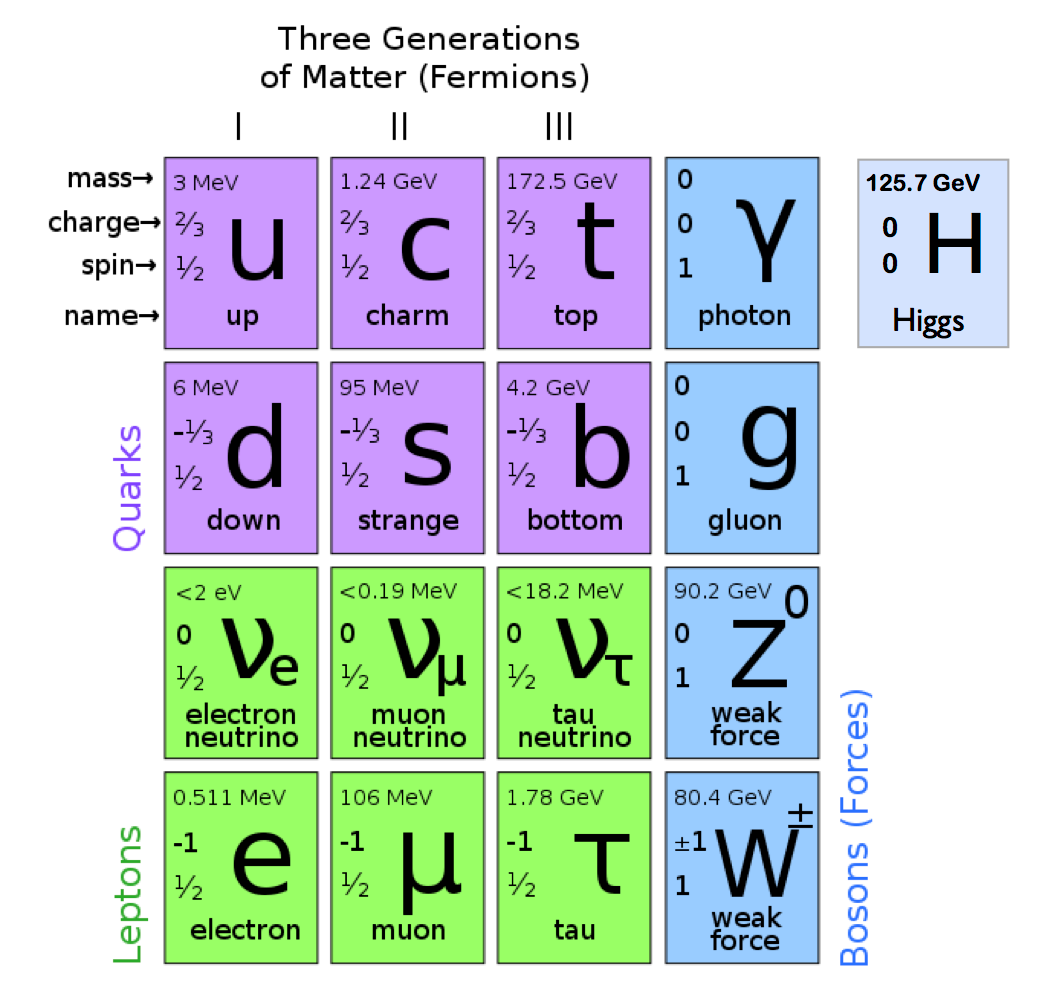
\includegraphics[width=0.55\textwidth]{graphics/Plots_Standard_Model.png}
    \caption{\sl The fundamental components of the \sm\ of particle physics.}
    \label{fig:ComponentsSM}
  }
\end{figure}
%The heaviest elementary particle in the \sm\ is the top quark.

The bosonic sector of the \sm\ consist of photon $\gamma$, $Z^0$ and $W^\pm$ bosons, gluons $g$, and scalar Higgs boson $H$.
 


\subsection{Fundamental Interactions}
\subsubsection{Electromagnetic interaction}
\label{sec:QED_SM}
%		QED
Quantum Electrodynamics (QED) is a quantum field theory, that describes an interaction between a fermionic field $\psi$ with a mass $m$ and a vector field $A_\mu$. 
The fermionic field has local $U(1)$ group invariance: %$$ group symmetry:
\begin{equation}
	\psi(x) \to e^{i\xi (x)}\psi(x).
\end{equation}
In order to preserve the local $U(1)$ symmetry, the vector field is required to be invariant under gauge transformation
\begin{equation}
A_\mu \to A_\mu (x) + \partial_\mu \xi(x).
\end{equation} 

The simplest QED Lagrangian density for a massless vector field is given by:
\begin{equation}
	\mathcal{L}_{QED}=i\bar{\psi}\gamma^\mu D_\mu \psi - \frac{1}{4}F_{\mu\nu}F^{\mu\nu},
    \label{formula:QEDlagrangian_1}
\end{equation}
where the strength tensor of the vector field is $F_{\mu\nu}=\partial_\mu A_\nu - \partial_\nu A_\mu$ and the covariant derivative is $D_\mu = \partial_\mu - ieQ A_\mu$, $e$ is a coupling constant and $Q$ is the electric charge of the fermion. 

Introduction of the covariant derivative enables fermion-photon interaction via the $-ieA_\mu\psi\gamma^\mu\bar{\psi}$ term and, moreover, it ensures the $U(1)$ symmetry in the Lagrangian density. According to the N\"other theorems, each symmetry of a Lagrangian correspond to a conserved current or charge, therefore, the $U(1)$ group symmetry of (\ref{formula:QEDlagrangian_1}) implies the conservation of the electric charge.

Scattering processes in quantum field theory can be calculated from the $S$-matrix, the time-evolution operator, which depends on the Lagrangian density of the theory. 

The fine structure constant characterizes a strength of electromagnetic interaction and it is defined in QED as $\alpha = \frac{e^2}{4\pi\epsilon_0}$. The measured value of the fine structure constant is approximately $1/137$, much smaller than 1, which allows to apply perturbation theory for $S$-matrix calculation. Each order of the perturbation series can be represented by a Feynman diagram, examples are given in Fig.~\ref{fig:FeynmanSM}. The resummation of the calculated perturbation terms is called renormalization, and it leads to the dependence of coupling constant on momentum transfer and to the corrections of particle masses. For QED the fine structure constant increases with energy and for $Z^0$ pole it has value of $\alpha(m_{Z_0}^2) \approx 1/128$.

\begin{figure}[h]
{\centering
    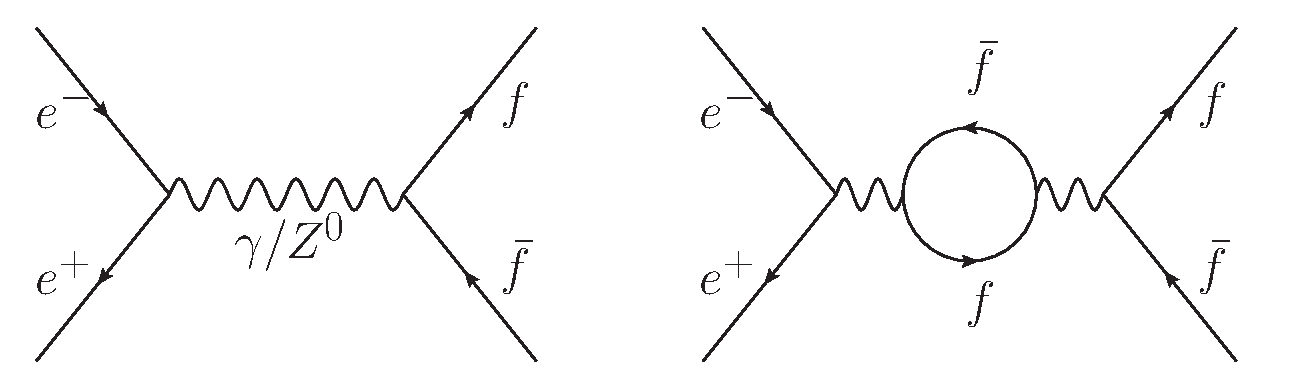
\includegraphics[width=0.55\textwidth]{graphics/FeynmanSM.eps}
    \caption{\sl Example of Feynman diagrams for $e^+e^- \to f\bar{f}$ process for Leading Order (left) and Next to Leading Order (right). }
    \label{fig:FeynmanSM}
  }
\end{figure}

QED is an accurate theory of electromagnetic interactions, that has been tested to a high precision. 
Towards the higher energies, other phenomena set in, which leads to the introduction of new forces and particles. 

%%%%%%%%%%%%%%%%%%%%%%%%%%%%%%%%%%%%%%%%%%%%%
%%%%%%%%%%%%%%%%%%%%%%%%%%%%%%%%%%%%%%%%%%%%%
%%%%%%%%%%%%%%%%%%%%%%%%%%%%%%%%%%%%%%%%%%%%%
\subsubsection{Electroweak interactions}
\label{sec:EWT_SM}
The first theory of weak interactions was developed by Fermi to describe the $\beta$ decays of unstable nuclei. The Fermi theory based on an interaction of fermionic currents without any gauge boson mediators. The Fermi coupling constant $G_F$ has a dimension of GeV$^{-2}$. This gives a strong evidence that this theory is not fundamental. The discovered weak bosons $Z^0$ and $W^\pm$ have masses far above typical energy transfer in radioactive decays of a nucleus, therefore, the Fermi theory is a low energy limit of modern Electroweak theory.

The experiments with $\beta$-decays of unstable nuclei in 1950's established maximal parity violation of weak charged currents, that involve only left-handed electrons and right-handed positrons. 

The unified theory of electroweak interaction, which was introduced by Glashow, Weinberg and Salam in 1960's, predicted the existence of weak neutral currents and the corresponding $Z^0$ boson, which can couple to right-handed particles. 
The first indications of weak neutral currents were observed at Gargamelle bubble chamber at CERN, and then, the discovery was confirmed by SPS experiments also at CERN in 1983. 

The weak interaction of the \sm\ is based on non-abelian $SU(2)_L$ symmetry group. The number of generators of a group is equal to number of gauge bosons in theory. However, taking into account the boundary condition of group unitarity, there are 3 bosons of weak force. 

The Electroweak theory operates massless $SU(2)_L$ gauge fields $W^a_\mu$ and $U(1)$ vector field $B_\mu$. The vector fields $W^a_\mu$ are initially coupled only to the left-handed fermion doublets.

The strength of the $SU(2)_L$ gauge field $W_m^a$ is defined as
\begin{equation}
	F_{mn}^a =  \partial_m W_n^a - \partial_n W_m^a + g \epsilon_{abc}W_m^b W_n^c,
    \label{formula:weakF_1}
\end{equation}
where $g$ is a coupling constant and structure constant $\epsilon_{abc}$ is the Levi-Civita tensor. The last term in (\ref{formula:weakF_1}) introduces gauge boson self-interactions, contrary to abelian QED model. 

One introduces weak mixing angle $\sin\theta_W$ relating the massless eigenstates of the weak fields and the physical mass eigenstates of the fields as:% along with the relation between massless weak eigenstate fields and physical mass eigenstate bosons:
\begin{equation}
\begin{array}{l}
W^\pm_\mu = \frac{1}{\sqrt{2}}(W^1_\mu \mp iW^2_\mu )\\
Z_\mu = W^3_\mu \cos\theta_W - B_\mu \sin\theta_W\\
A_\mu = W^3_\mu \sin\theta_W + B_\mu \cos\theta_W,
\end{array}
\label{formula:ZWafterSB_1}
\end{equation}
where $W^\pm_\mu$ and $Z_\mu$ are the physical states of the weak bosons, $A_\mu$ is the physical photon field. 
The electric coupling constant from QED is defined as 
\begin{equation}
e = g\sin\theta_w = g'\cos\theta_w,
\end{equation}
where $g$ and $g'$ are the coupling constants of weak eigenstate fields.

The Lagrangian density of mass eigenstates contains weak currents, that have a vector-axial vector (V-A) structure:
\begin{equation}
\mathcal{L}_{EW,int} = \frac{g}{2\sqrt{2}}\bar{\Psi}\gamma^\mu(1-\gamma^5)W^\pm_\mu\Psi' +\frac{g}{2\cos\theta_w} \bar{\Psi}\gamma^\mu(g_V-g_A\gamma^5)Z_\mu\Psi,
    \label{formula:weakLagrangian_1}
\end{equation}
where $g_V$ and $g_A$ are the vector and axial vector coupling constants of $Z^0$ boson to a fermionic field $\Psi$. 
As can be seen from (\ref{formula:weakLagrangian_1}), due to the mixing, the $Z^0$ boson is coupled to both, left-handed and right-handed, fermions, while the $W^\pm$ bosons are coupled only to the left-handed fermions.

The $Z^0$ and $W^\pm$ bosons acquire their masses via spontaneous symmetry breaking and the Higgs mechanism, described in Section \ref{sec:Higgs_SM}.

%%%%%%%%%%%%%%%%%%%%%%%%%%%%%%%%%%%%%%%%%%%%%
%%%%%%%%%%%%%%%%%%%%%%%%%%%%%%%%%%%%%%%%%%%%%
%%%%%%%%%%%%%%%%%%%%%%%%%%%%%%%%%%%%%%%%%%%%%

\subsubsection{Strong interaction}
\label{sec:QCD_SM}
The strong force is described by Quantum Chromodynamics (QCD), which is a relativistic quantum field theory based on $SU(3)$ symmetry.
The strong force is mediated by eight massless vector gauge bosons called gluons. 
General QCD Lagrangian density of quark fermion $q$ and gluon vector field $G^a_\mu$ is
\begin{equation}
	\mathcal{L}_{QCD}=\bar{q}(i\gamma^\mu D_\mu - M ) q - \frac{1}{4}G^a_{\mu\nu}G^{\mu\nu}_a,
    \label{formula:strongLagrangian_1}
\end{equation}
where the covariant derivative $D_\mu = \partial_\mu - i g t_a G^a_\mu$, $g_s$ is the strong coupling constant and $t_a$ are the Gell-Mann matrices being the generators of the $SU(3)$ group. The gluon field strength is
\begin{equation}
G^a_{\mu\nu}=\partial_\mu G^a_\nu - \partial_\nu G^a_\mu - g_s f_{abc}G_\mu^b G_\nu^c,
\end{equation}
where $f_{abc}$ is a structure constant tensor for $SU(3)$ group. 
Similarly to the weak interaction, QCD theory is based on a non-Abelian symmetry group and it also contains the vector boson self-interaction terms in the Lagrangian density. 

The non-Abelian quantum field with massless gauge bosons demonstrate different the asymptotic behavior of coupling constant: the strong fine-structure constant $\alpha_{s0} = g_s^2/(4\pi)$ depends on momentum transfer squared $Q^2$ as 
\begin{equation}
\alpha_{s}(Q^2) \propto ln^{-1}(Q^2),
\end{equation}
which means, that the strength of QCD interaction is decreasing for high energy processes. This effect of QCD is called asymptotic freedom. On the other hand, when momentum transfer is small, the $\alpha_{s}$ becomes large. Theoretical prediction of $\alpha_s(Q)$ and the results of $\alpha_s$ measurements are shown in Fig.~\ref{fig:alpha_s}. This behavior of $\alpha_s(Q)$ leads to the effect of color confinement, when quarks and gluons form colorless objects called hadrons. For low energy processes, the perturbation theory cannot be applied because of the strong QCD coupling. Therefore, the low-energy QCD processes and the color confinement effects are analyzed using Lattice QCD methods. 
\begin{figure}[h]
{\centering
    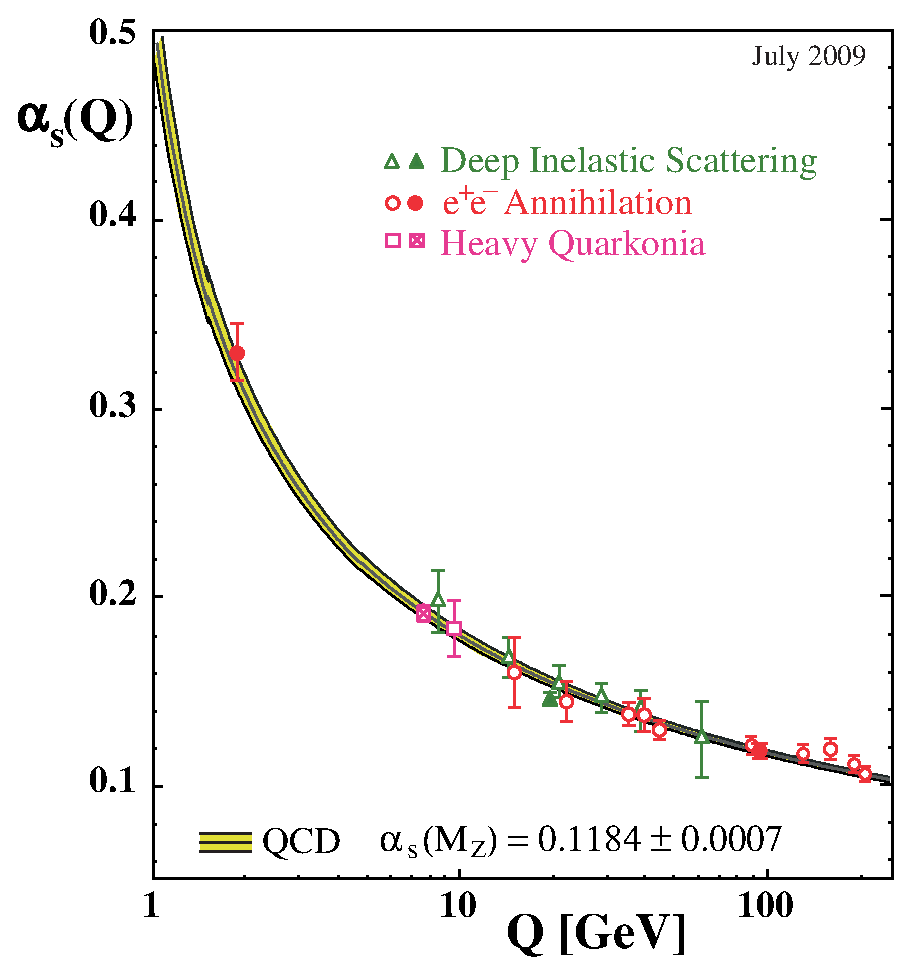
\includegraphics[width=0.45\textwidth]{graphics/asq-2009.eps}
    \caption{\sl Summary of measurements of $\alpha_s$ as a function of the energy scale $Q$.\cite{bib:alpha_s}}
    \label{fig:alpha_s}
  }
\end{figure}

%So far, the only quark, that does not have a hadronic final state is the top quark. Because of its high mass, it decays via weak interaction before a formation of any hadronic states. 

%%%%%%%%%%%%%%%%%%%%%%%%%%%%%%%%%%%%%%%%%%%%%
%%%%%%%%%%%%%%%%%%%%%%%%%%%%%%%%%%%%%%%%%%%%%
%%%%%%%%%%%%%%%%%%%%%%%%%%%%%%%%%%%%%%%%%%%%%

\subsection{The Higgs mechanism}
\label{sec:Higgs_SM}
% Higgs is the only elementary scalar in the \sm
%Why?
%Goldstone bosons???
Classical mass terms for quantum fields without symmetry breaking mechanism cause the following problems:
\begin{itemize}
	\item Term $m_A A_\mu A^\mu$ for a vector field $A_\mu$ introduce an ultraviolet divergence in the massive vector field propagator;
	\item Terms like $m_\psi\psi_L \psi_R$ are not gauge-invariant, since right-handed and left-handed fermions have different set of quantum numbers in the \sm.
\end{itemize}
The mechanism of spontaneous symmetry breaking or the Higgs mechanism is an essential part of fundamental physics. 
It allows to include the weak vector boson masses in a renormalizable way and to  preserve the gauge invariance of fermion mass terms in the Lagrangian density of the \sm. 

%DOUBLET
The spontaneous symmetry breaking mechanism starts from a complex scalar field doublet $\phi$ , which has initially four degrees of freedom. 
The Lagrangian density, related to the scalar field, which is coupled to $SU(2)$ gauge field $W_\mu$ and $U(1)$ vector field $B_\mu$, has the following terms: 
%The higgs symmetry???
\begin{equation}
	\mathcal{L}_{H} = \frac{1}{2}(D_\mu\phi)^2 - V(\phi),
    \label{formula:scalarLagrangian_1}
\end{equation}
where covariant derivative $D_\mu = \partial_\mu - i g \tau_a W^a_\mu - ig'/2 B_\mu$ and the matrices $\tau_a$ are the $SU(2)$ group generators. This Lagrangian density has a $SU(2) U(1)$ symmetry.
The form of the scalar field potential $V(\phi)$ is in general case 
\begin{equation}
    V(\phi) = -\frac{1}{2}\mu^2|\phi|^2 +  \frac{1}{4} \lambda |\phi|^4.
\end{equation}
If the parameter $\mu^2 > 0$, the scalar field $\phi$ will acquire a nonzero vacuum expectation value  %and the $SU(2)$ local symmetry will be broken:
\begin{equation}
\phi_0 = \frac{1}{\sqrt{2}}
\begin{pmatrix}
0\\v
\end{pmatrix} \text{ and } v = \sqrt{\frac{\mu^2}{\lambda}}, 
\end{equation}
which breaks local $SU(2)$ symmetry of the Lagrangian density. 

According to the Goldstone theorem, number of broken group generators correspond to the number of massless scalar particles called Goldstone bosons. 
In the \sm\ case, the broken $SU(2)$ symmetry produces three Goldstone bosons and one Higgs boson $H$, which has a leftover degree of freedom from the initial scalar doublet $\phi$.
The three Goldstone bosons are absorbed as longitudinal degrees of freedom by vector fields $W^a_\mu$, thus giving mass to the weak bosons.

The relevant terms after symmetry breaking from (\ref{formula:scalarLagrangian_1}) are
\begin{equation}
	\Delta \mathcal{L}_{H} = \frac{1}{2} \frac{v^2}{4}[g^2 (W^1_\mu)^2 + g^2 (W^2_\mu)^2 + (-g W^3_\mu + g' B_\mu)^2].
\end{equation}
The electroweak fields acquire physical states (\ref{formula:ZWafterSB_1}) with masses
\begin{equation}
\begin{array}{l}
m_W^\pm = g\frac{v}{2},\\
m_Z^0 = \sqrt{g^2 + g'^2}\frac{v}{2},\\
m_A = 0,
\end{array}
\label{formula:ZWmassafterSB_1}
\end{equation}
and the Higgs boson mass is
\begin{equation}
m_H = \sqrt{2\lambda}v.
\end{equation}

With postulated quantum numbers of the Higgs field, one writes the gauge-invariant mass terms for a fermion $\psi$ as 
\begin{equation}
	\Delta \mathcal{L}_\psi = -\lambda_\psi \Psi_L \phi \psi_R,
\end{equation}
where dimensionless parameter $\lambda_\psi$ is a Higgs coupling to the fermion field, $\Psi_L$ is the left-handed $SU(2)$ doublet, and $\psi_R$ is the right-handed $SU(2)$ singlet. Thus, this expression has zero sum of the hypercharge $Y$, and it can be extended to all lepton particles of the \sm. The mass terms for the quark sector are more complicated, because of involvement of quark mixing, but the expression for fermion mass is universal
\begin{equation}
	m_\psi = \frac{1}{\sqrt{2}} \lambda_\psi v.
    \label{formula:fermionMass_1}
\end{equation}
% Higgs - top relation

The discovery of the Higgs scalar by LHC collaborations (see Fig.~\ref{fig:diphoton}) added the last missing piece to the \sm, and experimentally proved the principles of the mechanism of spontaneous symmetry breaking.

The expressions \ref{formula:ZWmassafterSB_1} and \ref{formula:fermionMass_1} suggest a simple linear relation between Higgs boson couplings and masses of corresponding particles. The results of the LHC experiments confirm this prediction within experimental uncertainties, as shown in Fig~\ref{fig:higgs_masses}.


\begin{figure}
\centering
\begin{subfigure}{0.5\textwidth}
\centering
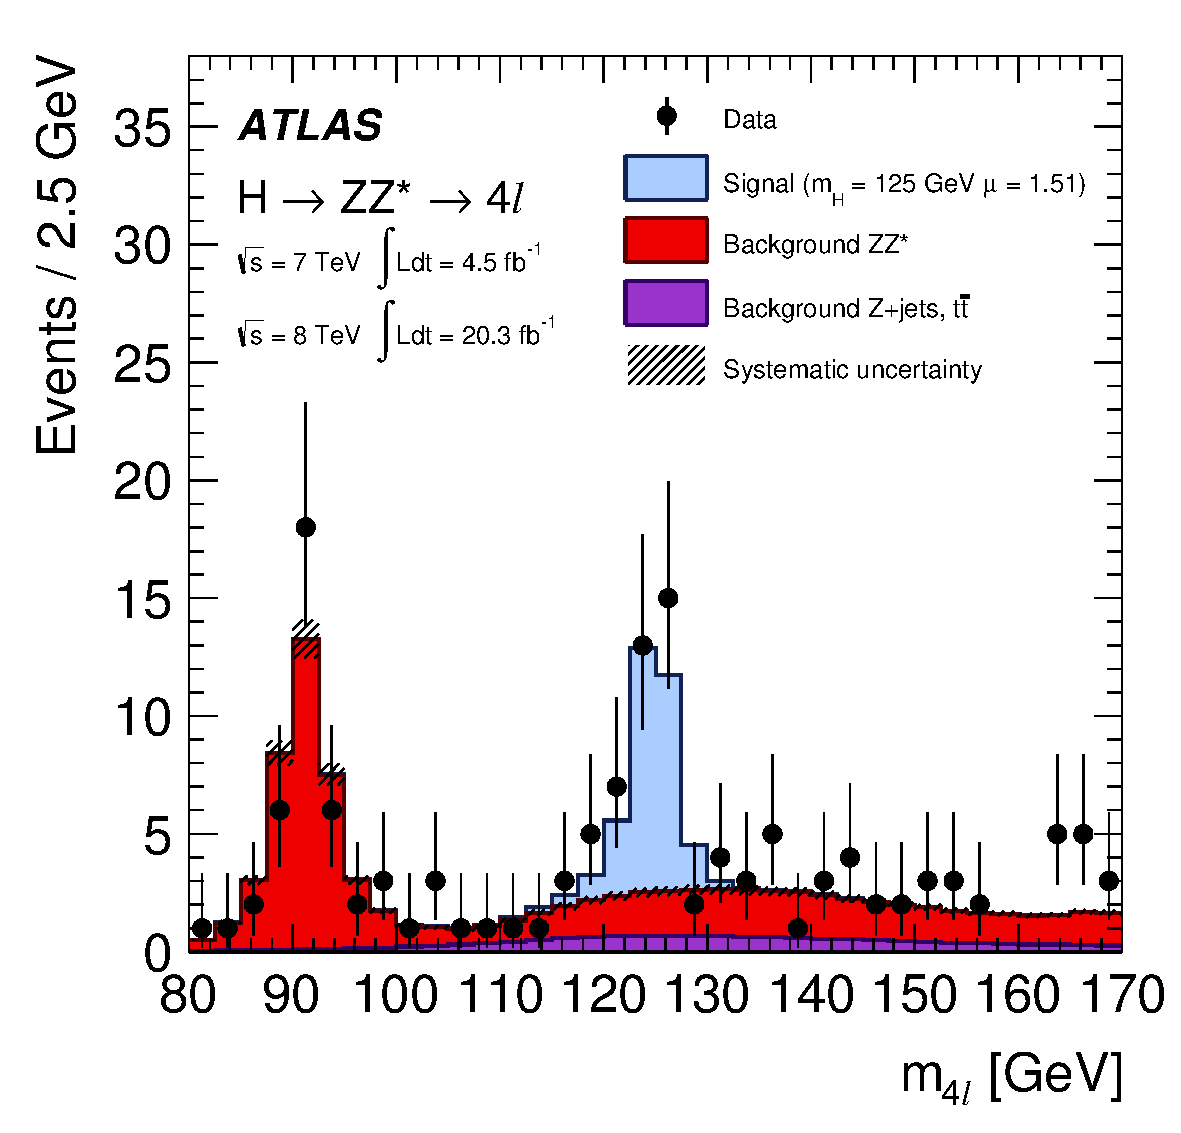
\includegraphics[width=.90\linewidth]{graphics/m4l_80_170_allYear_125.pdf}

\end{subfigure}% 
\begin{subfigure}{0.5\textwidth}
\centering
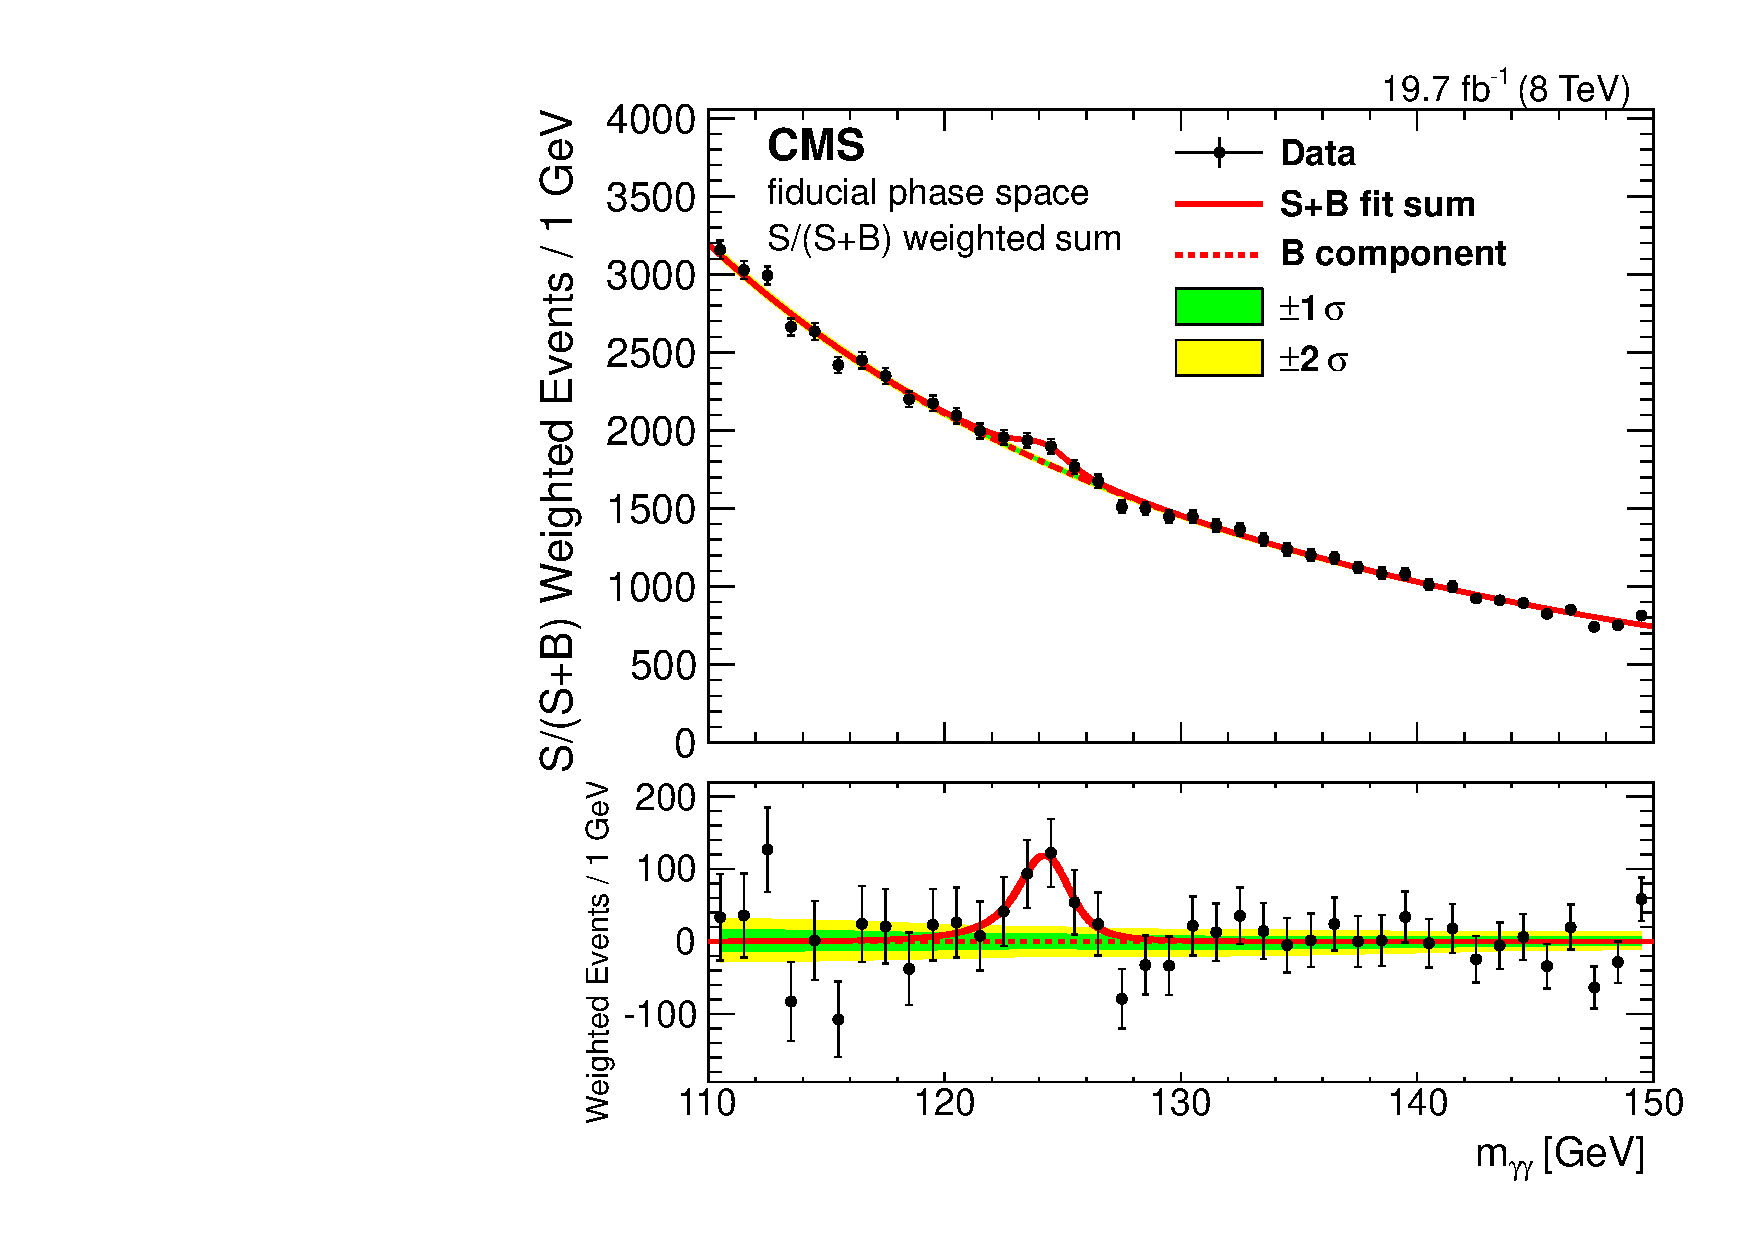
\includegraphics[width=.90\linewidth]{graphics/CMS-HIG-14-016_Figure_003.pdf}

\end{subfigure}
    \caption{\sl The Higgs boson signal in $Z^0Z^0$ channel by ATLAS (left) \cite{bib:HiggsAtlas2} and Higgs boson signal in diphoton invariant mass distribution by CMS experiment (right) \cite{bib:HiggsCms2}.}
    \label{fig:diphoton}
\end{figure}

\begin{figure}
{\centering
    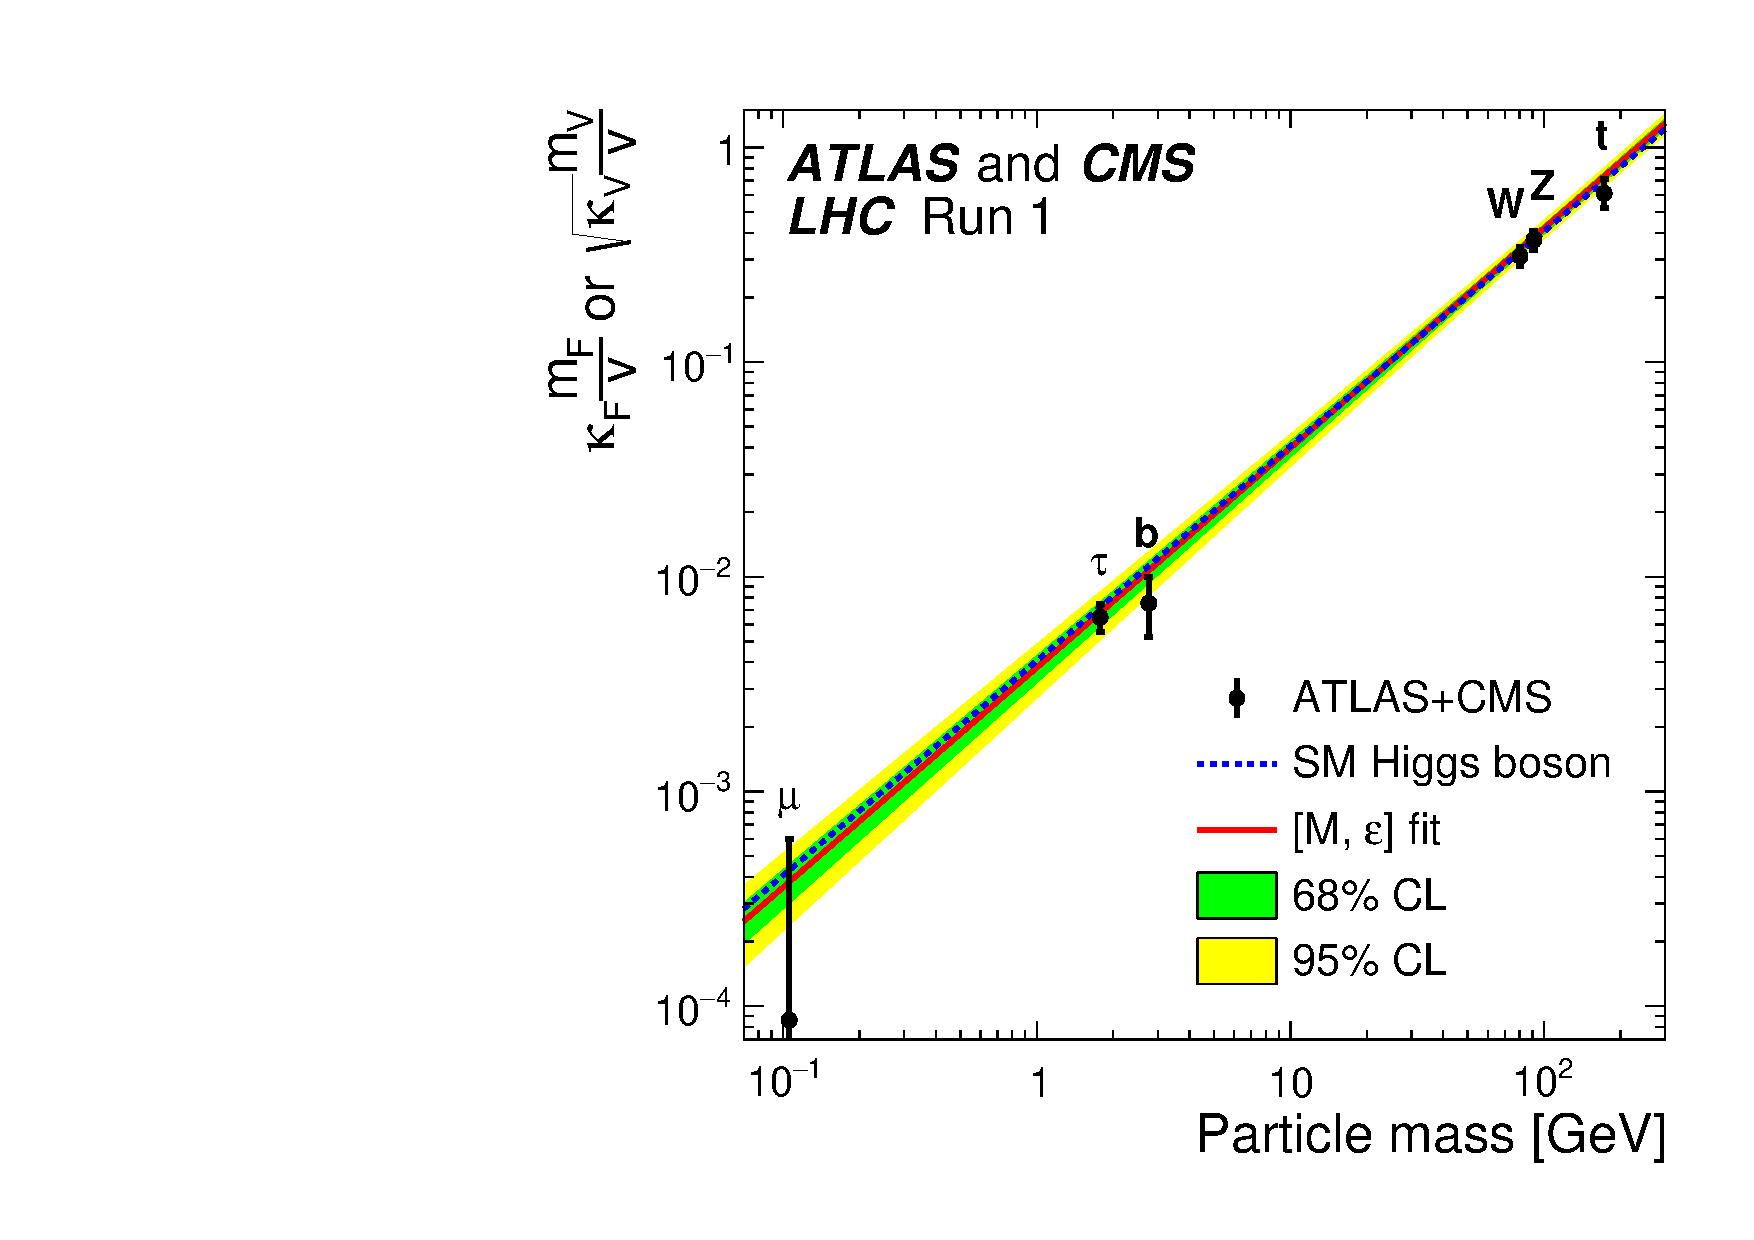
\includegraphics[width=0.45\textwidth]{graphics/Meps_lhc.pdf}
    \caption{\sl Demonstration of the linear dependence of particle masses on Higgs boson couplings by LHC experiments. \cite{bib:HiggsLhc2}}
    \label{fig:higgs_masses}
  }
\end{figure}

\subsection{The \sm\ tests and open questions in particle physics}
\label{sec:Problems_SM}
The \sm\ results from the synergy between theoretical ideas and experimental results. After finalization of the \sm\ framework, this model was able to predict many crucial phenomena of particle physics, like the existence of weak neutral currents, top quark and Higgs boson.
The \sm\ has been tested to a high precision at the machines like HERA, SLC, LEP, TeVatron and LHC. A summary of electroweak precision measurements compared to a \sm\ electroweak fit values is shown in Fig.~\ref{fig:SM3deviations}. The \sm\ fit demonstrates, that there are no deviation greater than 2.5~$\sigma$. 

\begin{figure}[ht]
\centering
  \includegraphics[width=0.46\textwidth]%
                  {graphics/2014_07_16_PullPlotTwoBarsTwoTheos_logo.eps}
  \caption{Deviations of the electroweak precision
observables in the Standard Model~\cite{bib:AfbSMFit}. }
  \label{fig:SM3deviations}
\end{figure}
%The muon g-2 experiments can measure muon  
The \sm\ prediction of the $\mathcal{CP}$ violation has been confirmed by the B-meson experiments. 
%The experiments, that explore rare $B$-meson decays, like BaBar, Belle or LHCb, show a good agreement with the \sm\ predictions. 
Nevertheless, some experiments in particle physics as well as a few cosmological observations have tensions with the \sm\ predictions.
The shortcomings of the \sm\ can be summarized as following:
\begin{itemize}
%Gravity
\item The \sm\ provide precise and consistent explanation of interactions between three out of four fundamental forces, the gravitational force is not included. The integration of the gravity into the \sm\ framework is unsuccessful, because of non-renormalizablity of tensor quantum fields. Knowledge of quantum gravity is important for cosmology of early Universe and for physics of extremely massive astrophysical objects, like black holes.
%Higgs mass fine-tuning
\item Quantum corrections to the Higgs boson mass are large comparing to the mass of Higgs boson itself, which resembles a \textit{fine-tuning problem} of the \sm. This can be avoided if there are new massive bosons, that can stabilize the Higgs mass corrections.
\item There is no explanation of the reason behind the spontaneous symmetry breaking mechanism in the \sm\ framework. 

% mass hierarchy 
\item The particle masses in the \sm\ are proportional to the Higgs coupling constants, which are input parameters of the theory. Thus, the \sm\ do not provide any explanation of 6 orders of magnitude difference between well measured electron mass and top quark mass. This fact is known as a \textit{mass hierarchy problem}.

\item The sources of the charge-parity ($CP$) asymmetry, provided by the quark mixing matrix in the \sm, are too small to explain the \textit{matter-antimatter asymmetry} of the Universe.
\item Anomalous rotation of galaxies suggests an existence of large amount of \textit{dark matter} - massive particles, that do not interact with electromagnetic field. The \sm\ neutrinos are too light to explain this observation, therefore, the \sm\ has no candidate particle for dark matter. 
%Afb bbbar
%g-2

\end{itemize}



Many \bsm\ theories propose elegant solutions to the shortcomings of the \sm\ mentioned above, and many experiments are looking for their evidences. 
This thesis proposes new tests of the \sm\ using the ILC project, which will provide new evidences of New Physics with a discrimination power between different \bsm\ theories.
%At the same time, there is a lack of knowledge about many input parameters of the \sm, and high precision measurements can give further hints for New Physics.

%Dark matter there are many theoretical solutions that resemble gravity modifications


\newpage
%%%%%%%%%%%%%%%%%%%%%%%%%%%%%%%%%%%%%%%%%%%%%
%%%%%%%%%%%%%%%%%%%%%%%%%%%%%%%%%%%%%%%%%%%%%
%%%%%%%%%%%%%%%%%%%%%%%%%%%%%%%%%%%%%%%%%%%%%

\section{The International Linear Collider}
\label{sec:ILC}
\subsection{Role in particle physics}
Particle accelerators, that produce colliding beams, colliders, drive the progress of our understanding of the subatomic world.

For particle physics, mainly two types of colliders are relevant:
\begin{itemize}
\item Hadron colliders have beams of proton and/or antiproton, for example SppS, TeVatron or LHC;
\item Lepton colliders collide electron and positron beams, for example SLC, PETRA or LEP.
\end{itemize}

%The hadron colliders are generally considered as a "discovery" machines due to their higher center-of-mass energy, while electron-positron colliders mostly used for a consolidation of theoretical conclusions by high-precision measurement of theory parameters. 
%LHC is great 

The Large Hadron Collider is the most powerful proton-proton collider ever made and it has already made a breakthrough by discovering the Higgs boson.  Nevertheless, to measure precisely all accessible properties of the Higgs particle and other \sm\ particles scientific community needs a new high-precision experiment.

It is a worldwide consensus, that the next large high-energy physics facility after LHC should be a lepton collider. 
The main advantages of a lepton collider over the hadron machines are a well-known initial state of colliding particles and a higher signal to background ratio for many physics processes.
The linear electron-positron colliders, like SLC at Stanford, have higher energy reach, more focused beams having more compact accelerator complex, than the equivalent circular machines.

The International Linear Collider is a project of linear electron-positron collider designed for energies between 250\,GeV and 1000\,GeV. 
The Compact Linear Collider (CLIC) is an alternative project of a future electron-positron machine with a nominal $\sqrt s$ of 3\,TeV. 
This thesis is focused on the ILC project.
%The ILC Technical Design Report (TDR)~\cite{bib:ILC} is the result of many years of of globally coordinated research and development. 
%Its parameters have been set by physics requirements and reviewed continuously by a wide scientific community. The R\&D was summarized in the Technical Design Report (TDR).~\cite{bib:ILC}
The ILC is designed for searches of New Physics and high-precision measurements of the \sm\  parameters. 
The ILC physics program is oriented on the production thresholds of heavy \sm\ particles the Higgs and the top quark. 
The physics potential of the ILC project will be enhanced by polarized beams, which can be used to suppress background processes in electroweak physics. 


%According to these features, the ILC has a rich physics program, precision measurements of the \sm\ parameters, as well as direct and indirect searches of New Physics. 
%%%%%%%%%%%%%%%%%%%%%%%%%%%%%%%%%%%%%%%%%%%%%
%%%%%%%%%%%%%%%%%%%%%%%%%%%%%%%%%%%%%%%%%%%%%
%%%%%%%%%%%%%%%%%%%%%%%%%%%%%%%%%%%%%%%%%%%%%


\subsection{Research program at the International Linear Collider}

Following the discovery of the Higgs boson by the LHC experiments, the ILC will complement the LHC discovery by measuring precisely all accessible properties of this particle.
The main advantage of the ILC is a model-independent measurement of electroweak parameters.
The model-independent measurement of the Higgs properties is done by studying the Higgs-strahlung $e^+e^-\to Z^0H$ process.
The ILC experiments will measure the full width of Higgs decay, which is impossible at the LHC environment. 

%No information on the BSM
%ILC is an ideal machine to look for invisible Higgs decays or light dark matter searches, due to its high detector hermeticity. 

%The nominal center-of-mass energy of the ILC is 500\,GeV, which can be increased up to 1\,TeV. 
The ILC can run at the center-of-mass energy of 250\,GeV, which gives the peak production for the  Higgs-strahlung reaction. 
The top mass can be precisely measured at 350\,GeV energy, at the top pair production threshold. 
The couplings of the Higgs and top particles can be studied at 500\,GeV, as well as at 1\,TeV center-of-mass energy.
Therefore, the physics program covers several important thresholds in the \sm\ physics, that are summarized in Table~\ref{table:SMILCmeasurements}. 


\begin{table}[H]
\centering

\begin{tabular}{@{}rll@{}}
\toprule
Energy & Process & Goal of measurements\\ 
\midrule

91\,GeV  & $e^+e^- \to Z^0$  		& $Z^0$ physics and calibration \\
250\,GeV & $e^+e^- \to Z^0H$  		& Higgs couplings \\
		 & $e^+e^- \to f\bar{f}$  	& $Z^0/\gamma$ couplings \\
350\,GeV & $e^+e^- \to t\bar{t}$ 	& top mass precision \\
		 & $e^+e^- \to \nu\bar{\nu}H$ & Higgs couplings \\
500\,GeV & $e^+e^- \to t\bar{t}$ 	& top couplings \\
 		 & $e^+e^- \to t\bar{t}H$ 	& Higgs-top coupling \\ 
 		 & $e^+e^- \to Z^0HH$ 		& Higgs self coupling \\ 
1000\,GeV & $e^+e^- \to \nu\bar{\nu}HH$&  Higgs self coupling \\
 \bottomrule
\end{tabular}

\caption{\sl Major \sm\ processes to be studied at ILC. \cite{bib:ILC}}
\label{table:SMILCmeasurements}
\end{table}

%SM is a chiral theory 

%The variable center-of-mass energy of the collisions will provide an information on energy dependence of many important \sm\ parameters. 
 
%The ILC will resolve the ambiguities of the \sm\ electroweak fit, displayed in Fig.~\ref{fig:SM3deviations}, in a clear and definite way. 

%top
%Along with the Higgs boson, the top quark has never been studied in electroweak environment of electron-positron colliders. 
%The access to the electroweak coupling constant of the top quark is limited for hadron colliders, while the ILC can measure these values to a percent precision.

Besides the \sm\ precision measurements, the ILC has a rich program of New Physics searches. 
There are huge variety of studies made by ILC community, dedicated to the direct searches of the dark matter, additional particles from supersymmetric theories, indirect searches of resonances from extradimentional models, etc.
Entire physics program is improved  by beam polarization, which will deliver a more detailed information on the \sm\ coupling constants, and more control over background process rates. 
%The production of the top quark for the hadronic machines, like TeVatron or LHC, is via the gluon splitting, while at the ILC, the dominant top quark production is
% 3 important thresholds ZH, tt, ZHH
% beam polarisation 
\subsubsection{Operating scenarios of the ILC}
\label{sec:ILCOperation}
The ILC running scenarios are described in Ref.~\cite{bib:H20}. 
The preferable running option is called H-20, which is optimized to reach the desired accuracies on the \sm\ couplings during 20 years of ILC operation. 
The accumulation of the integrated luminosity with time in this scenario is shown in Fig.~\ref{fig:H20}.
The foreseen luminosity upgrade of the accelerator complex~\cite{bib:LumiUp} allows to  increase significantly the collision event rate. 

\begin{figure}
	{\centering
		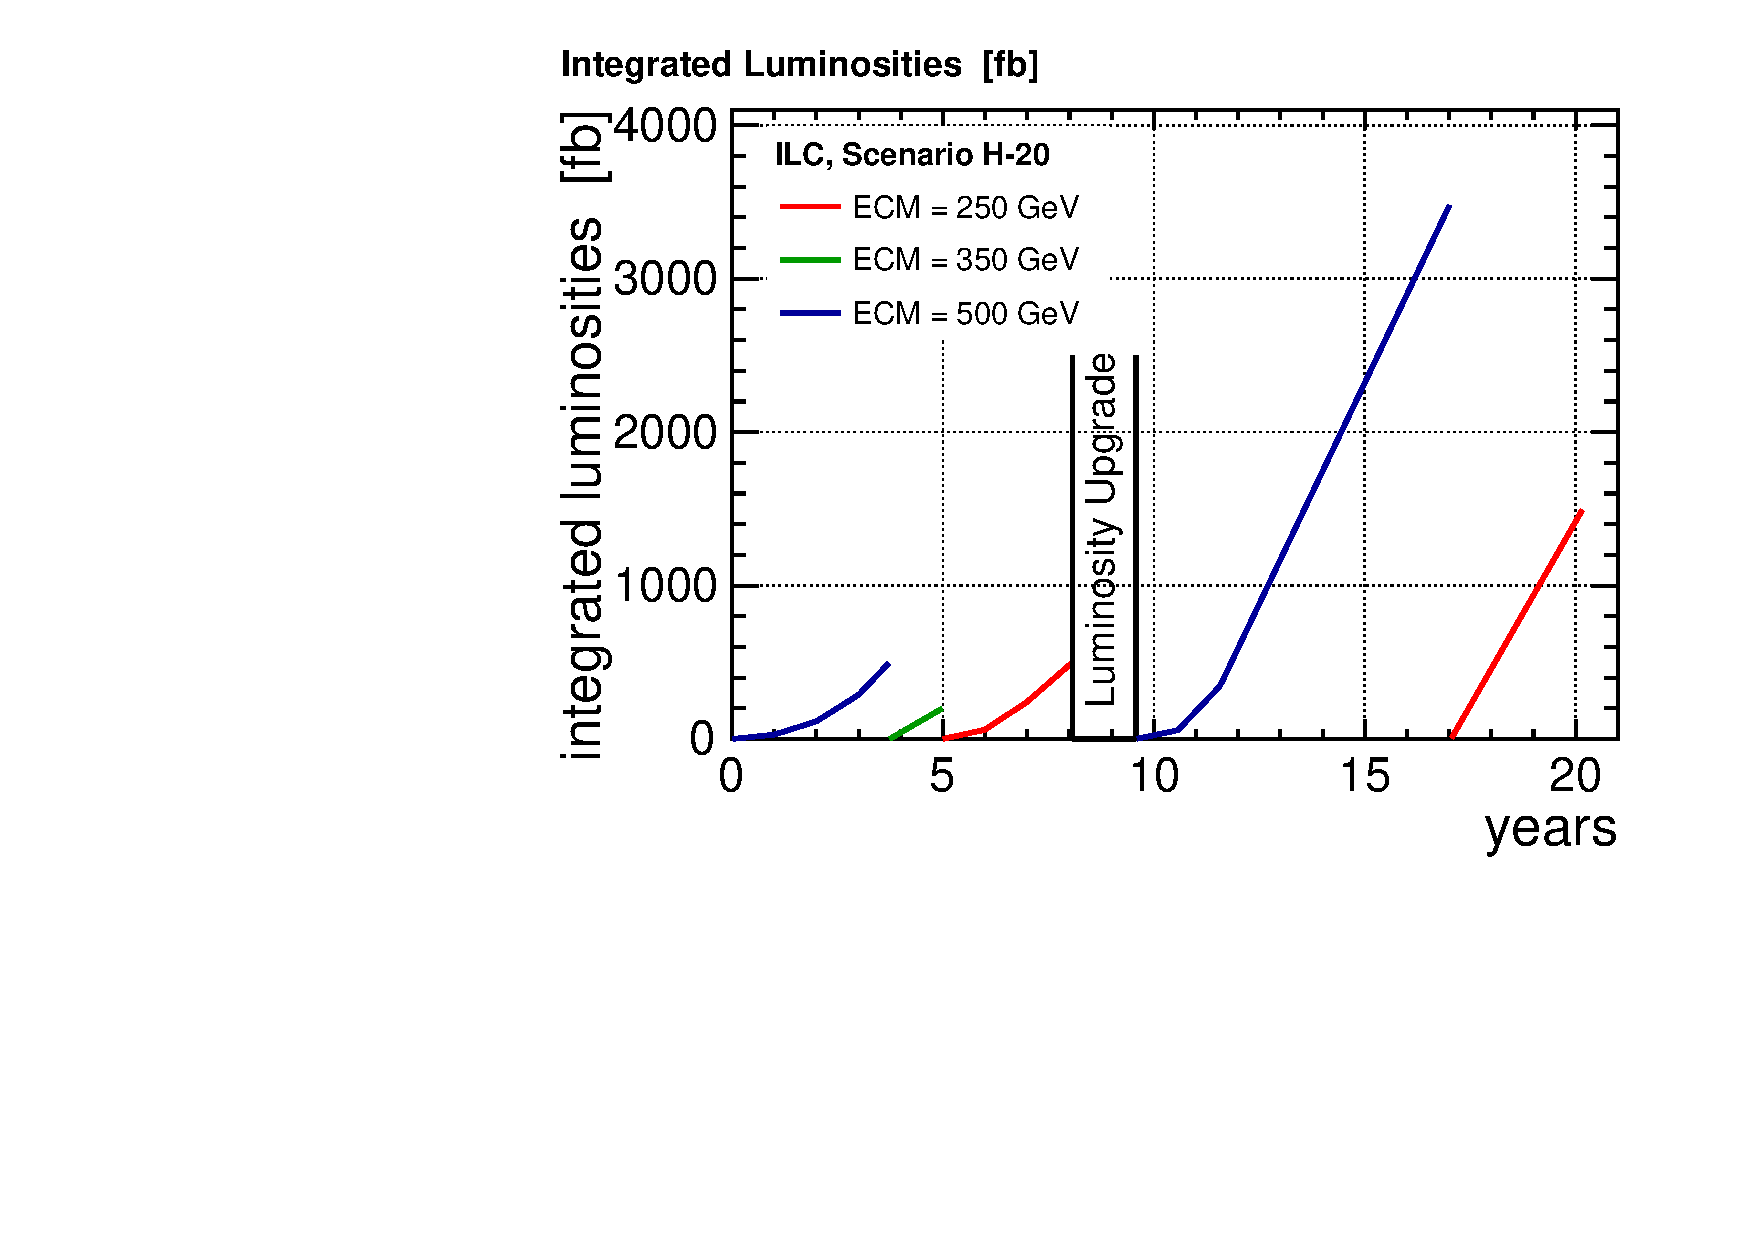
\includegraphics[width=0.55\textwidth]{graphics/lumi_H-20.pdf}
		\caption{\sl Accumulation of integrated luminosity versus real time in calendar years for scenario H-20.}
		\label{fig:H20}
	}
\end{figure}
In the H-20 scenario, the ILC physics program starts directly at 500\,GeV center-of-mass energy by collecting 500\ifb\ integrated luminosity. This choice makes possible to study all \sm\ processes from the beginning of the ILC physics operation.
The ILC will next collect 500\ifb\ integrated luminosity at $\sqrt{s} = 250$\,GeV before the luminosity upgrade.
The luminosity sharing between the different beam polarizations is described in Table~\ref{tab:H20}. 

\begin{table}[h]
\centering
  \renewcommand{\arraystretch}{1.10}
\begin{tabularx}{\textwidth}{*{5}{>{\centering\arraybackslash}X}}    %\begin{tabular*}{\textwidth}{@{\extracolsep{\fill}}|c|c|c|c|c|}
%\begin{tabular}{|l|c|c|c|c|}
\hline
        &  \multicolumn{4}{c}{integrated luminosity with $\operatorname{sgn}(P(e^-),P(e^+))= $ } \\
           & (-,+)       & (+,-)       & (-,-)       &  (+,+)     \\
\hline
$\sqrt{s}$ & [fb$^{-1}$] & [fb$^{-1}$] &  [fb$^{-1}$] & [fb$^{-1}$] \\ 
\hline
250\,GeV    &  1350      &  450        &  100	      &   100  \\
350\,GeV    &   135      &   45	       &   10	      &    10  \\
500\,GeV    &  1600      & 1600        &  400	      &   400  \\
\hline
\end{tabularx}
\caption{Integrated luminosities per beam helicity configuration in scenario H-20~\cite{bib:H20}.
}
\label{tab:H20} 
\end{table}

The beam helicity configuration of $e^-_Le^+_R$ or $(-,+)$ is called the left-handed beam configuration throughout the thesis, and the $e^-_Re^+_L$ or $(+,-)$ configuration is called the right-handed beam configuration. 

Currently, the ILC community considers the start of the physics program at $\sqrt{s} = 250$\,GeV and  the $\sqrt{s} = 500$\,GeV operation as an energy upgrade.

%%%%%%%%%%%%%%%%%%%%%%%%%%%%%%%%%%%%%%%%%%%%%
%%%%%%%%%%%%%%%%%%%%%%%%%%%%%%%%%%%%%%%%%%%%%
%%%%%%%%%%%%%%%%%%%%%%%%%%%%%%%%%%%%%%%%%%%%%

\subsection{Accelerator complex}
\label{sec:ILCacc}
Electrons and positrons are the lightest charged particles, therefore they have preference to emit a synchrotron radiation in a magnetic field. For circular accelerators the synchrotron radiation $E_{rad}$ strongly depends on the radius of accelerator $r$, particle mass $m$ and particle energy $E$ as
\begin{equation}
	E_{rad} \propto \frac{E^4}{m^4r}.
\end{equation}
This is the main limitation of circular electron-positron colliders, where dipole magnets of their accelerator system cause strong beam energy losses. 
The linear accelerator design avoid these drawbacks.

%CHANGE !!!!!!!!!!!
However, the linear accelerator design implies many challenges: high acceleration gradients are required to achieve the full beam energy in a single pass and the beams must have a high intensity and be focused into small spotsizes to achieve high collision rates, since the beams intersect only once.
% synchrotron radiation
% Years of R&D 

The schematic view of the entire accelerator system in  Fig.~\ref{fig:ILCScheme}. 
\begin{figure}
{\centering
    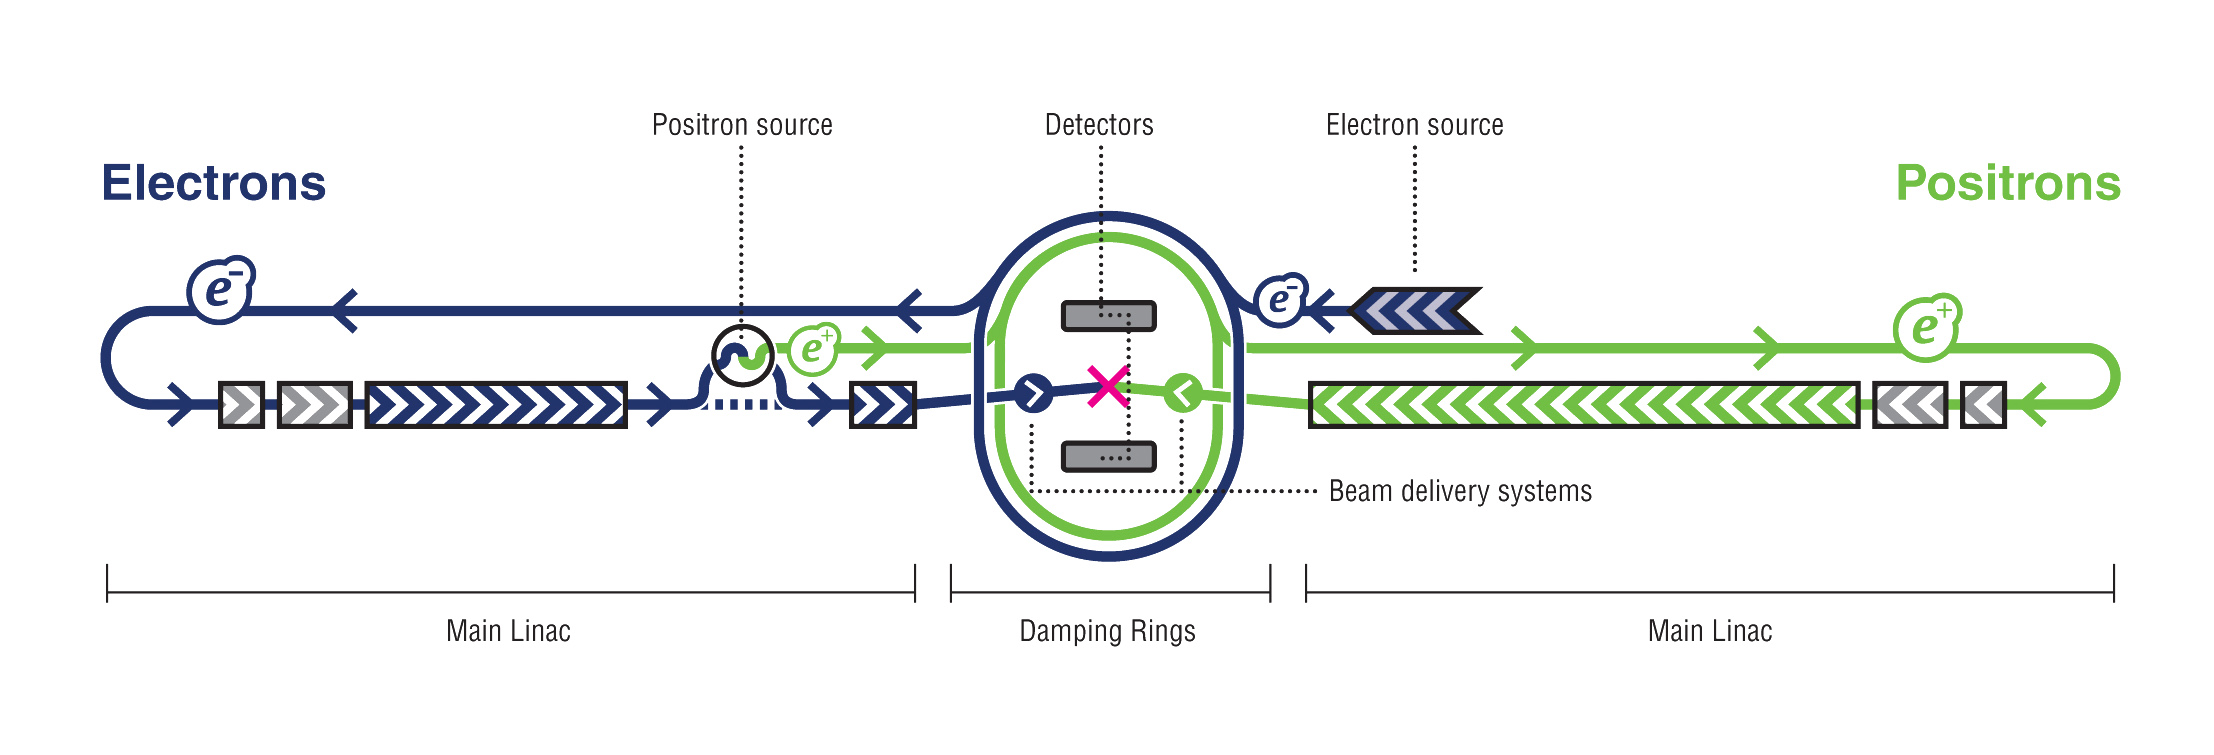
\includegraphics[width=0.95\textwidth]{graphics/ILC_scheme.jpg}
    \caption{\sl Schematic view of the ILC accelerator complex.}
    \label{fig:ILCScheme}
  }
\end{figure}
%The ILC accelerator complex is the result of more than a decade of a detailed research and development. 
The major sub-systems of the ILC accelerator are:
\begin{itemize}
\item a photocathode DC gun as polarized electron source
\item an undulator on the main electron beam accelerator as a polarized positron source
\item 5\,GeV electron and positron dumping rings to reduce a phase space of the initial particles
\item positron and electron 11\,km linear accelerators or linacs, composed of 1.3\,GHz cavities
\item a beam delivery system to bring the beams to the interaction point, which is shared by two detectors with push-pull configuration.
\end{itemize}
The main parameters of the beams, produced by the linac complex are given in Table~\ref{tab:ILCparam}.

\textit{The polarized electron beam} is obtained by sending a laser beam on a strained superlattice GaAs cathode which emits a bunch of electrons with high polarization. Then, the electrons are accelerated to 5\,GeV and injected into the electron damping ring.

\textit{The polarized positrons} are obtained by selecting positrons from $e^+ e^-$ pairs, created by converting polarized high energy photons on a rotating Ti-alloy target. The polarized photons are radiated by passing electrons in a superconducting helical undulator on the main electron beam.
A detailed layout of positron source is shown in Fig.~\ref{fig:ILCeplus}.
Similar to the electrons, the positron beam is accelerated to 5\,GeV energy in a superconducting linac before injection into the positron dumping ring. 

\begin{figure}
{\centering
    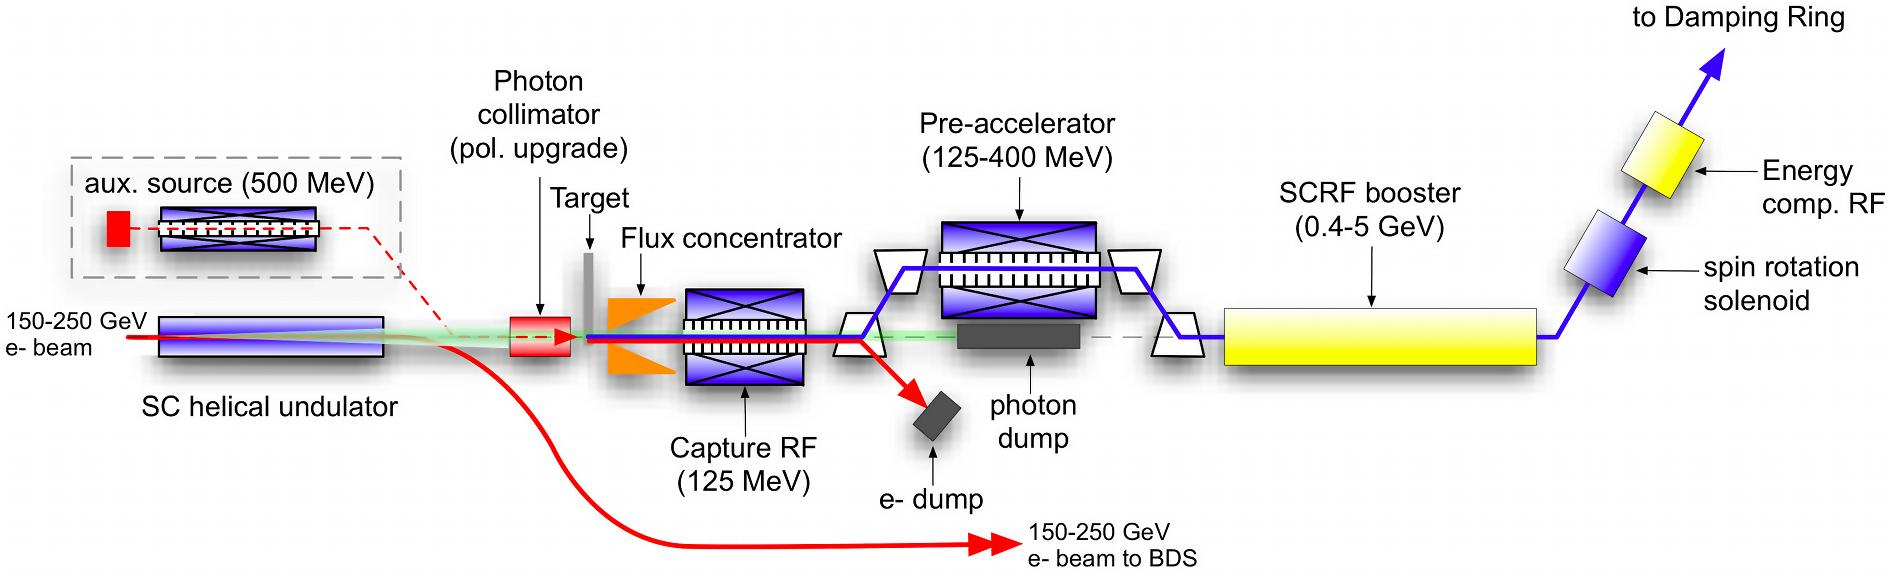
\includegraphics[width=0.95\textwidth]{graphics/ILCeplus.jpg}
    \caption{\sl Schematic view of the ILC positron source.}
    \label{fig:ILCeplus}
  }
\end{figure}

\textit{The damping rings} are housed in a common tunnel with circumference of 3.2\,km. They accept electrons and positrons with large transverse and longitudinal emittances and damp them to the low emittances needed for injection into the main linac. 
Each damping ring accommodates the injection and extraction systems, RF cavities and dumping wigglers.
The damping is made by an array of superferric wigglers in both dumping rings, which operate at 4.2\,K with 2.16\,T magnetic field. 
Both damping rings are connected to the main linear accelerators by transfer lines.

\textit{The main linear accelerators} are designed to accelerate the particles from 15\,GeV to a nominal energy of 250\,GeV. 
The acceleration is provided by approximately 7400 superconducting radio-frequency nine-cell niobium cavities (see Fig.~\ref{fig:ILCcavity}) operating at 2\,K temperature. 
The baseline accelerating gradient of the cavities is 31.5\,MV/m. 
The industrial mass production of the cavities can cause a random gradient variation of $\pm$20\%. 
The linac is able to produce bunches with a 554\,$\mu$m interval with 1312 bunches per beam pulse.
The balance between key parameters is a result of years of intensive R\&D by a wide scientific community. 
The cavities are assembled into two types of cryomodules: type A with nine SCRF cavities and type B with eight SCRF cavities and one superconducting quadrupole magnet located at the center of the module. 
The technology of industrial production of the cavities for ILC is a great challenge and there is room for improvement in accelerating gradient and efficiency. 
Same technology of SCRF cavities with lower average accelerating gradient is already implemented for electron acceleration at XFEL project in DESY~\cite{Abela:77248}. 
\begin{figure}
{\centering
    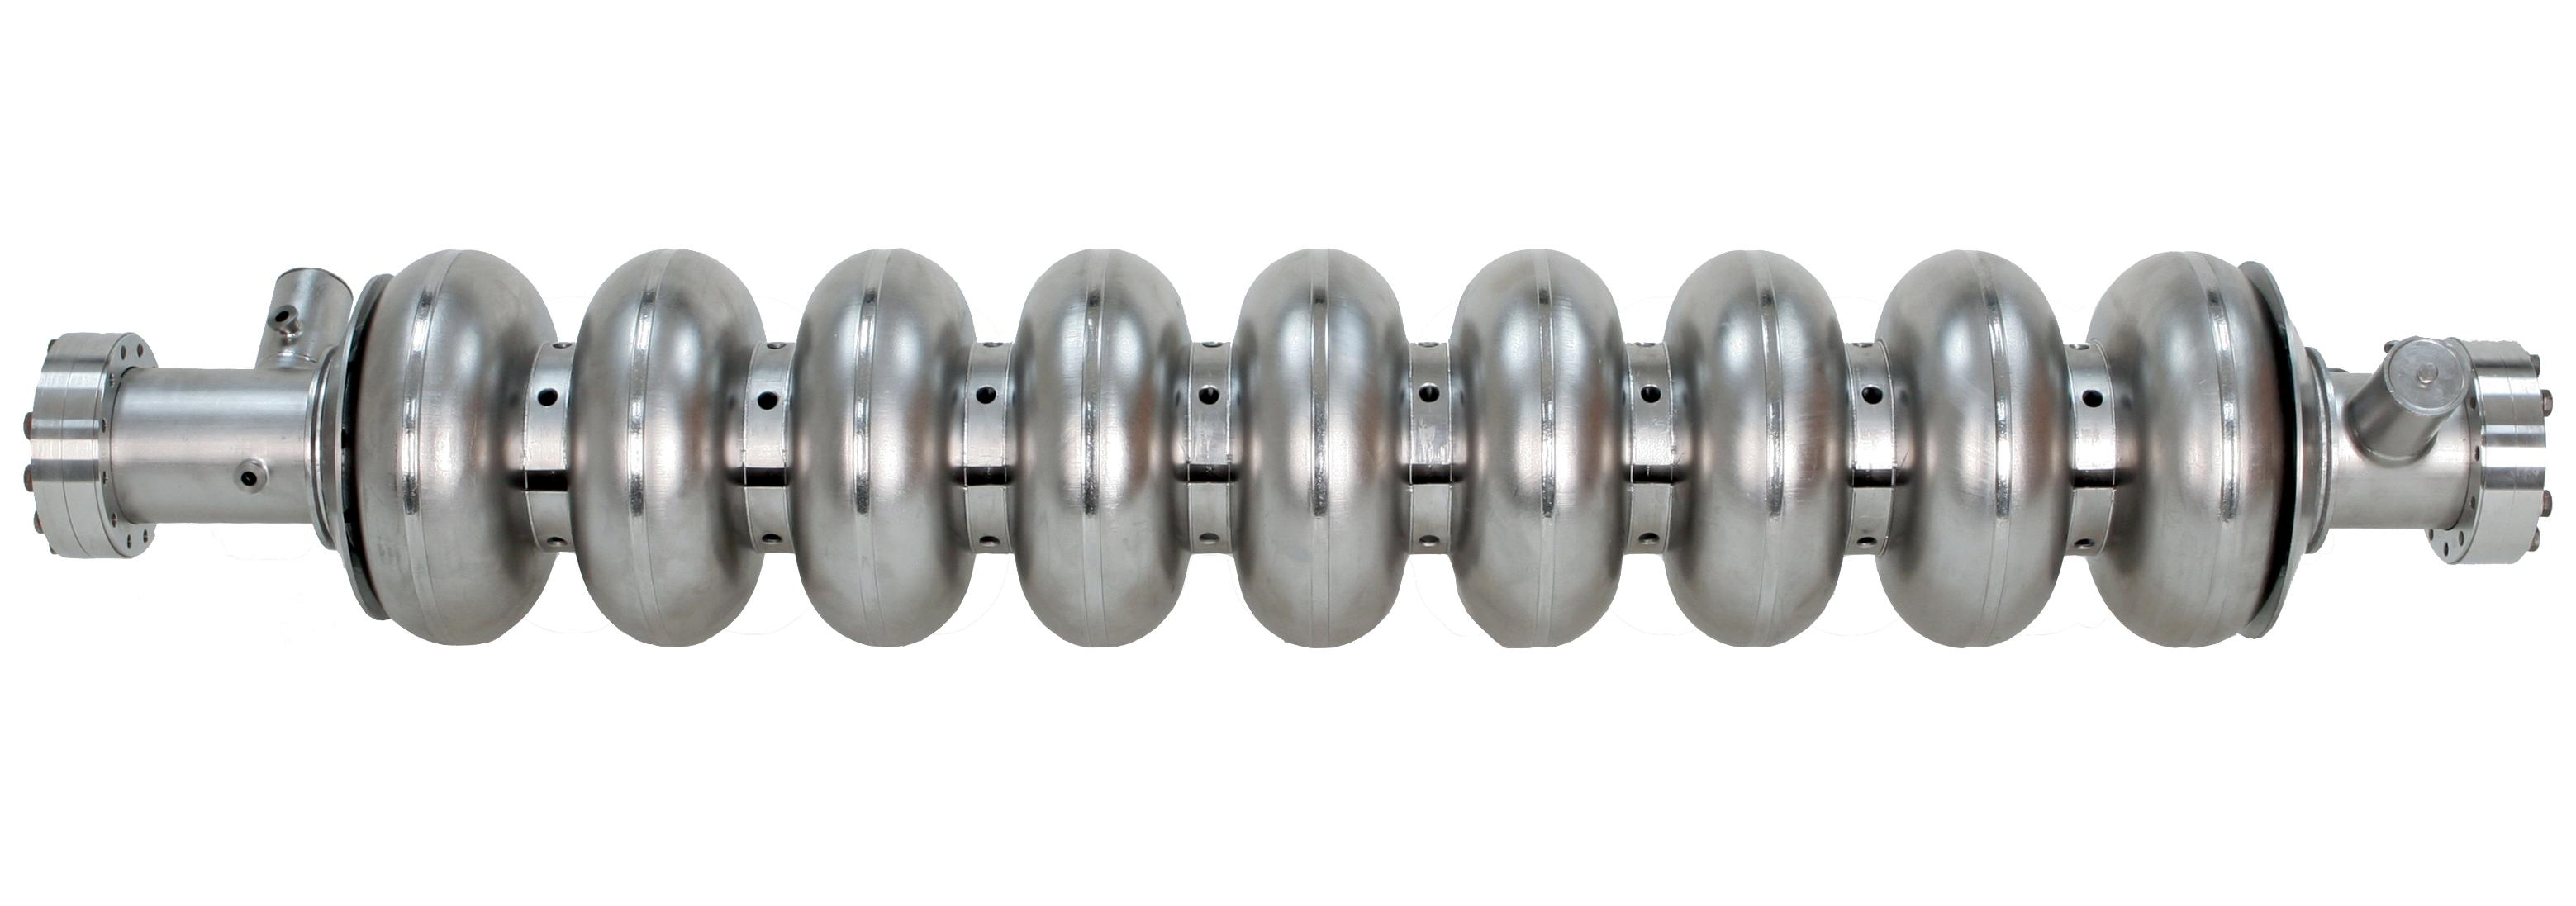
\includegraphics[width=0.95\textwidth]{graphics/Cavity.jpg}
    \caption{\sl External view of the ILC SCRF cavity.}
    \label{fig:ILCcavity}
  }
\end{figure}

\textit{The beam delivery system} is responsible for transporting electrons and positrons from the main high-energy linacs to the interaction point (IP). These systems monitor and focus the electron and positron beams to meet the luminosity requirements and after the collision it transports the residual particles to the beam dumps. 
The beams cross each other at 14\,mrad angle, which provide enough space to separate extraction lines. 

The design of ILC detector hall and beam delivery systems allow hosting of two experiments, SiD and ILD, sharing one interaction point using a push-pull approach. 
%Both detectors are designed as multi-purpose detectors, developed for a wide physics program. 

        \begin{landscape}
        \begin{table}
        \begin{center}
        \begin{tabular}{|lcc|c|c|c|c|c|c|}
                \hline
                Center-of-mass energy &$\sqrt{s}$ &GeV  			& 250 & 350 & 500 & upgrade 1000 \\ 
                Collision rate &$f_{\text{rep}}$ &Hz  				& 5 & 5 & 5 & 4 \\ 
                Electron linac rate &$f_{\text{linac}}$ &Hz  		& 10 & 5 & 5 & 4 \\ 
                Number of bunches &$n_b$ &							& 1,312 & 1,312 & 1,312 & 2450 \\ 
                Bunch population &$N$ &$\times 10^{10}$ 			& 2 & 2 & 2 & 1.74 \\ 
                Main linac average gradient &G$_{\text{av}}$ &MV/m  & 14.7 & 21.4 & 31.5 & 38.2 \\  \hline

                RMS bunch length &$\sigma_{\text{z}}$ &mm 			& 0.3 & 0.3 & 0.3 & 0.25 \\ 
                Electron RMS energy spread &$\Delta p/p$ &\%  		& 0.19 & 0.16 & 0.12 & 0.08 \\ 
                Positron RMS energy spread &$\Delta p/p$ &\%  		& 0.15 & 0.1 & 0.07 & 0.04 \\ 
                Electron polarization &$P_-$ &\%  					& 80 & 80 & 80 & 80 \\ 
                Positron polarization &$P_+$ &\%  					& 30 & 30 & 30 & 20 \\ 
                IP RMS horizontal beam size &$\sigma_{\text{x}}*$ &nm& 729 & 683 & 474 & 481 \\ 

                %(without traveling focus)  &&& & & & \\
                IP RMS vertical beam size &$\sigma_{\text{y}}*$ &nm  & 7.7 & 5.9 & 5.9 & 2.8 \\ \hline
                Luminosity &$\mathcal{L}$ &$\times 10^{34}$\,cm$^{-2}s^{-1}$ & 0.75 & 1.0 & 1.8 & 3.6 \\ 
                Fraction of luminosity in top 1\% &$\mathcal{L}_{0.01}/\mathcal{L}$ & & 87.1\% & 77.4\% & 58.3\% & 59.2\% \\ 
                Average energy loss &$\delta E_{\text{BS}}$&  & .97\% & 1.9\% & 4.5\% & 5.6\% \\  \hline
				Number of pairs per bunch crossing &$N_{pairs}$ &$\times 10^3$ & 62.4 & 93.6 & 139.0 & 200.5 \\ 
                Top pair energy per bunch crossing &$E_{pairs}$ &TeV & 46.5 & 115.0 & 344.1 & 1338.0 \\ \hline
        \end{tabular}
        \end{center}
        \caption{Parameters of the ILC, as given in~\cite{bib:ILC}. }
        \label{tab:ILCparam}
        \end{table}
        \end{landscape}

%%%%%%%%%%%%%%%%%%%%%%%%%%%%%%%%%%%%%%%%%%%%%
%%%%%%%%%%%%%%%%%%%%%%%%%%%%%%%%%%%%%%%%%%%%%
%%%%%%%%%%%%%%%%%%%%%%%%%%%%%%%%%%%%%%%%%%%%%


\subsection{Detector requirements and motivation}

The realization of the ILC physics program requires significant advances in the detector performance. 

%Jet energy resolution
One of the main challenges for detector hardware and reconstruction software is the high-precision jet energy measurement, which is essential, for example, for top mass measurement. This and many other studies require 3-4\%  energy resolution for 100\,GeV jets.
% ---> PFA
The Particle flow algorithms, which are able to reconstruct individual particles inside jets, have been developed to meet this requirement. 
% ---> SiW ECAL
A successful implementation of this technique needs a highly granular electromagnetic and hadron calorimeters.
%The Particle flow technique also requires thick calorimeters for full electromagnetic and hadron shower absorption.

% Charged track resolution 
The Higgs recoil mass measurement using the $e^+e^- \to Z^0H$ process, requires high precision measurements of charged tracks, left by lepton pair from $Z^0$ boson decay. The goal for tracking subdetectors and magnetic solenoid is a momentum resolution for charged tracks $\Delta p/ p^2 \approx 5 \cdot 10^{-5}$\,GeV$^{-1}$.

% Impact parameter resolution
In particular, the reconstruction of the top and the Higgs decays into $b$-quark and $c$-quark pairs, require a high-precision measurement of the track impact parameters by vertex detectors. 
%To achive the targeted flavour tagging performance, 
The required impact parameter resolution depending on track momentum $p$ and track polar angle $\theta$ should be $\sigma_b < 5  \oplus 10/p/\sin^{4/3}\theta$\,$\mu$m.

% ---> Low material deposit
To fit these requirements, all tracking devices should have minimal material budget to minimize multiple scattering, therefore, lightweight detectors, such as thin silicon or gaseous readout devices are preferred.

% Power pulsing
The ILC beam parameters allow for powering off many detector subsystems between bunch trains, introduced in Sec.~\ref{sec:ILCacc}, which reduces heat production and need for active cooling. This method is called power pulsing, and allows reducing the insensitive volumes and reduce material budget for inner trackers, which could be taken by active cooling systems. 

%%%%%%%%%%%%%%%%%%%%%%%%%%%%%%%%%%%%%%%%%%%%%
%%%%%%%%%%%%%%%%%%%%%%%%%%%%%%%%%%%%%%%%%%%%%
%%%%%%%%%%%%%%%%%%%%%%%%%%%%%%%%%%%%%%%%%%%%%

\subsection{The International Large Detector}


The International Large Detector (ILD) is a concept for a high precision multi-purpose detector, designed to meet the ILC physics goals~\cite{Behnke:2013lya}.
%The ILD design is a result of physics driven approach in developing of detector concept by a wide scientific community. 

%The ILD Detector Baseline Design (DBD) is the only approved ILD model within the ILC community, which
The ILD detector baseline design (DBD) is optimized for best resolution and a flexibility towards higher center-of-mass energies up to the TeV range.
The major ILD subdetectors, ordered by their radial distance from the interaction point, are the following, see Fig.~\ref{fig:ILDScheme}:
\begin{itemize}
\item Vertex Detector (VXD) and Forward Tracking Disks (FTD) are the innermost detectors of ILD, which serve to measure impact parameters of particles and track reconstruction up to 36$\degres$;
\item Silicon Inner Tracker (SIT) is used to connect track segments from VXD and TPC;
\item Time Projection Chamber (TPC) serves for charge and momentum reconstruction and particle identification
\item External Tracking Detector (ETD) and Silicon External Tracker (SET) provide a connection between tracks and calorimeter energy depositions 
\item A highly granular Silicon Tungsten Electromagnetic Calorimeter (\ecal) is used to measure and tag electromagnetic energy depositions;
\item A highly segmented Hadronic Calorimeter (HCAL) provides reconstruction and identification of hadrons;
\item Superconducting solenoid creates 3.5~T magnetic field;
\item Tail Catcher and Muon Tracker (TCMT) serves for muon identification and hadron energy measurement.
\end{itemize}
The ILD tracking system can measure tracks up to very small polar angles, as shown in Fig.~\ref{fig:ILDcoverage}.


\begin{figure}
\centering
\begin{subfigure}{0.5\textwidth}
    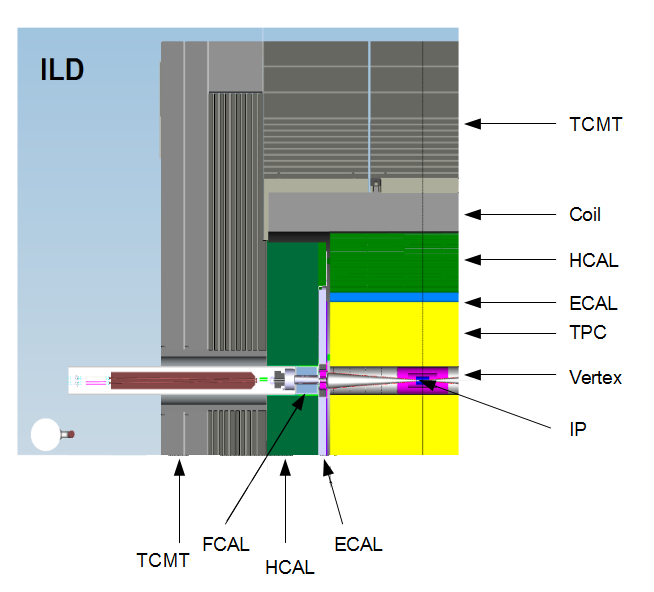
\includegraphics[width=0.95\textwidth]{graphics/ILD.png}

\end{subfigure}% 
  \begin{subfigure}{0.5\textwidth}
\centering
    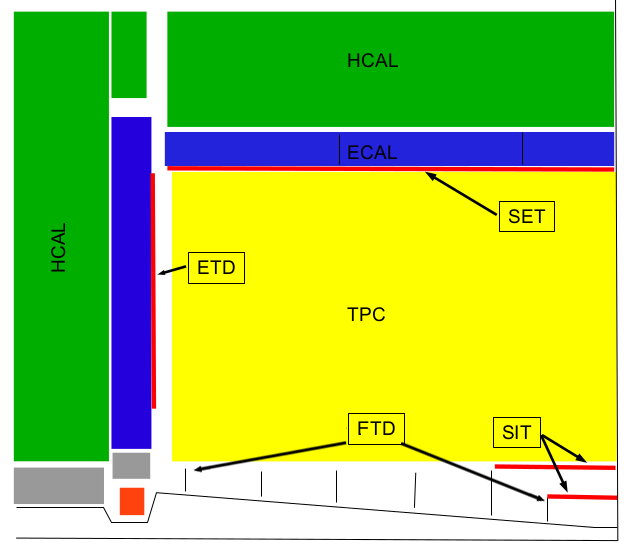
\includegraphics[width=0.9\textwidth]{graphics/ILDtracking.png}

\end{subfigure}
    \caption{\sl Left: Schematic view of the ILD concept. Right: Zoom in the inner detectors.}
    \label{fig:ILDScheme}
\end{figure}


\begin{figure}
	{\centering
		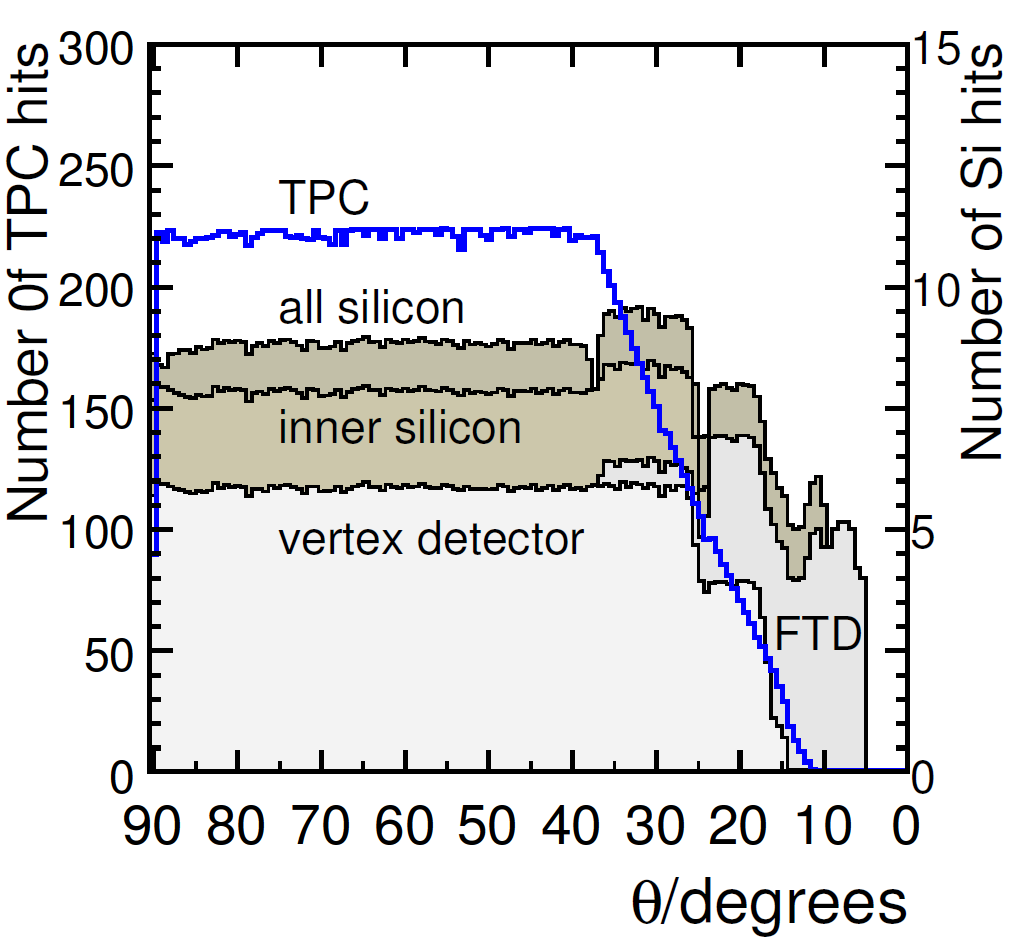
\includegraphics[width=0.45\textwidth]{graphics/ILDcoverage.png}
		\caption{\sl Number of hits as function of track polar angle $\theta$. }
		\label{fig:ILDcoverage}
	}
\end{figure}
%Tracking

% L* models
%However, there are many variations of the baseline model in order to achieve a better physics performance, push-pull synchronization with SiD or cost-performance optimization. 


%%%%%%%%%%%%%%%%%%%%%%%%%%%%%%%%%%%%%%%%%%%%%
%%%%%%%%%%%%%%%%%%%%%%%%%%%%%%%%%%%%%%%%%%%%%
%%%%%%%%%%%%%%%%%%%%%%%%%%%%%%%%%%%%%%%%%%%%%
\subsubsection{Particle flow reconstruction technique}
The ILD concept is designed to meet all requirements for application of the Particle Flow Algorithms (PFA) for physics analysis. 

The PFA allows for the reconstruction of individual particles, even inside jets, which significantly improves the jet energy resolution. For each particle, the best-suited detector information is used, i.e. charged particles are measured in the trackers, and neutral particles are measured in the calorimeters.%, by relying on information from inner tracker and calorimeters.
These algorithms output Particle Flow Objects (PFO), that are reconstructed using hits in the tracking devices and calorimeters. 

\begin{figure}
{\centering
    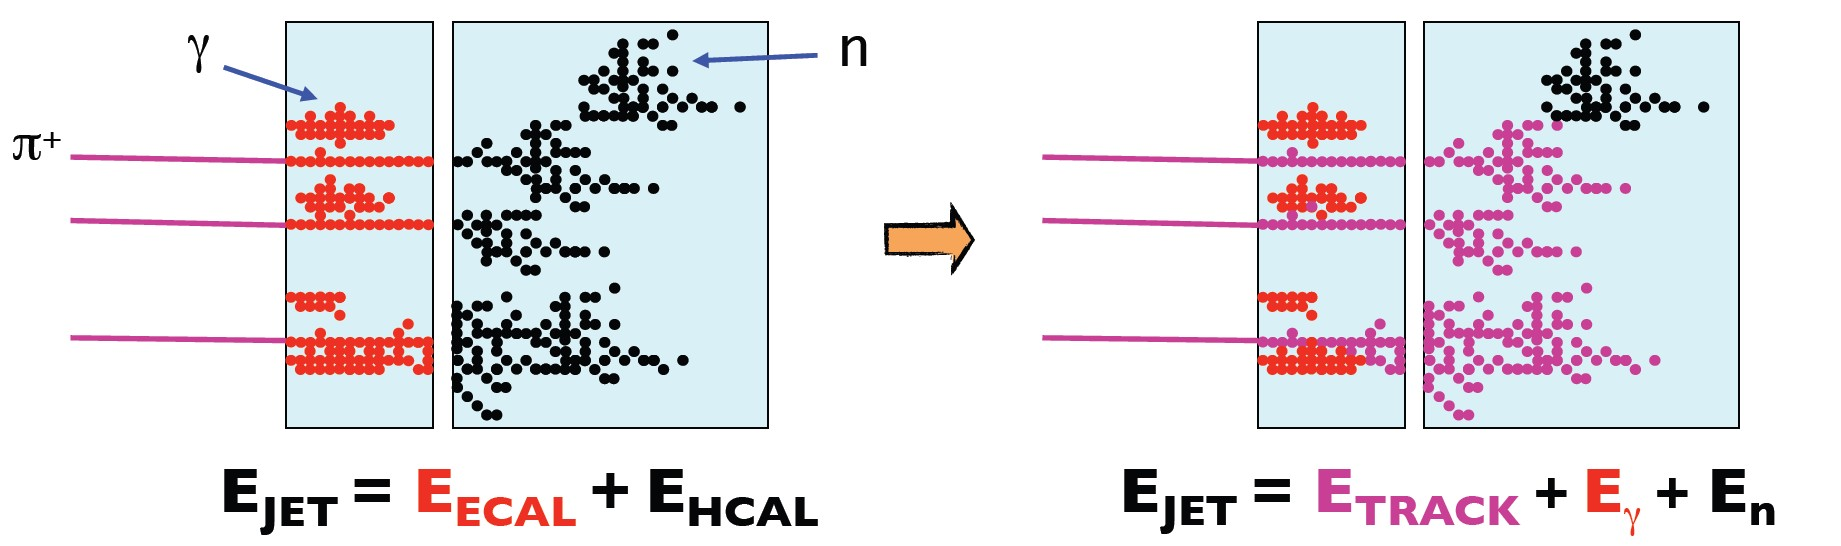
\includegraphics[width=0.95\textwidth]{graphics/calirometry_traditional_new.jpg}
    \caption{\sl Left: Illustration of a jet energy estimation, which is based only on the calorimeter information. Right: Illustration of the Particle flow algorithms, which measure jet energy as a sum of charged and neutral particle energies.}
    \label{fig:PFAillustration}
  }
\end{figure}
%Tracking

First stage of the PFO formation is an individual track reconstruction using tracker information. Tracks have the form of a helix, as a consequence of magnetic field influence on charged particles.  The most common algorithm used is Kalman Filter~\cite{bib:KalTest}.
%clusterization
Then, the energy depositions in the ECAL and HCAL are organized into topological clusters, which are grouped into showers, that correspond to the individual interactions of final-state particles. 
In the general case, the showers, left by hadrons, differ from photon or electron clusters. %The granularity of the calorimeter plays an essential role in the clusterization process. 
High-granular calorimeters are able to separate close-by energy depositions, left by different particles. The illustration of Particle flow process is given in Fig.~\ref{fig:PFAillustration}.

Typically, the PFA creates objects of the following types:
\begin{itemize}
\item Muons have a reconstructed track and track-like energy depositions in ECAL and HCAL, and hits in TCMT;
\item Photons have a compact cluster in ECAL without a connected track;
\item Electrons are reconstructed as a compact cluster in ECAL with an associated track;

\item Neutral hadrons (neutrons, neutral kaons, etc.) appear as a hadronic cluster, that can start in the ECAL or HCAL and continues to TCMT;
\item Charged hadrons (protons, charged kaons, etc.) appear as track, connected to an hadronic cluster.
\end{itemize}

After creating PFOs, one can apply different algorithms like vertex detection, jet clustering, particle identification, flavor-tagging algorithms, etc.

One of the fundamental characteristics of the PFA performance is the jet energy resolution shown for the ILD concept in Fig.~\ref{fig:ILCjetrms}. This plot demonstrates that the detector model is able to meet the requirement of 3-4\% jet energy resolution.

\begin{figure}[H]
{\centering
    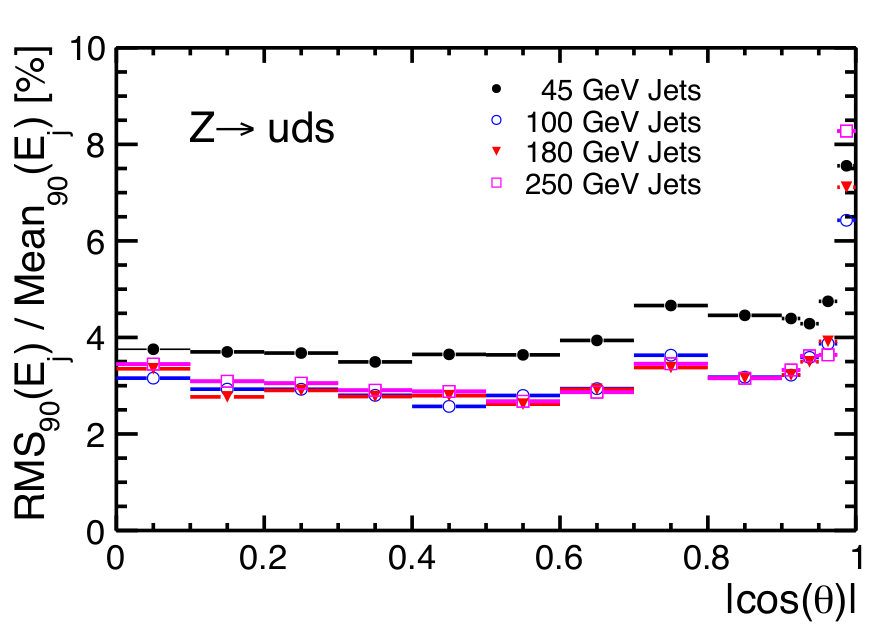
\includegraphics[width=0.55\textwidth]{graphics/ILCjetrms.png}
    \caption{\sl Fractional jet energy resolution plotted versus $|\cos\theta|$ where $\theta$ is the polar angle of the thrust axis of the event. Figure taken from~\cite{bib:ILC}.}
    \label{fig:ILCjetrms}
  }
\end{figure}


%The PFA technique was successfully applied in CMS experiment at LHC.% CMS

%%%%%%%%%%%%%%%%%%%%%%%%%%%%%%%%%%%%%%%%%%%%%
%%%%%%%%%%%%%%%%%%%%%%%%%%%%%%%%%%%%%%%%%%%%%
%%%%%%%%%%%%%%%%%%%%%%%%%%%%%%%%%%%%%%%%%%%%%

\subsubsection{Vertex Detector}
The primary purpose of the ILD Vertex Detector is the precise position measurement of charged tracks aimed at the primary interaction point (IP) and the secondary vertex reconstruction.
%The Vertex Detector of ILD serves to reconstruct position of primary interaction point (IP) and detect tracks with an offset to the IP and organize them into secondary or ternary vertices. 
The secondary vertices are created by particles with a relatively short lifetime, like B mesons, D mesons or $\tau$ leptons. These particles appear in the decay modes of the Higgs boson or the top quark. Therefore, the accurate measurement of track offsets, efficient tagging of $b$- and $c$-quark jets is essential for the top quark and the Higgs physics program. %Another important role of VXD is to reject beam background particles, which requires fast timing of readout devices.

To fulfill the required precision, the VXD is designed to have its first layer at 16\,mm radius from the IP, $\sim 3\,\mu$m single point resolution and a low material budget of the device. To avoid installation of a liquid cooling, the ILD Vertex Detector should also have a low power consumption.

The baseline design of VXD consist of three cylindrical double layers with pixel sensors as readout devices. The VXD layer characteristics are given in Table~\ref{table:ILCvtxparam}.
The VXD layout and its mechanical support is shown in Fig.~\ref{fig:ILCvtxsupport}. 

        \begin{table}[H]
        \begin{center}
        \begin{tabular}{l c c c c c}
        \hline
        			& $R$ (mm) & $|z|$ (mm) & $|\cos\theta|$ & $\sigma$ ($\mu$m) & Readout time ($\mu$m)\\
        \hline
            Layer 1 & 16 & 62.5 & 0.97 & 2.8 & 50 \\
            Layer 2 & 18 & 62.5 & 0.96 & 6 & 10 \\
        \hline
            Layer 3 & 37 & 125 & 0.96 &  4 & 100 \\
            Layer 4 & 39 & 125 & 0.95 &  4 & 100 \\
        \hline
            Layer 5 & 58 & 125 & 0.91 &  4 & 100 \\
            Layer 6 & 60 & 125 & 0.9 &   4 & 100 \\
        \hline
        \end{tabular}
        \end{center}
        \caption{\sl Parameters of the ILC vertex detector system, as given in~\cite{bib:ILC}. }
        \label{table:ILCvtxparam}
        \end{table}

\begin{figure}
\centering

    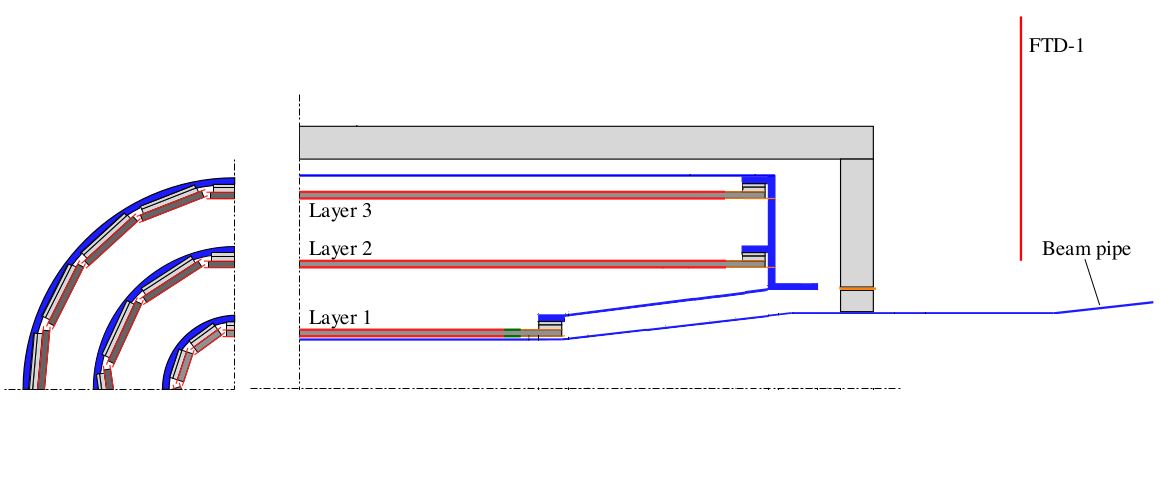
\includegraphics[width=0.9\textwidth]{graphics/ILCvtxsupport.png}
    \caption{\sl Mechanical support structure of ILD vertex detector.}
    \label{fig:ILCvtxsupport}


\end{figure}

Currently, three readout device technology are considered: CMOS Pixel Sensors (CPS), Fine Pixel CCD (FPCCD) and Depleted Field Effect Transistor (DEPFET).
All three technologies are able to provide sensors with up to 50\,$\mu$m thickness and a timing resolution of $\leq 10\mu$s. 

%%%%%%%%%%%%%%%%%%%%%%%%%%%%%%%%%%%%%%%%%%%%%
%%%%%%%%%%%%%%%%%%%%%%%%%%%%%%%%%%%%%%%%%%%%%
%%%%%%%%%%%%%%%%%%%%%%%%%%%%%%%%%%%%%%%%%%%%%

\subsubsection{Forward Tracking Disks}

The ILD forward tracking region consists of seven tracking disks placed between the beam pipe and the TPC. The first two are equipped with pixel sensors to provide a good impact parameter resolution, the other five disks feature silicon strips as readout devices and serve for momentum and charge reconstruction. The layout of the Forward Tracking Discs is summarized in Table~\ref{table:ILCftdparam}. 

        \begin{table}[H]
        \begin{center}
        \begin{tabular}{l c c c c c }
        \hline
        			& $R$ (mm) & $|z|$ (mm) & $|\cos\theta|$ & $\sigma$ ($\mu$m) & Material (\%)\\
        \hline
            Layer 1 & 39-164 & 220 &  0.985-0.802 &  & 0.25-0.5 \\
            Layer 2 & 50-164 & 371 &  0.991-0.914 & 3-6 & 0.25-0.5 \\
        \hline
            Layer 3 & 70-308 & 645 &  0.994-0.902 &   & 0.65 \\
            Layer 4 & 100-309 & 1046 & 0.994-0.959 &   & 0.65 \\
            Layer 5 & 130-309 & 1447 & 0.995-0.998 &  7.0 & 0.65 \\
            Layer 6 & 160-309 & 1848 & 0.996-0.986 &    & 0.65 \\
            Layer 7 & 190-309 & 2250 & 0.996-0.990 &    & 0.65 \\
        \hline
        \end{tabular}
        \end{center}
        \caption{\sl Parameters of ILD Forward Tracking Disks system, as given in~\cite{bib:ILC}. }
        \label{table:ILCftdparam}
        \end{table}

%The main challenges of the FTD are 
The solenoidal magnetic field has a reduced influence on particles in the ILD forward region.
Thus, a precise momentum measurement requires a low material budget and large lever arm. Even small amount of material before the first sensitive layer can compromise the impact parameter precision. To achieve the required performance, first two inner disks featureg high-granular pixels with around 3\,$\mu$m resolution with a minimal material budget. As for the vertex detector, the similar technologies of readout devices are considered: CPS, FPCCD and DEPFET. Outer disks are equipped with AC coupled p-on-n fine-pitch microstrip silicon sensors.
%%%%%%%%%%%%%%%%%%%%%%%%%%%%%%%%%%%%%%%%%%%%%
%%%%%%%%%%%%%%%%%%%%%%%%%%%%%%%%%%%%%%%%%%%%%
%%%%%%%%%%%%%%%%%%%%%%%%%%%%%%%%%%%%%%%%%%%%%

\subsubsection{Time Projection Chamber}

%The ILD central tracker is required to have low material budget, high precision, good timing resolution and have enough points for track reconstruction.
The Time Projection Chamber was chosen as the central tracker of the ILD concept. %is the device, which fulfills all these requirements. 

The TPC consist of an endplate, where the readout of the amplified signals takes place using custom-designed electronics, and a fieldcage, made from advanced composite materials. 
Charged particles, that enter the TPC, ionize the gas mixture inside the chamber. Under an influence of an electric field within the fieldscage, the electrons from track ionization drift to a TPC endplate, equipped with detection devices. The TPC can provide up to 224 points per track.
For a given drift length of more than 2 m and a high magnetic field of 3.5 T, the so-called T2K gas mixture (Ar-CF4(3\%)-isobutane(2\%)) is considered~\cite{bib:ILC}.
A general layout of ILD TPC is shown in Fig.~\ref{fig:ILCtpc}. 
\begin{figure}
{\centering
    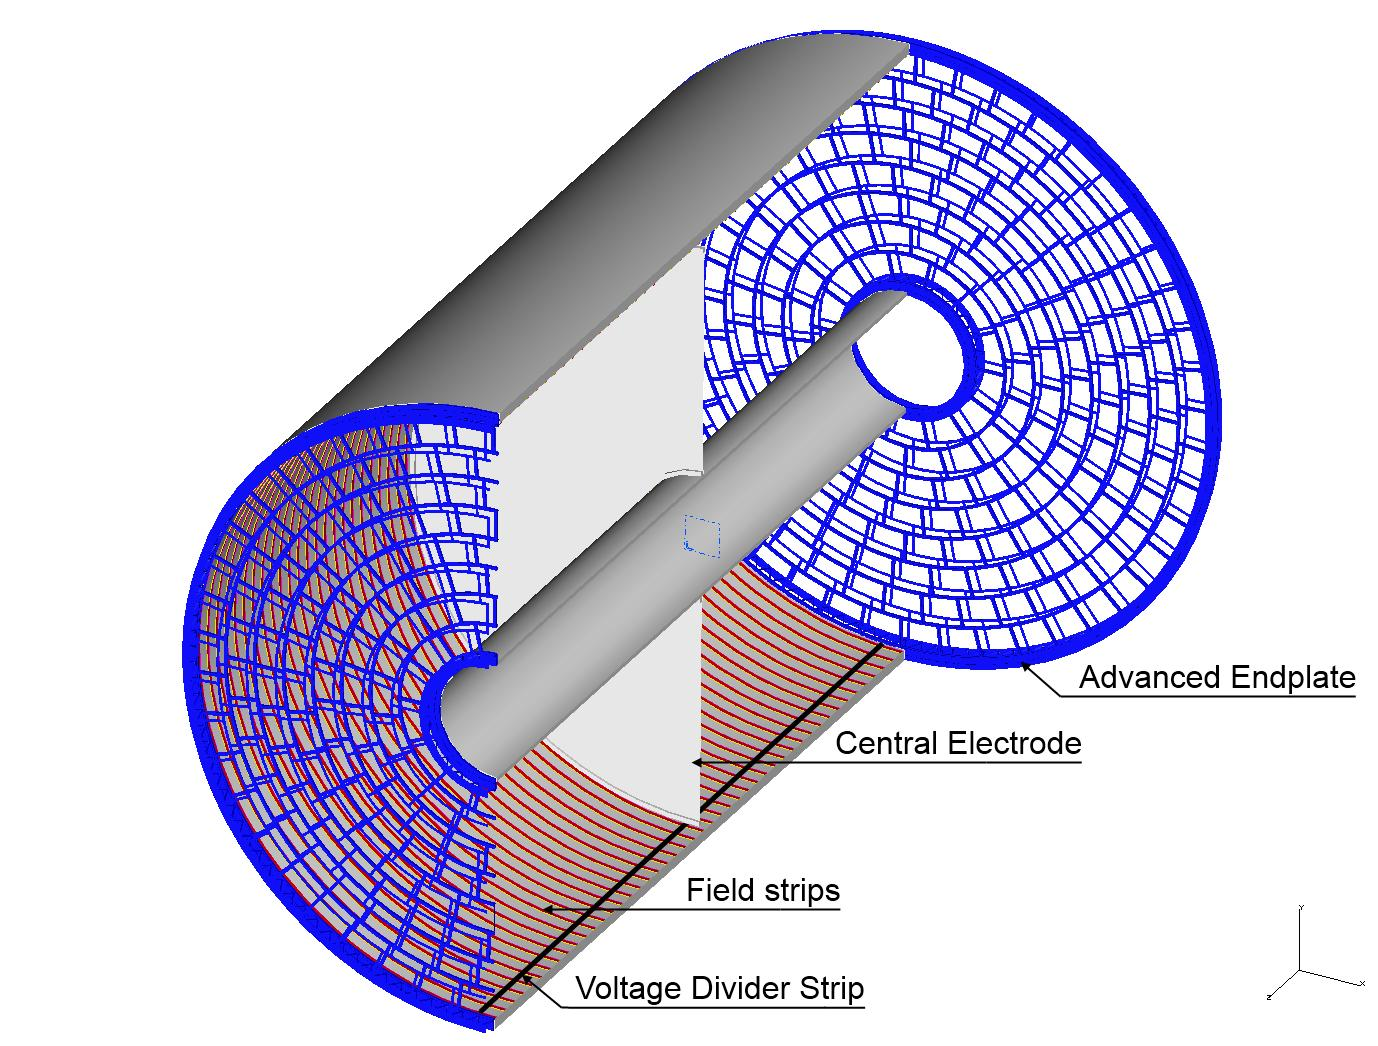
\includegraphics[width=0.55\textwidth]{graphics/ILCtpc.jpg}
    \caption{\sl Scheme of the TPC system showing the main parts of the device.}
    \label{fig:ILCtpc}
  }
\end{figure}	

Currently, Micromegas and Gas Electron Multipliers are considered as detection methods. Both types of detection devices allow measuring the energy deposition per particle track length $dE/dx$, which can be effectively used for particle identification (PID).

A detailed R\&D of TPC for ILD concept is provided by LCTPC collaboration.
%%%%%%%%%%%%%%%%%%%%%%%%%%%%%%%%%%%%%%%%%%%%%
%%%%%%%%%%%%%%%%%%%%%%%%%%%%%%%%%%%%%%%%%%%%%
%%%%%%%%%%%%%%%%%%%%%%%%%%%%%%%%%%%%%%%%%%%%%

\subsubsection{Other tracking detectors}
Silicon Inner Tracker, Silicon External Tracker and External Tracking Detector comprise the Silicon Envelope of ILD and serve for time-stamping, TPC calibration and the track segment synchronization purposes. 
%The general scheme of the system is displayed in Fig.~\ref{fig:ILCtracking}.


The SIT is located between Vertex Detector and TPC. It has two double-sided silicon strip layers, which provide the link between VXD and TPC track segments. ETD and SET are realized with one double-sided layer of silicon strips, which provide a precise entry point of a charged track to the ECAL. All silicon envelope detectors use the same sensor type throughout the system.

The Silicon Envelope of ILD has been developed by the SiLC collaboration.
%%%%%%%%%%%%%%%%%%%%%%%%%%%%%%%%%%%%%%%%%%%%%
%%%%%%%%%%%%%%%%%%%%%%%%%%%%%%%%%%%%%%%%%%%%%
%%%%%%%%%%%%%%%%%%%%%%%%%%%%%%%%%%%%%%%%%%%%%

\subsubsection{Calorimeter System}

The Particle Flow approach drives the calorimeter design. The highly granular calorimeters of ILD can be used not only for a particle energy measurements, but also for a shower separation and particle identification purposes. 
Figure \ref{fig:ILCecal} shows the position of the electromagnetic calorimeter in the ILD detector.

\begin{figure}
	{\centering
		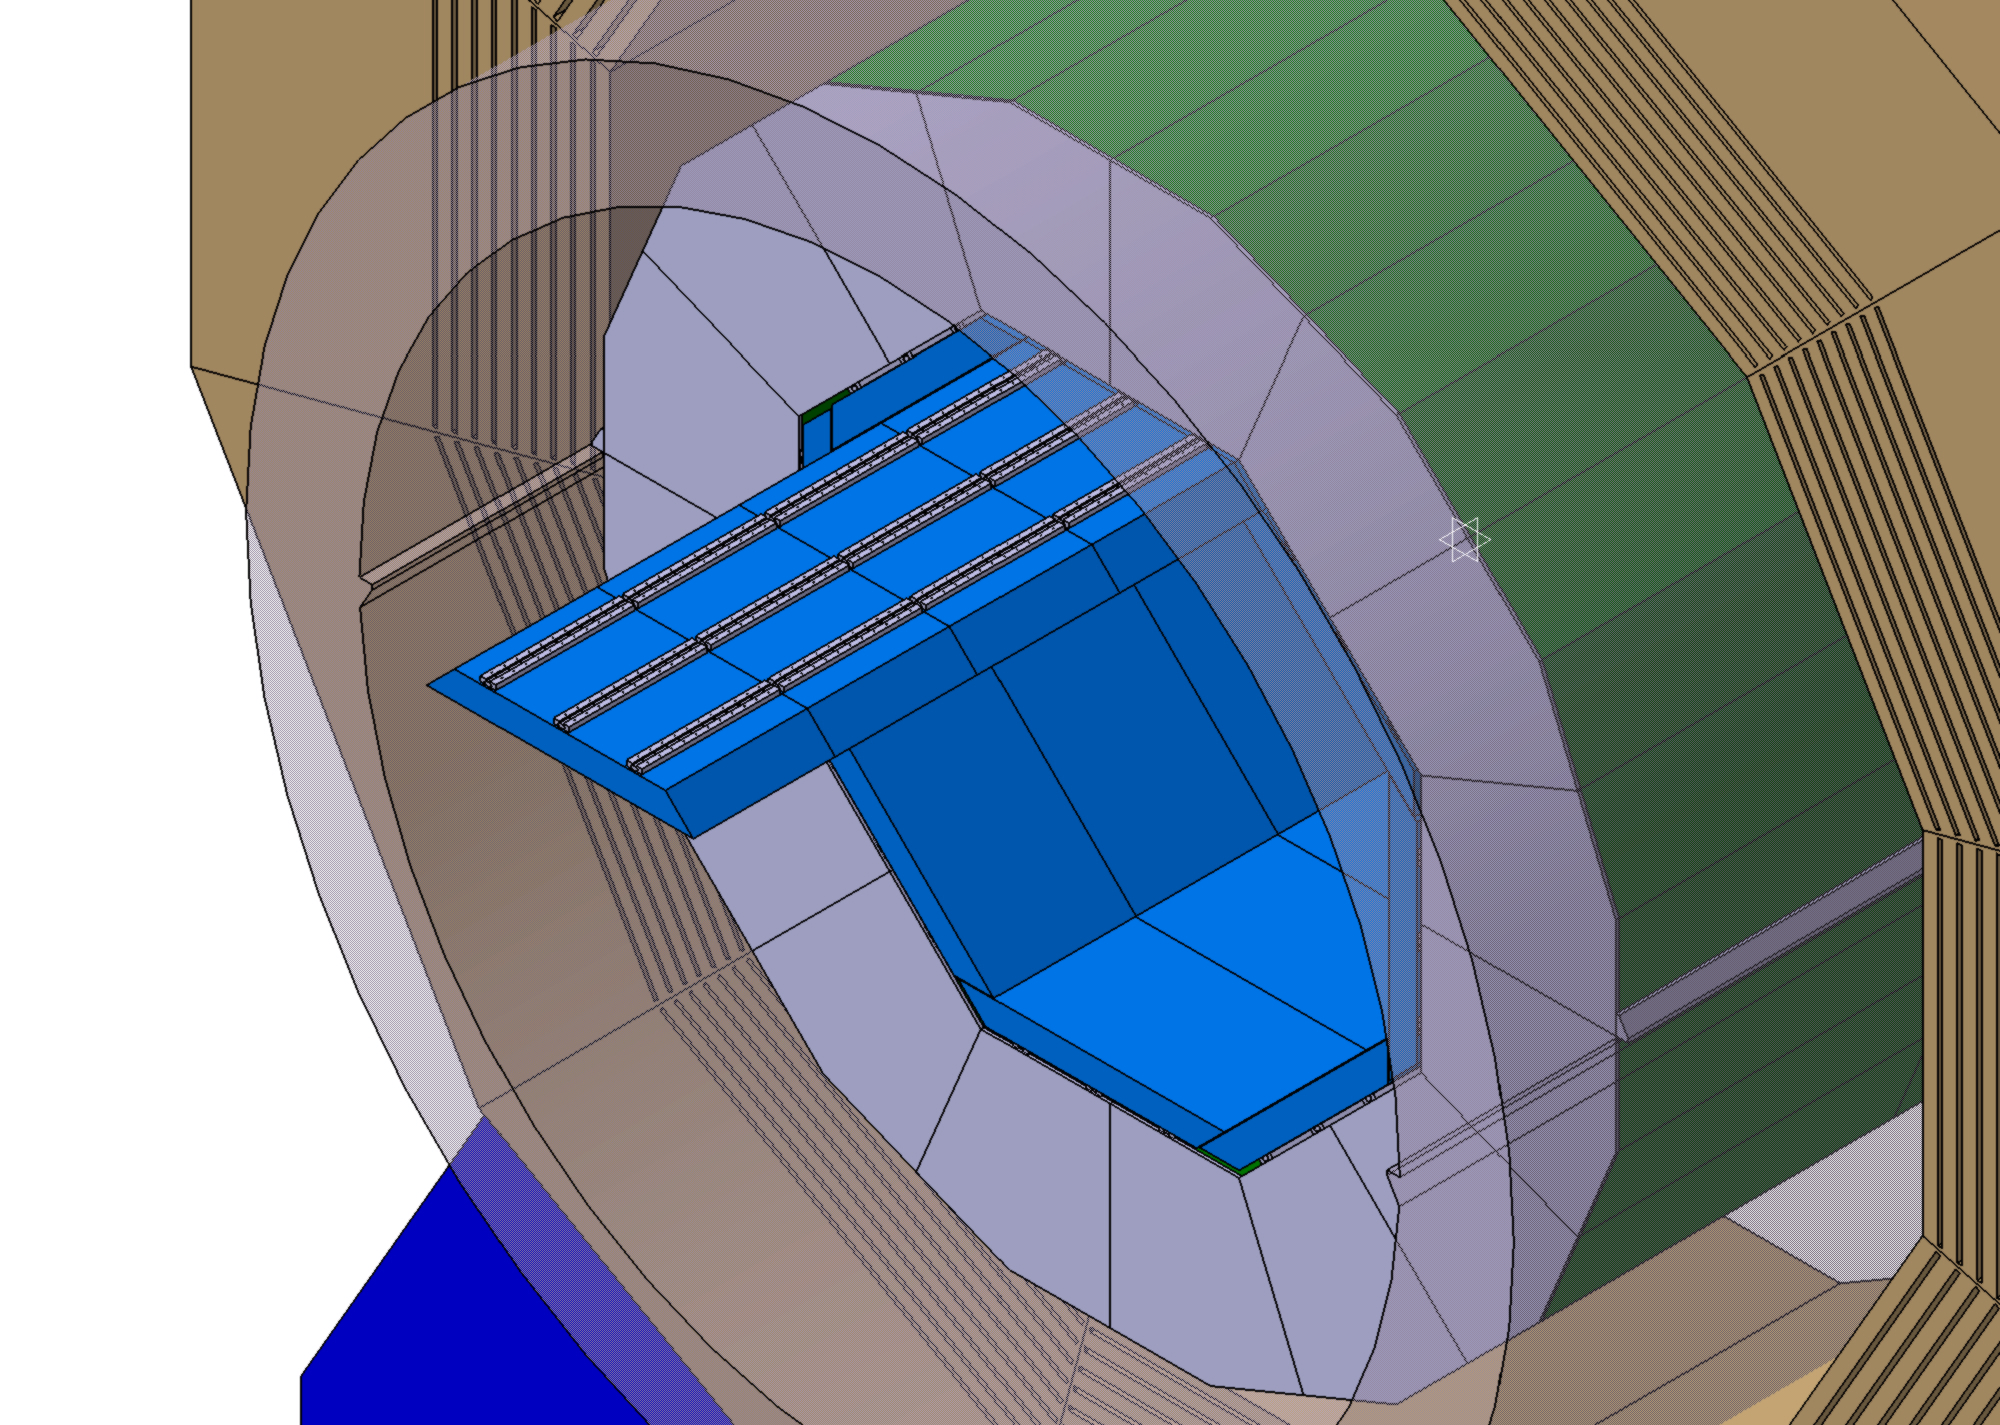
\includegraphics[width=0.55\textwidth]{graphics/ild-cal.png}
		\caption{\sl The electromagnetic calorimeter (in blue) within the ILD Detector~\cite{bib:ILC}.}
		\label{fig:ILCecal}
	}
\end{figure}

The principal role of the ECAL in the PFA framework is photon reconstruction in presence of close-by particles. The device should be able to disentangle electromagnetic showers caused by photons or electrons from hadronic ones. Thus, high granularity in three dimensions is required. For these purposes, the ILD ECAL has a sandwich-like structure of 30 active readout layers with tungsten absorber layers in between. The total thickness of the absorber corresponds to 24 radiation lengths $X_0$ and 1 nuclear interaction length $\lambda$, see Sec.~\ref{sec:Passage}. The readout technology is silicon pin diodes of 5 $\times$ 5\,mm$^2$ size. This device is referred as \ecal. Another option for the readout sensors are scintillator strips with silicon photomultipliers.

The hadronic calorimeter is designed to separate neutral and charged hadrons and precisely measure energy depositions of neutral hadrons. The HCAL has 42 sensitive layers with steel absorber in between. Two baseline readout options are considered, the scintillator-tile based AHCAL and the Glass Resistive Plate Chamber (GRPC) based SDHCAL.

The CALICE collaboration made a detailed R\&D of highly granular calorimeters, constructed and tested prototypes with different readout options. 
\ecal\ prototype by CALICE collaboration is described in Section~\ref{sec:ecal}.

%%%%%%%%%%%%%%%%%%%%%%%%%%%%%%%%%%%%%%%%%%%%%
%%%%%%%%%%%%%%%%%%%%%%%%%%%%%%%%%%%%%%%%%%%%%
%%%%%%%%%%%%%%%%%%%%%%%%%%%%%%%%%%%%%%%%%%%%%

\subsubsection{Outer part}

The outer part of ILD concept consist of superconducting solenoid and muon system / tail catcher. 

The superconducting coil surrounds the ILD calorimeters and creates an axial magnetic field of 3.5~T.

TCMT serves for magnetic flux confinement and, at the same time, it provides a measurement of residual energy depositions of hadronic showers and muon-tagging. Sensitive layers can be either scintillator strips or resistive plate chambers. 



\newpage\part{Hadronic interactions in the Silicon-Tungsten Electromagnetic Calorimeter}\label{PARTII}
\section{Passage of particles through matter}

The main principle of the particle detection in particle physics is the detection via interaction with an ordinary condensed matter. 
The particles can interact with free or bound electrons in matter, or with atomic nuclei. 
The study of high-energy particles is done using the following methods:
\begin{itemize}
	\item Detection and measurement of radiative light emitted while travelling through matter of tracking devices;
	\item High-energy photons or electrons in thick absorbers initiate electromagnetic cascades or showers, which are measured in electromagnetic calorimeters;
	\item High-energy hadrons interact with matter nuclei via strong force creating  hadronic cascades, measured by hadronic calorimeters.
\end{itemize}
%Different regimes of energy losses
\subsection{Electronic energy losses}
The radiated photons by energetic charged particles lead to ionization, atomic, or collective excitation in ordinary matter. 
The mean rate of energy loss per unit of length $<-dE/dx>$ by relativistic massive particles is described by Bethe-Bloch formula~\cite{bib:PDG}. 
This equation depends on the particle charge and momentum, as well as on the matter properties, such as atomic mass and atomic number. 
As an example, the energy loss of muons on copper target as function of particle momentum is demonstrated in Fig.~\ref{fig:BB_2}.
For the studies presented in this thesis, the relevant energy range is from 100\,MeV up to 100\,GeV, which is the minimal energy loss region in Fig.~\ref{fig:BB_2}.
The particles with a momentum corresponding to the minimun of the  $<-dE/dx>$ curve are called minimum ionizing particles or MIPs. 
\begin{figure}
	\centering
	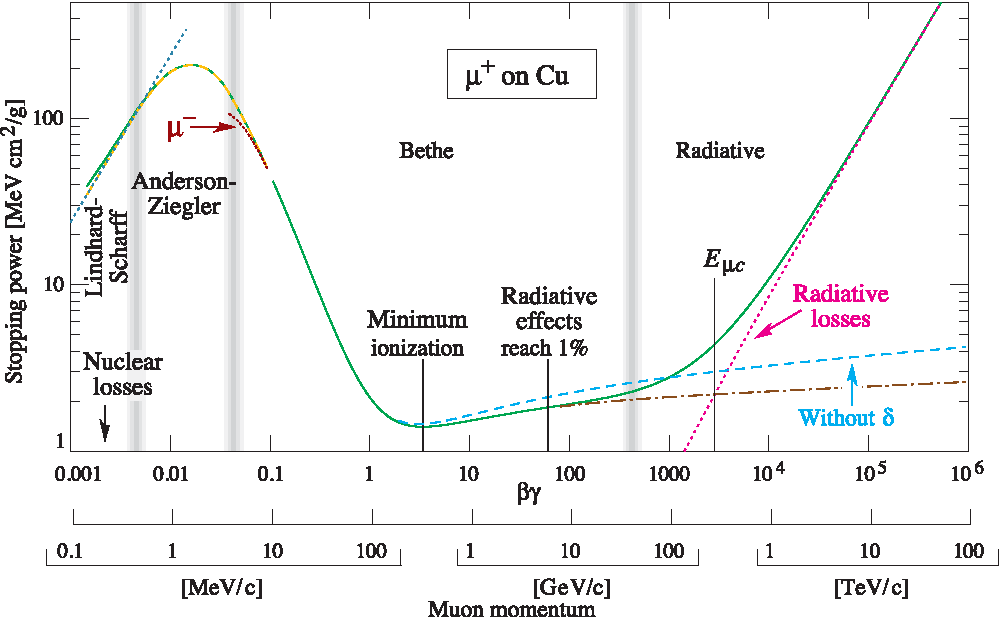
\includegraphics[width=0.95\textwidth]{ECAL/graphics/rpp_icru49_cu.pdf}
	\caption{\label{fig:BB_2} \sl Stopping power or $<-dE/dx>$  for muons in copper as a function of $\beta\gamma = p/mc$, where $m$ is the muon mass, $p$ is muon momentum and $c$ is the speed of light. }
\end{figure}
\subsection{Electromagnetic showers}
The emission of photon or bremsstrahlung process is the dominant process of the energetic electron-matter and positron-matter interaction.
The high-energy photons interact with matter via the convertion to $e^+e^-$ pair.
Thus, passage of these particles in dense materials create an intense cascade of pair creation and photon radiation processes, i.e. electromagnetic cascades or showers.
Eventually, the electron energy falls below the critical energy of the bremsstrahlung, and then they lose their energy by ionization and atomic excitation processes.
Below the $e^+e^-$ pair convertion threshold, the photons lose their energy in the material by the Compton scattering process. 

The main characteristic of the material is the radiation length $X^0$, defined as the mean distance over which a high-energy electron loses all but $1/e$ of its energy, or $7/9$ of the mean free path of a high-energy photon. 
The transverse size of the electromagnetic cascade is described by Moli\`ere radius $R_{m}$, which is defined as an average radius of a cylinder containing 90\% of an electromagnetic cascade. Moli\`ere radius is proportional to the radiation length of the material. 
The radiation length and the Moli\`ere radius values for various materials are shown in Table~\ref{table:material}.
        \begin{table}[H]
        \begin{center}
        \begin{tabular}{l c c c c}
        \hline
	Material & $X_0$ [cm] & $R_m$ [cm] &  $\lambda_{I}$ [cm] & $\lambda_{\pi^{\pm}}$ [cm]  \\
	\hline
	Dry air  & 30390 & 7330 & 74770 & 101300 \\
	Iron Fe  & 1.757 & 1.719 & 16.77 & 20.42 \\
	Lead  Pb & 0.5612 & 1.602 & 17.59 & 19.93 \\
	Tungsten W &0.35&0.93& 9.946 & 11.33 \\ 
        \hline
        \end{tabular}
        \end{center}
        \caption{\sl The material properties of interest for high-energy physics~\cite{bib:PDGprop}. }
        \label{table:material}
        \end{table}


\subsection{Hadronic showers}
All hadrons have an electric and a confined color charge. 
Thus, the charged hadrons can interact with material via ionization process, and all hadrons, neutral and charged ones, can interact with matter nuclei via the strong force.
The strong interaction with matter can be elastic and inelastic. 
The elastic hadron-matter interaction is the nucleus excitation process, via gluon exchange, which do not change the hadron or nuclei composition. 
The inelastic hadron-matter interaction often leads to a spallation of the target nuclei creating new stable or unstable hadrons. 
The emitted relatively energetic  $\pi^0$ and $\eta$ mesons decaying into two photons give a rise to an electromagnetic shower. 
The stable and long-lived hadrons, like pions, protons and neutrons, can escape the collision region. 
Thus, the energy deposit value of the hadronic showers is highly fluctuating. 

The material is characterized by the nuclear interaction length $\lambda_{I}$, which is defined as a mean material length reducing the number of passing by hadrons by the factor of $1/e$. 
Specifically, the pion interaction length $\lambda_{\pi^\pm} > \lambda_{I}$, due to longer mean free path of the $\pi^\pm$ in the same type of material. 
The   $\lambda_{\pi^\pm} $ and $ \lambda_{I}$ values for various materials are given in Table~\ref{table:material}.
\subsection{Simulations}
The most famous toolkit to simulate the passage of particles through matter is \geant\ simulation software~\cite{Allison:2006ve}. 
It is used in a variety of application domains, including high energy physics, astrophysics and space science, medical physics and radiation protection. 
The \geant\ physics processes cover variety of particle-matter interactions over a wide energy range.
The description of highy-fluctuating processes, like hadron-matter interaction, can be done by using different approximations. 
Thus, simulation of the hadron-matter interaction in \geant\ is implemented in physical models called \textit{physics lists}~\cite{bib:G4pl}.

\section{Introduction}
%General introduction

The design of particle detectors at future high-energy physics experiments and, in particular, at linear colliders is oriented towards the usage of Particle Flow algorithms (PFA) for the event reconstruction. 
These algorithms require calorimeters with high granularity to reconstruct individual particles, aiming at the improvement of the jet energy resolution \cite{Brient:2002gh}. 

The primary objective of the CALICE (Calorimeter for the Linear Collider Experiment) collaboration is the development, construction and testing of highly granular hadronic and electromagnetic  calorimeters for future particle physics experiments.

A detailed study of the calorimeter response to particle interactions is necessary to verify existing Monte Carlo simulation models and to build a reliable PFA. 
This implies the precise simulation and reconstruction of the interaction of neutral and charged hadrons and the subsequent particle cascade.

This note reports on a detailed study of hadronic interactions in the CALICE Silicon-Tungsten Electromagnetic Calorimeter (\ecal) physics prototype \cite{Anduze:2008hq}.
The \ecal\ was tested at Fermi National Accelerator Laboratory (FNAL) in 2008 using a beam of $\pi^-$-mesons in the energy range from 2 to 10\,GeV. 
%High energy jets are predominantly composed of neutral and charged pions within this energy range and therefore the performance of Monte Carlo simulations with these particles is important.
The highly granular structure of the \ecal\ permits a detailed measurement of hadronic showers in terms of integral observables \cite{Bilki:2014uep} such as cluster extensions and energy depositions. As will be shown in this note, the high granularity allows in addition for deeper studies of the interactions between the hadrons and the absorber material such as the characterisation of the interaction region and the analysis of secondaries emerging from the interaction. The tracks produced by these secondaries are reconstructed by a new simple \tfa . The resulting observables are subject to comparison of data with predictions from different {\sc Geant}4 Monte Carlo physics lists. The analysis complements studies presented in~\cite{Adloff:2013vra} and~\cite{bib:can-047} for tracking in CALICE prototypes of hadronic calorimeters.  

%and differential observables, like kinematics of secondary particles, that emerge from hadron-detector interactions.


%TODO: insert new results of study if any
%This study is done as an extension of Ref. \cite{bib:Naomi}, where Monte Carlo simulation are compared with data using global observables like lateral and longitudinal extension of the hadronic cascade immediately after the first interaction.
%and they can create energy depositions outside a main hadronic showers. 
%The reconstruction of these secondary tracks provides a new set of observables that can:
%\begin{itemize}
%\item extend Monte-Carlo comparison with experimental data by using kinematic observables of secondary particles;
%\item improve reconstruction of the energy of neutral hadrons by detecting distant energy depositions using track information inside calorimeter;
%\item improve Particle ID algorithms by introducing more detailed shower shape information for identification of hadron interaction in the \ecal.
%\end{itemize}
%||||||||||||||||||||||||ECAL|||||||||||||||||||||||%

\section{The \ecalp}
\label{sec:ecal}
The \ecalp\ has a sandwich-like structure comprising 30 layers of silicon (Si) as active material, alternated with tungsten (W) as absorber material. The active layers are made of Si wafers segmented in 1 $\times$ 1\,cm$^2$ pads. As shown in Fig. \ref{fig:ECAL-scheme}, each wafer consists of a square of 6 $\times$ 6 pads and each layer is a matrix of 3 $\times$ 3 of these wafers resulting in an active zone of 18 $\times$ 18\,cm$^2$.
\begin{figure}[H]
	\centering
	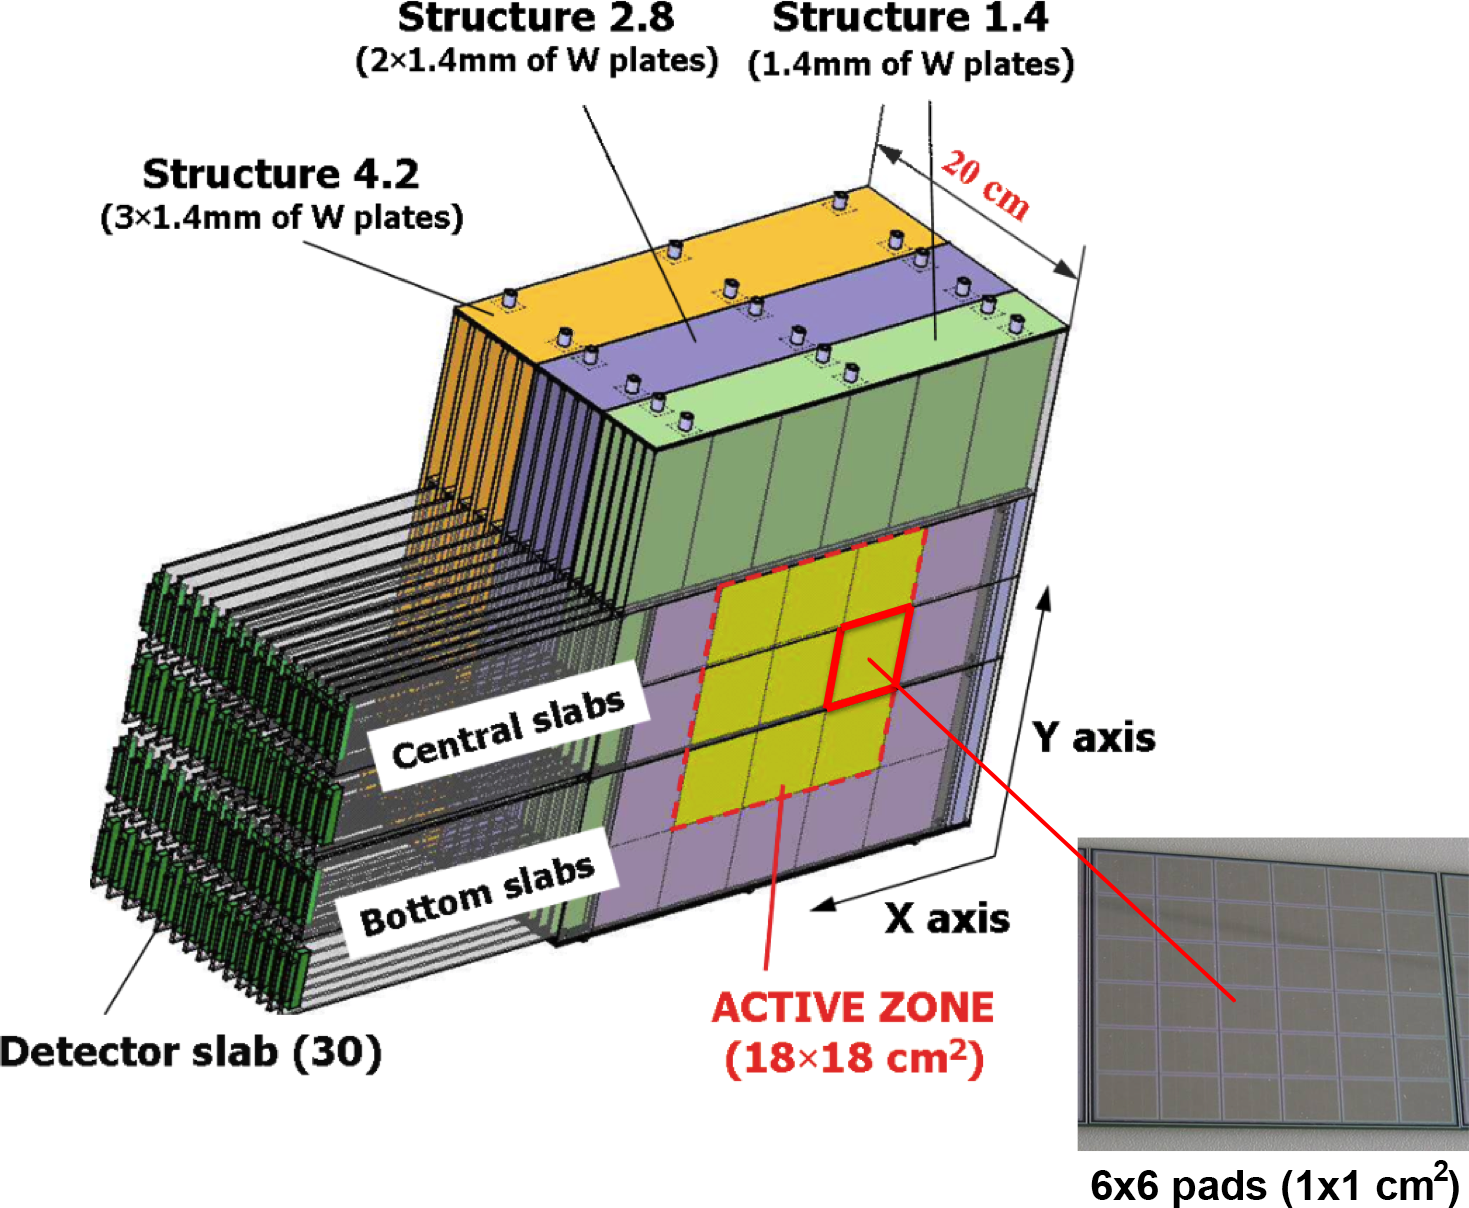
\includegraphics[width=0.5\textwidth]{ECAL/graphics/ecal-new.png}
	\caption{\label{fig:ECAL-scheme} \sl A schematic view of the \ecalp.}
\end{figure}
The \ecal\ is subdivided into 3 modules of 10 layers each. The W depth per layer is different in each module increasing from 1.4\,mm (0.4 radiation lengths or $X_0$) in the first one, to 2.8\,mm in the second and 4.2\,mm in the last one. The total thickness corresponds to 24 $X_0$ or about 1 nuclear interaction length $\lambda_I$ which ensures that more than half of the hadrons will have a primary interaction within the detector volume.
%This frame is used for the clustering and tracking algorithm, described in Sec. \ref{sec:track}.
%The direction of $z$-axis is parallel to the primary particle momentum.
A more detailed description of the prototype can be found in \cite{Anduze:2008hq}.

%|||||||||||||||||||Description of a dataset||||||||||||||||||||%

\section{Data and Monte Carlo samples}
\label{sec:data}
\subsection{Experimental setup at FNAL}\label{sec:fnal}
The test beams were carried out at the Fermilab Test Beam Facility\footnote{\label{note1}Fermilab Test Beam Facility web page: \url{http://www-ppd.fnal.gov/MTBF-w}}, FTBF, at FNAL in May and July 2008.
The \ecal\ was placed in front of two other CALICE physics prototypes: an AHCAL \cite{collaboration:2010hb} and a TailCatcher (TCMT) \cite{CALICE:2012aa}.
The beam-line comprised in addition two scintillator counters, covering an area of 10 $\times$ 10 cm$^2$, for triggering on incoming particles and two Cherenkov detectors for particle identification.
The chosen coordinate system is right-handed with the $z$-axis pointing along the beam direction and the $y$-axis being vertical.
The analysed data in this note comprise runs with primary $\pi^-$-mesons. The energies of the primary particles are 2, 4, 6, 8 and 10 GeV.

\subsection{Monte Carlo simulations}

%Due to the complicated nature of hadronic interactions a precise description of hadronic showers in simulations is difficult to achieve. 
Monte Carlo simulations were carried out within the Mokka framework~\cite{MoradeFreitas:2002kj}, which provides the geometry interface to {\sc Geant}4~\cite{Allison:2006ve}. 
There are several simulation models of hadronic interactions available within {\sc Geant}4, that are combined into so-called \textit{physics lists}.
Each model has its own theoretical basis valid mainly in a specific energy range of hadrons. In this analysis, three physics lists contained in {\sc Geant4} version 10.01 are compared with the experimental data:
\begin{itemize}
	\item \qgsp\ combines the Bertini model
	at energies below 9.9\,GeV, with the Low Energy Parametrised model at energies above 9.9\,GeV;
	\item \ftfp\ has a transition from the Bertini model to the Fritiof model around a primary particle energy of 4.5\,GeV.
	\item \qbbc also intrapolates between the Bertini model and the Fritiof model however with a larger transition region.
\end{itemize}
The physics lists are illustrated in Fig.~\ref{fig:physicslist_2}.
\begin{figure}
	\centering
	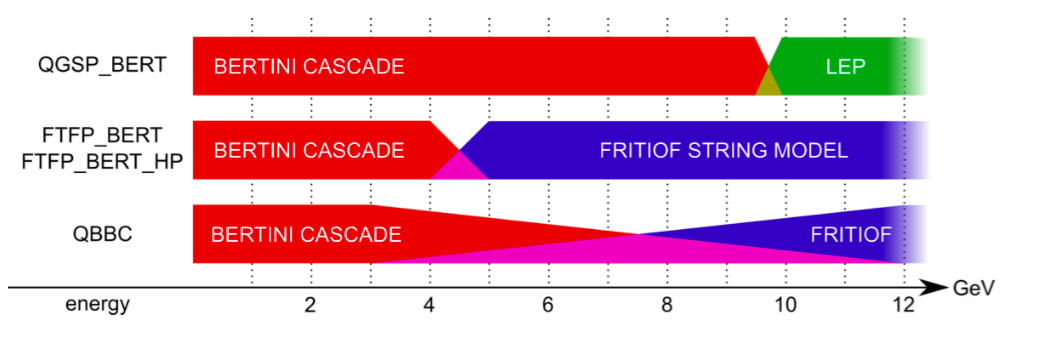
\includegraphics[width=0.95\textwidth]{ECAL/graphics/physics-lists.png}
	\caption{\label{fig:physicslist_2} \sl Illustration of the transitions between the different physics models within the used \geant\ physics lists.  }
\end{figure}
More information about these and other physics lists can be found in \cite{bib:G4pl}.

\subsection{Event selection and preprocessing}

The FNAL $\pi^-$ test beam is contaminated with $\mu^-$ and $e^-$, in particular at lower energies where the beam is dominated by $e^-$. 
At 2 GeV the beam contains about 5\% of $\pi^-$ mesons and 70\% of electrons. 
Events are triggered using the signals from the two scintillator counters upstream of the \ecal\ and $\pi^-$ are identified by using Cherenkov counters.
The response of the \ecal\ to charged particles was calibrated with  an energetic $\mu^-$ beam \cite{li:tel-00430432} and the hit energy is converted into units of most probable energy depositions by minimum ionising particles (MIP). 
%Muons penetrate the whole detector volume with a nearly identical energy loss rate which is minimal for the beam energy used. 
%These $\mu^-$ are so-called minimum ionising particles or MIP and their mean energy loss in the active medium of a pad defines the energy unit MIP.

To select $\pi^-$ showers the data and simulation samples undergo the following selection steps \cite{Bilki:2014uep}\cite{bib:Doublet}: 
\begin{itemize}
	\item A series of cuts is applied to reject multi-particle events caused by beam impurities or products of decays or upstream interactions of primary particles. The influence of residual multi-particle events will be discussed in Sec.~\ref{sec:results};
	\item A threshold of 0.6 MIP is chosen to remove noisy hits in the \ecal;
	\item A hit is removed as being isolated if all the 26 pads in the surrounding cube have no signal above the noise threshold. The analysis presented in this note applies to the non-isolated hits that remain after this removal. The term hits will continue to be used.   
	\item The total number of hits in the ECAL is required to be at least 25 to remove particles with large incident angle;
	\item The barycentres of the transverse coordinates $\bar{x}_{hit}$ and $\bar{y}_{hit}$ of the hits are calculated as:
	\begin{eqnarray}
	\label{eq:barycentre}
	\bar{x}_{hit} = \frac{\displaystyle \sum_{hits} x_{hit}\,E_{hit}}{\displaystyle \sum_{hits} E_{hit}} 
	\text{ and }
	\bar{y}_{hit} = \frac{\displaystyle \sum_{hits} y_{hit}\,E_{hit}}{\displaystyle \sum_{hits} E_{hit}},
	\end{eqnarray}
	where $E_{hit}$ is the energy of a hit in MIP units, and the sums run over all hits in the calorimeter.
	The event is accepted if $-50\,{\rm mm} < \bar{x}_{hit} < 50\,{\rm mm}$ and $-50\,{\rm mm} < \bar{y}_{hit} < 50\,{\rm mm}$ to
	reduce lateral shower leakage;
	\item  In first approach the interaction layer $i$ is identified with the first of three consecutive layers for which
	\begin{equation}
	E_i > E_{cut}, E_{i+1} > E_{cut}  \text{ and } E_{i+2} > E_{cut}.
	\end{equation}
	This simple condition is inefficient at small energies and is complemented by using the following relative energy increase
	\begin{equation}
	\frac{E_i+E_{i+1}}{E_{i-1} + E_{i-2}} > F_{cut} \text{ and } 
	\frac{E_{i+1}+E_{i+2}}{E_{i-1} + E_{i-2}} > F_{cut}, 
	\end{equation}
	with $E_i$ being the total energy of layer $i$. The variables $E_{cut}$ and $F_{cut}$ are free parameters with empirical values of 8 MIP and 6, respectively. It is argued in \cite{Bilki:2014uep} and references therein that these values optimise the selection efficiency in the energy range relevant for the present study.
	The event is selected if $5 < i < 15$ to suppress electron contamination and to assure "long" secondary tracks after the interaction.
	%\item a cut on minimal number of hits in  two last layers of \ecal\ was applied to reduce number of events with elastic scattering.
\end{itemize}
%This selection scheme originally developed and used in \cite{bib:Naomi}\cite{bib:2012_Doublet}.
%Preselect the events, which have an energy deposition at the last layers of the ECal and interaction in the first half of the Ecal

%---------------------------------------------------------------
%----------------------------TFA--------------------------------
%---------------------------------------------------------------

\section{The \tfa}
\label{sec:track}

%\subsection{Algorithm description}
%The outgoing charged secondary particles in hadron interactions leave tracks in the \ecal. 
%These tracks are reconstructed by a  new simple \tfa\. 
%The resulting observables is used for comparison of different {\sc Geant}4 Monte Carlo simulations with experimental data, taken at FNAL in 2008. 
%Identification of tracks in hadronic showers is useful for precise energy calculation in PFA and for more detailed comparison of experimental data and Monte Carlo simulations. 
%The \tfa\ developed here is oriented on a Monte Carlo comparison study for \ecalp\ using new set of observables, based on properties of secondary particles from hadronic interactions. 

The main objective of the \tfa\  is the detection of forward-scattered tracks from the interaction between the primary pions and the absorber material in the absence of a magnetic field.

The designed algorithm has the following execution scheme:
\begin{itemize}
	\item After the selection cuts, see Sec. \ref{sec:data}, the interaction region is identified and singled out. The interaction region will be defined in Sec.~\ref{sec:iazone};
	\item The remaining energy depositions are used for clusterisation;
	\item The obtained clusters are classified to select track-like clusters from residual noise; %and interaction region clusters.
	\item After classification different clusters from a single outgoing secondary particle are merged into one track.
\end{itemize}
The entire algorithm is executed on a unit grid based on the \ecal\ pad identifiers according to 
%pad identifier
\begin{equation}
\vec{x} = (x,y,z)=\left
\{
\begin{array}{c}
x= 0 .. 17 \\ 
y=0 .. 17 \\
z = 0 .. 29,
\end{array}
\right.
\end{equation}
where pad counting starts in the bottom right pad, see Fig.~\ref{fig:ECAL-scheme}. Distances in this grid are measured in {\em grid units}, ${\rm g.u.}$  



%|||||||||||||||||||Interaction zone|||||||||||||||||||||||

\subsection{Removing the interaction region}
\label{sec:iazone}
A typical inelastic hadronic interaction in the \ecal\ creates a shower with an interaction region and tracks of long-lived particles emerging from it. The interaction region is created by particles with a short distance of flight in the absorber material of the \ecal, like electrons, photons and low momentum hadrons. 

In the present analysis the interaction region is defined by all hits that have at least six neighbouring pads with a signal above the noise threshold. In this sense the neighbouring pads are always also part of the interaction region, which applies in particular at the border of the interaction region. The minimal value of six pads is chosen such that muon events remain unaffected meaning that a fake interaction region is found in only 1\% of single muon events. On the other hand for a value of five neighbouring pads about 10\% of muon events would get assigned a fake interaction region. Increasing the minimal value to seven neighbouring pads with hits reduces the fraction of events with a fake interaction still a bit but does not alter the results presented in the following.

%The interaction region removal follows a principle similar to that of the isolated hit filter: a hit belongs to the interaction region if it has a number of neighbor hits above a certain threshold. The threshold value of 6 pads is chosen to leave  $\mathrm{\mu}^-$ events unaffected.
\begin{figure}
	\centering
	\begin{subfigure}{0.5\textwidth}
		\centering
		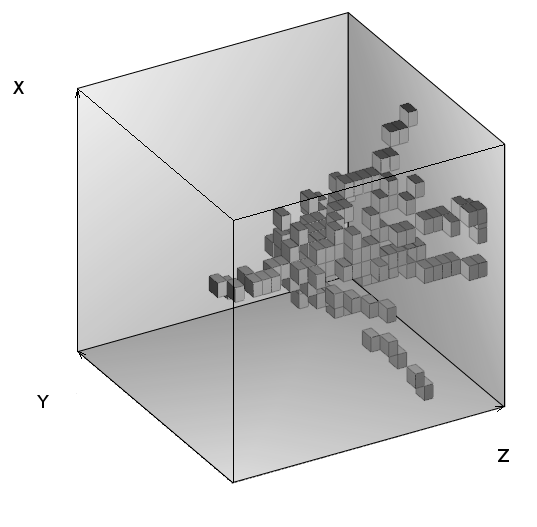
\includegraphics[width=.90\linewidth]{ECAL/graphics/before.png}
		\caption{\label{fig:before} \sl with interaction region.}
	\end{subfigure}% 
	\begin{subfigure}{0.5\textwidth}
		\centering
		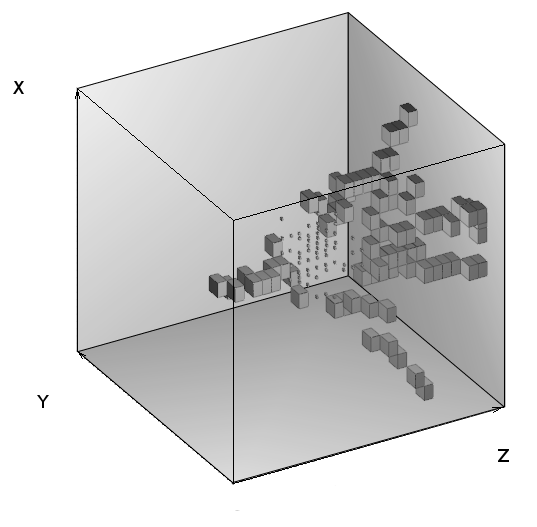
\includegraphics[width=.90\linewidth]{ECAL/graphics/after2.png}
		\caption{\label{fig:after} \sl without interaction region.}
	\end{subfigure}
	\caption{ \sl {\bf Propose to show a real event} Event display of a primary pion with an energy of 10\,GeV simulated using the \ftfp\ physics list before \textit{(a)} and after removal of the interaction region \textit{(b)}. Smaller cubes are pads that are part of the interaction region and are not processed by the \tfa . In this event the hits in the first ten layers are classified as hits left by a primary particle.}
	
	\label{fig:test}
\end{figure}

Figure \ref{fig:before} displays a simulated event after noise and isolated hits filters and Fig. \ref{fig:after} is the same event after removal of the interaction region. As can be seen in Fig. \ref{fig:after} the interaction region is the starting point for secondary tracks.

%The energy deposition in the interaction region of the $\mathrm{\pi}^-$ events in \ecal\ is analyzed in Sec. \ref{sec:results}.

%|||||||||||||||||||||||clusterisation||||||||||||||||||||||||||||

\subsection{Clusterisation}\label{sec:cluster}
During the clusterisation step the energy depositions that are not associated to the interaction region are grouped into clusters by a topological principle. %This step is needed to separate secondary tracks into corresponding groups of hits, or clusters, for further classification. 

\begin{figure}
	\centering
	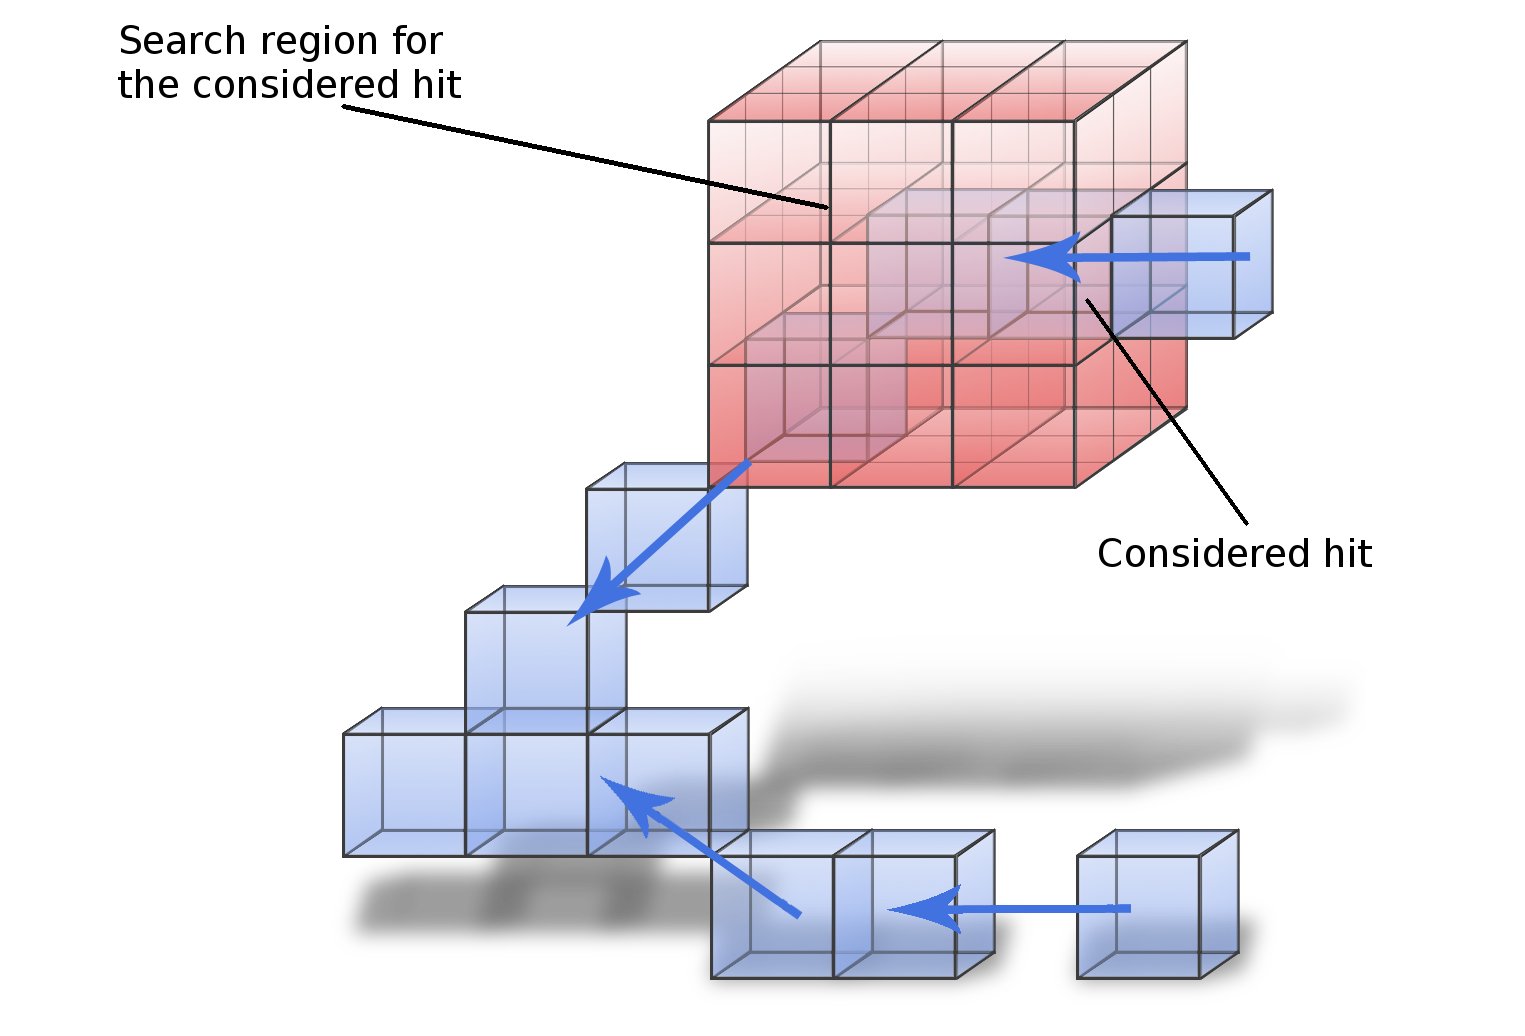
\includegraphics[width=0.5\textwidth]{ECAL/graphics/demo-v2.png}
	\caption{\label{fig:democluster} \sl {\bf Check comment by Eigen on clarity of image} Illustration of the clusterisation step. The \ecal\ hits are represented by blue cubes, and the search region for adjacent hits is indicated by red cubes. The blue arrows point in the direction of the clusterisation flow. }
\end{figure}

%A clusterisation scheme, developed for this study, is called directional recursive clusterisation. 
%The clusterisation algorithm starts recursive assembling of clusters from the last layers of the \ecal, where the secondary tracks are more distinguishable, until the interaction zone or until the first layers in case of MIP-like events. 

The algorithm is described in the following. The description is supported by Fig.\ \ref{fig:democluster}.
%his algorithm has the following steps:
\begin{enumerate}
	\item The separation of tracks improves with increasing distance from the interaction layer. Therefore, hits, isolated within one of the rear layers, seed a cluster. The search for these hits is carried out progressively starting from the last layer in the direction of decreasing $z$.
	Typically, seeding hits are found in the last layer of the detector;
	%For each iteration, the seeding hits for the clusters are taken starting from the last layers of pads to the front layer;
	\item A hit can be associated to a cluster if it was not yet joined to another cluster. This condition excludes the double counting of hits. Effects, arising from ambiguities in the assignment of hits to clusters such as the order in which clusters are created, are expected to be small, but will be addressed in future studies {\bf We haven't addressed this yet!};
	\item For the clusterisation a usual nearest neighbour clustering scheme is applied. More precisely, for each newly associated hit with coordinates $(x_n,y_n,z_n)$ the algorithm finds nearby hits with the following conditions:
	\begin{itemize}
		\item A neighbour hit should have a $z$ coordinate within $[z_n-2,z_n]$
		\item The transverse coordinates of neighbouring hits is searched within ranges $[x_n-1,x_n+1]$ and $[y_n-1,y_n+1]$
	\end{itemize}
	The search region for nearby hits is visualised  in Fig.~\ref{fig:democluster} as a "red cube" with 3 $\times$ 3 $\times$ 3 pads; 
	%with $z$ coordinate equal or less than $z$ coordinate of considered hit
	\item  For each newly associated hit the Steps 2 and 3 are repeated until the process reaches the first layer of the calorimeter or until no more neighbour hits are found.
\end{enumerate}
The choice of this clusterisation method is motivated by a maximum correspondence between the number of clusters and the number of detected tracks.

%|||||||||||||||||||||||Classification||||||||||||||||||||||||||

\subsection{Classification and merging}
\label{sec:class}
Long-lived charged secondary particles from hadronic interactions are expected to leave straight MIP-like tracks in the detector.
The goal of the classification of the clusters obtained in the previous step is thus to select track-like clusters. %and reject clusters left by electromagnetic interaction or detector noise.
%A track-like cluster is defined as a cluster with hits, spatially arranged in the way, that a trajectory of a single charged particle can go through the most of its pads with energy depositions.

The classification algorithm executes the following steps:
\begin{enumerate}
	\item Reject all clusters with 2 hits ($N_{hits}$) as residual noise clusters;
	\item Calculate the length $l$ of the considered cluster as the maximal distance between any pair of hits that are in the cluster;
	\item A cluster is rejected if it has a length of less than $l_{cut} = 2\,{\rm g. u.}$, which corresponds to the minimal length of a track-like cluster with 3 hits; 
	\item Compute  the following observable:
	\begin{equation}
	\label{eq:observable}
	\xi = \frac{l}{N_{hits}-1} + \varepsilon N_{hits},
	\end{equation}
	as a measure for the eccentricity of the cluster. 
	The first term of Eq.~\ref{eq:observable} in motivated by the linear dependence of $N_{hits}-1$ on the cluster length $l$, illustrated in Fig.~\ref{fig:lnhits}.
	The second term introduces a free parameter $\varepsilon$ as an ad hoc correction to increase the efficiency for selecting clusters that do not conform to the nominal pencil-like topology, as explained below.
	The value of the parameter was chosen to be $0.03$ after visual inspection of a few tens of events in the event display;
	%In Eq. \ref{eq:observable} $\varepsilon$ is a free parameter to correct for non-ideal pencil like clusters. 
	%The parameter $\varepsilon$ takes values much smaller than 1. 
	\item If $\xi \geq 1$ a cluster is considered as track-like. Otherwise, the cluster can be classified as e.g. two inseparable tracks.
\end{enumerate}
Due to a number of effects like multiple scattering, residual detector-noise, $\delta$-rays or the residual arbitrariness in the assignment of hits to clusters, the reconstructed tracks are in general not exactly pencil-like.  
The correction term $\varepsilon N_{hits}$ in the definition of $\xi$ serves to keep a cluster as track-like even if it has large $N_{hits}$ and its form is not strictly pencil-shaped, i.e. $l / (N_{hits}-1) < 1$.

A deeper discussion of the effects of the  \ep\ is presented in Sec. \ref{sec:systematics}. 

\begin{figure}
	\centering
	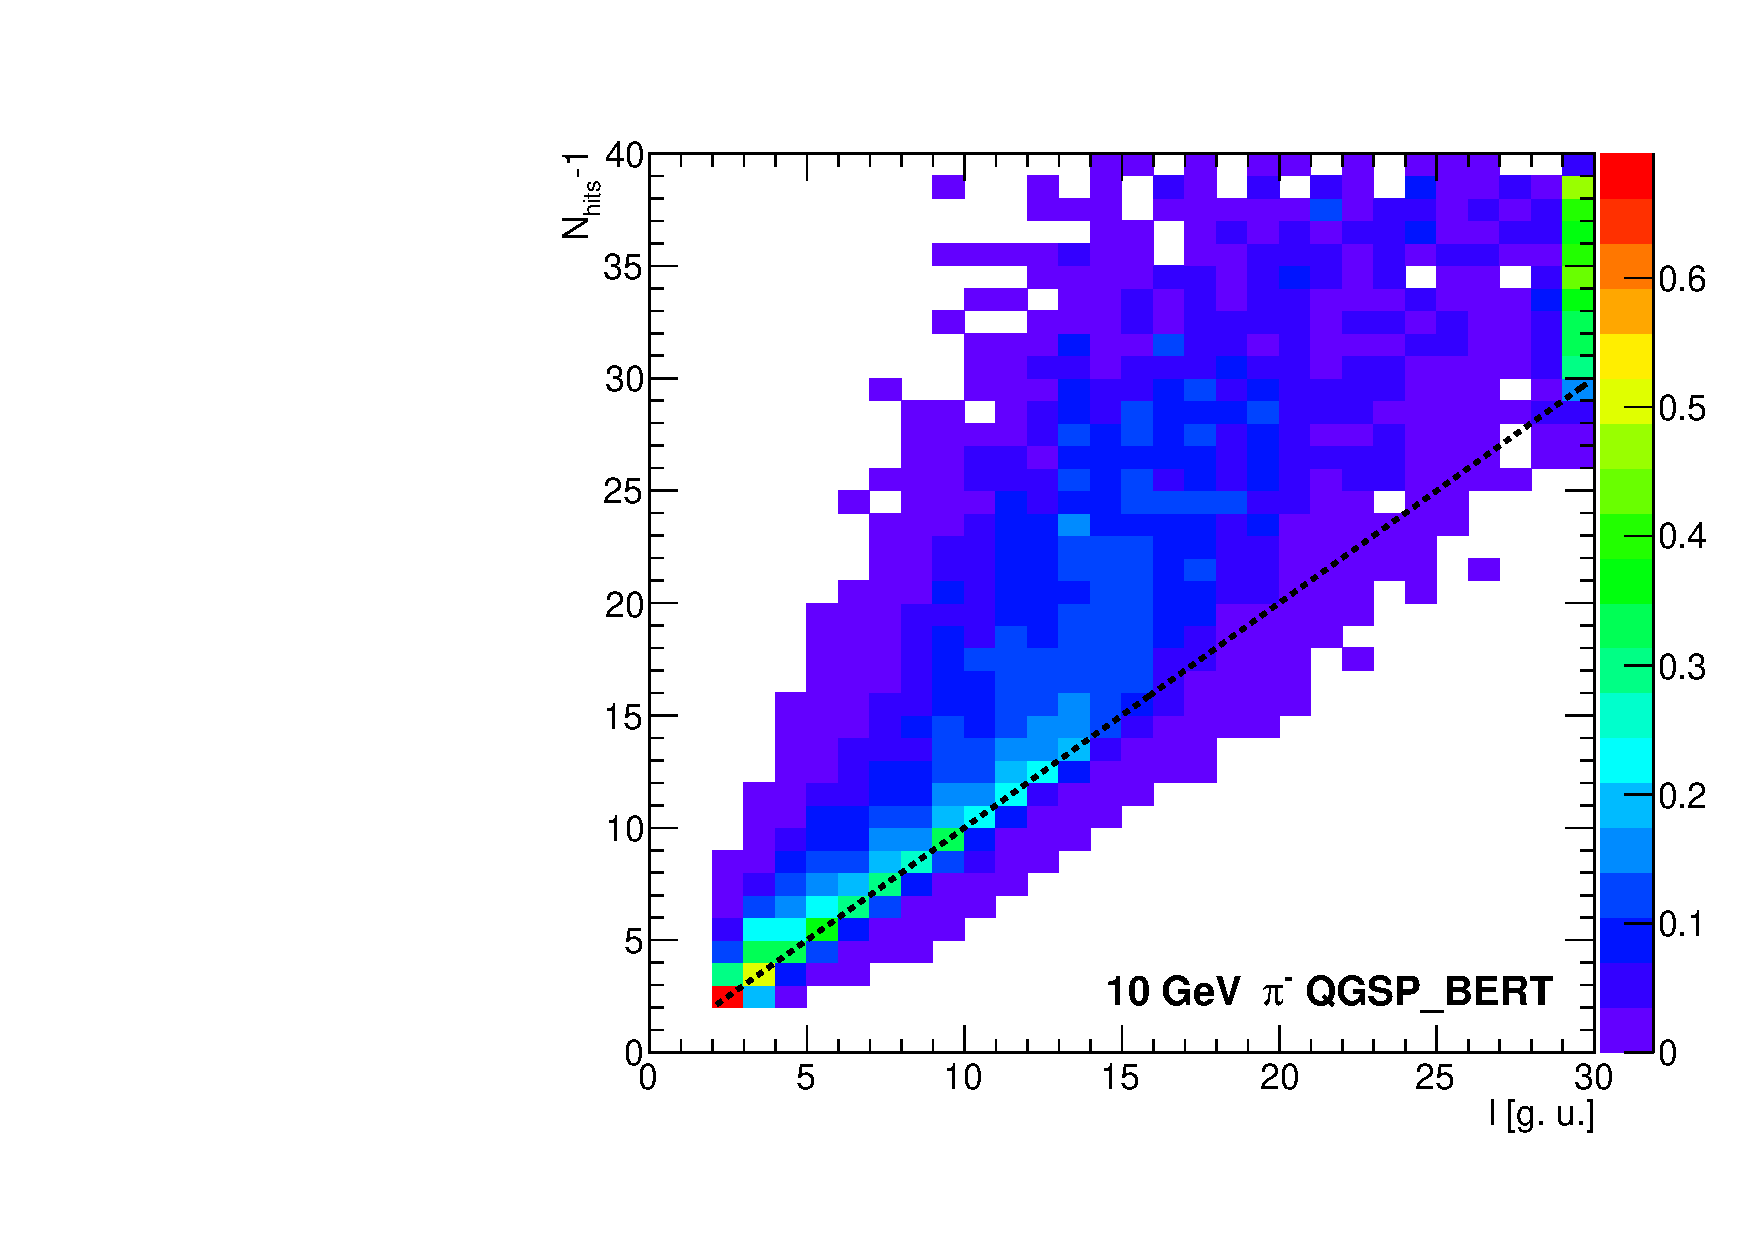
\includegraphics[width=0.5\textwidth]{ECAL/plots/l-nhits.pdf}
	\caption{\label{fig:lnhits} \sl Correlation between $N_{hits} - 1$ and cluster length $l$ in ${\sl g.u.}$ at the example of simulated pions with an energy of 10\,GeV using the \qgsp\ physics list. To guide the eye a line for $N_{hits} - 1=l$ is included in the figure.}
\end{figure}


\begin{figure}
	\centering
	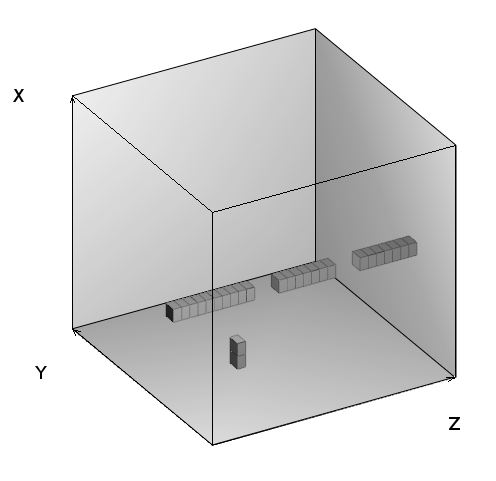
\includegraphics[width=0.5\textwidth]{ECAL/graphics/segmented-track-example.png}
	\caption{\label{fig:demomerge} \sl An example of a segmented track in the \ecal\ from a single 6\,GeV $\mu^-$ in \ftfp\ Monte Carlo simulation.}
\end{figure}
The next step of the classification is to detect a cluster from the primary particle. 
If this cluster exists and meets the conditions for a track-like cluster, it affects the track counting and merging algorithm.
A cluster is classified as being produced by the primary particle if it starts in the first module of the \ecal\ and if it encloses a small angle with respect to the $z$-axis. 
An example of a cluster by a primary particle is visible in Fig. \ref{fig:after}. Clusters assigned to primary particles are discarded in the following analysis. 

Different track-like clusters that correspond to track segments from a single particle, see Fig. \ref{fig:demomerge}, have to be merged into a single track. 
The merging procedure combines track-like clusters with any type of clusters using a simple cone algorithm.
%Because of limitations of clusterisation method, 
%A segmented track from a secondary particle can be divided into two different clusters as it is shown in Fig. \ref{fig:demomerge}.
%It is thus necessary to merge different track segments from a single particle into one track-like cluster. 
%The merging procedure combines track-like clusters with any type of clusters using a simple cone algorithm. 
%TODO: extend merging?
Tested on a sample of single, isolated muons with an energy of 6\,GeV simulated with the \ftfp\ physics list, the \tfa\ finds correctly only one track with 99.7\% efficiency. The sample contains about 3\% events with segmented tracks. 


%------------------------------------------------------------
%----------------------SYSTEMATICS---------------------------
%------------------------------------------------------------

%\subsection{Study of systematics}
\subsection{Discussion of the \ep }
\label{sec:systematics}


The \tfa\ depends on a number of parameters. The biggest sensitivity of the \tfa\ is expected to be introduced by the empirically defined \ep, see Eq.~\ref{eq:observable}. 
Therefore its influence on the results and a further motivation of the choice of the working point in terms of the \ep\, is given in the following. 

After the cut on the minimum cluster length $l_{cut}$, see Sec. \ref{sec:class}, all clusters with 3 hits are track-like, independently of the $\varepsilon$ value.
Therefore, these clusters are not considered in this discussion. 

Figure \ref{fig:epsilonsys} shows the dependence of $\left<N_{tracks}\right>$ on $\varepsilon$ for different beam energies\footnote{\label{note3}The mean number of tracks as function of $\varepsilon$ in data and simulation is given in Appendix~\ref{app:a} for future reference.}.
Each curve has its minimum value at $\varepsilon = 0$ that is the mean number of ideal pencil-like tracks per event and saturates at large $\varepsilon$, when each cluster is taken as track-like.  
%As can be seen from Fig. \ref{sec:systematics} mean number of tracks strongly depend on chosen \ep\ value that needs to be constrained. 
\begin{figure}
	\centering
	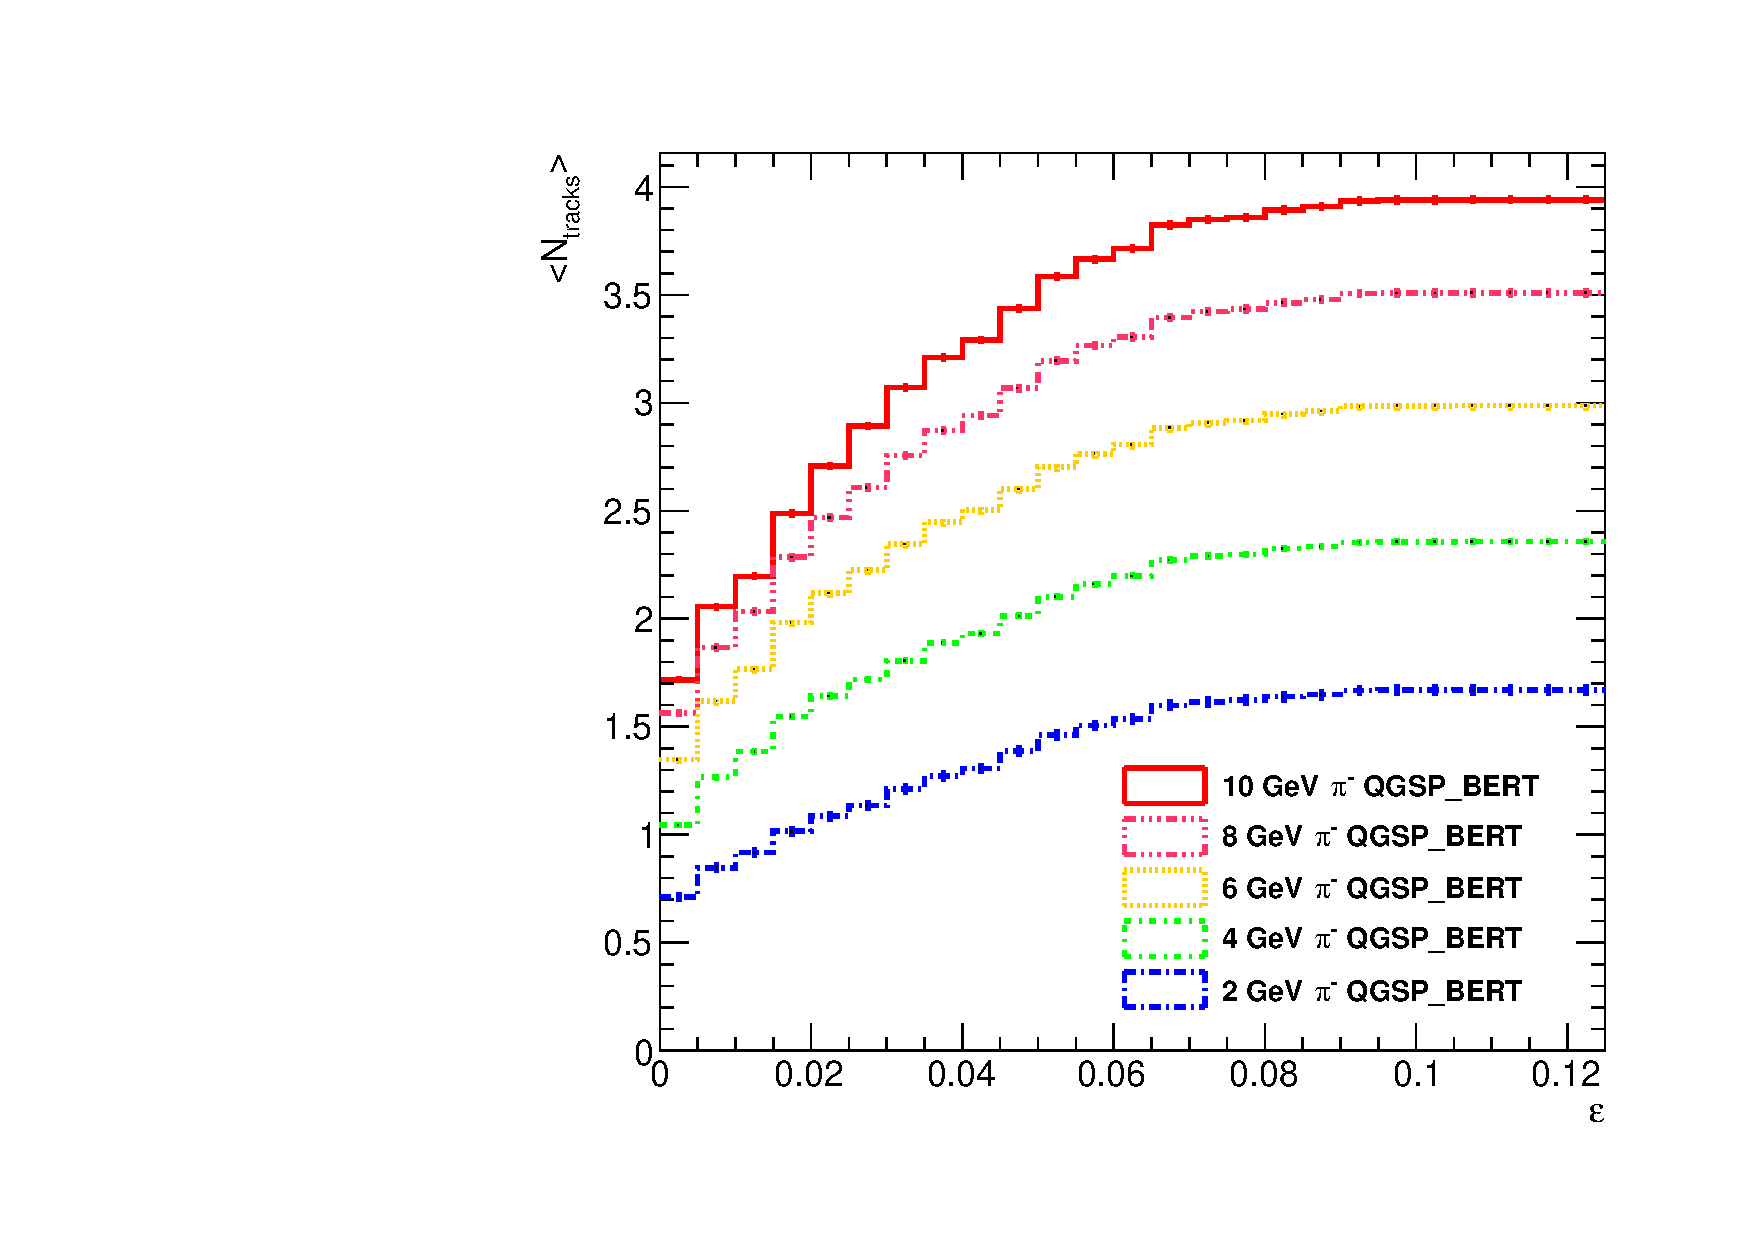
\includegraphics[width=0.5\textwidth]{ECAL/plots/comparison.pdf}
	\caption{\label{fig:epsilonsys} \sl Mean number of tracks found by the \tfa\ as a function of $\varepsilon$ for 2, 4, 6, 8 and 10\,GeV beam energy for the \qgsp\ physics list simulation. Events without a detected interaction region are discarded.}
\end{figure}

For all clusters with a number of hits larger than 3, the simulated muon and electron samples are used to define a motivated choice for the value of  $\varepsilon$ to be applied for the track finding. 

A Monte Carlo sample of $\mu^-$ is used to determine a lower bound on the \ep. The events for this study are selected if the number of hits is larger than the number of layers in the \ecalp. After this cut the muon tracks do not have a straight pencil-like shape, but rather a line with a number of adjacent hits generated by residual detector noise or $\delta$-rays. An example of such a track is given in Fig. \ref{fig:muonsys}.
\begin{figure}
	\centering
	\begin{subfigure}{0.5\textwidth}
		\centering
		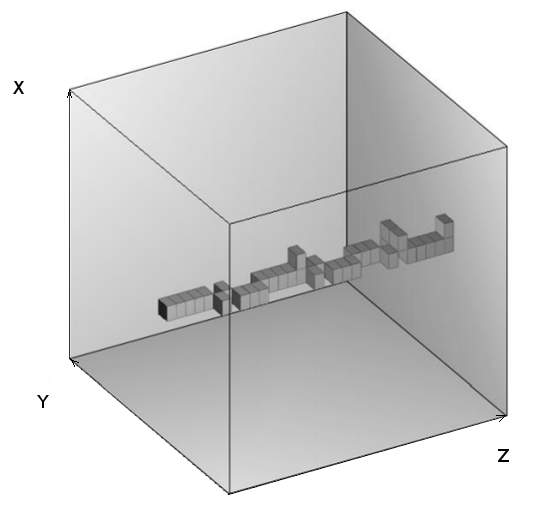
\includegraphics[width=.90\linewidth]{ECAL/graphics/muon-sys.png}
		\caption{\label{fig:muonsys}}
	\end{subfigure}% 
	\begin{subfigure}{0.5\textwidth}
		\centering
		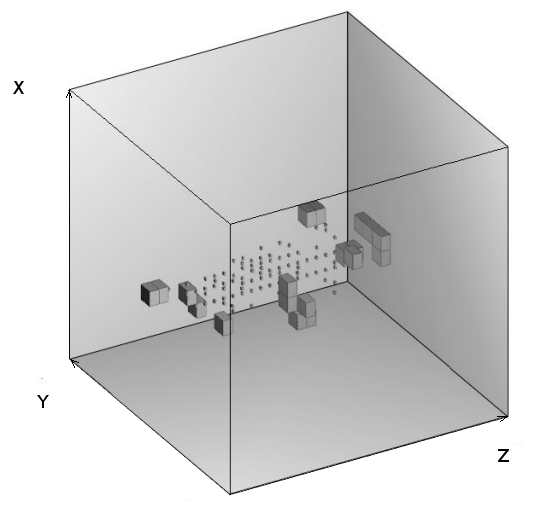
\includegraphics[width=.90\linewidth]{ECAL/graphics/e-sys.png}
		\caption{\label{fig:esys}}
	\end{subfigure}
	\caption{ \sl Event displays of simulated events showing a muon with an energy of 10 GeV after selection by the number of hits in \ecal\ \textit{(a)} and a 6\,GeV electron after removal of the interaction region \textit{(b)}.}
\end{figure}
The resulting sample represents secondary tracks from hadronic interactions with noise or other additional hits from the debris of the interaction region. 

%The electron Monte Carlo sample after the interaction region filter is used to establish an upper bound on the \ep\ value. 
A Monte Carlo sample based on electrons is used to estimate an upper bound on $\varepsilon$. Electrons are not expected to generate tracks but rather only an interaction region accompanied  by low energetic satellite clusters, see Fig~\ref{fig:esys}. Events in this sample contain only non track-like clusters. 
\begin{figure}[H]
	\centering
	\begin{subfigure}{0.5\textwidth}
		\centering
		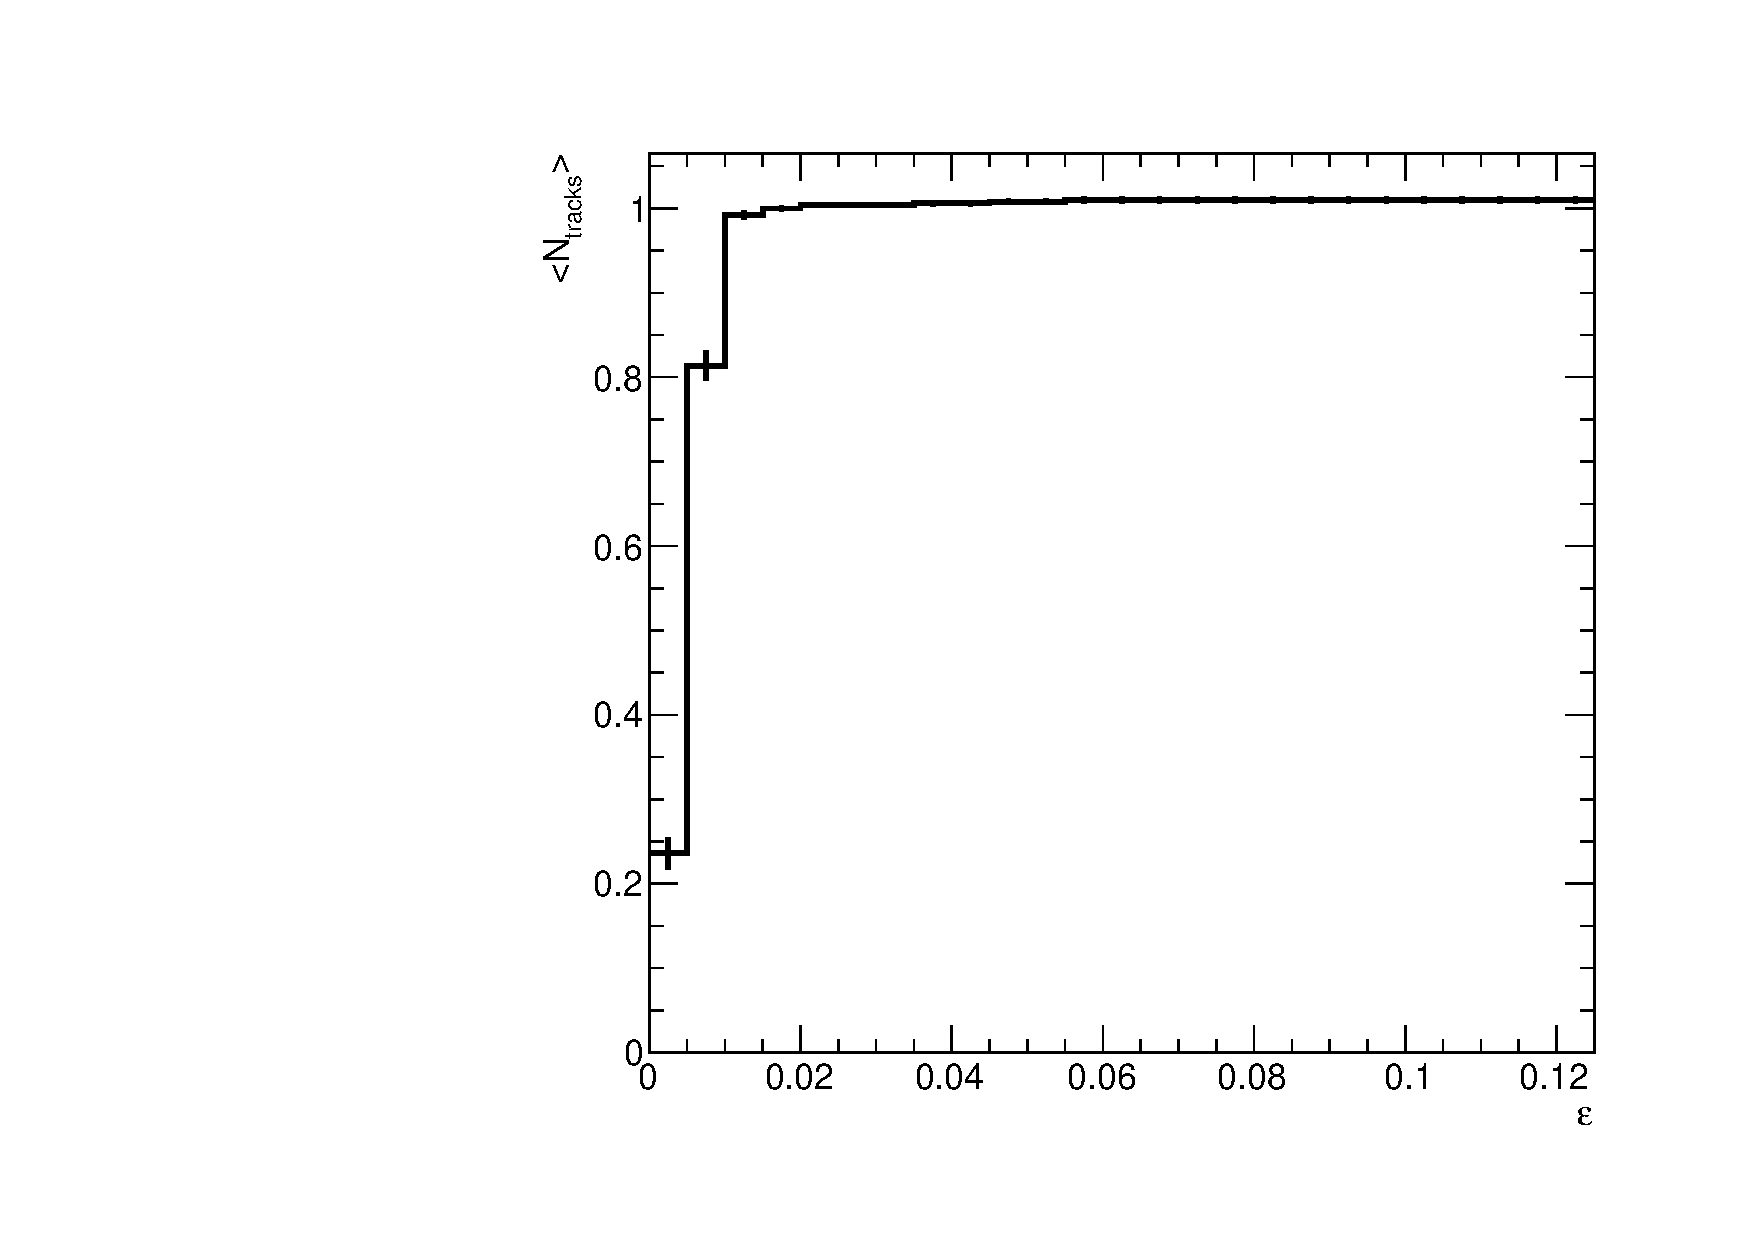
\includegraphics[width=.90\linewidth]{ECAL/plots/muon-sys.pdf}
		\caption{\label{fig:muonhistsys} \sl muon sample}
	\end{subfigure}% 
	\begin{subfigure}{0.5\textwidth}
		\centering
		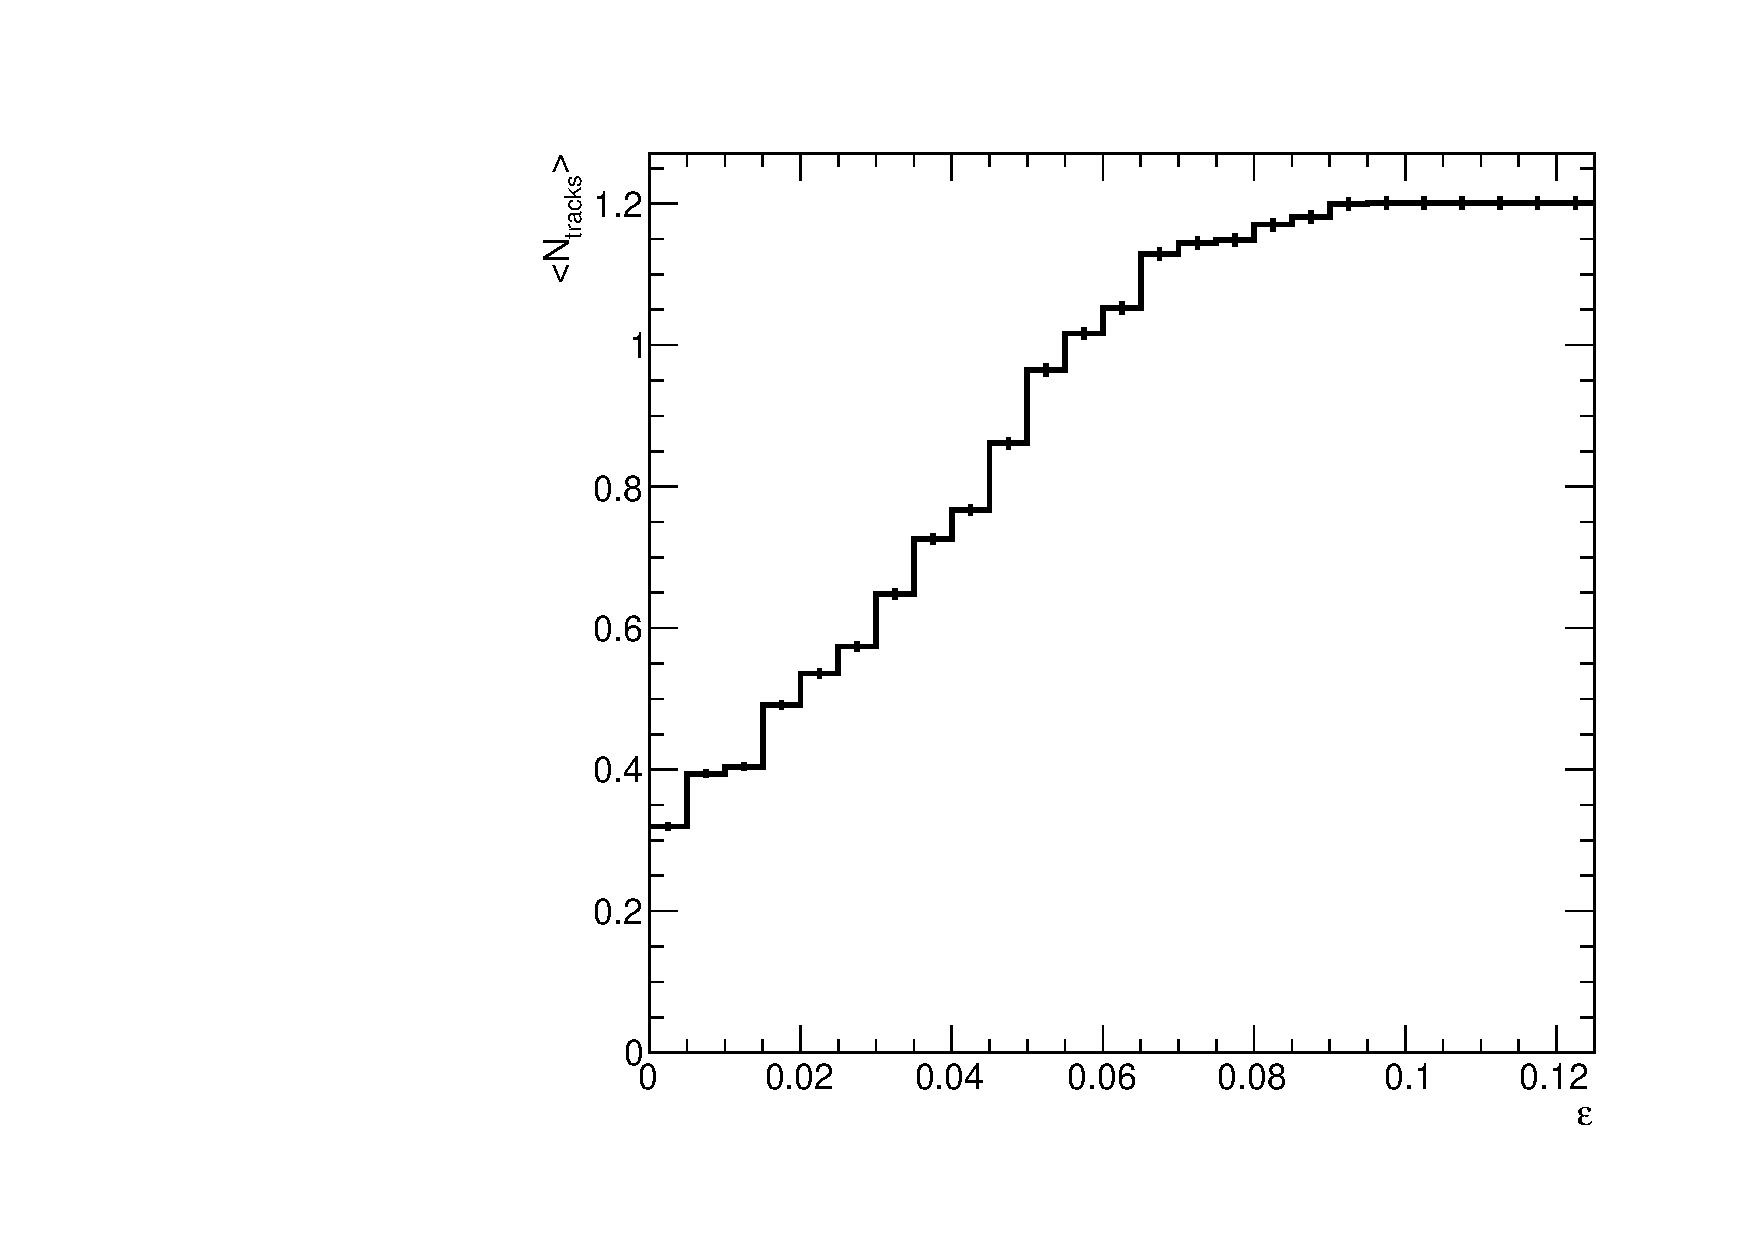
\includegraphics[width=.90\linewidth]{ECAL/plots/electron-sys.pdf}
		\caption{\label{fig:ehistsys} \sl electron sample}
	\end{subfigure}
	\caption{\label{fig:muehistsys} \sl The distribution of $\left<N_{tracks}\right>$ in simulated events as a function of $\varepsilon$ for  \textit{(a)} 10\,GeV $\mathrm{\mu}^-$ after selection by the number of hits in \ecal\ and \textit{(b)} 6\,GeV electrons after removal of the interaction region .}
\end{figure}

Figure \ref{fig:muehistsys} shows the dependence of $\left<N_{track}\right>$ on $\varepsilon$ for the muon (Fig. \ref{fig:muonhistsys}) and electron (Fig. \ref{fig:ehistsys}) samples. 
%The lower bound $\varepsilon_{low}$ on \ep\ value is set to give $N_{tracks} = 1$ on average in muon sample, and upper bound $\varepsilon_{up}$ is defined as $N_{tracks} = 1$ on average in electron sample.
The lower bound $\varepsilon_{low}$ of the \ep\ is identified with the value of $\varepsilon$ for which $\left<N_{tracks}\right> \simeq 1$ in the muon sample. Correspondingly, the upper bound $\varepsilon_{up}$ is identified with that value of $\varepsilon$ for which $\left<N_{tracks}\right> = 1$ in the electron sample.
The approximate values are:
\begin{equation}
\varepsilon_{low} \simeq 0.015\ \texttt{and}\ \varepsilon_{up} \simeq 0.05.
\end{equation}
The empirically chosen value for $\varepsilon$ of $\varepsilon = 0.03$ lies within these bounds. 

As the algorithm is a new development it will be convenient to give the reader a feeling on the sensitivity of the results with respect to the actual choice of the \ep\,
For this the estimator 
\begin{equation}
S_{{\cal O}} = \frac {\left<{\cal O}(\varepsilon_{1}) - {\cal O}(\varepsilon_{2})\right>}  {\left<{\cal O}(\varepsilon_{nom})\right>}
\label{eq:sens}
\end{equation}
is introduced and will be evaluated in Sec.~\ref{sec:results} where applicable.

Further dependencies of the \tfa\ on the value of the cone angle of the merging algorithm, initial MIP exclusion and residual noise are expected to be small but will be addressed for the final paper.
%Other systematic effects coming from value of the cone angle of the  merging algorithm and initial MIP exclusion are expected to be small. %(TODO)

%------------------------------------------------------------------
%---------------------------RESULTS--------------------------------
%------------------------------------------------------------------

\section{Results}
%Systematic uncertainties related to the calorimeter calibration, event selection and preprocessing are discussed in Ref. \cite{bib:Naomi}.
\label{sec:results}
%\subsection{Comparing Monte Carlo models with data}
%Various Monte Carlo models are compared with the test beam data in terms of the interaction region parameters, and secondary tracks observables. The following figures show these comparisons for simulations based on the two studied Monte Carlo physics lists.
In the following observables on the interaction region and on secondary particles as obtained in beam test data are compared with simulations based on the three {\sc Geant4} physics lists introduced above. According to~\cite{Bilki:2014uep} the data are contaminated after the pre-selection with 8.8\% double-$\pi$ events at 2\,GeV and as low as 1.5\% at 10\,GeV. The Monte Carlo samples have thus been produced with an admixture of double-$\pi$ events for the comparison with the data. When averaged results are shown, correction factors will be extracted by comparing the results for contaminated samples with those from pure samples.  The correction factors will be given by the means calculated from the individual correction factors extracted from the two physics lists. The uncertainty on the correction factors will constitute the systematic error and is given by the difference between the mean corrections factor and the individual correction factors. The correction factors are between 0.93 and 1 and the uncertainties are of the order of a few \%. Another source of systematic uncertainty suggested in~\cite{Adloff:2013vra} that may be caused by the uncertainty on the MIP energy scale has been studied and was found to be negligible for the results presented in the following.
%Systematic uncertainties related to the calibration, event selection and preprocessing are discussed in Ref. \cite{bib:Naomi}. 
\subsection{Energy fraction of the interaction region}
%---------------interaction zone--------------------
An intuitive estimator to characterise the interaction of the $\pi^-$  with the absorber material is the fraction $f_{IR}$ of energy deposited in the interaction region $E_{IR}$ over the total energy deposited in the calorimeter $E_{tot.}$. Hence, $f_{IR}$  is defined as
\begin{equation}
f_{IR} = \frac{E_{IR}}{E_{tot.}}
\end{equation}

%In this study the interaction region created by $\pi^-$ interacting with the absorber material is characterised by the fraction $f_{IR}$ of total energy deposited in the calorimeter.% and its lateral radius $r_{IR}$ averaged over hits.

Figure \ref{fig:irexample} shows comparisons of $f_{IR}$ distributions between data and the three {\sc Geant4} physics lists.
The first bin of these histograms corresponds to the fraction of events for which no interaction region is found by the algorithm.
%As can be seen from Fig. \ref{fig:irexample} the fraction of events in this bin for the chosen physics list is approximately(?) compatible with data. 
The rest of the distribution can be briefly described by a skewed normal distribution. The mean value of $f_{IR}$ is shifted towards larger values in data compared with the Monte Carlo simulation. Qualitatively, this observation may suggest for example a different repartition between visible and invisible energy in data and Monte Carlo.

In Fig. \ref{fig:irgraph} the mean value of $f_{IR}$ is shown as a function of the beam energy  for beam energies of 2, 4, 6, 8 and 10\,GeV. Events without a detected interaction region according to Sec.~\ref{sec:iazone} are discarded. An increase of $f_{IR}$ with increasing beam energy from 43\% at 2\,GeV to around 64\% around is observed. Qualitatively this is expected as the electromagnetic component of the hadronic shower becomes increasingly dominant with increasing energy of the primary particle.
In case of the \qgsp\ and \qbbc\  physics list the mean value is up to 20\% smaller than observed in the data.  The \ftfp\ physics list changes its behaviour above 4\,GeV, i.e. at the sharp transition between the Bertini cascade and the Fritiof model bringing the prediction closer to the data.  
The observed discrepancy between data and the predictions by the {\sc Geant4} physics lists is consistent with an underestimation of the total energy deposition by the Monte Carlo models as reported in~\cite{Bilki:2014uep}.


\begin{figure}
	\centering
	\begin{subfigure}{0.5\textwidth}
		\centering
		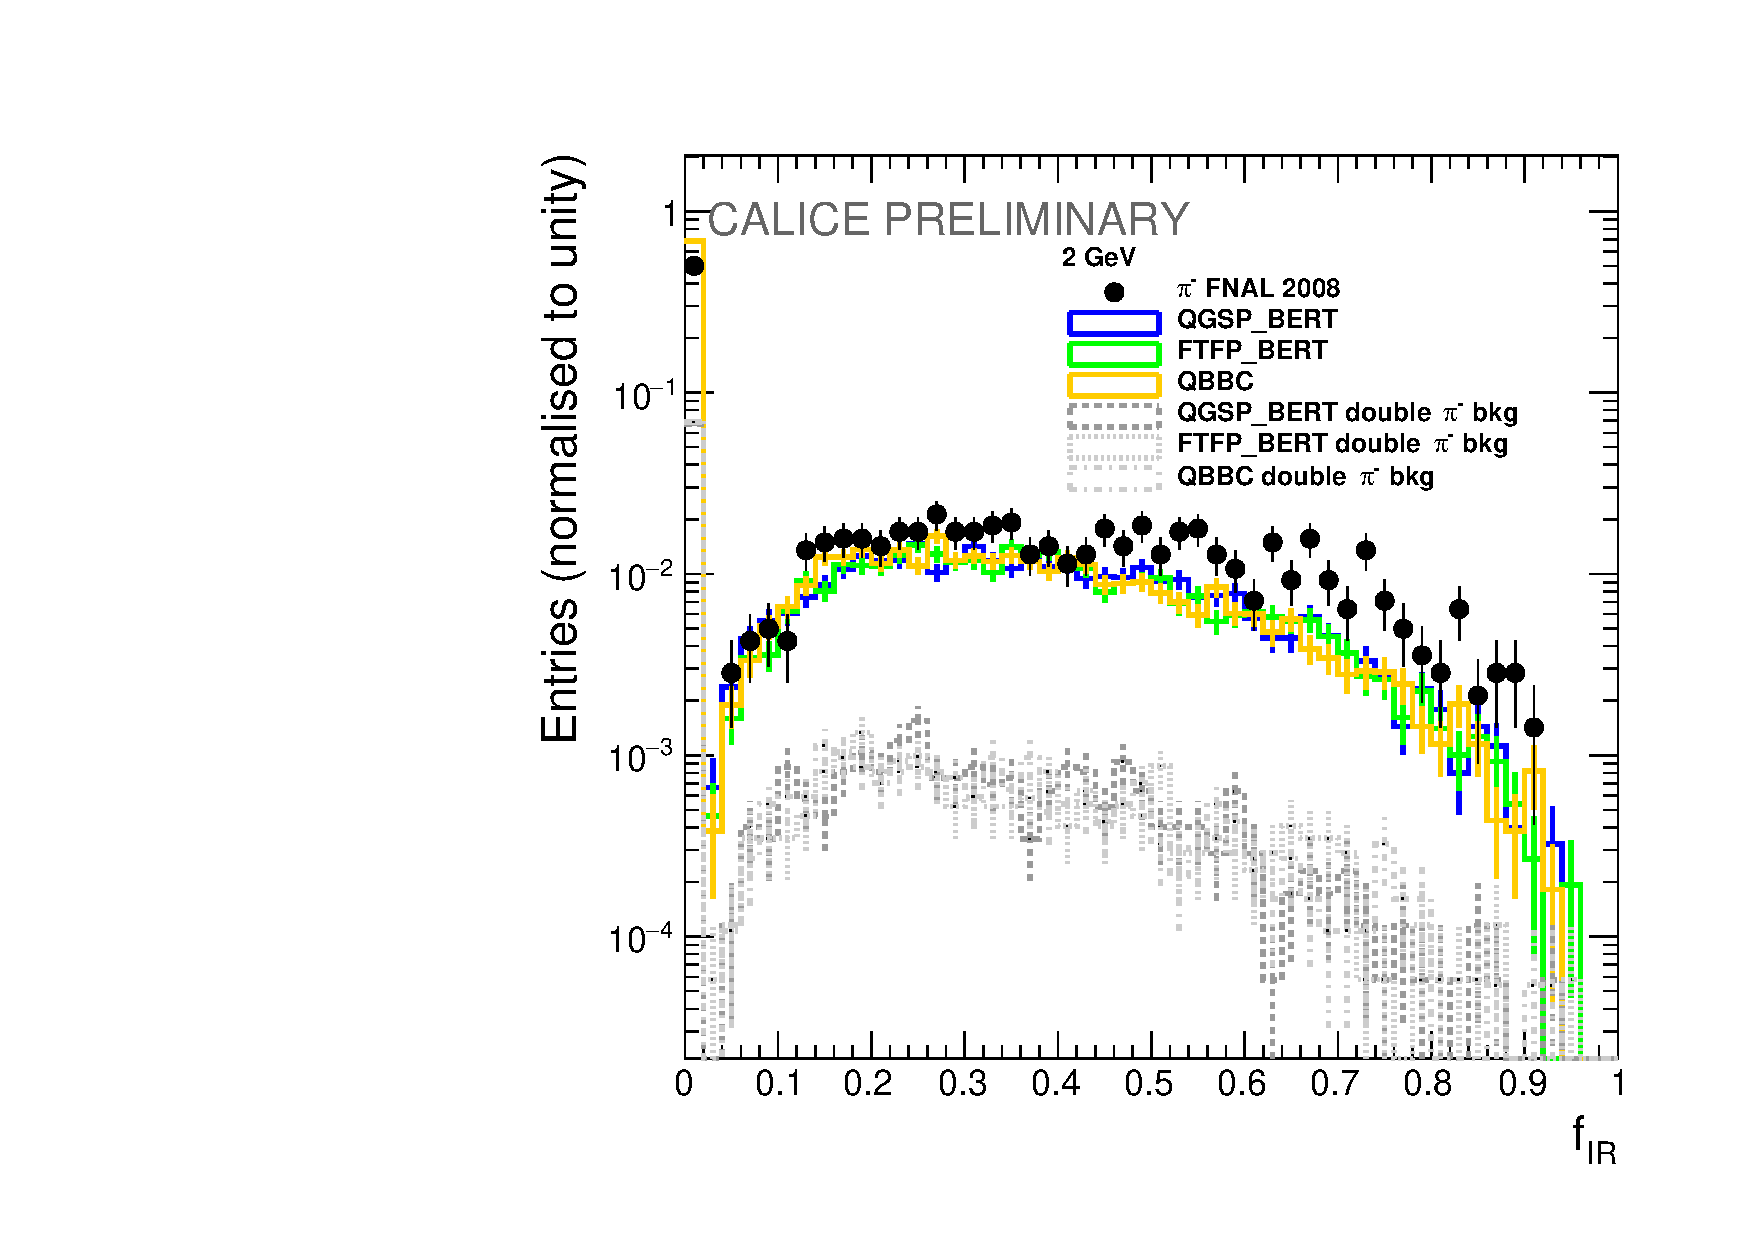
\includegraphics[width=.90\linewidth]{ECAL/plots/e-ir-2.pdf}
		\caption{\label{fig:efr2} }
	\end{subfigure}% 
	\begin{subfigure}{0.5\textwidth}
		\centering
		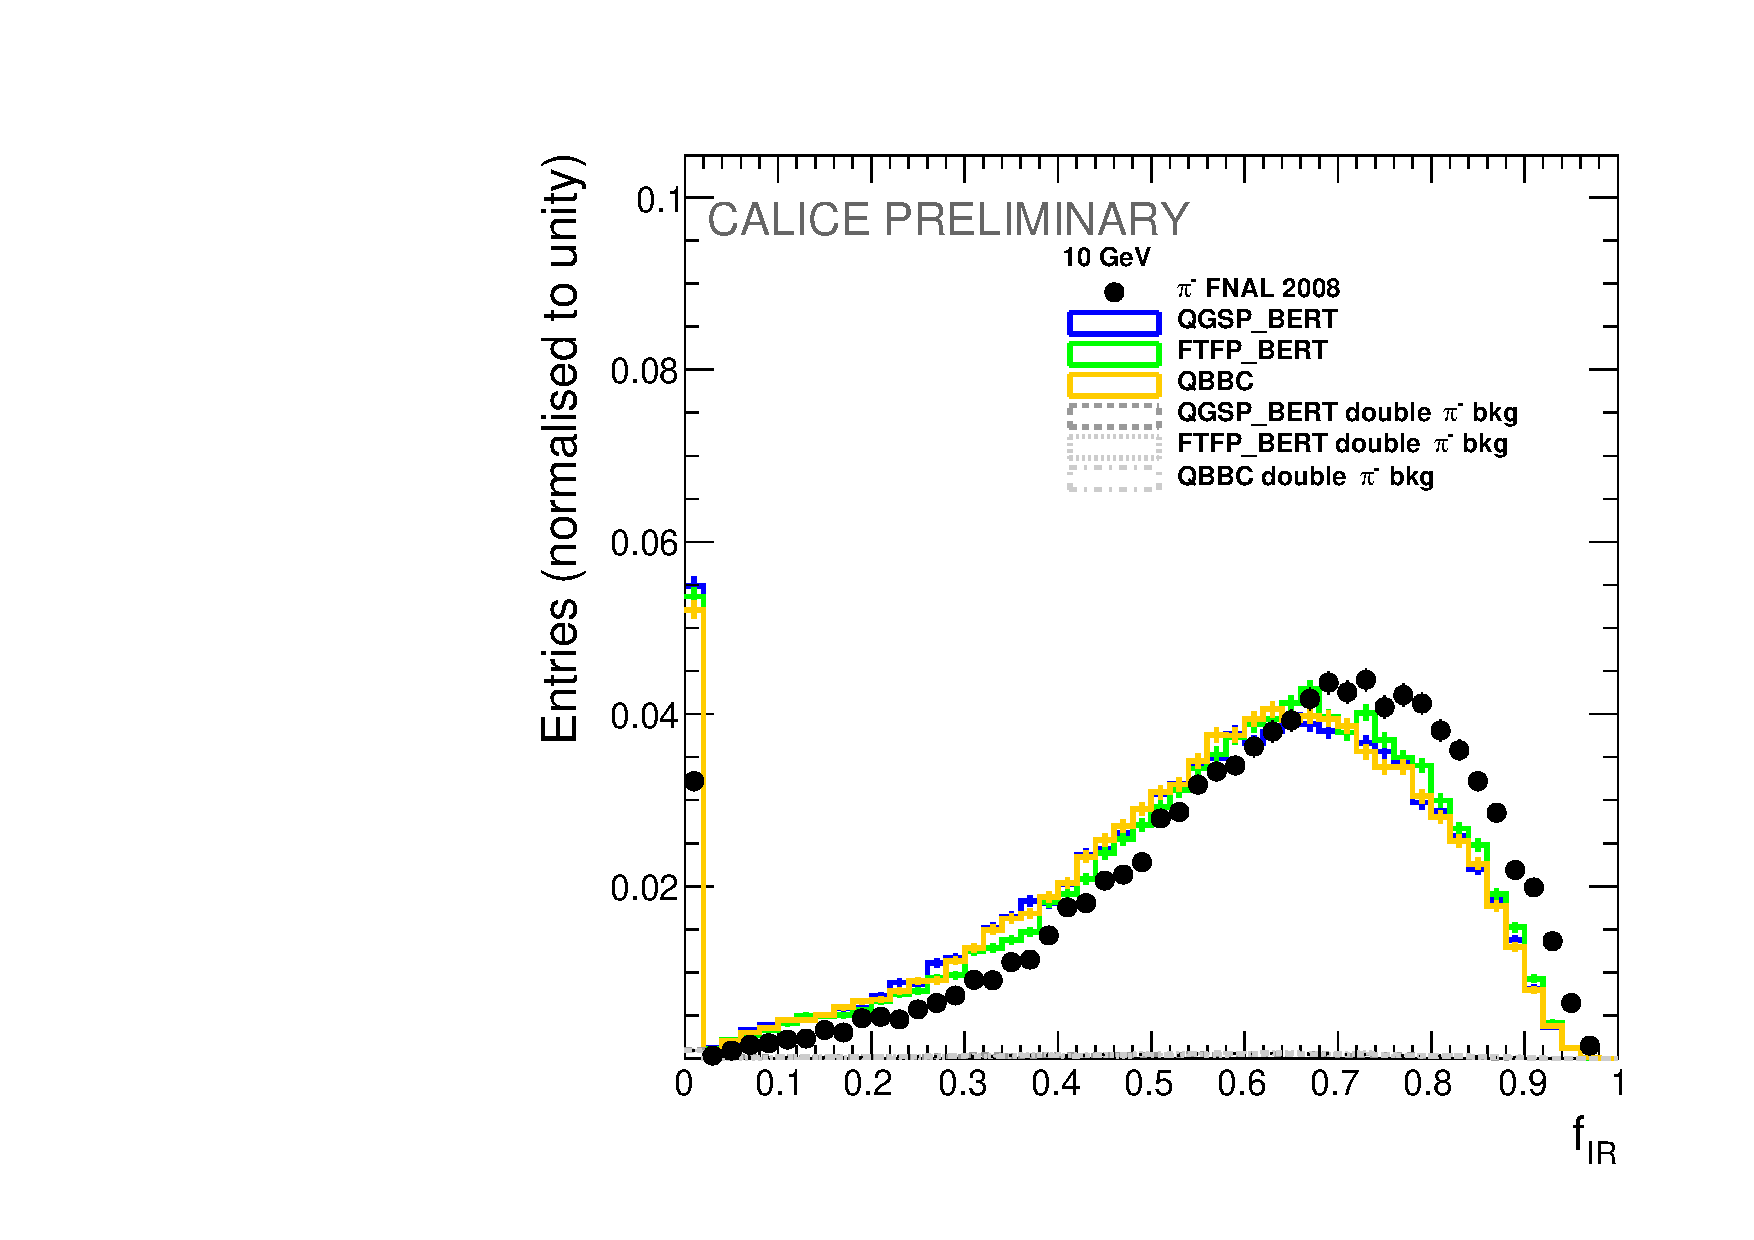
\includegraphics[width=.90\linewidth]{ECAL/plots/e-ir-10.pdf}
		\caption{\label{fig:efr10} }
	\end{subfigure}
	\caption{\label{fig:irexample} \sl {\bf Fig.~\ref{fig:efr2}: Remind me how the linear plot looks like} Comparison of $f_{IR}$ between data and Monte Carlo simulations for two {\sc Geant}4 physics lists for energies of 2 (a) and 10 (b) GeV of the primary particle, respectively. The first bin contains events without a detected interaction region. All histograms are normalised to unity. Error bars represent statistical uncertainties only.}
\end{figure}

\begin{figure}
	\centering
	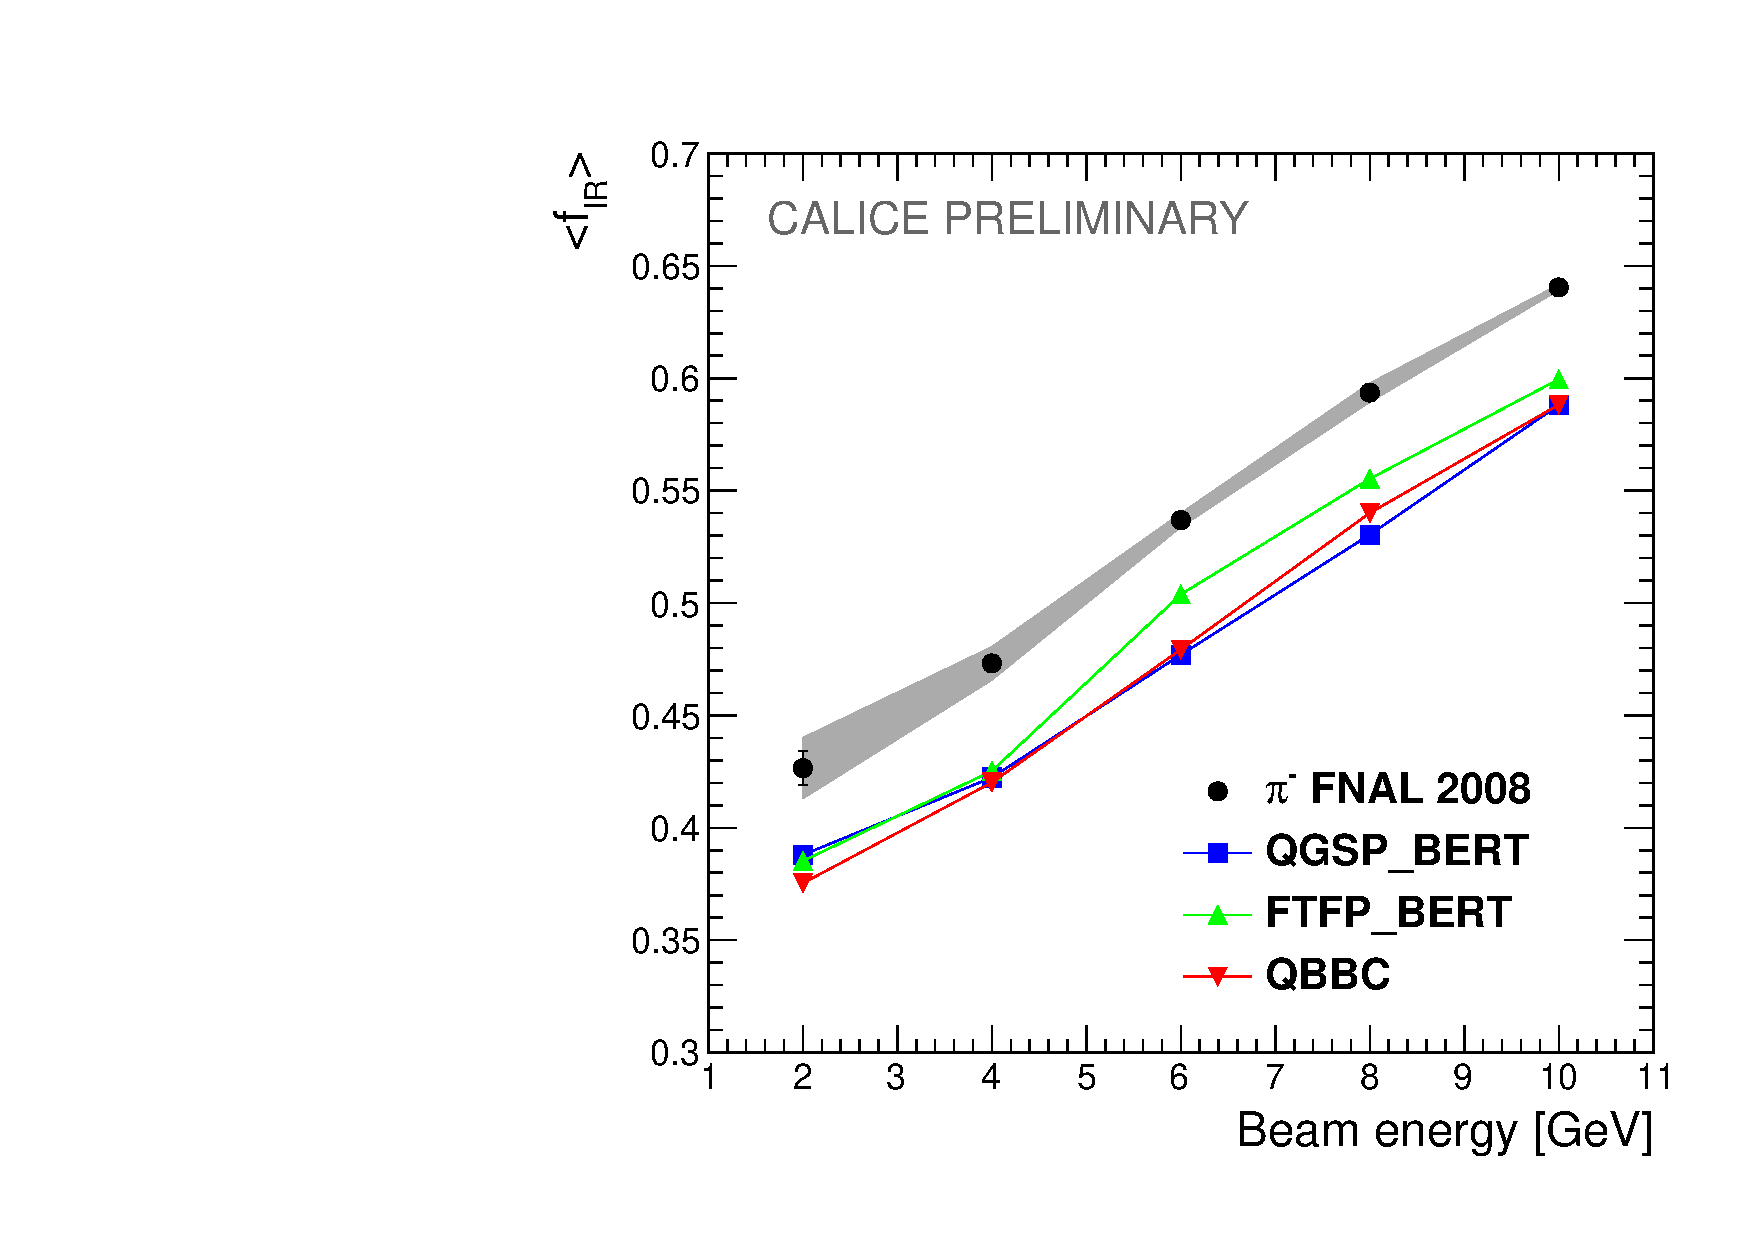
\includegraphics[width=0.5\textwidth]{ECAL/plots/e-ir-graph.pdf}
	\caption{\label{fig:irgraph} \sl  Mean fraction of energy deposition in the interaction region in \ecal\ for data and  Monte Carlo simulations for two {\sc Geant}4 physics lists as a function of the beam energy (2\,GeV to 10\,GeV). Events without a detected interaction region according to Sec.~\ref{sec:iazone} are discarded. The error bars represent statistical uncertainties and the error band the systematic error from the correction for double $\pi$ events.}
\end{figure}
\subsection{Lateral radius of interaction region}
%|||||||||||||||Radius of interaction zone|||||||||||||||||||
%Along with $f_{IR}$, 
The lateral radius $r_{IR}$  of the detected interaction region averaged over hits with respect to the lateral barycentre is a measure of the spatial extension of the interaction region. 
It is defined as:
\begin{equation}
r_{IR} = \frac{\displaystyle \sum_{hit \in IR} \sqrt{(\bar{x}_{IR} - x_{hit})^2 + (\bar{y}_{IR} - y_{hit})^2}} {\displaystyle N_{hits}^{IR}},
\label{eq:rir}
\end{equation}
where the sum runs over the hits in the interaction region, here labeled by $IR$, and $N_{hits}^{IR}$ is the number of hits in the interaction region. In Eq.~\ref{eq:rir} $\bar{x}_{IR}$ and $\bar{y}_{IR}$ are the transversal coordinates of the barycentre of the interaction region that in analogy with Eq.~\ref{eq:barycentre} are defined as: 
\begin{eqnarray}
\label{eq:barycentre2}
\bar{x}_{IR} = \frac{\displaystyle \sum_{hit \in IR} x_{hit}\,E_{hit}}{\displaystyle \sum_{hit \in IR} E_{hit}} 
\text{ and }
\bar{y}_{IR} = \frac{\displaystyle \sum_{hit \in IR} y_{hit}\,E_{hit}}{\displaystyle \sum_{hit \in IR} E_{hit}},
\end{eqnarray}

Distributions of $r_{IR}$ for data and the predictions by the three tested {\sc Geant4} physics lists are displayed in Fig. \ref{fig:rirexample}
for energies of the primary particle of 2\,GeV and 10\,GeV. In both cases the measured interaction region is wider than the predictions by the {\sc Geant}4 physics lists.  
Figure \ref{fig:irrgraph} displays the dependence of the mean $r_{IR}$, $\left<r_{IR}\right>$, on the beam energy for the data and the three {\sc Geant4} physics lists. Here again, events without a detected interaction region according to Sec.~\ref{sec:iazone} are discarded. The lateral size of the interaction region increases with increasing energy of the primary particle. For all tested energies the interaction region measured in data is constantly around 10\% wider than is the case of the {\sc Geant}4 physics lists that lead to identical results. 
%An interpretation of this observation may be that the simulation is lacking energy depositions by secondaries with a comparatively long mean free path length. 

\begin{figure}
	\centering
	\begin{subfigure}{0.5\textwidth}
		\centering
		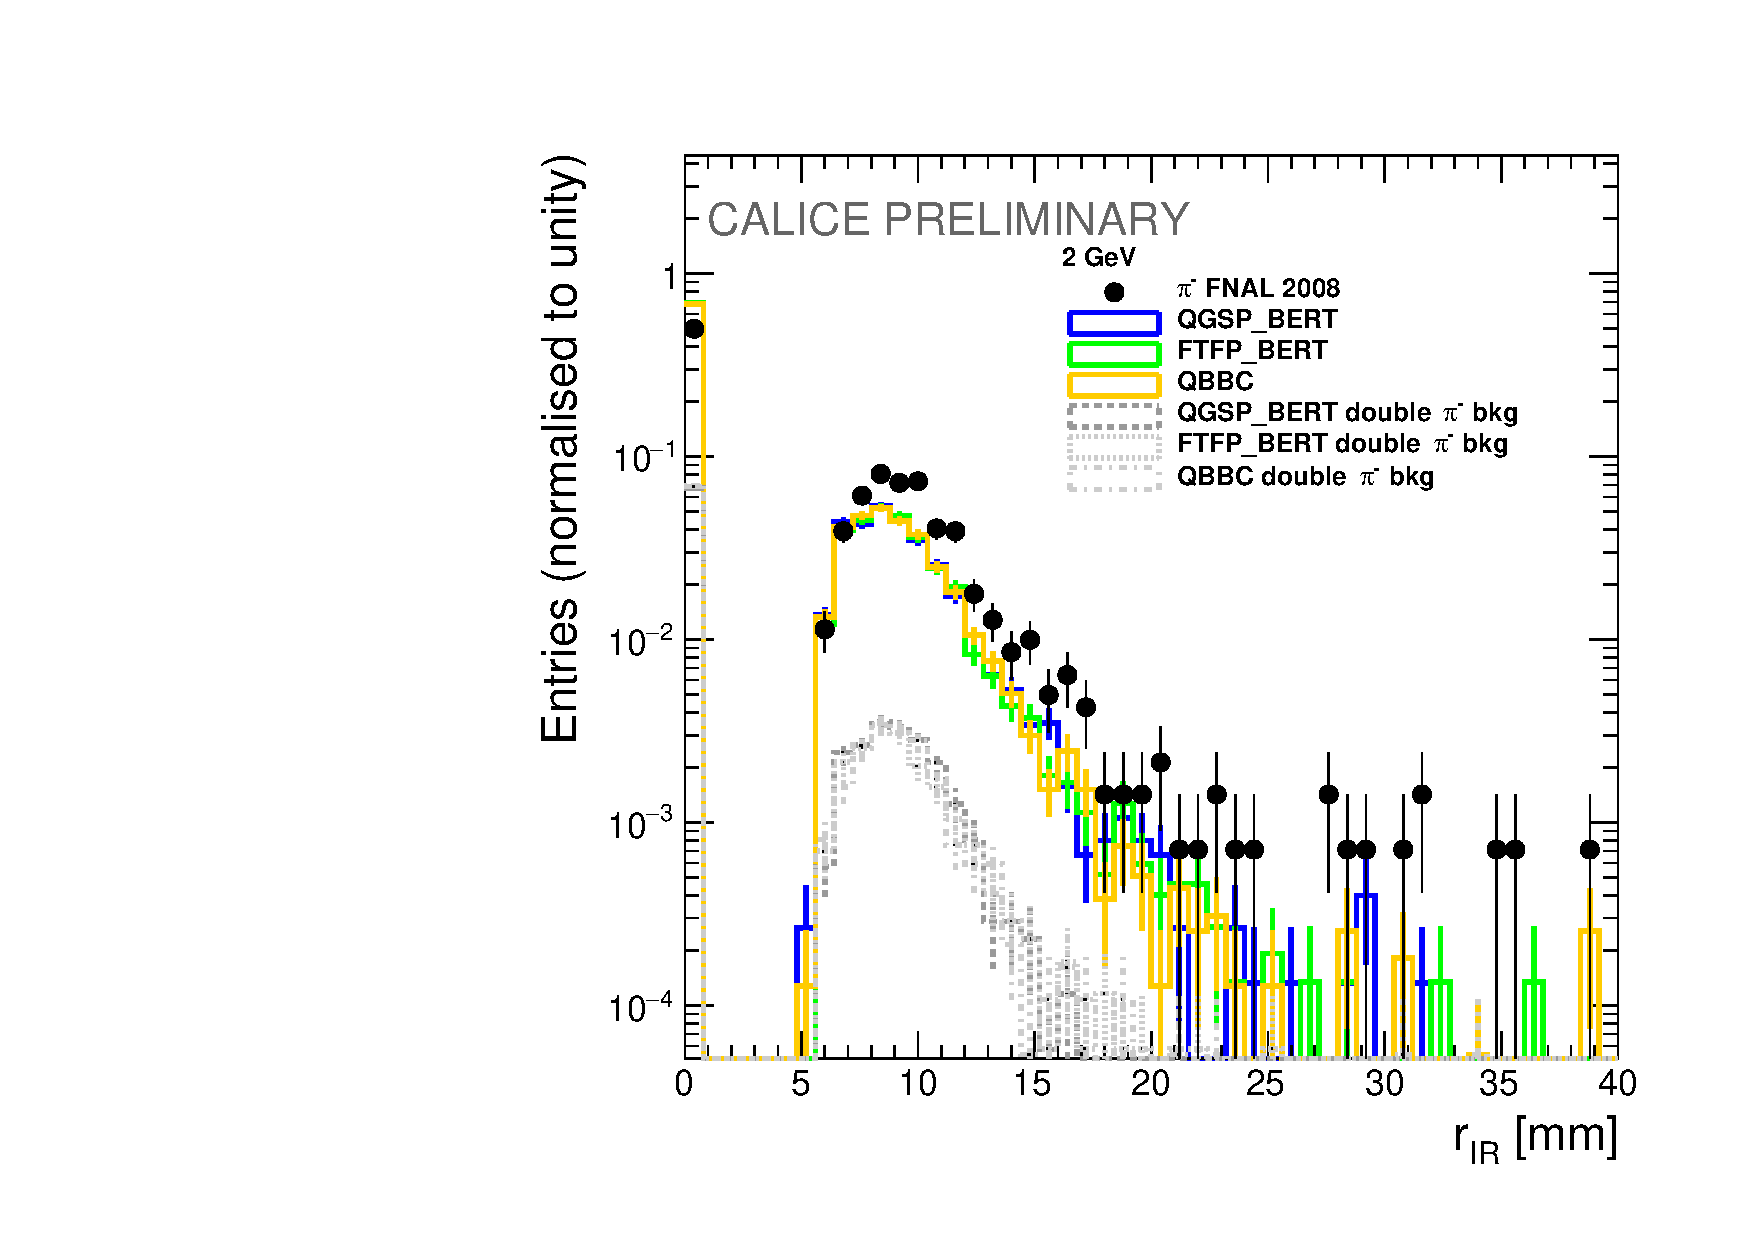
\includegraphics[width=.90\linewidth]{ECAL/plots/r-ir-2.pdf}
		\caption{\label{fig:rir2} }
	\end{subfigure}% 
	\begin{subfigure}{0.5\textwidth}
		\centering
		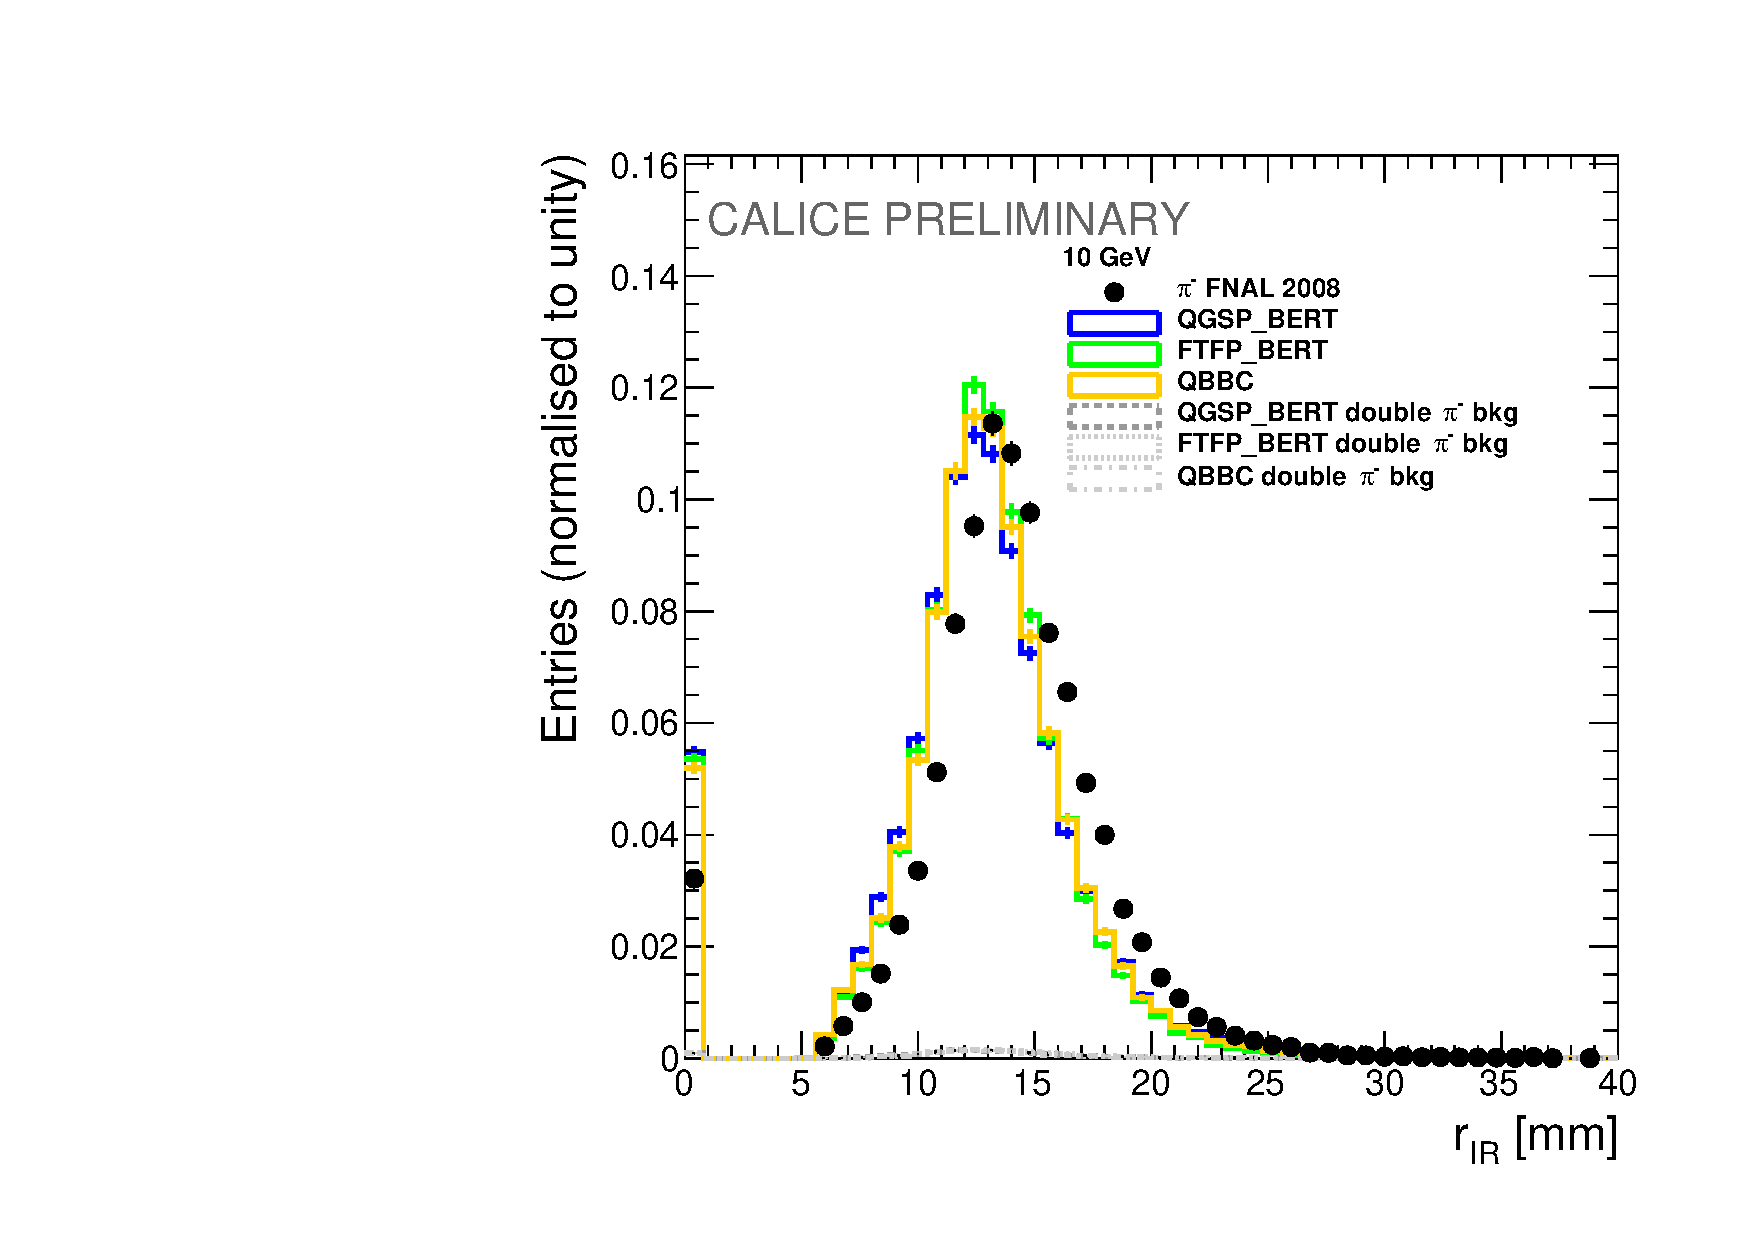
\includegraphics[width=.90\linewidth]{ECAL/plots/r-ir-10.pdf}
		\caption{\label{fig:rir10} }
	\end{subfigure}
	\caption{\label{fig:rirexample} \sl {\bf Same remark as for Fig.~\ref{fig:efr2} } Comparison of $r_{IR}$ distributions for data and Monte Carlo simulations for two {\sc Geant}4 physics lists for energies of the primary particle of 2 (a) and 10 (b) GeV, respectively. All histograms are normalised to unity. Error bars represent statistical uncertainties only.}
\end{figure}

\begin{figure}
	\centering
	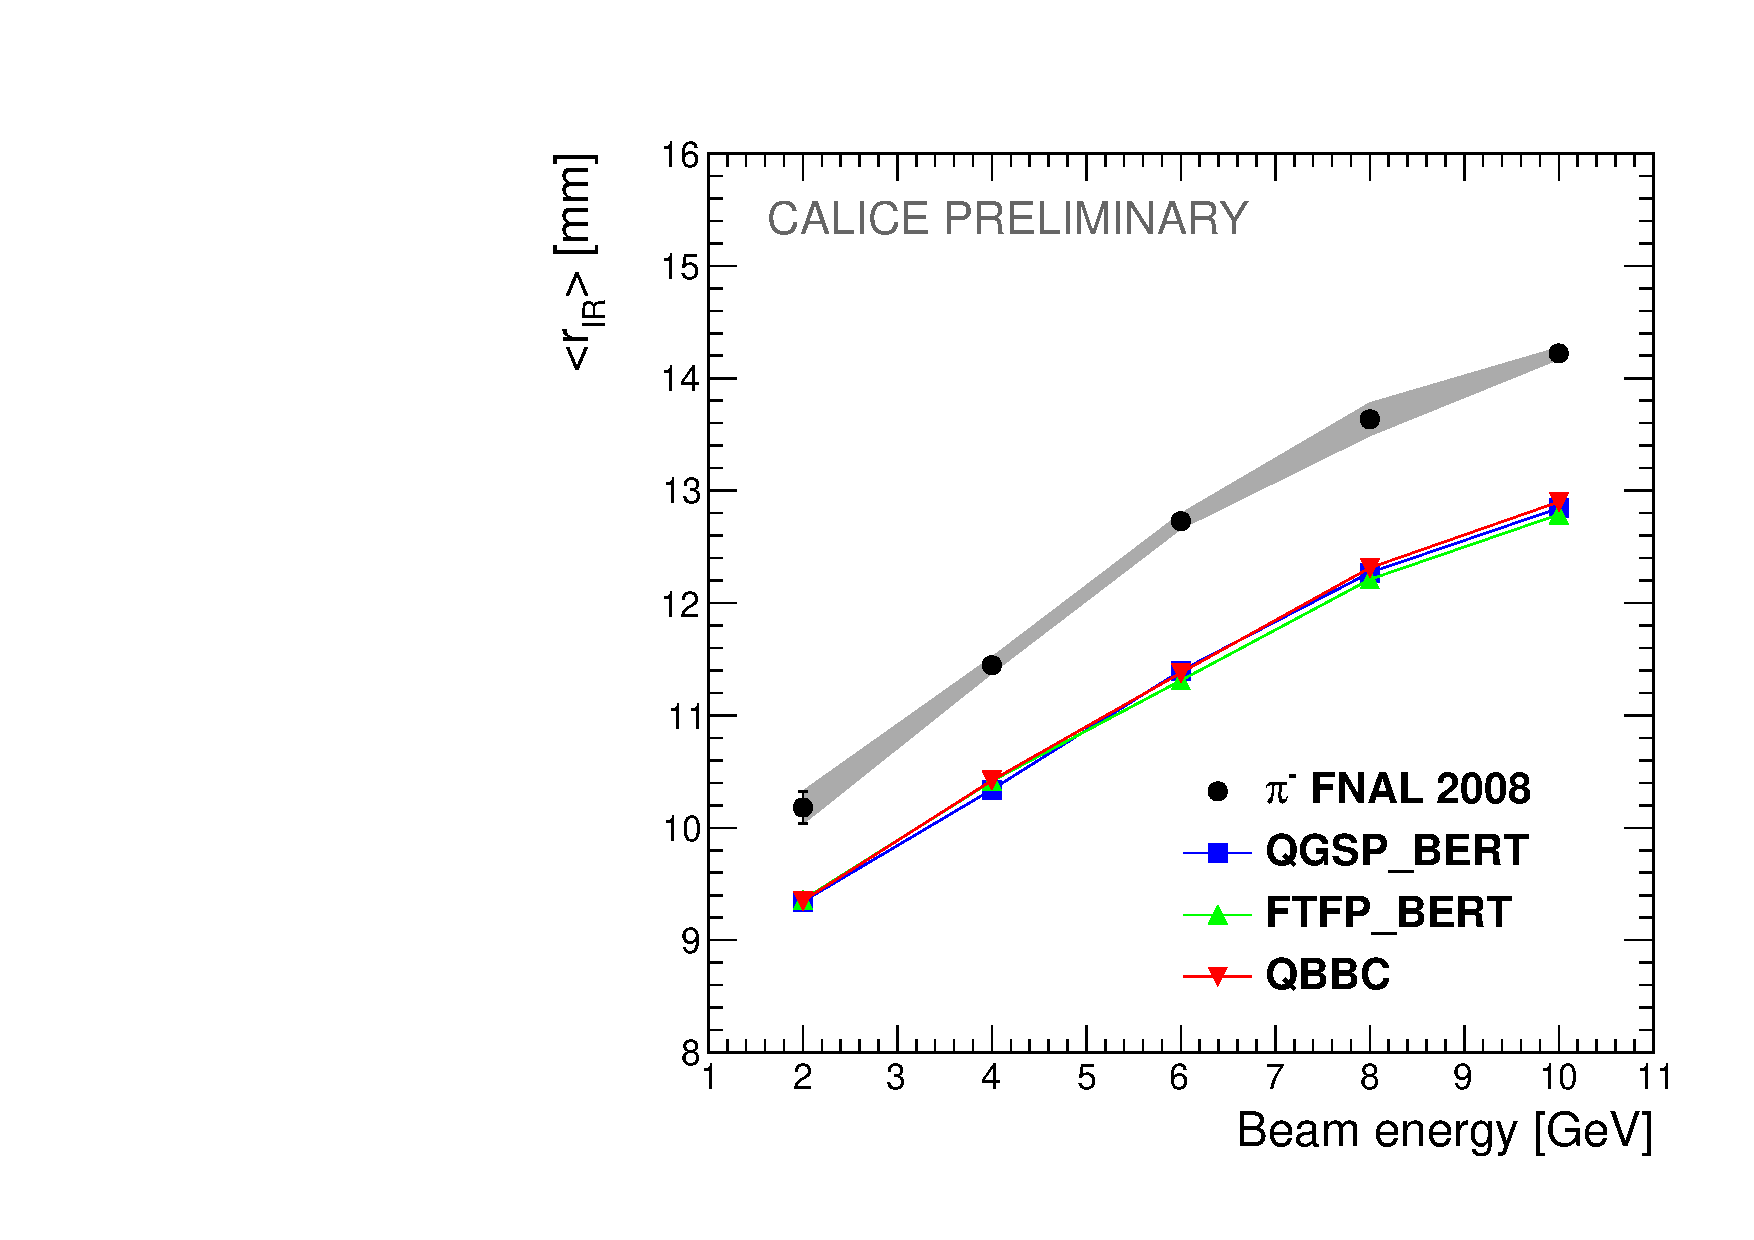
\includegraphics[width=0.5\textwidth]{ECAL/plots/r-ir-graph.pdf}
	\caption{\label{fig:irrgraph} \sl Mean $r_{IR}$ for data and Monte Carlo simulations for two {\sc Geant}4 physics lists as a function of the beam energy. Events without a detected interaction region according to Sec.~\ref{sec:iazone} are discarded. Error bars represent statistical uncertainties only and the error band the systematic error from the correction for double $\pi$ events.}
\end{figure}

%|||||||||||||||||||Number of clusters||||||||||||||||||||||
\subsection{Number of clusters}
As the final tracks are composed from segments that are given by clusters according to Sec.~\ref{sec:cluster}, it is instructive to study the total number of clusters ($N_{clusters}$) detected by the \tfa\ in the event. This observable is stable against details of the \tfa\,
since it does not depend neither on the \ep\ value nor on other free parameters of the classification algorithm. Here and in all of the following events without a detected interaction region according to Sec.~\ref{sec:iazone} are discarded.
The $N_{clusters}$ distribution is given in Fig. \ref{fig:clusterexample} for data and Monte Carlo simulation for the three {\sc Geant4} physics lists for energies of 2 and 10\,GeV of the incoming $\pi^-$-meson, respectively. The measured distributions are slightly shifted towards higher values with respect to those obtained for the three {\sc Geant4} physics lists.
%While the data and MC agree in many bins within errors, the distributions are nevertheless slightly shifted w.r.t. each other.  

Figure \ref{fig:clustergraph} shows the dependence of $\left<N_{clusters}\right>$  on different beam energies for data, \ftfp\ and \qgsp\ Monte Carlo simulations. At all energies the data are systematically above the Monte Carlo predictions with deviations of up to 7\%. The agreement tends to improves with increasing energy of the primary particle and is best at 10\,GeV. 
%At 2 and 10\,GeV there is a good agreement between data and both simulation samples, but for intermediate beam energies the \tfa\ tends to find more clusters in data than in Monte Carlo.
\begin{figure}
	\centering
	\begin{subfigure}{0.5\textwidth}
		\centering
		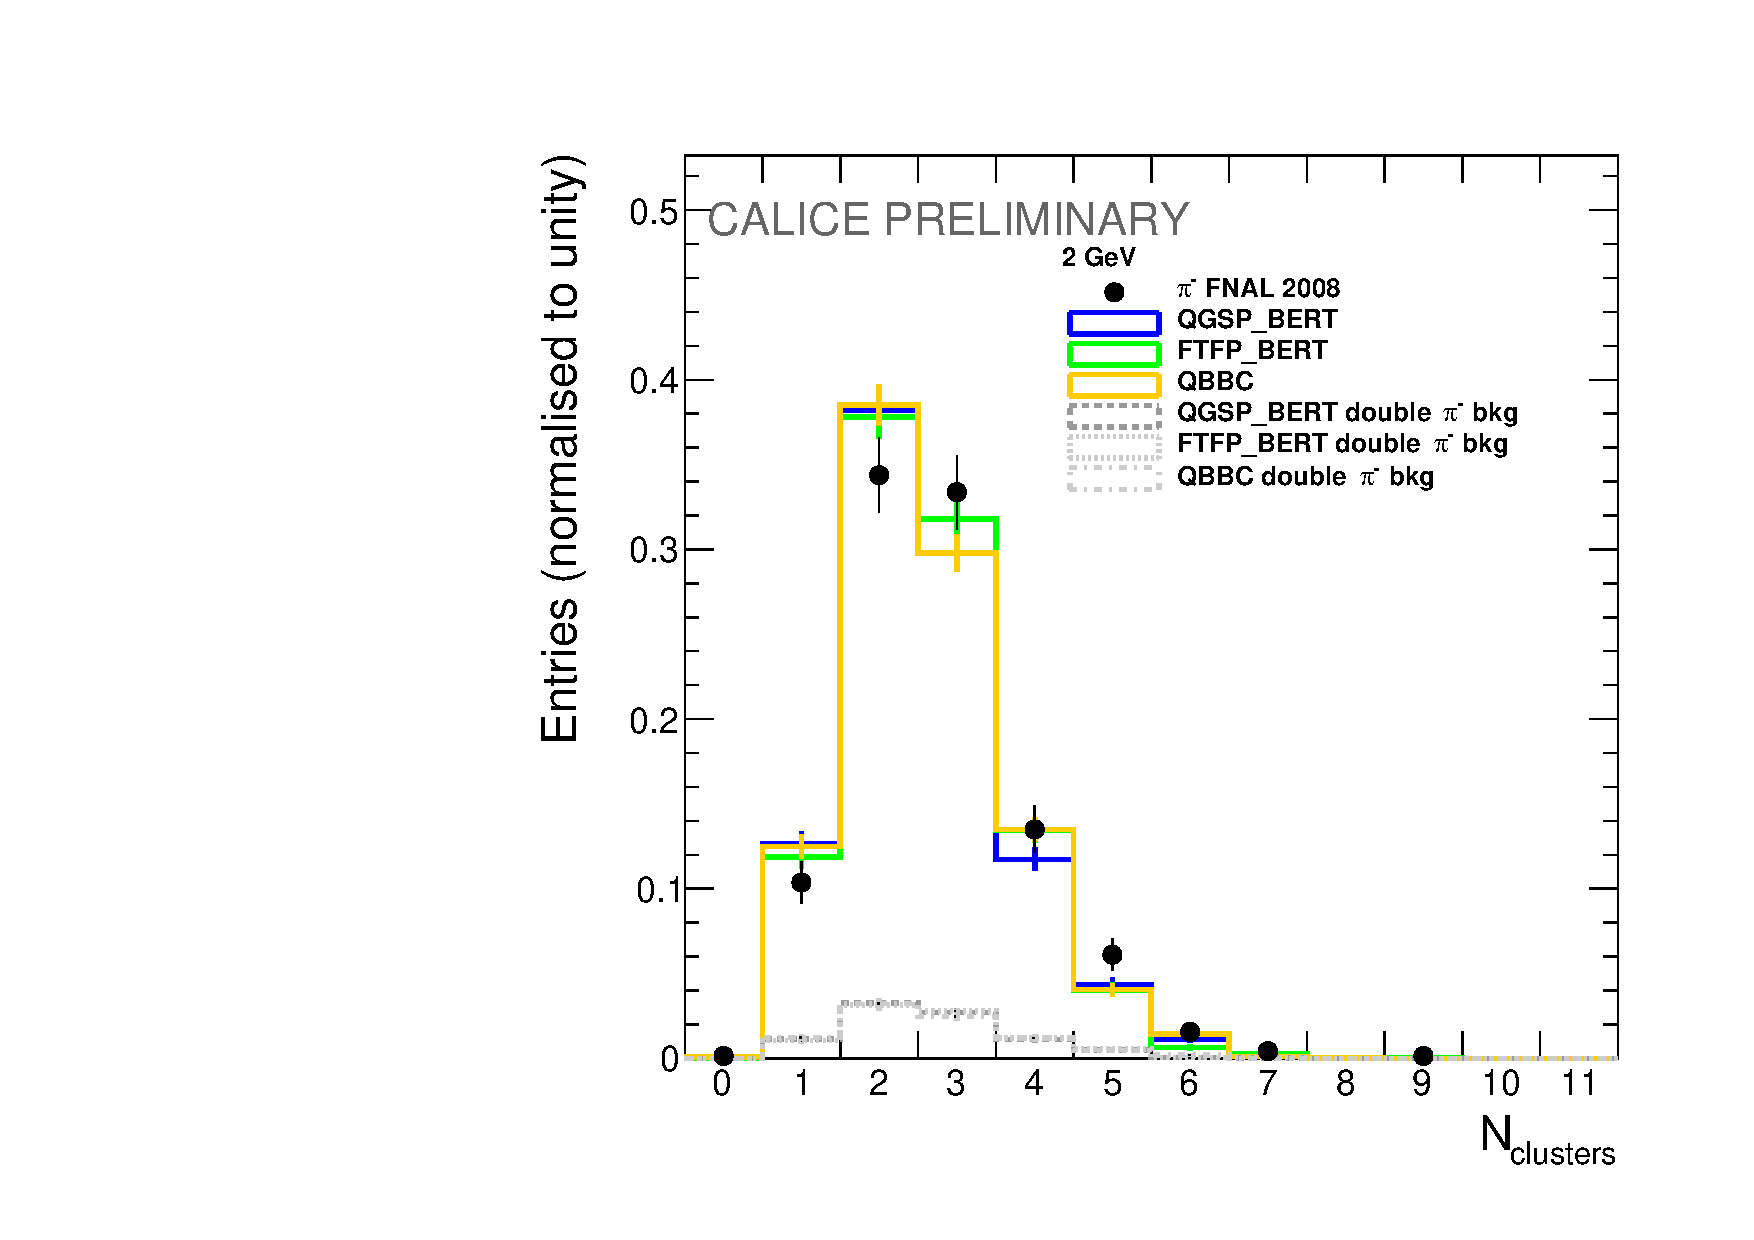
\includegraphics[width=.90\linewidth]{ECAL/plots/cluster-2.pdf}
		\caption{\label{fig:cl2} }
	\end{subfigure}% 
	\begin{subfigure}{0.5\textwidth}
		\centering
		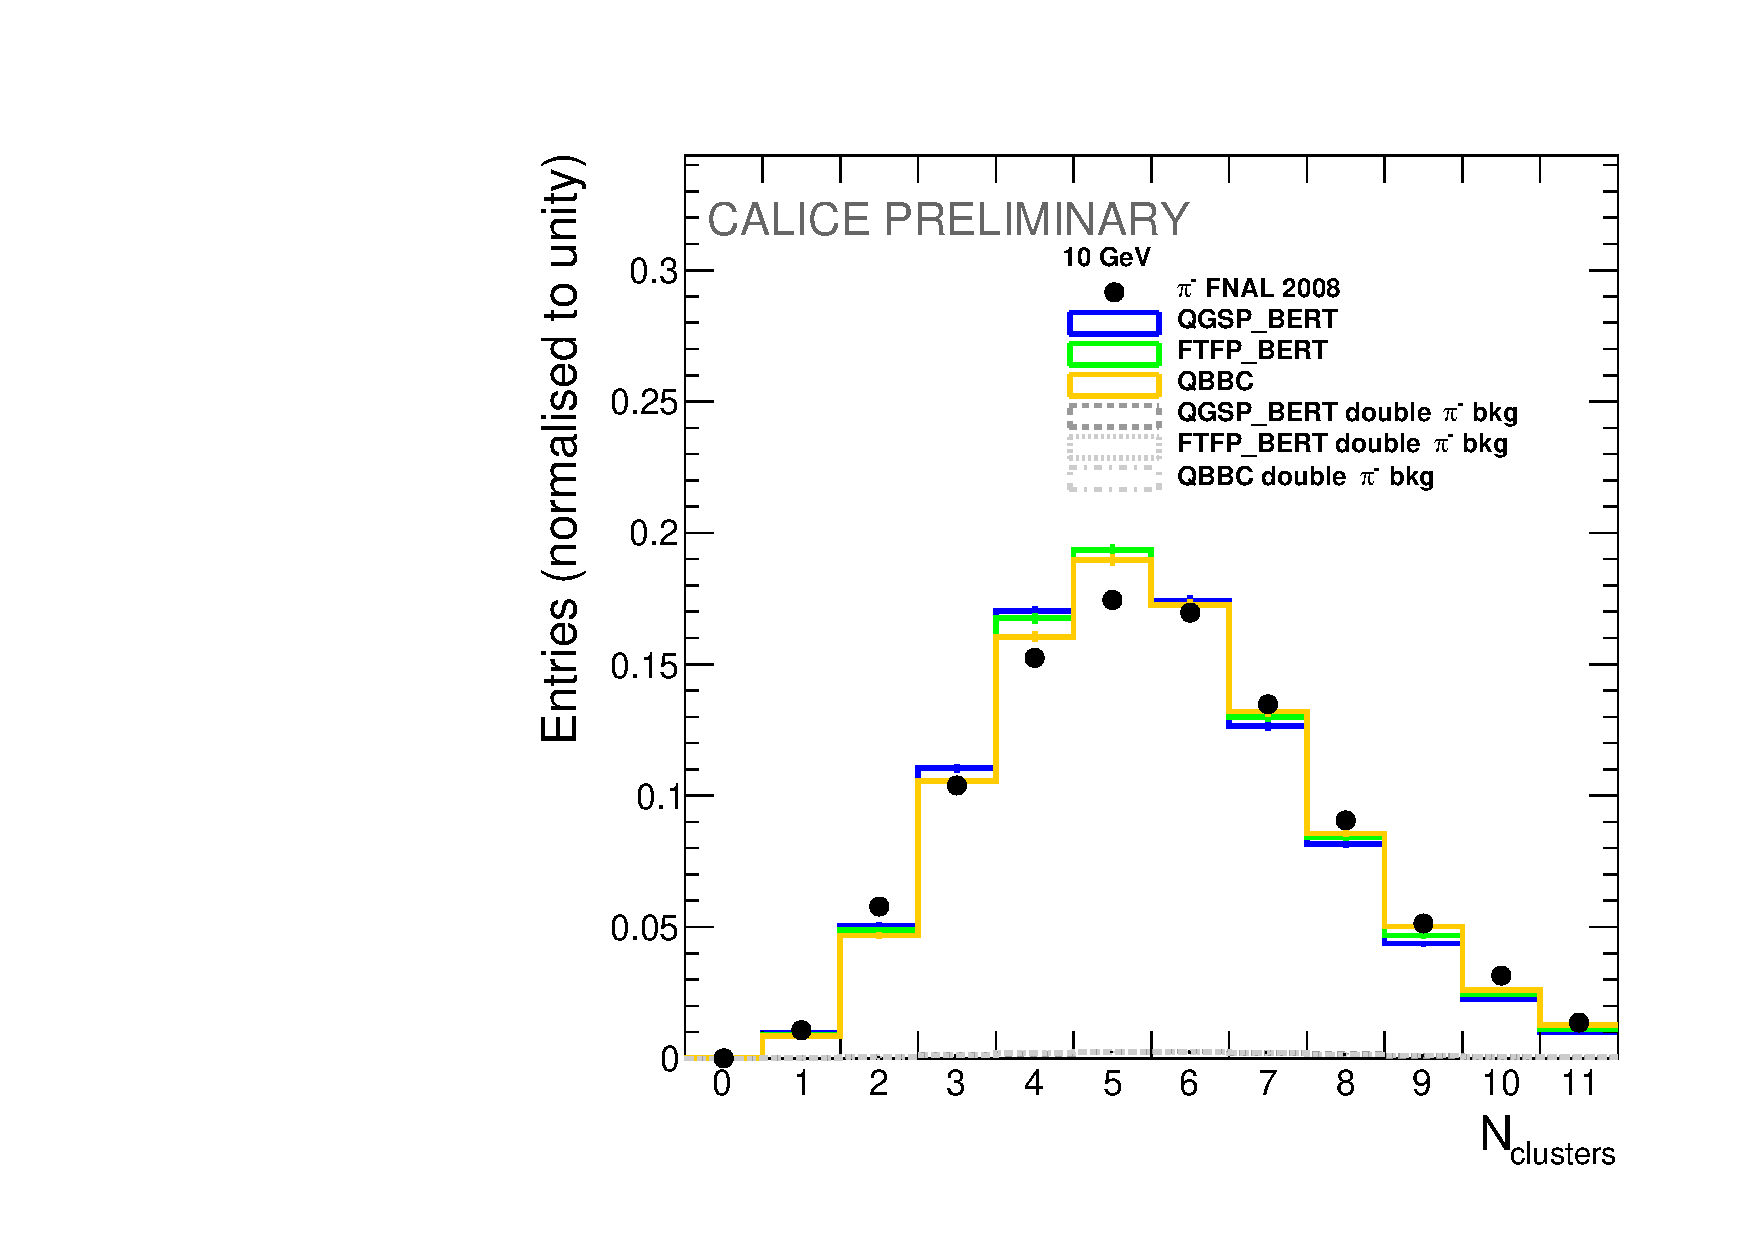
\includegraphics[width=.90\linewidth]{ECAL/plots/cluster-10.pdf}
		\caption{\label{fig:cl10} }
	\end{subfigure}
	\caption{\label{fig:clusterexample} \sl Comparison of the number of clusters found between data and Monte Carlo simulations for two {\sc Geant}4 physics lists for energies of the primary particle of 2 (a) and 10 (b) GeV, respectively. Events without a detected interaction region according to Sec.~\ref{sec:iazone} are discarded. Error bars represent statistical uncertainties only.}
\end{figure}

\begin{figure}
	\centering
	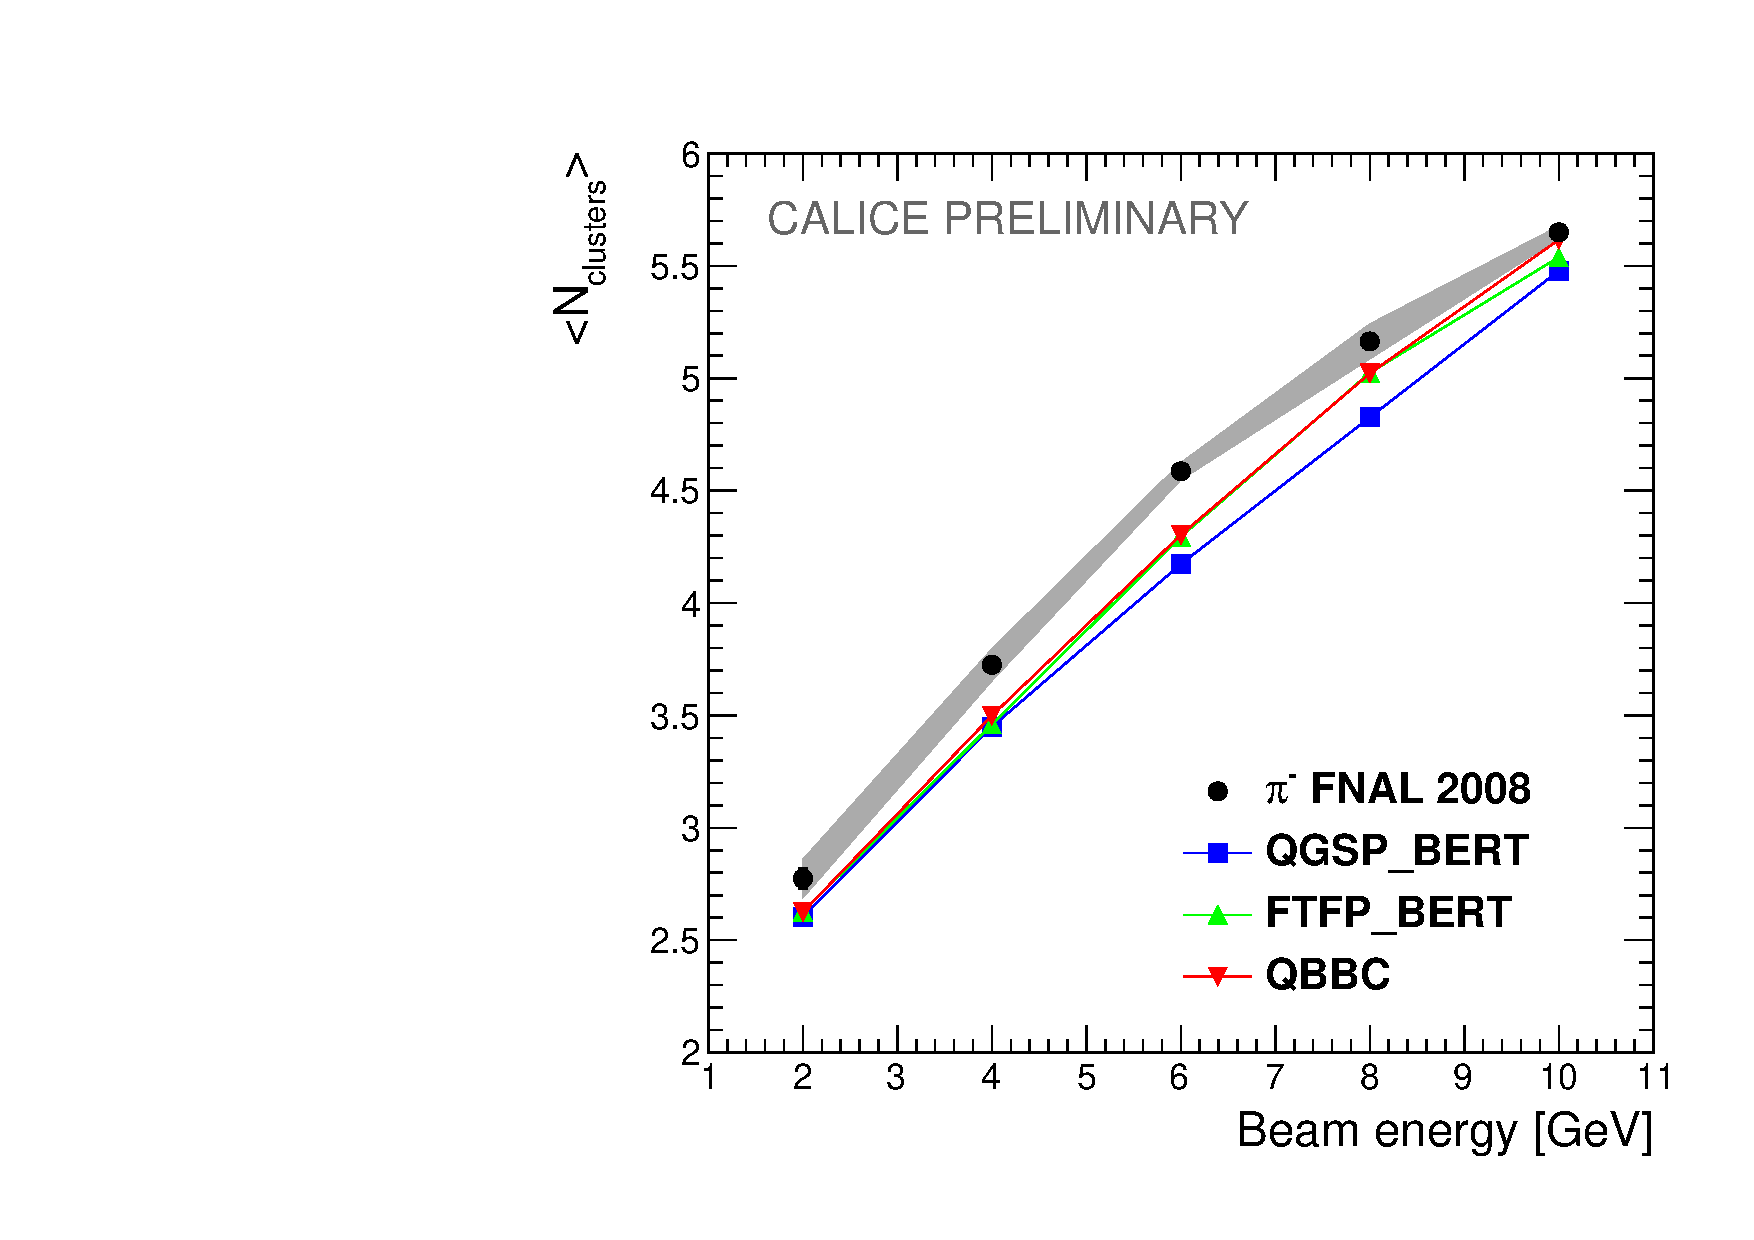
\includegraphics[width=0.5\textwidth]{ECAL/plots/cluster-graph.pdf}
	\caption{\label{fig:clustergraph} \sl Mean number of clusters in the \ecal\ for data and  Monte Carlo simulations for two {\sc Geant}4 physics lists as a function of beam energy (2\,GeV to 10\,GeV). Events without a detected interaction region according to Sec.~\ref{sec:iazone} are discarded. Error bars on the graph represent statistical uncertainties and the error band the systematic error from the correction for double $\pi$ events.}
\end{figure}

%||||||||||||||||||||Number of tracks||||||||||||||||||||||||
\subsection{Number of tracks}
A central result of the \tfa\ is the number of secondary tracks ($N_{tracks}$) and observables based on their properties.
The $N_{tracks}$ distributions are given in Fig. \ref{fig:trackexample} for data and Monte Carlo simulations based on the three tested {\sc Geant4} physics lists for energies of 2 and 10\,GeV of the incoming $\pi^-$-mesons. A remarkably good agreement between data and both physics lists can be reported, given the fact that this observable is analysed for the first time in the \ecal. 

Figure \ref{fig:tracksgraph} shows the dependence of $\left<N_{tracks}\right>$ on the beam energy for data and the three {\sc Geant4} physics lists. 
Both physics lists, presented in Fig.  \ref{fig:tracksgraph} underestimate the number of secondary tracks by 7\% on average below 10\,GeV and are in agreement with the data at 10\,GeV. 
%Both simulation samples are in agreement with data within systematic uncertainties here given by the variation of the \ep\ according to $\varepsilon = 0.03 \pm 0.01$.

%As a measure for the sensitivity of the reconstructed number of tracks on the actual value of the \ep, the estimator 
%\begin{equation}
%\Delta {\cal O} = < {\cal O}(\varepsilon_{up}) - {\cal O}(\varepsilon_{low}> /{\cal O}(\varepsilon_{nom} = 0.03)>
%\end{equation}
%is introduced
The sensitivity to the \ep\ defined by Eq.~\ref{eq:sens} for ${\cal O}=N_{tracks}$, $\varepsilon_{1},=0.04$, $\varepsilon_{2},=0.02$ and $\varepsilon_{nom.}=0.03$   
%$\Delta N_{tracks} = <N_{tracks}(\varepsilon = 0.04) - N_{tracks}(\varepsilon = 0.02)> /<N_{tracks}(\varepsilon = 0.03)> $ is used. 
is shown in Fig. \ref{fig:dtracksgraph}. Within the chosen range the number of reconstructed tracks varies by about 10\% for both, data and the three {\sc Geant4} physics lists. 
\begin{figure}
	\centering
	\begin{subfigure}{0.5\textwidth}
		\centering
		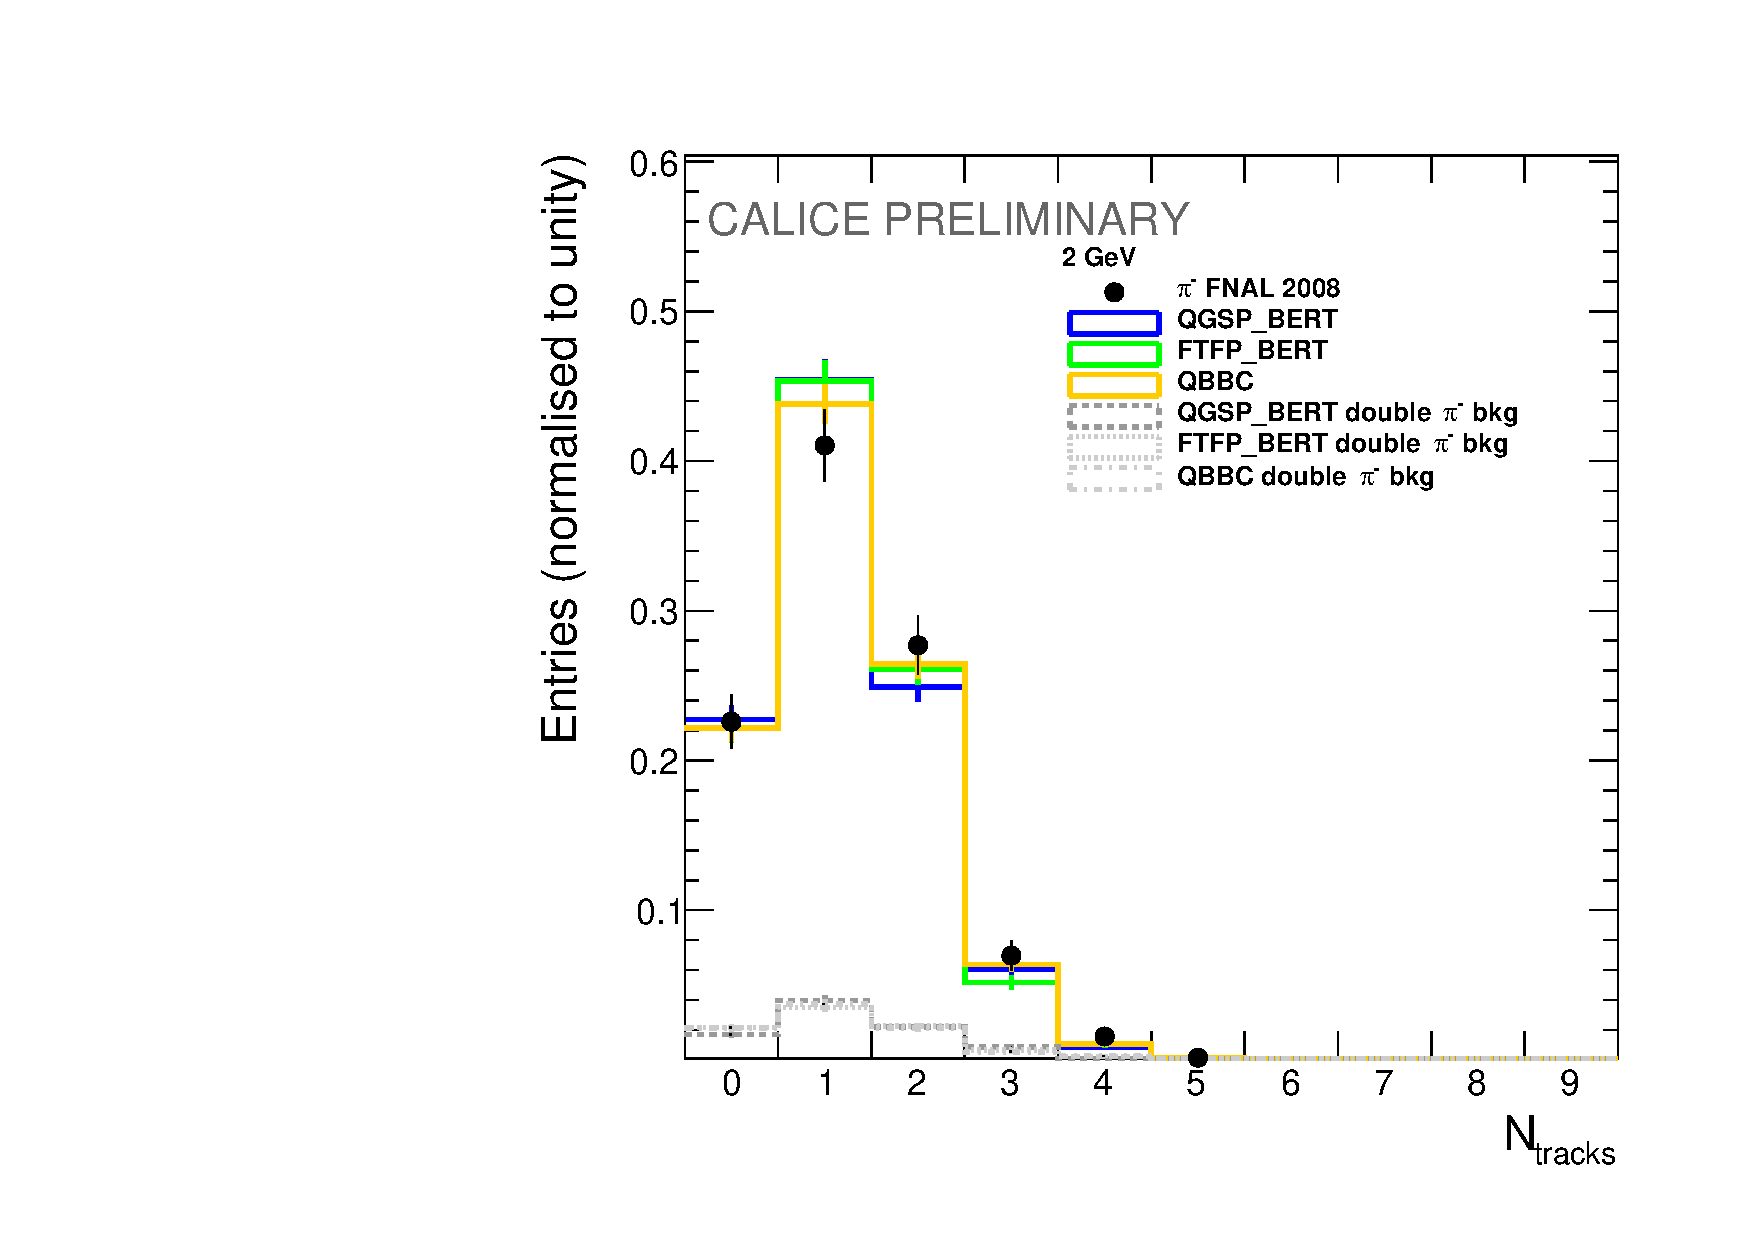
\includegraphics[width=.90\linewidth]{ECAL/plots/ntracks-2.pdf}
		\caption{\label{fig:tr2} }
	\end{subfigure}% 
	\begin{subfigure}{0.5\textwidth}
		\centering
		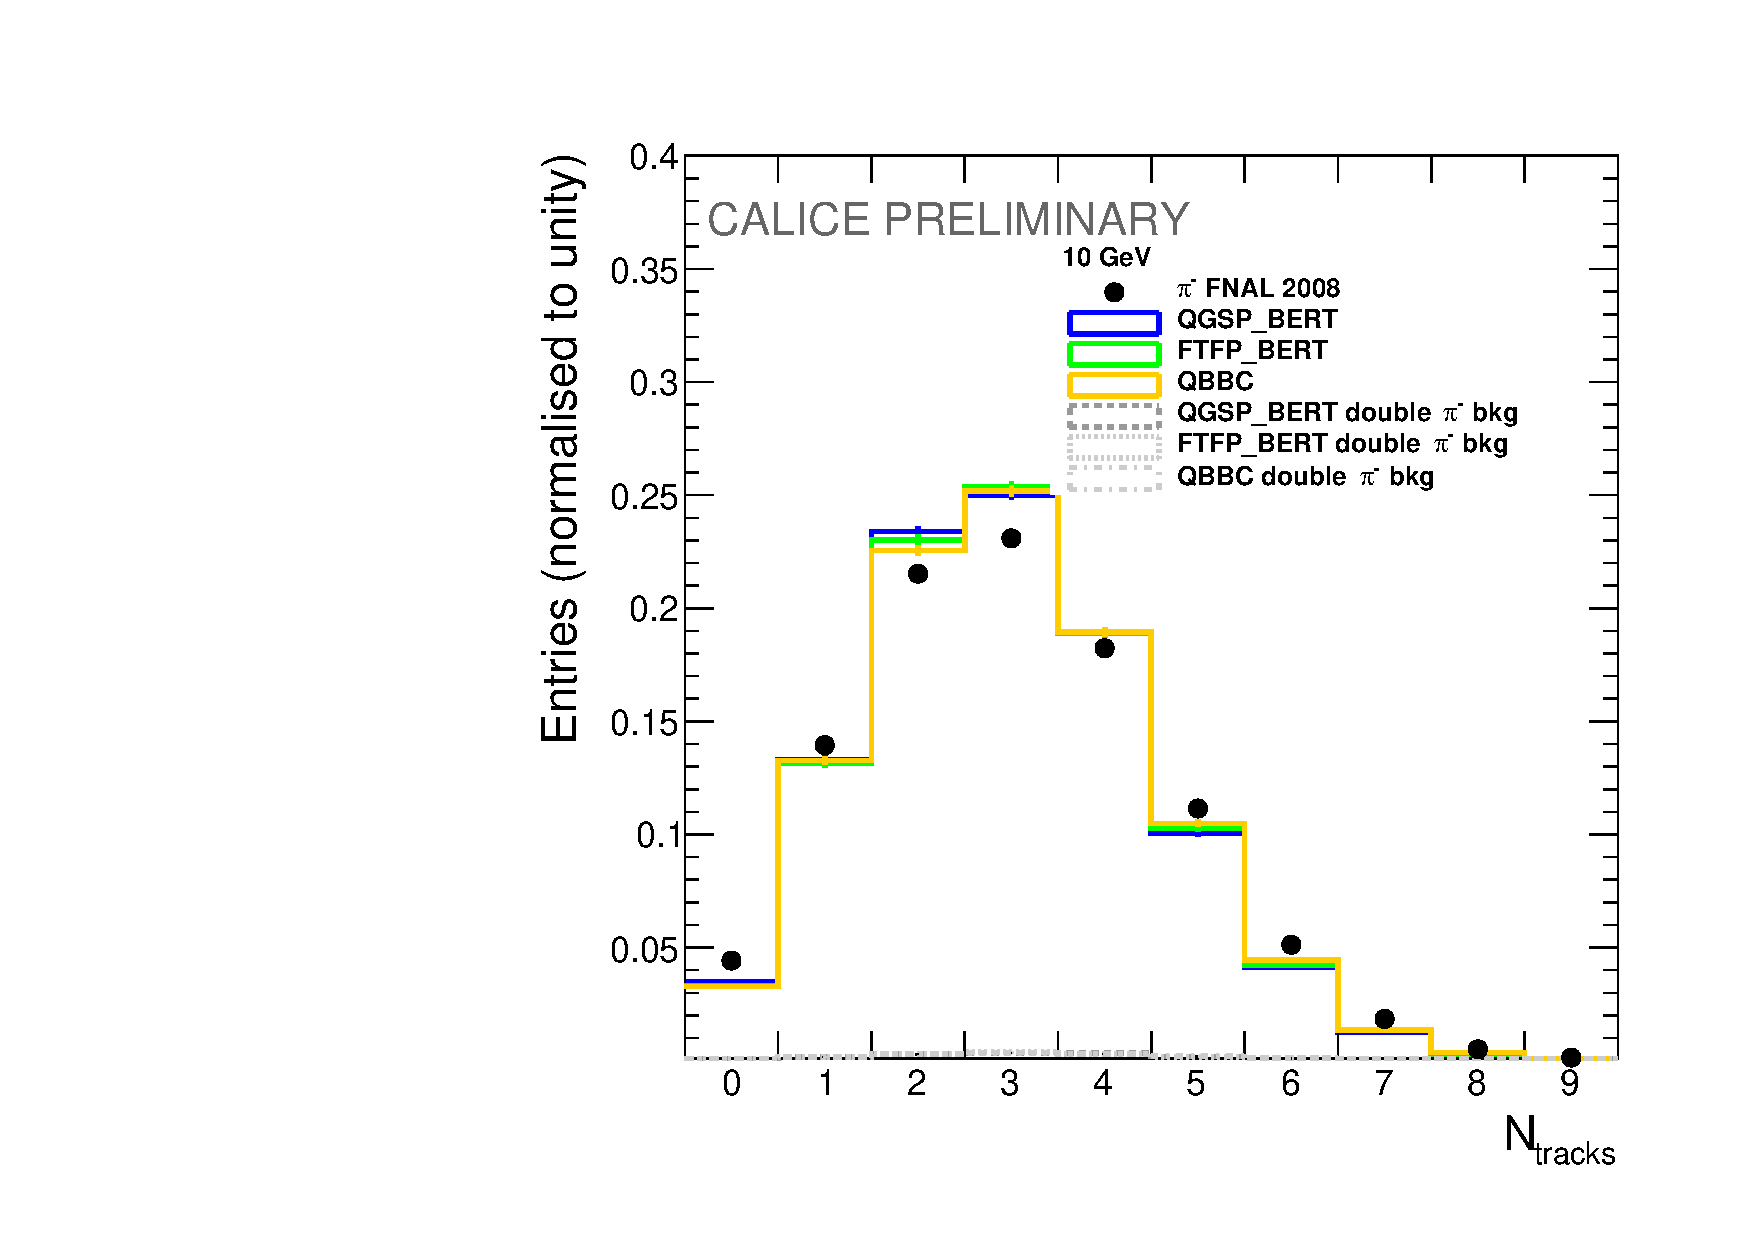
\includegraphics[width=.90\linewidth]{ECAL/plots/ntracks-10.pdf}
		\caption{\label{fig:tr10} }
	\end{subfigure}
	\caption{\label{fig:trackexample} \sl Comparison of the number of secondary tracks between data Monte Carlo simulations for two {\sc Geant}4 physics lists  for energies of the primary particle of 2 (a) and 10 (b) GeV. Events without a detected interaction region according to Sec.~\ref{sec:iazone} are discarded. Error bars represent statistical errors only.}
\end{figure}

\begin{figure}
	\centering
	\begin{subfigure}{0.5\textwidth}
		\centering
		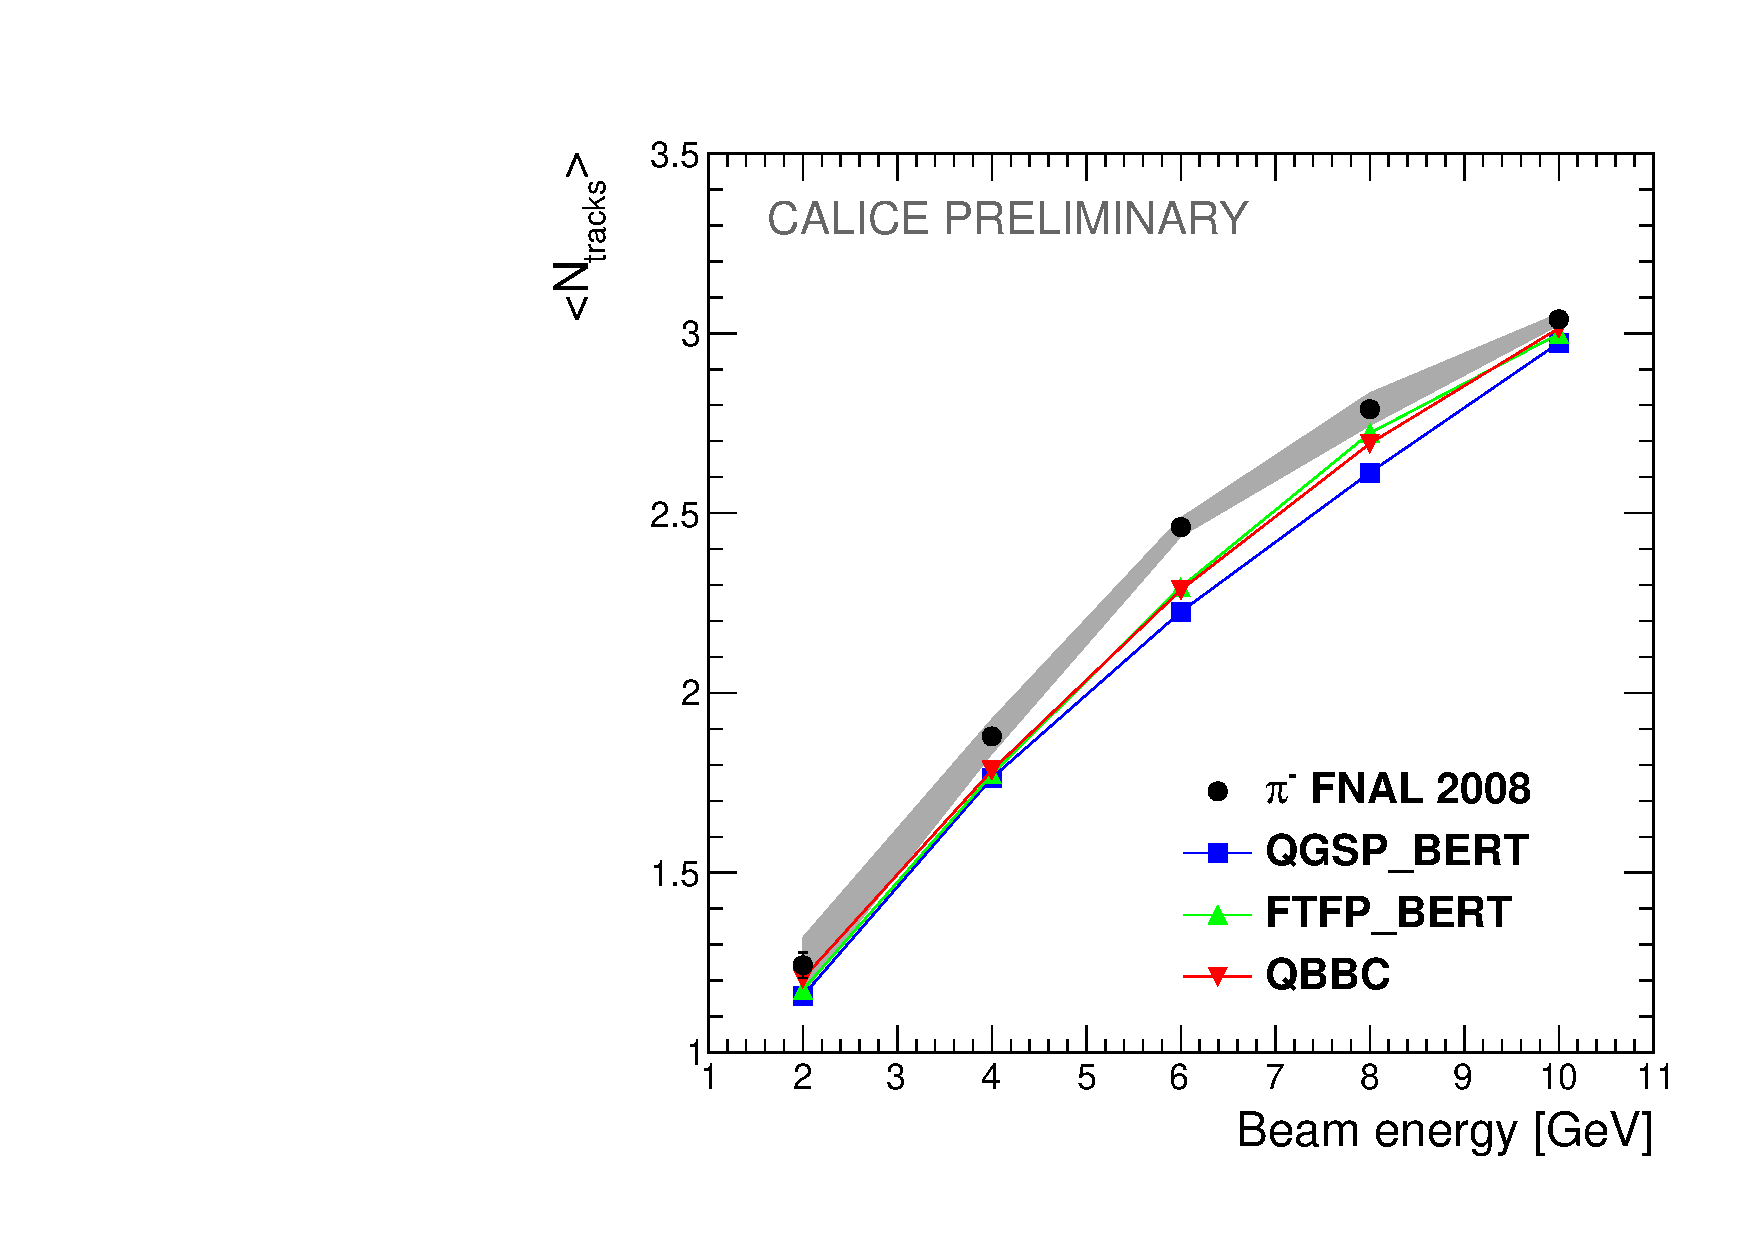
\includegraphics[width=.90\linewidth]{ECAL/plots/ntracks-graph.pdf}
		\caption{\label{fig:tracksgraph} }
	\end{subfigure}% 
	\begin{subfigure}{0.5\textwidth}
		\centering
		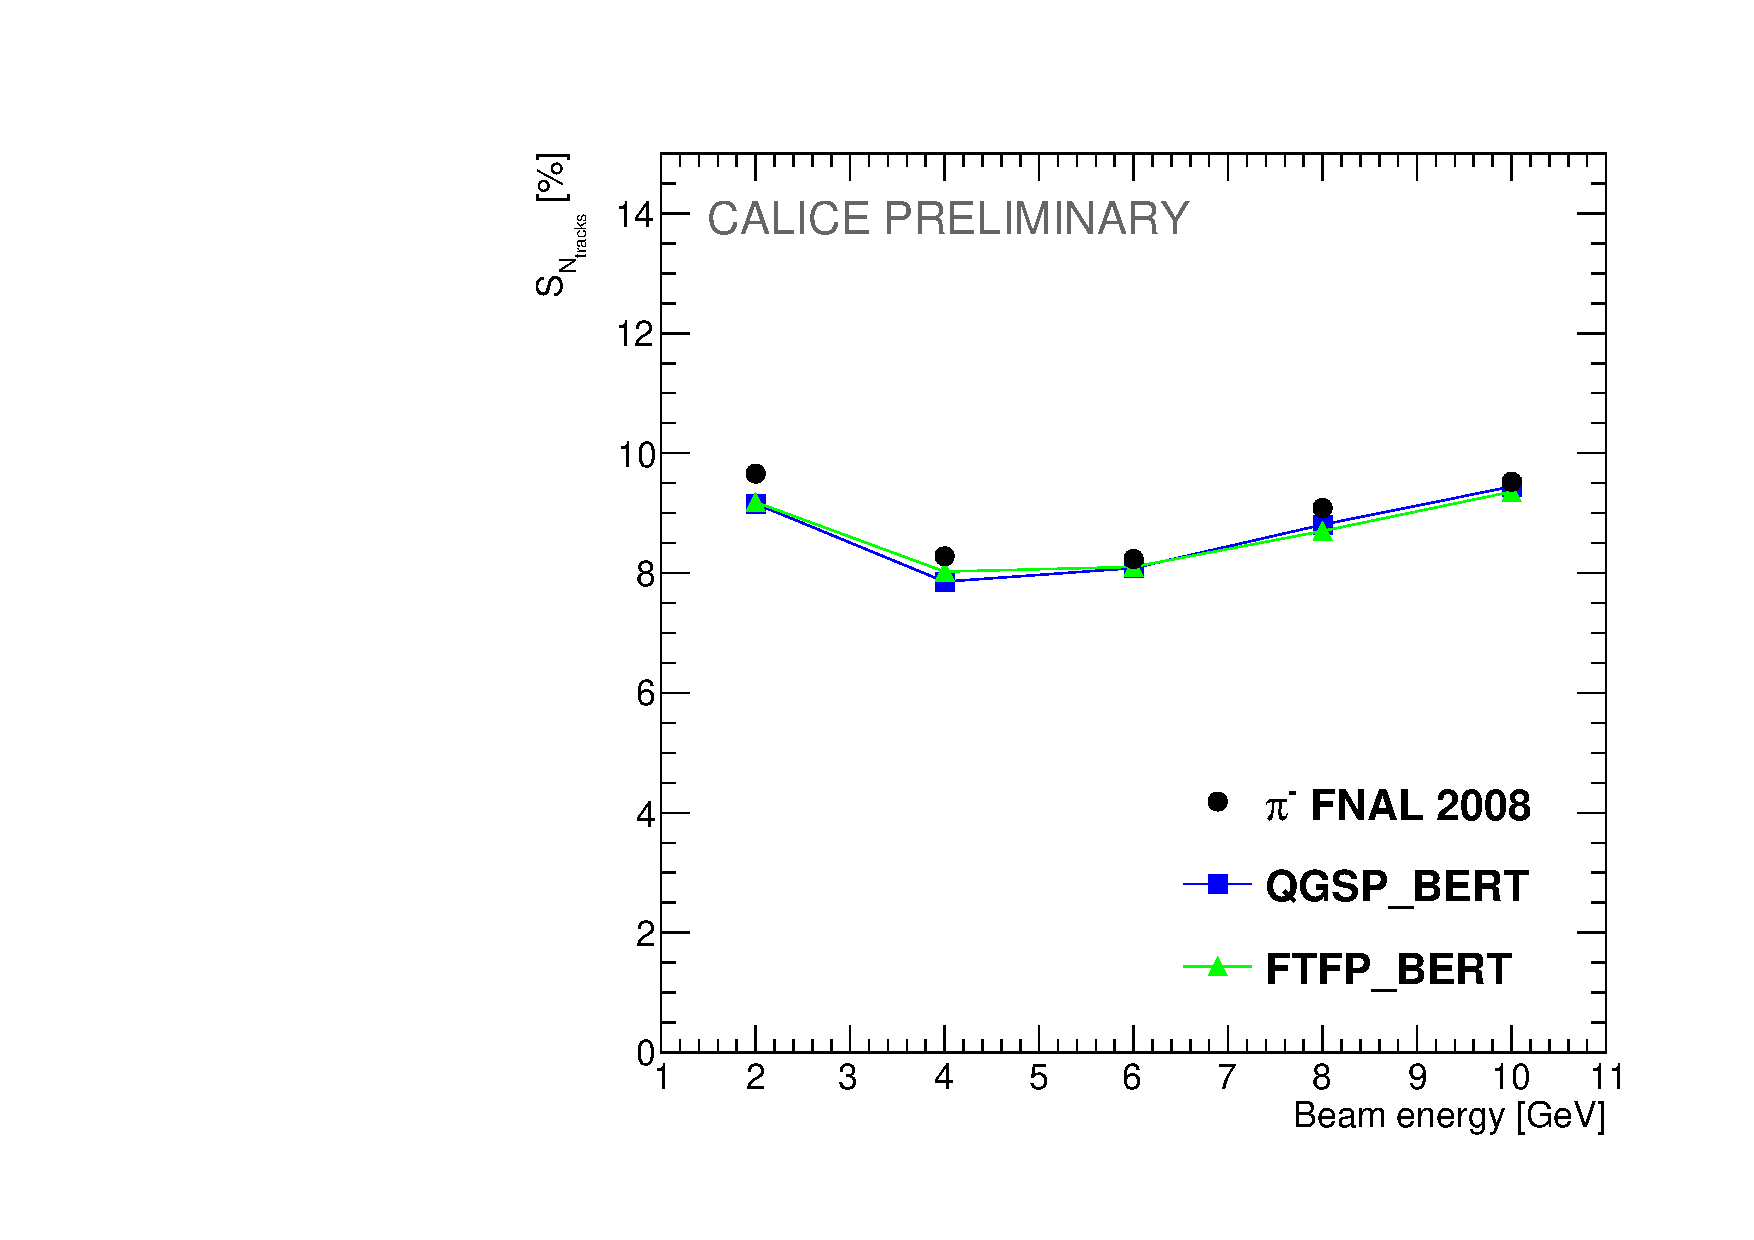
\includegraphics[width=.90\linewidth]{ECAL/plots/delta-ntracks-graph.pdf}
		\caption{\label{fig:dtracksgraph}}
	\end{subfigure}
	\caption{\label{fig:fulltrackgraph} \sl Mean number of secondary tracks $\left<N_{tracks}\right>$ for $\varepsilon = 0.03$ (a) and the corresponding sensitivity according to Eq.~\ref{eq:sens} of $\left<N_{tracks}\right>$ on the \ep\,(b) for data and Monte Carlo simulations for two {\sc Geant}4 physics lists as a function of the beam energy (from 2 to 10\,GeV). The sensitivity, see Eq.~\ref{eq:sens}, is estimated by the mean difference in $N_{tracks}$ for $\varepsilon_1 = 0.04$ and $\varepsilon_2 = 0.02$ normalised to the result for $\varepsilon_{nom} = 0.03$. Events without a detected interaction region according to Sec.~\ref{sec:iazone} are discarded. Error bars represent statistical errors and the error band the systematic error from the correction for double $\pi$ events.}
\end{figure}

%|||||||||||||||||||||Hit distribution||||||||||||||||||||||


\subsection{Number of hits per track}
The number of hits per track $N_{hits}^t$ is an essential feature to characterise the reconstructed tracks. 
The histograms of $N_{hits}^t$ for 2 and 10\,GeV beam energy are shown in Fig. \ref{fig:trackhitsexample}.
The distributions obtained for data and Monte Carlo agree in many bins within statistical errors and are therefore in good overall agreement with each other. 

Figure \ref{fig:trackshitsgraph} shows the dependence of $\left<N_{hits}^t\right>$ on the beam energy for data, \ftfp\ and \qgsp\ Monte Carlo simulations. The Monte Carlo models agree with the data within 5\%.  For energies greater than 4\,GeV both models are however systematically above  the data.
%The parametric uncertainty for the number of hits per track is defined as $\Delta N_{hits}^t = <N_{hits}^t(\varepsilon = 0.04) - N_{hits}^t(\varepsilon = 0.02)> /  <N_{hits}^t(\varepsilon = 0.03)>$. 
The sensitivity to the \ep\  as defined by Eq.~\ref{eq:sens} for ${\cal O}=N_{hits}$, $\varepsilon_{1},=0.04$, $\varepsilon_{2},=0.02$ and $\varepsilon_{nom.}=0.03$ is shown in Fig. \ref{fig:dtrackshitsgraph}. For the chosen parameter range the sensitivity increases with increasing beam energy from 1\% to about 5\% for both, data and the three {\sc Geant4} physics lists. 
%Figure \ref{fig:dtrackshitsgraph} demonstrates a similar behavior of parametric uncertainty on $N_{hits}^t$ for data and Monte Carlo. 

\begin{figure}
	\centering
	\begin{subfigure}{0.5\textwidth}
		\centering
		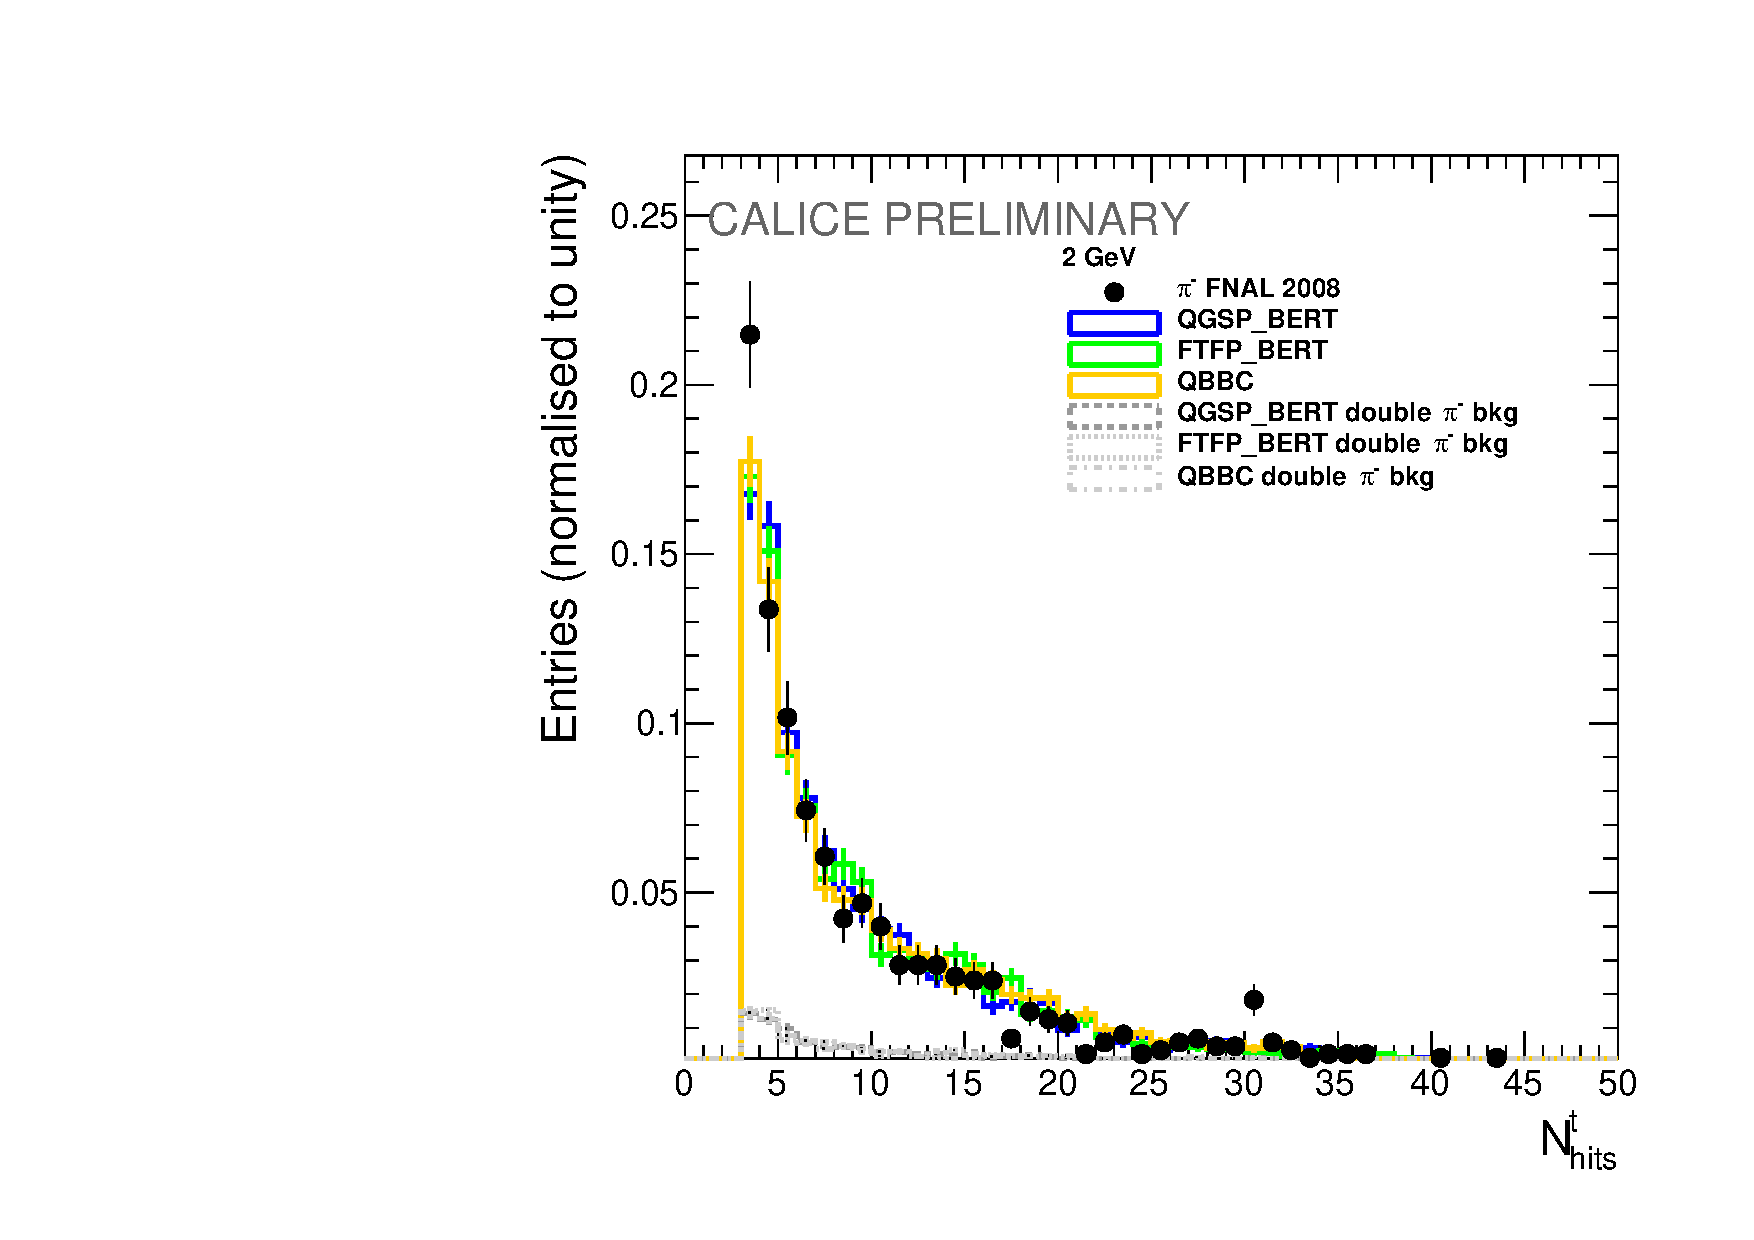
\includegraphics[width=.90\linewidth]{ECAL/plots/number-2.pdf}
		\caption{\label{fig:trh2} }
	\end{subfigure}% 
	\begin{subfigure}{0.5\textwidth}
		\centering
		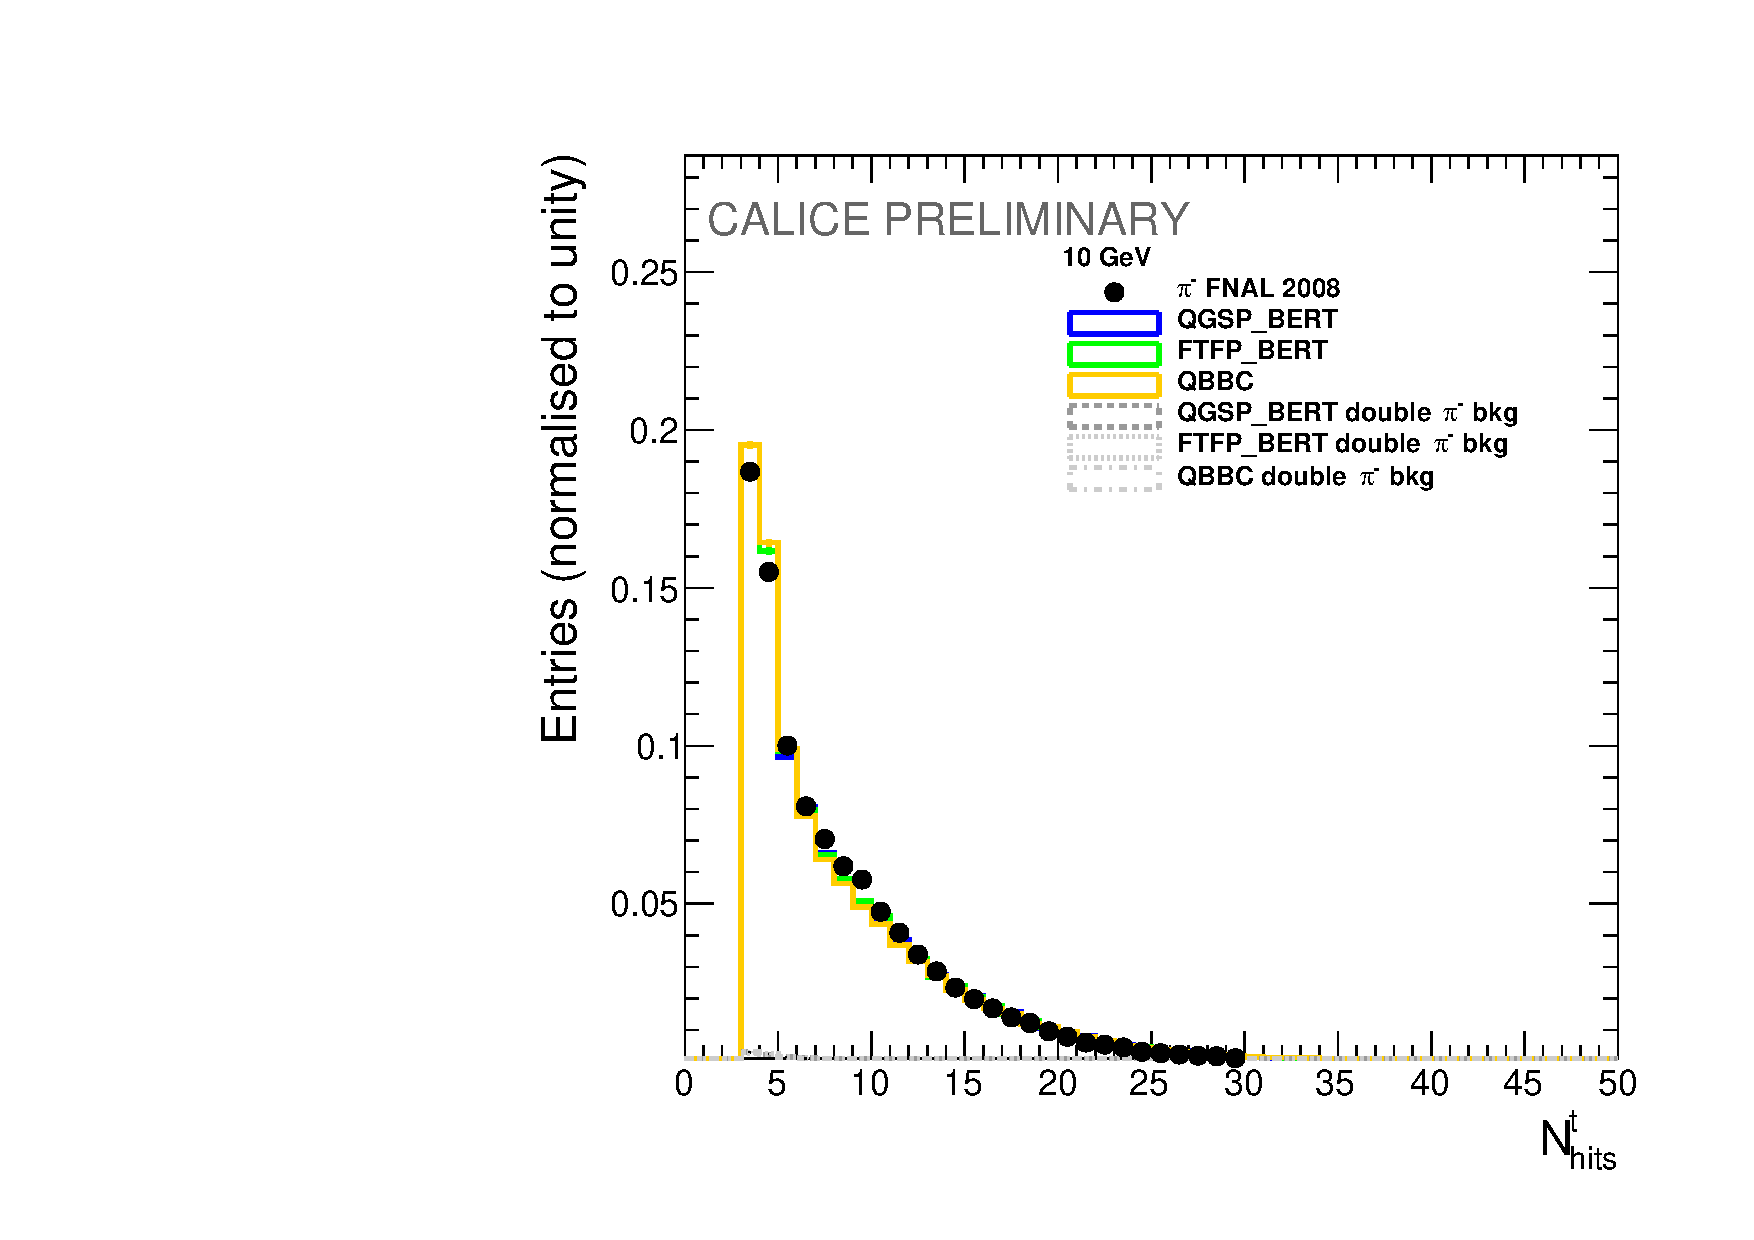
\includegraphics[width=.90\linewidth]{ECAL/plots/number-10.pdf}
		\caption{\label{fig:trh10} }
	\end{subfigure}
	\caption{\label{fig:trackhitsexample} \sl A comparison of the number of hits per reconstructed track between data and Monte Carlo simulations for two {\sc Geant}4 physics lists  or energies of the primary particle of 2 (a) and 10 (b) GeV, respectively. Events without a detected interaction region according to Sec.~\ref{sec:iazone} are discarded. The distributions are normalised to unity. Error bars represent statistical uncertainties only.}
\end{figure}

\begin{figure}
	\centering
	\begin{subfigure}{0.5\textwidth}
		\centering
		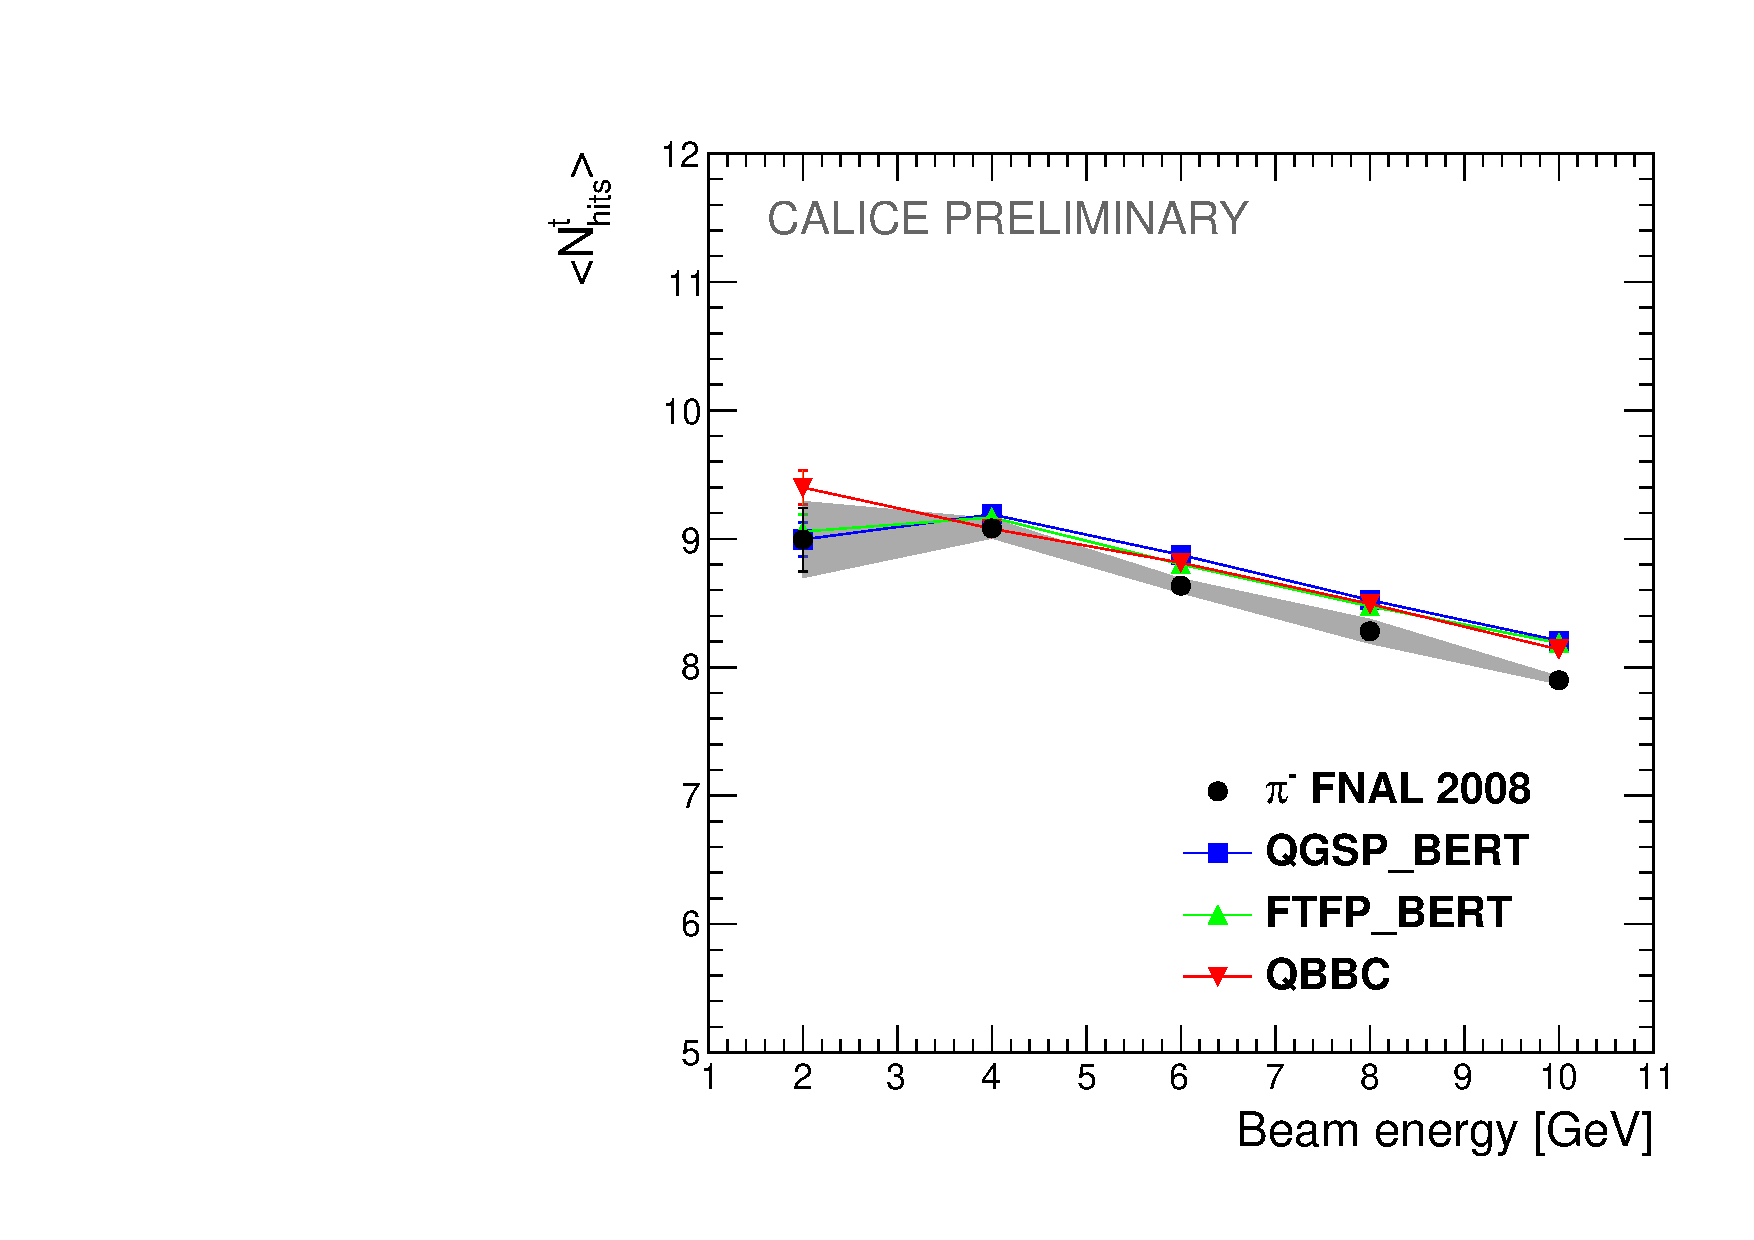
\includegraphics[width=.90\linewidth]{ECAL/plots/number-graph.pdf}
		\caption{\label{fig:trackshitsgraph}}
	\end{subfigure}% 
	\begin{subfigure}{0.5\textwidth}
		\centering
		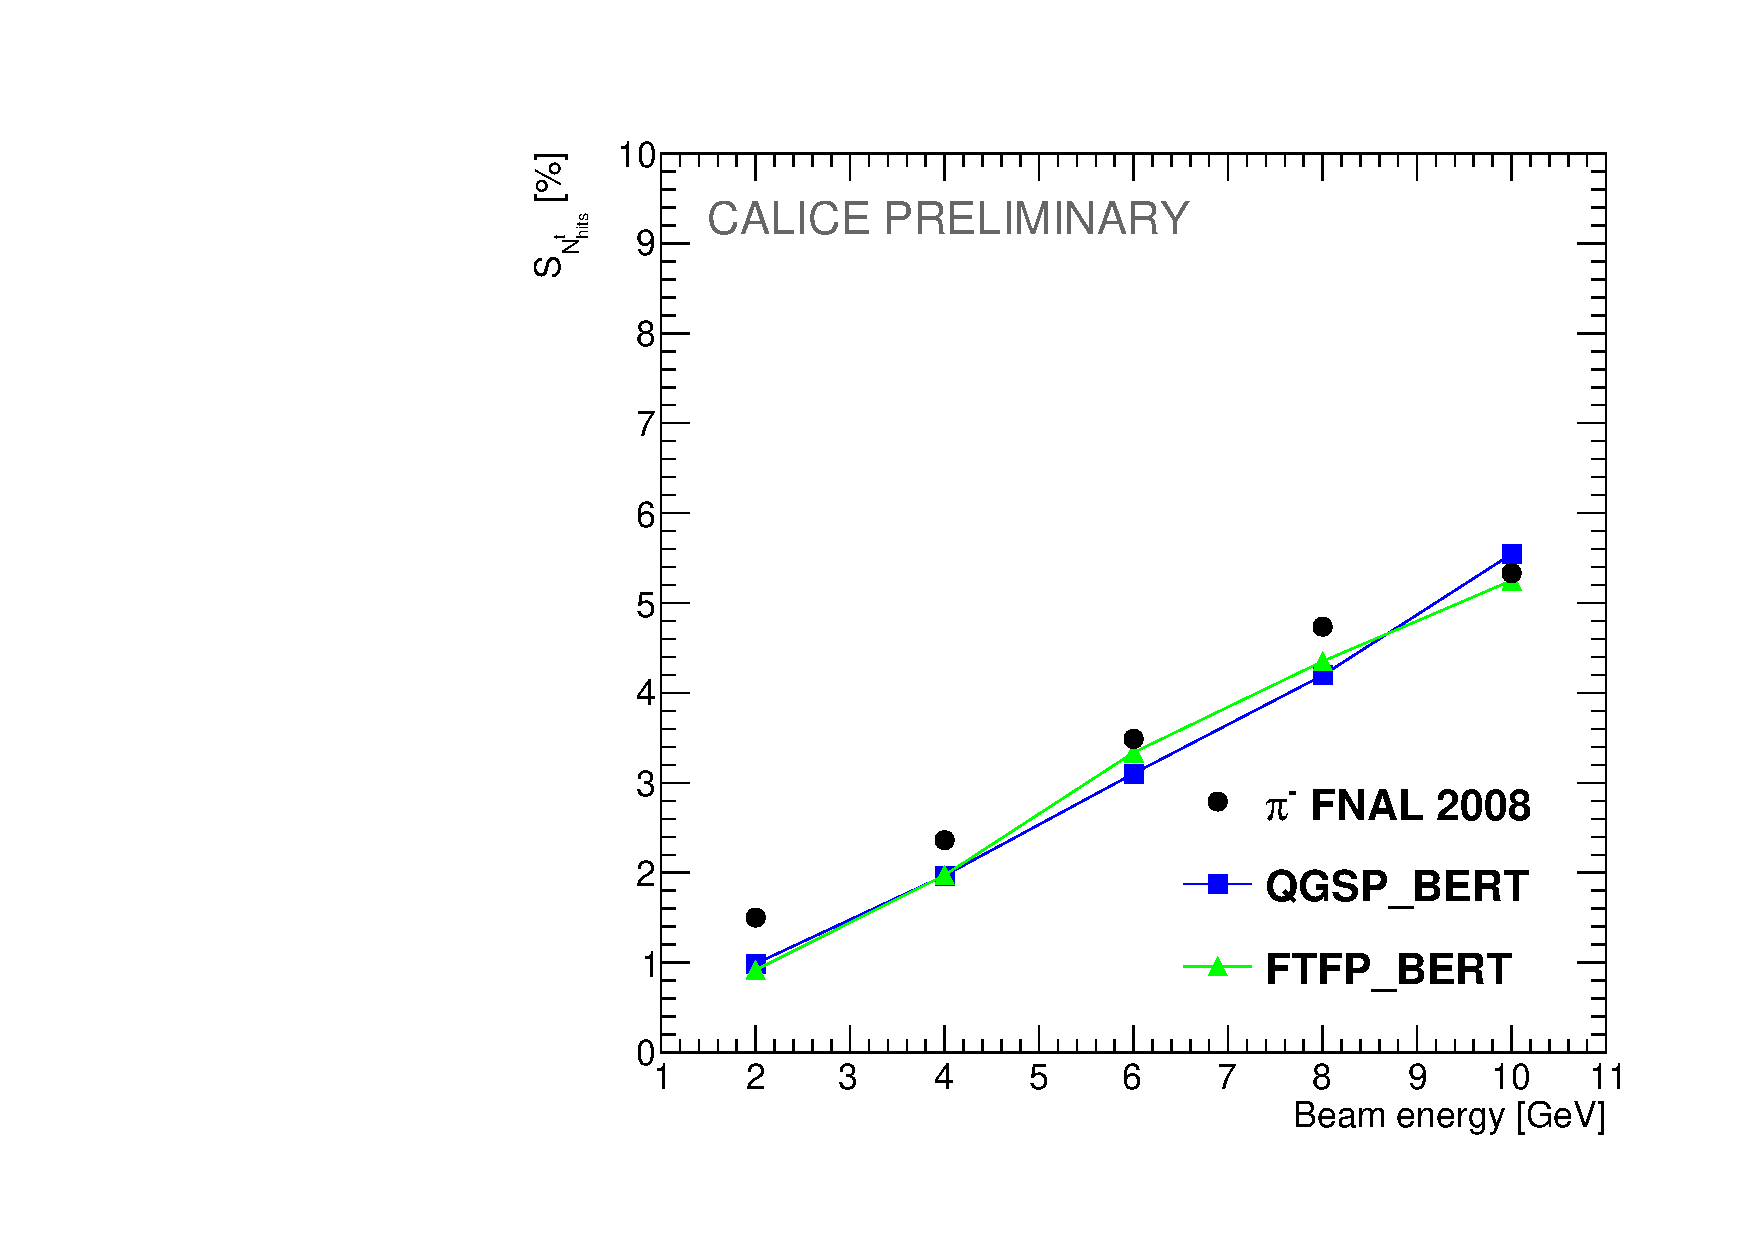
\includegraphics[width=.90\linewidth]{ECAL/plots/delta-number-graph.pdf}
		\caption{\label{fig:dtrackshitsgraph}}
	\end{subfigure}
	\caption{\label{fig:fulltrackhitsgraph} \sl Mean number of hits per reconstructed track  $\left<N_{hits}^t\right>$ for $\varepsilon = 0.03$  (a) and the corresponding sensitivity according to Eq.~\ref{eq:sens} of  $\left<N_{hits}^t\right>$ on the \ep\, (b) for data and Monte Carlo simulations for two {\sc Geant}4 physics lists as a function of beam energy (from 2 to 10\,GeV). Events without a detected interaction region according to Sec.~\ref{sec:iazone} are discarded. The sensitivity, see Eq.~\ref{eq:sens}, is estimated by the mean difference in $N_{hits}^t$ for $\varepsilon_1 = 0.04$ and $\varepsilon_2 = 0.02$ normalised to the result for $\varepsilon_{nom} = 0.03$. Error bars represent statistical errors and the error band the systematic error from the correction for double $\pi$ events.}
\end{figure}


%|||||||||||||||||||Angular distribution||||||||||||||||||||
\subsection{Angular distributions}
Due to the high granularity of the \ecal\, further tracking observables as the polar ($\theta$) and azimuthal ($\phi$) angles of secondary tracks become available.
Without a magnetic field, the secondary particles from hadronic interaction undergo only multiple elastic scattering in the detector material. Therefore, the direction of the initial momentum coincides approximately with the direction of the track that is visible in the \ecal.
Both angles are measured with respect to the $z$-axis in the right-handed coordinate frame defined in Sec.~\ref{sec:fnal}. The track direction is calculated from the position of the first and last hit of the track along the $z$-axis. 

Figures \ref{fig:thetaexample} and \ref{fig:phiexample} display histograms of the $\theta$ and $\phi$ angles, respectively, for 2 and 10\,GeV data and simulations based on the \ftfp\ an \qgsp\ physics lists. 

When corrected for the staggering of the detector layers in $x$-direction~\cite{Anduze:2008hq}, the pad coordinates of the \ecal\ define a grid with a step width of about 1\,cm in lateral direction. 
%The \tfa\ produces tracks with start and end points that are fixed to discrete calorimeter hit coordinates. 
This leads to a discretisation of the measured track direction and, therefore, to the $\phi$ and $\theta$ distributions in Figs. \ref{fig:thetaexample} and \ref{fig:phiexample}. In particular, $\phi$, angles that are a multiple of $\phi/4$ are privileged.
For 2 and 10\,GeV beam energy the {\sc Geant4} physics lists produce tracks with a similar angular distribution and reproduce the measured distributions adequately, which gives evidence that the \ecal\ geometry is correctly implemented into the Monte Carlo simulation.

The mean $\theta$ angle, $\left<\theta\right>$, that can be interpreted as a measure of the collimation of the secondary particles, as a function of the beam energy is shown in Fig. \ref{fig:thetagraph}. 
It can be seen that $\left<\theta\right>$ has only a weak dependence on the beam energy but shows the tendency to decrease as expected due to the increase of the boost transferred to the secondary particles.  The data are reproduced within a few \% by the Monte Carlo simulations. However, in case of the \qgsp\ physics list the collimation features a step between energies of the primary particle of 8\,GeV and 10\,GeV, i.e. at the transition between Bertini and LEP cascades. It seems also that the curve for \ftfp\ physics flattens out above 4\,GeV beam energy, corresponding to the transition between Bertini and Fritiof models.
%cross section of hadronic interaction
%Secondary tracks, produced by the two Monte Carlo physics lists have on average 10\%  smaller polar angles than those in in data for all beam energies. This plot reveals some internal properties of the given physics lists: 
%\begin{itemize}
%\item The \qgsp\ physics list produces tracks with smaller $<\theta>$ for 10\,GeV initial $\pi^-$ than for 8\,GeV, which corresponds to the transition between Bertini and LEP cascades.
%\item The \ftfp\ physics list changes tendency above 4\,GeV beam energy, corresponding to the transition between Bertini and Fritiof models.
%\item The values of $<\theta>$ are exactly the same for 2 and 4\,GeV initial particle energies for both physics lists, where the same model is used.
%\end{itemize}

The sensitivity to the \ep\  as defined by Eq.~\ref{eq:sens} for ${\cal O}=\theta$, $\varepsilon_{1},=0.04$, $\varepsilon_{2},=0.02$ and $\varepsilon_{nom.}=0.03$ is shown in Fig. \ref{fig:dthetagraph}. In both cases the sensitivity is between 1.5\% and 3\%.

%As a measure for the parametric uncertainty, introduced by the $\varepsilon$ parameter, the estimator $\Delta \theta = <\theta(\varepsilon = 0.04) - \theta(\varepsilon = 0.02)> /<\theta(\varepsilon = 0.03)> $ is used.
%This parametric uncertainty, shown in Fig. \ref{fig:dthetagraph} is comparable for data and Monte Carlo. 

%As supplementary information Fig. \ref{fig:thetaepsilonsys} shows a study of the dependence of $<\theta>$ on $\varepsilon$ for the different beam energies. The dependence is moderate except for 2\,GeV. In all
%cases the results for $\varepsilon = 0.03$ are approximately in the center of a broad minimum corroborating the stability of the results shown in Figs. \ref{fig:thetaexample} and \ref{fig:phiexample}. 

\begin{figure}
	\centering
	\begin{subfigure}{0.5\textwidth}
		\centering
		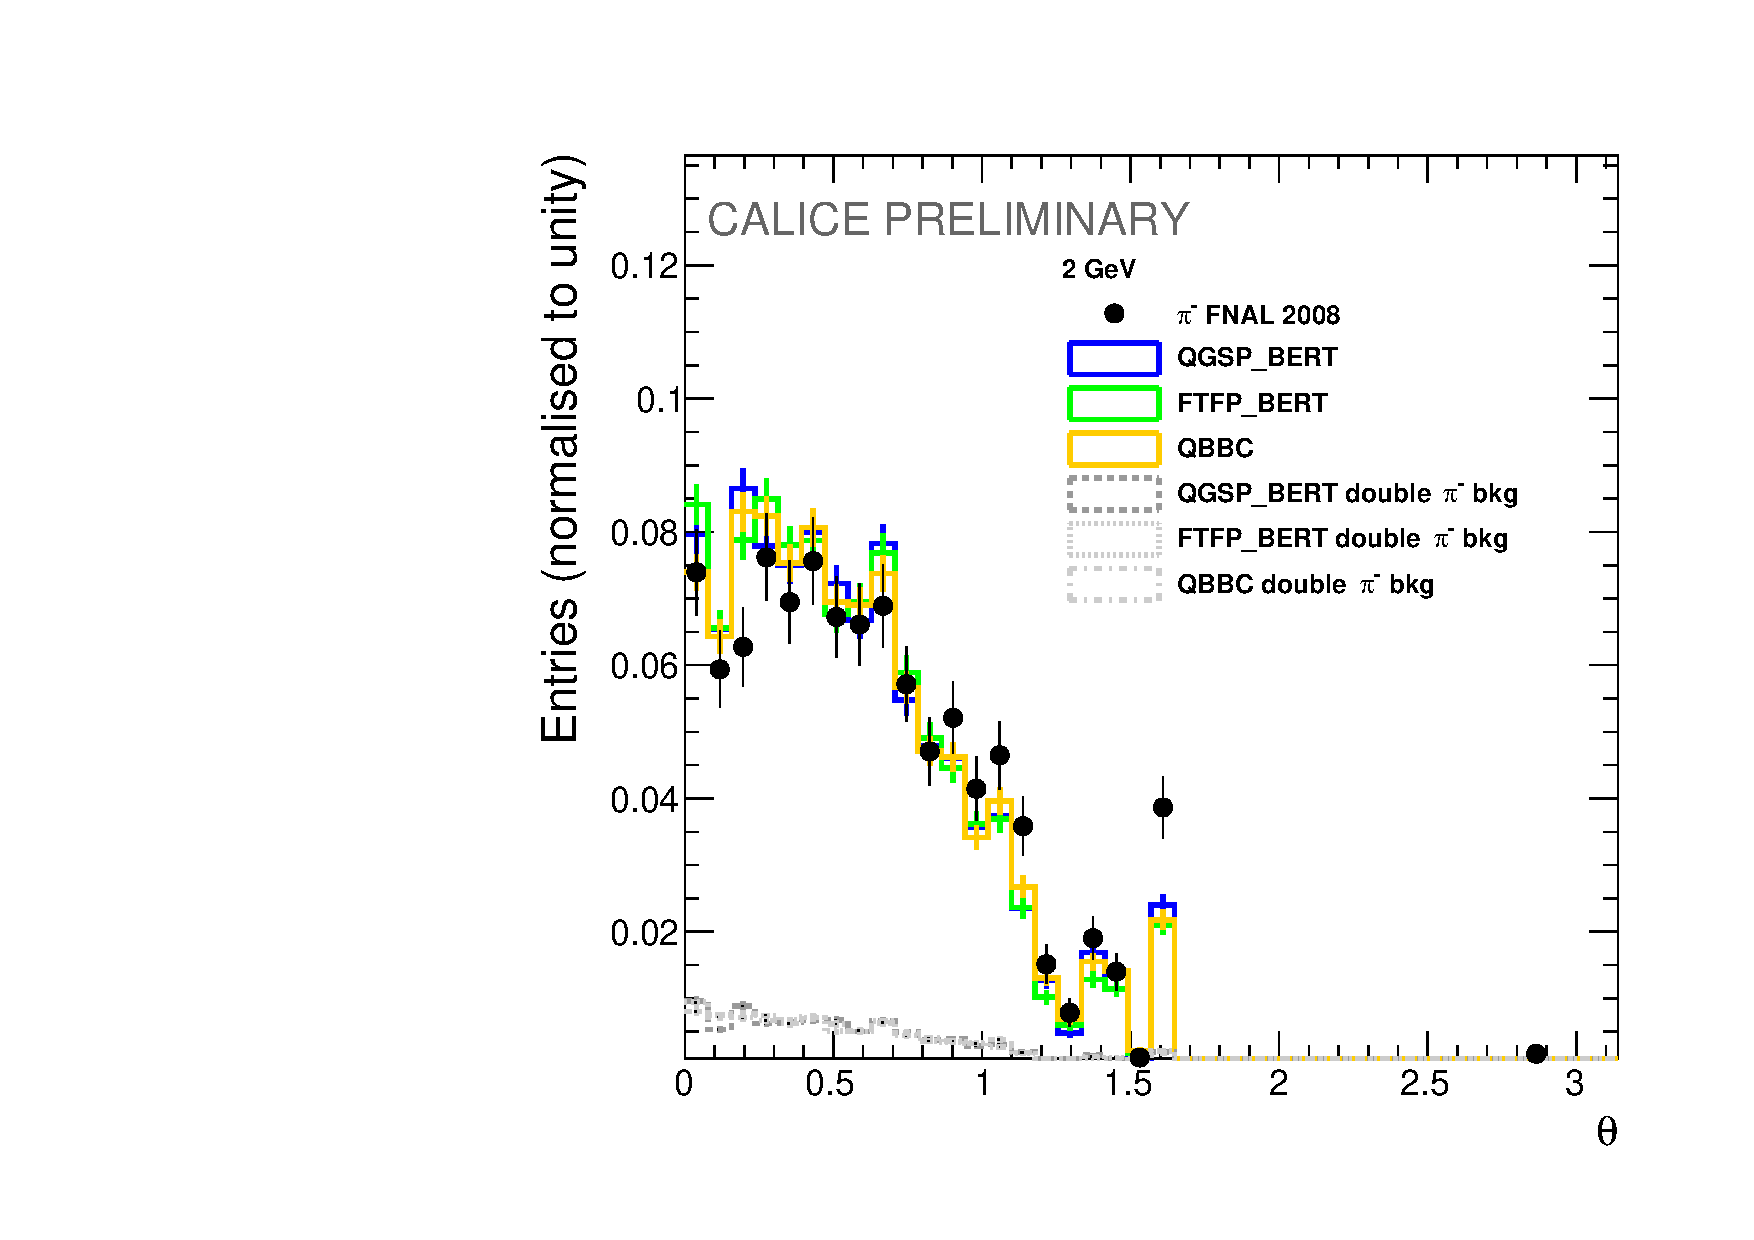
\includegraphics[width=.90\linewidth]{ECAL/plots/theta-2.pdf}
		\caption{\label{fig:theta2} }
	\end{subfigure}% 
	\begin{subfigure}{0.5\textwidth}
		\centering
		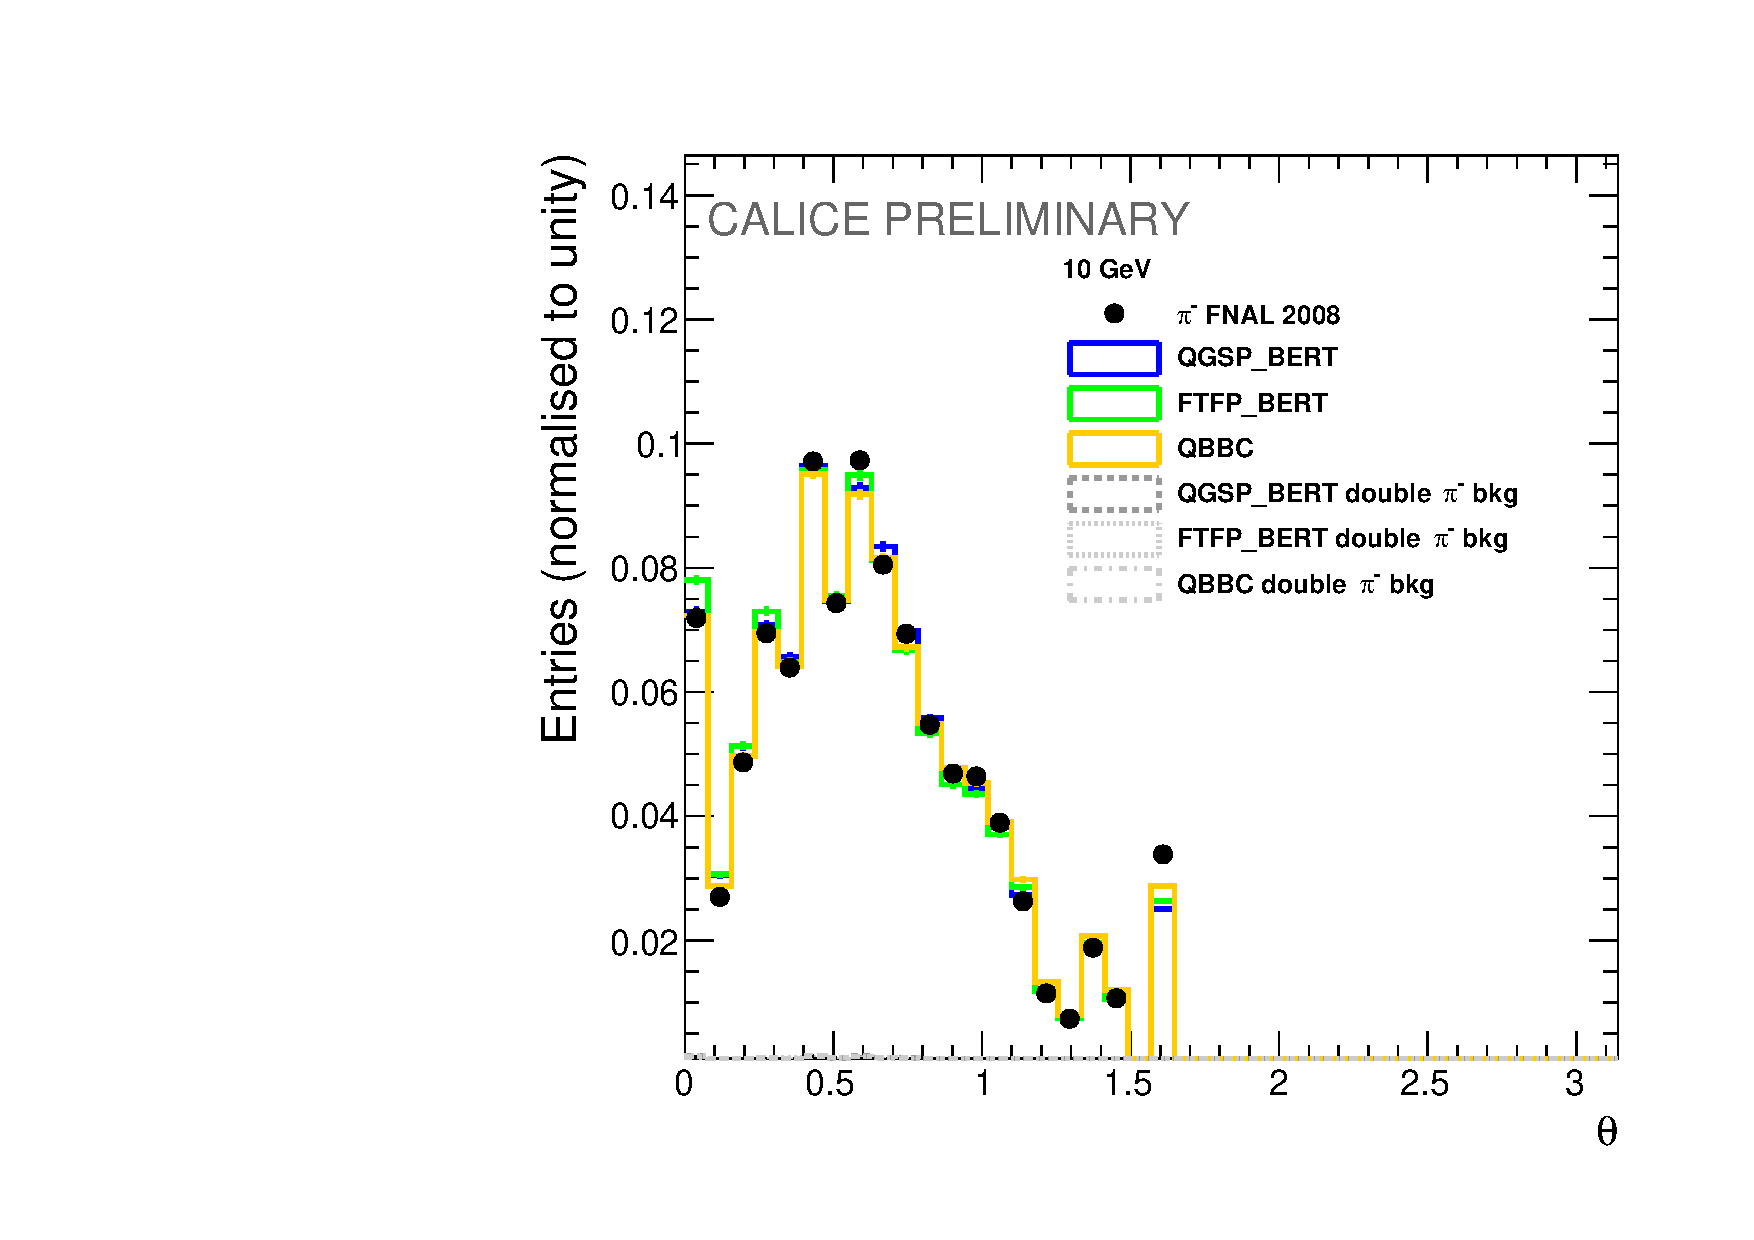
\includegraphics[width=.90\linewidth]{ECAL/plots/theta-10.pdf}
		\caption{\label{fig:theta10} }
	\end{subfigure}
	\caption{\label{fig:thetaexample} \sl Comparison of the polar angle $\theta$ of secondary tracks found between data and Monte Carlo simulations for two {\sc Geant}4 physics lists for energies of the primary particle of 2 (a) and 10 (b) GeV, respectively. Events without a detected interaction region according to Sec.~\ref{sec:iazone} are discarded. Error bars represent statistical uncertainties only.}
\end{figure}

\begin{figure}
	\centering
	\begin{subfigure}{0.5\textwidth}
		\centering
		\includegraphics[width=.90\linewidth]{ECAL/plots/phi-2.pdf}
		\caption{\label{fig:phi2} }
	\end{subfigure}% 
	\begin{subfigure}{0.5\textwidth}
		\centering
		\includegraphics[width=.90\linewidth]{ECAL/plots/phi-10.pdf}
		\caption{\label{fig:phi10} }
	\end{subfigure}
	\caption{\label{fig:phiexample} \sl Comparison of the azimuthal angle $\phi$ of secondary tracks between data and Monte Carlo simulations for two {\sc Geant}4 physics lists for 2 (a) and 10 (b) GeV beam energies. Events without a detected interaction region according to Sec.~\ref{sec:iazone} are discarded. Error bars represent statistical uncertainties only.}
\end{figure}

\begin{figure}
	\centering
	\begin{subfigure}{0.5\textwidth}
		\centering
		\includegraphics[width=.90\linewidth]{ECAL/plots/theta-graph.pdf}
		\caption{\label{fig:thetagraph}}
	\end{subfigure}% 
	\begin{subfigure}{0.5\textwidth}
		\centering
		\includegraphics[width=.90\linewidth]{ECAL/plots/delta-theta-graph.pdf}
		\caption{\label{fig:dthetagraph} }
	\end{subfigure}
	\caption{\label{fig:fullthetagraph} \sl Mean polar angle $\left<\theta\right>$ of secondary tracks for $\varepsilon = 0.03$  (a) and the corresponding sensitivity according to Eq.~\ref{eq:sens} of $\left<\theta\right>$ on the \ep\,(b) for data and Monte Carlo simulations for two {\sc Geant}4 physics lists as a function of beam energy. The sensitivity, see Eq.~\ref{eq:sens}, is estimated by the mean difference in $\theta$ for $\varepsilon = 0.04$ and $\varepsilon_{nom} = 0.02$. Events without a detected interaction region according to Sec.~\ref{sec:iazone} are discarded. Error bars represent statistical errors and the error band the systematic error from the correction for double $\pi$ events.}
\end{figure}
A further discussion on the relationship between the \ep ,  the polar angle $\theta$ and the track length $l$ can be found in Appendix~\ref{app:b}.

%||||||||||||||||||||MPV energy deposition|||||||||||||||||||||
\subsection{Energy deposition by secondary tracks}

%The developed \tfa\ can select tracks from MIP-like particles in the \ecal\ that have no electron contamination.
%The secondary tracks in hadronic cascades should have the same mean energy deposition for any initial particle energy.
At energies relevant for this study, the secondaries that create sizeable tracks, cross the detector volume as minimal ionising particles. 
%This motivates to investigate whether the secondary tracks can be used for an in-situ MIP calibration of the \ecal. 
This fact may be exploited for an in-situ calibration of the detector or at least for a monitoring of the response of individual detector regions. For this purpose the following additional selection cuts are applied: 
\begin{itemize}
	\item The events are required to have more than one track and an interaction region to suppress soft inelastic scattering interaction for lower energies;
	\item The reconstructed tracks should have a length $l\geq 8$ and $l / N_{hits} > 0.9$ to select long pencil-like tracks;
	\item the reconstructed tracks should have an polar angle $\theta < 0.3$ to reduce the angular dependence of the energy depositions.
\end{itemize}

The energy deposition by secondary tracks $E_{dep}^t$ using data for 2 and 10\,GeV beam energy is displayed in Fig. \ref{fig:calib}. Both distributions peak at around 1\,MIP as expected for straight MIP like tracks. Overlaid is a fit of the convolution of a Landau and a Gaussian that approximates well the measured distribution. However, as can be already inferred from Fig.~\ref{fig:calib2}, the tighter selection criteria reduce considerably the statistics at 2\,GeV. As a consequence, the uncertainty on the fit is large for the 2\,GeV sample. The data at 2\,GeV are thus discarded in the following.

Figure \ref{fig:calibrationgraph} presents the dependence of the most probable value (MPV) of the energy deposition in secondary tracks on beam energy. 
It can be seen that the detector response is uniform within 1-2\% over the energy range of the primary particles in data and that also the energy deposition by the tracks is reproduced by the Monte Carlo simulations within 1-2\%.  

\begin{figure}
	\centering
	\begin{subfigure}{0.5\textwidth}
		\centering
		\includegraphics[width=.90\linewidth]{ECAL/plots/calibrationfit-2.pdf}
		\caption{\label{fig:calib2} }
	\end{subfigure}% 
	\begin{subfigure}{0.5\textwidth}
		\centering
		\includegraphics[width=.90\linewidth]{ECAL/plots/calibrationfit-10.pdf}
		\caption{\label{fig:calib10} }
	\end{subfigure}
	\caption{\label{fig:calib} \sl Histograms of the energy deposition in secondary tracks for the data with 2 (a) and 10 (b) GeV beam energies. The spectra are fitted by the convolution of a Landau and a Gaussian. Events without a detected interaction region according to Sec.~\ref{sec:iazone} are discarded. Error bars represent statistical uncertainties only.}
\end{figure}

\begin{figure}
	\centering
	\includegraphics[width=0.5\textwidth]{ECAL/plots/calibrationfit-graph.pdf}
	\caption{\label{fig:calibrationgraph} \sl MPV of the Landau fit to the $E_{dep}^t$ distributions of the pencil-like secondary tracks as a function of the beam energy for $\pi^-$ data and three Monte Carlo samples. The MPV point the of 2\,GeV data sample is excluded because of the small statistics left after selection. Events without a detected interaction region  according to Sec.~\ref{sec:iazone} are discarded.  Error bars represent the statistical fit uncertainty.}
\end{figure}

This result is not trivial. It shows that the algorithm has indeed selected MIP-like secondary tracks since the MIP scale is expected to be independent of the underlying physics lists and the detector response should be largely independent of the energy of the primary particle. 

%-------------------------------------------------------------
%------------------------SUMMARY------------------------------
%-------------------------------------------------------------
\section{Summary and outlook}

This study reveals the outstanding potential of the CALICE \ecalp\ to obtain a detailed picture of the interactions of hadrons with matter. 
This note describes basic ideas and the application of a new simple \tfa\ for the \ecal. This algorithm allows for the reconstruction of tracks produced by secondary particles created in the interaction of hadrons with the absorber material, and hence to study the interaction region of hadronic showers in the \ecal. The \tfa\ produces a new set of differential observables, based on reconstructed tracks of secondary particles and the interaction region of the hadronic cascades. The results are stable w.r.t. small variations of the main parameter of the \tfa.

Data recorded in test beams at FNAL in 2008 with pions as primary particles with energies between 2 and 10\,GeV are compared with predictions by the physics lists \qgsp\, \ftfp\ and \qbbc as contained in {\sc Geant4} version 10.01. The accuracy with which the simulation describes the data varies with the beam energy and the chosen physics observable. In most of the cases data and Monte Carlo agree within 10\% without revealing a clear preference for one of the chosen physics lists. In this context it is worthwhile to remind that the interaction region is systematically 10\% wider than it is the case for the Monte Carlo simulation.

The largest source of discrepancy between data and Monte Carlo is the energy and radius of the interaction region. The measured energy deposition in the interaction region is up to 20\% higher than predicted by the Monte Carlo simulation.
The distributions of the number of secondary tracks and the number of hits per track for data are well described by the used physics lists. The polar angles of reconstructed tracks in the Monte Carlo simulation agree with data within 8\% on average and the distribution azimuthal angles is well reproduced by the Monte Carlo simulations even in view of the non trivial detector geometry.

%The new observables are sensitive to the different hadronic models implemented in the physics lists. 
%The mean polar angle of detected tracks as a function of the beam energy has a visible transition between Fritiof and Bertini cascades in the \ftfp\ physics list, as well as between Bertini and LEP models in the \qgsp\ physics list. The same effects can be seen for other observables. 

With respect to a more general outlook future work should aim at transferring the insights about the interaction region and the secondaries emerging from it to the optimisation of Particle Flow Algorithms.

A tighter track selection leads to clean MIP-like tracks. The detector response is stable to about 1-2\% over the tested energy range with an expected good agreement with Monte Carlo simulations. This observation can be exploited in the future as a starting point for a study on the possibility of an in-situ calibration or at least a regular monitoring of the detector by means of the selected tracks.  


%In conclusion, there is no preference for {\sc Geant4} physics lists as none of the two models, used in the analysis, describe the data in high detail. 
%-------------------------------------------------------------------
%-------------------------BIBLIOGRAPHY------------------------------
%-------------------------------------------------------------------
%\begin{thebibliography}{100} 
%\bibitem{bib:Calorimetry} J. C. Brient, H. Videau,\emph{ The calorimetry at the future $e^+e^-$ linear collider}, in: Proceedings of the APS / DPF / DPB Summer Study on the Future of Particle Physics (Snowmass 2001), 2001,arXiv:hep-ex/0202004v1.
%\bibitem{bib:ecal} The CALICE collaboration, \emph{Design and electronics commissioning of the physics prototype of a Si-W electromagnetic calorimeter for the International Linear Collider}, J. Instrum. 3 (2008) P08001, arXiv:0805.4833v1 [physics.ins-det]
%\bibitem{bib:Naomi} The CALICE Collaboration,  \emph{Testing Hadronic Interaction Models using a Highly Granular Silicon-Tungsten Calorimeter}, Nucl. Instrum. Meth. A Volume 794, Pages 240–254, arXiv:1411.7215v2 [physics.ins-det]
%\bibitem{bib:2010_CALICE_2} The CALICE Collaboration, C. Adloff, et al., \emph{Construction and Commissioning  of the CALICE Analog Hadron Calorimeter Prototype}, J. Instrum.~(5)  (2010) P05004, arXiv:1003.2662v1 [physics.ins-det].
%\bibitem{bib:2012_CALICE} The CALICE Collaboration, C. Adloff, et al., \emph{Construction and performance of a silicon photomultiplier/extruded scintillator tail-catcher and muon-tracker}, J. Instrum. (7) (2012) P04015, arXiv:1201.1653 [physics.ins-det].
%\bibitem{bib:G4pl} The {\sc Geant}4 Collaboration, \emph{Reference Physics Lists}, \url{http://Geant4.cern.ch/support/proc_mod_catalog/physics\_lists/referencePL.shtml}
%\bibitem{bib:HLi} \emph{Higgs Recoil Mass and Cross-Section Analysis at ILC And Calibration of the CALICE SiW ECAL Prototype}, Ph.D. thesis, Universit\'e Paris Sud   - Paris XI (2012).
%\bibitem{bib:2012_Doublet} P.Doublet, \emph{Hadrons dans un calorim\`etre \'electromagn\'etique   silicium-tungst\`ene hautement granulaire -- Production du quark top \'a   l'International Linear Collider}, Ph.D. thesis, Universit\'e Paris Sud   - Paris XI (2012).
%\end{thebibliography}

%\end{footnotesize}




\newpage\part{Heavy quark production at the ILC}\label{PARTIII}

\section{Heavy quark phenomenology and New Physics}
\label{sec:Phenomenology}
The mass of the top quark is comparable with the electroweak vacuum expectation value and it is much higher than weak boson masses. 
This fact makes the top quark a subject of many New Physics theories. 
The measurements of the bottom quark properties, the partner of the top quark, have revealed a deviation with the \sm\ prediction. 
Many \bsm\ theories predict modifications of the electroweak production of the heavy quarks pairs compared to the \sm\ expectations. 
Therefore, precise measurements of heavy quark couplings are required for indirect searches of new particles and discrimination between various theories. 

This section concentrates on the electroweak production of the top and bottom quarks pairs.%, corresponding observables, heavy quark production at linear colliders and possible influence of New Physics.
Other sources of the electroweak production as e.g. single top are not covered in the thesis. 

%the higgs is tightly connected to the top quark via coupling that is proportional to the top mass
%The bottom quark is in the same doublet as top

%%%%%%%%%%%%%%%%%%%%%%%%%%%%%%%%%%%%%%%%%%%%%%
%%%%%%%%%%%%%%%%%%%%%%%%%%%%%%%%%%%%%%%%%%%%%%
%%%%%%%%%%%%%%%%%%%%%%%%%%%%%%%%%%%%%%%%%%%%%%
\subsection{Description of the heavy quark production}
%First, one needs to define the most convenient parametrization of coupling or form factors of interest, and then express the observable quantities in terms of defined form factors. 
Electroweak production of the fermion pairs proceeds through the $f\bar{f}X$ vertex, where $X$ represents neutral vector bosons, photon or $Z^0$ boson.  The current at the $f\bar{f}X$ vertex can be expressed via form factors $F$ as 
\begin{equation}
\Gamma^{f\bar{f}X}_\mu (k^2,q,\bar{q}) = ie\{ \gamma_\mu (F^X_{1V}(k^2) + \gamma^5 F^X_{1A}(k^2)) - \frac{\sigma_{\mu\nu}(q-\bar{q})^\nu}{2m_f}(iF^X_{2V}(k^2) + \gamma^5 F^X_{2A}(k^2)) \},
\end{equation}
where $k^2= (q+\bar{q})^2$ is the four momentum squared of the exchanged vector boson, $q$ and $\bar{q}$ are the four vectors of the fermion $f$ and antifermion $\bar{f}$ and $m_f$ is the fermion mass. Further, $\gamma_\mu$ and $\gamma_5$ are the Dirac matrices, and $\sigma_{\mu\nu} = i/2(\gamma_\mu\gamma_\nu - \gamma_\nu\gamma_\mu)$.

The \sm\ values of the form factors are the following:
\begin{equation}
F^{f\gamma}_{1V} = Q^{f}, \ F^{f\gamma}_{1A} = 0, \ F^{fZ}_{1V} = \frac{I^f - 2Q^f\sin^2\theta_W}{2\cos\theta_W\sin\theta_W}, \ F^{fZ}_{1A} = - \frac{I^f}{2\cos\theta_W\sin\theta_W},
\label{formula:SMformFactors_3}
\end{equation}
and all $F_2$ factor are zero. In the Eq.~\ref{formula:SMformFactors_3} $I^f$ is the weak isospin number, $I^t = 1/2$ for top and $I^b = -1/2$ for bottom quark and $Q^f$ is the electric charge, $Q^t = 2/3$ and $Q^b = -1/3$.

%The form factors are related to fermion couplings with left and right-handed helicity to $Z^0$ boson:
The following definition of the left-handed and right handed $Z^0b\bar{b}$ couplings is used throughout the thesis: 
\begin{equation}
%g_L^Z = (F_{1V}^Z - F_{1A}^Z), \  g_R^Z = F_{1V}^Z + F_{1A}^Z, 
g_L^Z = I^f - Q^f\sin^2\theta_W, \  g_R^Z = -Q^f\sin^2\theta_W, 
\label{formula:EWcouplings_3}
\end{equation}
%the same relations are applied to the corresponding photon couplings $g^\gamma_L$.
%At the tree level, the \sm\ differential cross for the production
%of a fermion $f$ pair in $e^+e^-\to f\bar{f}$ at center-of-mass energy $\sqrt[]{s}$ can be written as

In case of the polarized beams, the fermion form factors can be expressed in terms of the helicity of the initial electrons~\cite{bib:Schmidt}:
\begin{eqnarray}
\mathcal{F}^L_{ij} = - F^\gamma_{ij} +  \frac{-1/2 + \sin^2\theta_W}{\cos\theta_W\sin\theta_W}\frac{s}{s-M^2_Z+i\Gamma_ZM_Z}F^Z_{ij},\\
\mathcal{F}^R_{ij} = - F^\gamma_{ij} +  \frac{\sin^2\theta_W}{\cos\theta_W\sin\theta_W}\frac{s}{s-M^2_Z+i\Gamma_ZM_Z}F^Z_{ij}    
\label{formula:PolFF_3}
\end{eqnarray}

where $i=1,2$ and $j=V,A$, $M_Z$ and $\Gamma_Z$ are the $Z^0$ boson mass and width, respectively.

The key expression for the studies is the differential cross section of $f\bar{f}$ production for electron beam polarization $I=L,R$, expressed via the defined form factors:

\begin{multline}
% \frac{\pi\alpha^2 N_c\beta}{s}
\label{formula:DiffSigma_3}
\frac{d\sigma^I}{d\cos\theta} = \frac{3}{4} \mathcal{A} N_c \beta[ (1+\cos^2\theta) [(\mF_{1V}+\mF_{2V})^2+(\beta \mF_{1A})^2] - \\-4 \cos\theta (\mF_{1V}+\mF_{2V})\beta \mF_{1A} +\\+ \sin^2\theta [\gamma ^{-2} (\mF_{1V} +\gamma^2 \mF_{2V})^2] ]
\end{multline}
where $\mathcal{A} = 4\pi\alpha^2/3s$ with $\alpha$ as the electromagnetic running coupling, $N_c$ is the number of quark colors, $\beta$ and $\gamma$ are the velocity and the Lorentz factor of the produced fermion, respectively. 

One can derive from (\ref{formula:DiffSigma_3}) the total cross section, a common observable, which can be expressed as
%2\frac{4\pi\alpha^2}{3s}N_c\beta
\begin{equation}
\label{formula:TotalSigma_3}
\sigma^I_{total} = 2\mathcal{A}N_c\beta[(1+\frac{1}{2}\gamma^{-2})(\mathcal{F}^I_{1V})^2 + (\beta\mathcal{F}^I_{1A})^2+3\mathcal{F}^I_{1V}\mathcal{F}^I_{2V}+(1+\frac{1}{2}\gamma^{2})(\mathcal{F}^I_{2V})^2],
\end{equation}
The term $\beta \mF_{1A}$ describes the reduced sensitivity to the axial form factors near the $f\bar{f}$ production threshold. 


Another typical observable is the forward-backward asymmetry, which is defined as
\begin{equation}
A_{FB}^I = \mp \mathcal{A} N_c \frac{3\beta\mathcal{F}^I_{1A}(\mathcal{F}^I_{1V} + \mathcal{F}^I_{2V})}{\sigma^I_{total}}.
\label{formula:AfbForm_3}
\end{equation}

This observable has a large sensitivity to the axial form factor $\mathcal{F}^I_{1A}$, therefore it is crucial to measure $A_{fb}^I$ precisely to reduce uncertainty on the corresponding form factors.
%%%%%%%%%%%%%%%%%%%%%%%%%%%%%%%%%%%%%%%%%%%%%%
%%%%%%%%%%%%%%%%%%%%%%%%%%%%%%%%%%%%%%%%%%%%%%
%%%%%%%%%%%%%%%%%%%%%%%%%%%%%%%%%%%%%%%%%%%%%%
\subsection{Observables of interest}
The conventional approach used to estimate the couplings or form factors of the fermion $f$ to the vector bosons $\gamma /Z^0$ is to measure the total cross section $\sigma_I$ and forward-backward asymmetry \afb.

The total cross section is measured knowing the number of accepted events $N$, selection efficiency $\epsilon$ and integrated luminosity $\mathcal{L}_{total}$
\begin{equation}
\sigma_{total} = \frac{N}{\epsilon \mathcal{L}_{total}}.
\label{formula:Xsection_3}
\end{equation}
The corresponding uncertainty on the cross section is determined by the knowledge of the machine luminosity and the statistics of the signal: 
\begin{equation}
	(\frac{\delta \sigma_{total}}{\sigma_{total}})^2 = (\frac{\delta N}{N})^2 + (\frac{\delta \mathcal{L}_{total}}{\mathcal{L}_{total}})^2.
\end{equation}

The beams of the $e^+e^-$ colliders, like ILC, will not be fully polarized, therefore one should take into account the electron beam polarization degree $\mathcal{P}$ and positron polarization degree $\mathcal{P}'$. 
The expression for the total cross section is then
\begin{equation}
\label{formula:RealSigma_3}
\sigma_{\mathcal{P}\mathcal{P}'} = \frac{1}{4}[(1-\mathcal{P}\mathcal{P}')(\sigma_{LR}+\sigma_{RL} ) + (\mathcal{P} - \mathcal{P}')(\sigma_{RL} - \sigma_{LR})],
\end{equation}
where the indices $L$ and $R$ indicate full polarization of the incoming electron and positron beams of left-handed or right-handed helicity, respectively.

The forward-backward asymmetry is an observable, which counts the difference between the number of events in the forward region and backward regions:
\begin{equation}
A_{FB} = \frac{\sigma(cos\theta > 0) - \sigma(cos\theta < 0)}{\sigma(cos\theta > 0) + \sigma(cos\theta < 0)}.
\end{equation}
The statistical uncertainty on the \afb\ as for a simple counting experiment is given by 
\begin{equation}
\delta A_{FB} = \sqrt{\frac{1-A_{FB}^2}{N}},
\end{equation}
where $N$ is the number of reconstructed events. 

%For the proper \afb\ measurement,  it is crucial to measure the charge of the quarks with a high purity. 
%single top
%Another source of top quark production at linear colliders is the single top process. %which is shown in Fig. \ref{fig:singletop_3}. 
%This process allows top quark production at 250\,GeV center-of-mass energy, but the study of the single top production is not included in the thesis. 
%%%%%%%%%%%%%%%%%%%%%%%%%%%%%%%%%%%%%%%%%%%%%%%%%%%%%%%%%%%%%%%%
%%%%%%%%%%%%%%%%%%%%%%%%%%%%%%%%%%%%%%%%%%%%%%%%%%%%%%%%%%%%%%%%
%%%%%%%%%%%%%%%%%%%%%%%%%%%%%%%%%%%%%%%%%%%%%%%%%%%%%%%%%%%%%%%%
\subsubsection{New Physics influence}
%The heavy quarks and the Higgs boson are often subject of \bsm\ deviations.
%For example, supersymmetric extensions of the \sm\ predict different set of Higgs couplings to the up type and down type quarks. 

The extradimentional extensions of the \sm\ like Randall-Sundrum models~\cite{Randall:1999ee} are able to provide an explanation to the fermion mass hierarchy, and have additional weak boson excitations. 
These theories have additional weak bosons $Z'$ or $W'$ with a mixing to the \sm\ bosons, which can modify the electroweak couplings of the heavy quarks. 
The possible compositness of heavy quarks can also leave an imprint on the their electroweak couplings.
These models can have different impact on the left-handed or right handed couplings on the electroweak couplings of the heavy quarks. 

\begin{figure}[h]
	{\centering
		\includegraphics[clip, trim=4cm 7cm 2cm 10cm, width=0.95\textwidth]{ILD/graphics/plot.pdf}
		\caption{\sl Predictions of several models that incorporate Randall-Sundrum (RS) models and/or compositeness or Little Higgs models on the deviations of the left- and right-handed couplings of the $t$~quark to the $Z^0$ boson. The ellipse in the frame in the upper right corner indicates the precision that can be expected for the ILC running at a center-of-mass energy of $\sqrt[]{s} = 500\,GeV$ after having accumulated ${\mathcal L}=500\,fb^{-1}$ of integrated luminosity shared equally between the beam polarizations $P(e^-),\,P(e^+) =\pm0.8,\mp0.3$. The original version of this figure can be found in~\cite{bib:ILCTOP}.}
		\label{fig:DeviationsTop}
	}
\end{figure}

The relative deviations of the left-handed and right-handed couplings of the top quark are predicted by various BSM theories are shown in Fig.~\ref{fig:DeviationsTop}.
A precise measurement of the top quark couplings allows for identification of the particular BSM theory.
  
%Concerning the \bbbar\ channel, experiments with polarized beams have an advantage of sign flip detection of the right-handed coupling $g_R^Z$, which can be produced by the Randall-Sundrum models with $Z^0$-$Z'$ mixing~\cite{bib:RSTOP}.
%
%Many \bsm\ models predict deviations on the heavy quark couplings to the Higgs and weak bosons.


%\begin{figure}[H]
  \centering
\setlength{\unitlength}{1.5mm}
%\setlength{\unitlength}{\textwidth} 

\begin{picture}(150,90)
\linethickness{0.3mm}
%\begin{center}
%compose x axis
  \put(9,33){\line(0,1){2}}
  \put(5,34){\line(1,0){8}}  
  \put(15,34){...} 
  \put(21,34){\vector(1,0){60}} 
  \put(82,33){\Large{$\delta g^Z_R / g^Z_R$}}
  \multiput(31,33)(10,0){5}{\line(0,1){2}} 
  \put(6.5,31){\footnotesize{-330\%}} 
  \put(29,31){\footnotesize{-20\%}} 
  \put(39,31){\footnotesize{-10\%}}
  \put(60,31){\footnotesize{10\%}}
  \put(70,31){\footnotesize{20\%}}
%compose y-axis
  \put(51,4){\vector(0,1){60}} 
  \put(45,66){\Large{$\delta g^Z_L / g^Z_L$}}
  \multiput(50,14)(0,10){5}{\line(1,0){2}} 
  \put(45,13.5){\footnotesize{-20\%}} 
  \put(45,23.5){\footnotesize{-10\%}} 
  \put(45.5,43.5){\footnotesize{10\%}} 
  \put(45.5,53.5){\footnotesize{20\%}}
%Add models
  \put(51,34){\color{red}\circle*{2}} 
  \put(53,36){\color{red}SM}
  \put(51,24){\color{britishracinggreen}\circle*{1.5}}
  \put(53,23){\color{britishracinggreen}Light top partners~\cite{Grojean:2013qca}}
  \put(41,24){\color{britishracinggreen}\circle*{1.5}} 
  \put(21,26){\color{britishracinggreen} Light top partners}
 \put(21,23){\color{britishracinggreen} Alternative 1~\cite{bib:panico-priv}}
  \put(76,59){\color{britishracinggreen}\circle*{1.5}} 
  \put(56,61.5){\color{britishracinggreen} Light top partners Alternative 2~\cite{bib:panico-priv}}
  %\put(53,23){\color{green}Composite Higgs with SO(5)/SO(4)}%~\cite{Grojean:2013qca}}
   \put(51,19){\color{cyan}\circle*{1.5}} 
   \put(53,18){\color{cyan}Little Higgs~\cite{Berger:2005ht}}
  \put(51,14){\color{gray}\circle*{1.5}} 
  \put(53,13){\color{gray}RS with Custodial SU(2)~\cite{Carena:2006bn}}
  \put(51,9){\color{orange}\circle*{1.5}} 
  \put(53,8){\color{orange}Composite Top~\cite{Pomarol:2008bh}}
  \put(31,14){\color{magenta}\circle*{1.5}} 
  \put(20,16){\color{magenta}5D Emergent~\cite{Cui:2010ds}}
  \put(56,29){\color{camel}\circle*{1.5}} 
  \put(58,28){\color{camel}4D Composite Higgs Models~\cite{Barducci:2015aoa}}
  \put(9,34){\color{blue}\circle*{1.5}} 
  \put(1,36){\color{blue}RS with Z-Z' Mixing~\cite{Djouadi:2006rk}}
%make a box to put the ILC precision into
\multiput(56,40)(30,0){2}{\line(0,1){12}} 
\multiput(56,40)(0,12){2}{\line(1,0){30}}
\put(61,47){\large{ILC Precision}}
%embed the covariance ellipse
\color{red}
% Ellipse:  u = 71.0  v = 43.0  a = 2.45336  b = 0.631947  phi = 16.9866 Grad
\qbezier(73.3463, 43.7167)(73.2699, 43.9671)(72.5286, 43.9342)
\qbezier(72.5286, 43.9342)(71.7873, 43.9013)(70.8154, 43.6044)
\qbezier(70.8154, 43.6044)(69.8435, 43.3075)(69.2103, 42.9205)
\qbezier(69.2103, 42.9205)(68.5772, 42.5336)(68.6537, 42.2833)
\qbezier(68.6537, 42.2833)(68.7301, 42.0329)(69.4714, 42.0658)
\qbezier(69.4714, 42.0658)(70.2127, 42.0987)(71.1846, 42.3956)
\qbezier(71.1846, 42.3956)(72.1565, 42.6925)(72.7897, 43.0795)
\qbezier(72.7897, 43.0795)(73.4228, 43.4664)(73.3463, 43.7167)
\end{picture}





\caption{\sl Predictions of several models that incorporate Randall-Sundrum (RS) models and/or compositeness or Little Higgs models on the deviations of the left- and right-handed couplings of the $t$~quark to the $Z^0$ boson. The ellipse in the frame in the upper right corner indicates the precision that can be expected for the ILC running at a centre-of-mass energy of $\sqrt[]{s} = 500\,GeV$ after having accumulated ${\mathcal L}=500\,fb^{-1}$ of integrated luminosity shared equally between the beam polarisations $P(e^-),\,P(e^+) =\pm0.8,\mp0.3$. The original version of this figure can be found in~\cite{bib:ILCTOP}.}
\label{fig:models-rp}
\end{figure}
%Supersymmetric models  -  have different set of Higgs couplings to the up and down type quarks.
%%%%%%%%%%%%%%%%%%%%%%%%%%%%%%%%%%%%%%%%%%%%%%%%%%%%%%%%%%%%%%%%
%%%%%%%%%%%%%%%%%%%%%%%%%%%%%%%%%%%%%%%%%%%%%%%%%%%%%%%%%%%%%%%%
%%%%%%%%%%%%%%%%%%%%%%%%%%%%%%%%%%%%%%%%%%%%%%%%%%%%%%%%%%%%%%%%
\subsection{Status of the measurements and simulation studies}
%mass measurements

\subsubsection{Measurements at LEP and SLC}
%The electron-positron colliders have a large production cross section of $e^+e^- \to q\bar{q}$ process mediated by $Z^0$ boson or a virtual photon.
The total cross sections of various \sm\ processes for the $e^+e^-$ machines are shown in Fig.~\ref{fig:LCcrosssection}.

The circular LEP~I and the linear SLC colliders operated at the $Z^0$ pole, where the $e^+e^-$ cross section is maximal as seen from Fig.~\ref{fig:LCcrosssection}.
The measurements resulted in extremely precise b-quark fraction $R_b$ and the b-quark forward-backward asymmetry $A_{FB}^b$ measurements. 
The measured $R_b$ value, which is the ratio of b-quark cross section over total hadronic cross section, has full compatibility with the \sm\ prediction. 
On the other hand, the measured b-quark forward-backward asymmetry $A_{FB}^b$, dominated by the LEP~I precision, has 2.5\,$\sigma$ deviation with the recent electroweak fit predictions~\cite{bib:AfbSMFit}.
%The measurement of the $A_{FB}^b$ value at the SLC have 27\% higher uncertainty than the LEP results~\cite{bib:SLC}.

\begin{figure}[h]
	{\centering
		\includegraphics[clip, trim=0.5cm 5cm 0.5cm 7cm, width=0.95\textwidth]{ILD/graphics/epem_sm-hepph.pdf}
		\caption{\sl Tree-level cross sections of major \sm\ processes at linear colliders as function of center-of-mass energy assuming no polarization of the initial state~\cite{bib:Han}.}
		\label{fig:LCcrosssection}
	}
\end{figure}


The measurements outside $Z^0$ pole were carried out by the LEP~II programme, which collected the most integrated luminosity at around 190\,GeV energy, at the $W^\pm$-pair production threshold. 
The measured $A_{FB}^b$ at this center-of-mass energy agrees within 2\,$\sigma$ with the tree level \sm\ prediction.

The polarized initial state at the SLC allowed to introduce the left-right asymmetry $A(SLD)$.
This observable measures the difference between the left-handed and the right-handed initial state polarization cross sections. The measured value of the left-right asymmetry for leptons $A_l(SLD)$ has 2\,$\sigma$ deviation from the \sm\ prediction~\cite{bib:AfbSMFit}. The computed values of $\sin^2\theta_W$ using $A_{FB}^b$ from LEP and $A_l(SLD)$ differ significantly.

The precise determination of the $Zb\bar{b}$ vertex at LEP~I and SLC experiments allowed to put constraints on the top quark and Higgs boson masses.
The LEP measurement allowed to predict the top quark mass in the region of 133\,GeV $ < m_t < $ 190\,GeV and the Higgs boson mass  10\,GeV $< m_H <$ 440\,GeV~\cite{bib:LEPTOP}, which were later confirmed by the TeVatron and the LHC experiments. 
%$A_{fb}^b(\sqrt[]{s} = 190.7\,\text{GeV})=0.51\pm0.058$
%Unfortunately, the beam energies of LEP~II and SLC was not high enough to produce single top or top quark pairs, therefore, the precise determination of the top electroweak couplings is left for the future electron-positron machines.

\subsubsection{LHC and TeVatron measurements}
The composite nature of colliding particles at the hadron colliders priviledges the production of the top quark pairs through the strong interaction via high cross section $gg\to t\bar{t}$ or $q\bar{q}\to t\bar{t}$ processes.
Therefore, the hadron machines can measure the top mass as the cross section parameter with a high precision. 

The TeVatron has a high production rate of the single top-quark via $q\bar{q}' \to W^\pm \to t\bar{b}$ process. %at a higher rate than proton-proton machines. 
This process involve $tbW$ vertex and therefore, its total cross section depends on the weak couplings of the top quark. 
The measurement of the single top cross section at TeVatron is found to be consistent with the \sm\ predictions~\cite{bib:TeVstop} with about 16\% uncertainty.

The measurements of the forward-backward asymmetry at TeVatron~\cite{bib:TeVAfb} and the charge asymmetry at the LHC~\cite{Naranjo:2017etb} of the strong $t\bar{t}$ production are consistent with the \sm\ expectations. 

To measure the electroweak couplings of the top quark at the LHC, the associate production of top quark pair with $Z^0$ or $W^\pm$ bosons is required, which has a lower cross section, than the \ttbar\ production process.
Study of the $t\bar{t}Z^0$ process has been done at the LHC experiments using Run I data with $\sqrt{s} = 8$\,TeV. It shows compatible rates of the signal process with the \sm, but more statistics is required to measure the cross section precisely~\cite{bib:CMSttz2014}. The cross section fit results for the $t\bar{t}Z^0$ and $t\bar{t}W^\pm$ processes are shown in Fig~\ref{fig:LCHTopTopZ_3}.
Including the Run~II data of the LHC with a higher center-of-mass energy will significantly improve $t\bar{t}Z^0$ measurement.
%Main channel of the top quark production is gluons
\begin{figure}[h]
	{\centering
		\includegraphics[ width=0.55\textwidth]{ILD/graphics/fit_2d.pdf}
		\caption{\sl The result of the two-dimensional best fit for $t\bar{t}W^\pm$ and $t\bar{t}Z^0$ cross sections (cross symbol) is shown along with its 68 and 95\% confidence level contours by the CMS experiment. The result of this fit is superimposed with the separate $t\bar{t}W^\pm$ and $t\bar{t}Z^0$ cross section measurements, and the corresponding 1 standard deviation (1\,$\sigma$) bands, obtained from the dilepton, and the trilepton/four-lepton channels, respectively. The figure also shows the predictions from theory and the corresponding uncertainties.~\cite{bib:CMSttz2014}.}
		\label{fig:LCHTopTopZ_3}
	}
\end{figure}
%ttZ cross section measurements

The study of the b-quark electroweak couplings is very limited at hadron colliders.
The possible $Z^0b\bar{b}$ associate production study at the LHC can provide only the cross section magnitude value, which has been measured at LEP~I to have no deviation from the \sm\ prediction. 
Top quark have never been studied at the $e^+e^-$ colliders, benefiting from a direct electroweak production and a high signal over background ratio.
Hence, precise measurements of the heavy quark electroweak couplings are left for future $e^+e^-$ machines.




%2.5s tension by LEP in bbar asymmetry
\subsubsection{Future linear colliders}

The acceleration technologies available today allow for the construction and the running of a linear electron-positron collider at center-of-mass energies well above top pair production threshold. The clean environment of the linear colliders allows detection and reconstruction of all \sm\ decay modes of the top quark: fully leptonic, semileptonic and fully hadronic decays. 



As can be seen from expression of the differential cross section~(\ref{formula:DiffSigma_3}), the sensitivity to axial form factors is proportional to the fermion velocity $\beta$, therefore, the higher beam energies, like 500\,GeV stage at the ILC are preferred for a study of electroweak top quark couplings. 
The b-quark coupling analysis can be done at all center-of-mass energies, scheduled at the ILC project.


%Matrix element method fully leptonic
%Such assets of the future $e^+e^-$ colliders as high signal-to-noise ratio and high-granularity of the detectors allow to use Matrix Element Method to compute the form factors from a kinematical fit of the top pair decay products. 
%This method can be applied at the ILC for fully leptonic decay of the top quark pair. 

The first top quark electroweak coupling analysis at the ILC was published in Ref.~\cite{bib:ILCTOP}, where the uncertainties on the form factors (\ref{formula:SMformFactors_3}) and the couplings (\ref{formula:EWcouplings_3}) were estimated using the ILD environment.


The semileptonic top decays were used in~\cite{bib:ILCTOP}, where  a lepton from leptonic top quark decay $t\to b l \bar{\nu_l}$ provides the charge information, and jets from hadronic top quark decays $t \to b q \bar{q}'$ are used for top polar angle reconstruction. 
It was found that, an accidental assignment of the hadronic $W^\pm$ jets to the b-jet from leptonic top quark decays can happen. This mistake 
amounts to flip the value of $\cos\theta_{top}$ into $-\cos\theta_{top}$, which lead to a large deviation from the generated polar angle distribution, as shown in Fig.~\ref{fig:ILCTOPAFB_a_3}.
This effect is called an event migration problem.
Only the left-handed electron beam distribution is affected due to the $W^\pm$ boson kinematics, as explained in~\cite{bib:ILCTOP}. 
%CLIC

The study of the electroweak top couplings at CLIC was done at $\sqrt{s} = 380$\,GeV~\cite{bib:Garcia}. This study confirms the event migration effect.


There are two possible ways to remedy the migration effect problem - by doing a kinematical cut on $\chi^2_{top}$, which is a measure of hadronic top reconstruction quality, or by finding a correct combination of lepton charge with the b-quark charge. 
The main advantage of the combination with the b-quark charge is that this method do not require precise knowledge of the top quark decay kinematics, as it is needed for the $\chi^2_{top}$ cut method. 
The reconstructed top polar angle distribution for semileptonic decay of the top quark pair is shown in Fig.~\ref{fig:ILCTOPAFB}, where one sees the $W^\pm$ lepton migration effect caused by the $W^\pm$ kinematics and the resolution of the problem by the kinematical cut on $\chi^2_{top}$ in Fig.~\ref{fig:ILCTOPAFB_b_3}.


\begin{figure}[H]
	\centering
	\begin{subfigure}{0.5\textwidth}
		\includegraphics[clip, trim=0.9cm 0cm 0.9cm 0cm,width=0.99\textwidth]{ILD/graphics/EPS_AFB_nocut.pdf}
		\caption{\label{fig:ILCTOPAFB_a_3} }
	\end{subfigure}% 
	\begin{subfigure}{0.5\textwidth}
		\centering
		\includegraphics[clip, trim=0.9cm 0cm 0.9cm 0cm,width=0.99\textwidth]{ILD/graphics/AFB_wbkg_chi2cut.pdf}
		\caption{\label{fig:ILCTOPAFB_b_3} }
	\end{subfigure}
	\caption{\sl Reconstructed top quark polar angle before (a) and after $\chi^2_{top}$ cut (b) distributions compared with the prediction by the event generator for two configurations of the beam polarizations~\cite{bib:ILCTOP}. }
	
	\label{fig:ILCTOPAFB}
\end{figure}

The first attempt to use the quark charge technique in fully hadronic \ttbar\ decays was done by~\cite{amjad:tel-00949818}, but it required large simulation-dependent corrections. 
Hence, one needs to investigate the reasons of inefficiency and impurity of the quark charge measurement in the ILD environment and propose a method to fix the problems. 



The development of the b-quark charge measurement will increase the statistics for semileptonic \ttbar\ channel,  open access to the fully hadronic \ttbar\ decay channels without any Monte-Carlo corrections and, moreover, it will allow a study of electroweak coupling of the bottom quark, which have never been done using the ILC environment. 


%Study of precision of ILC on top couplings were made by Amjad et al. using semileptonic decays. 
%Central problem: migration effect of the lepton from W. 
%B charge was first used as a way to remove migration effect by Jeremy for semileptonic channel.  and Amjad for hadronic one. 
%Development of quark charge measurement technique willl increase the statistics for semileptonic channel, and open hadronic top decays. 
%The quark charge measurement is the only way to study the bbbar process.  

%%%%%%%%%%%%%%%%%%%%%%%%%%%%%%%%%%%%%%%%%%%%%%%%
%%%%%%%%%%%%%%%%%%%%%%%%%%%%%%%%%%%%%%%%%%%%%%%%
%%%%%%%%%%%%%%%%%%%%%%%%%%%%%%%%%%%%%%%%%%%%%%%%

\section{B-quark charge reconstruction}
\label{sec:JetChargeReconstruction}
An information about the bottom quark charge is useful for all \sm\ processes, where b-jets appear as decay products. 
In this thesis it is used for quark polar angle reconstruction of $e^+e^-\to t\bar{t}$ and $e^+e^- \to b\bar{b}$ processes. 
The polar angle spectrum is used to determine the quark couplings. 
This requires a high purity and a high efficiency of the b-quark charge reconstruction, which is an ultimate challenge for every reconstruction algorithm and all subdetectors of the experiment. 

One of the main goals of this thesis is to develop a method of the b-quark charge measurement with high purity and efficiency using the full simulation of the ILD experiment. 
To do so, first, it is necessary to measure the performance of the standard reconstruction algorithm and find sources of charge impurities, and then develop an algorithm to improve it. 


%%%%%%%%%%%%%%%%%%%%%%%%%%%%%%%%%%%%%%%%%%%%%%%%%%%%%%%%%%%
%%%%%%%%%%%%%%%%%%%%%%%%%%%%%%%%%%%%%%%%%%%%%%%%%%%%%%%%%%%
%%%%%%%%%%%%%%%%%%%%%%%%%%%%%%%%%%%%%%%%%%%%%%%%%%%%%%%%%%%
\subsection{Setup of the study}

All studies in this and the next chapters are done using full simulation of the baseline ILD experiment. 
The b-quark charge measurement study uses $e^+e^- \to b\bar{b}$ at $\sqrt[]{s} = 250$\,GeV and the semileptonic decay mode of the $e^+e^- \to t\bar{t}$ at $\sqrt[]{s} = 500$\,GeV processes generated using {\sc whizard}~1.95 event generator. 
The hadronization of the quarks and gluons is done by the {\sc pythia}~6.205 event generator.
The distributions of the b-hadron momentum, generated by {\sc pythia} for the 250\,GeV $b\bar{b}$ and the 500\,GeV $t\bar{t}$ pairs are shown in Fig.~\ref{fig:GenHadronMomentum_3}. 
The distributions have different peak energies, bur the energy range is the same. Further analysis shows, that this difference has small impact on the performance of the quark charge reconstruction.
\begin{figure}[h]
	{\centering
		\includegraphics[width=0.45\textwidth]{ILD/plots/gen-hadron-momentum.pdf}
		\caption{\sl Generated b-hadron momentum by {\sc pythia} for \bbbar\ and \ttbar\ pair production processes signal processes.}
		\label{fig:GenHadronMomentum_3}
	}
\end{figure}

The $B^0-\bar{B}^0$ oscillations are enabled in the {\sc pythia} simulation. 
The ILD detector layout, the interaction of particles with the detector material and the detector response are simulated by the {\sc mokka} framework, that provides the geometry interface to the \geant\ toolkit. 

All reconstruction algorithms, along with the {\sc mokka} framework are part of the {\sc ilcsoft} software toolkit.
The modular structure of the {\sc ilcsoft} allows for independent execution of each reconstruction algorithm. 

%The ILD collaboration defines the order of the standard reconstruction chain, which is applied to all studies done using the full simulation of the ILD experiment. 

The most relevant standard reconstruction algorithms of the {\sc ilcsoft} for the b-quark charge measurement are described below:
\begin{itemize}
\item The MarlinTrk package organizes the hits, created by particles in the ILD trackers into reconstructed tracks. The track parametrization in described in~\cite{bib:LCIOtrack}. 
\item The PandoraPFA package is responsible for the clusterization of the calorimeter hits and creation of the Particle Flow Objects. The track covariance matrix is used to compute the covariance matrix of the reconstructed particle momentum; 
\item The primary and secondary vertex reconstruction is done by the Linear Collider Flavour Identification Plus or LCFI+ algorithm~\cite{bib:LCFI}. 
\end{itemize}
Each reconstructed track by the MarlinTrk algorithm has 5 parameters and the corresponding associated covariance matrix with 15 parameters; The most important for the thesis are the impact parameters $d_0$ and $z_0$, which are the transverse and longitudinal distance between the point of the closest approach to the reference point $(0,0)$, respectively. The corresponding uncertainties are $\sigma_{d_0}$ and $\sigma_{z_0}$, respectively.

The jet clustering algorithms can be configured and launched according to the analysis requirements. 
The flavor-tagging at the ILD experiment will serve to separate out jets from bottom and charm quarks from the light quark or gluon jets, the corresponding separation variables are called b- and c-tagging, respectively. 
The flavor-tagging algorithm within the LCFI+ package provides  b- and c-tagging information for each reconstructed jet.


%%%%%%%%%%%%%%%%%%%%%%%%%%%%%%%%%%%%%%%%%%%%%%%%%%%%%%%%%
%%%%%%%%%%%%%%%%%%%%%%%%%%%%%%%%%%%%%%%%%%%%%%%%%%%%%%%%%
%%%%%%%%%%%%%%%%%%%%%%%%%%%%%%%%%%%%%%%%%%%%%%%%%%%%%%%%%
\subsection{Bottom quark topology}

The charge of the b-quark can be derived from the properties of the b-hadron and its decay products. 
%Therefore, one needs to know precisely the properties of the underlying hadrons. 


The b-quark hadronization modes are displayed in Table~\ref{table:bhadrons}.
        \begin{table}[H]
        \begin{center}
        \begin{tabular}{l c c }
        \hline
        			& Branching ratio & $c\tau$ \\
        \hline
            \Bm\ meson & $40.4 \pm 0.6 $\% & 450\,$\mu$m \\
            \Bz\ meson & $40.4 \pm 0.6 $\% & 455.4\,$\mu$m  \\

            \Bzs\ meson & $10.3 \pm 0.5 $\% & 453.3\,$\mu$m   \\
         \hline
            b-baryon & $8.9 \pm 1.3 $\% & $\approx$ 447\,$\mu$m  \\

        \hline
        \end{tabular}
        \end{center}
        \caption{\sl Hadronization modes of the b-quark~\cite{bib:PDG}. }
        \label{table:bhadrons}
        \end{table}

These branching fractions are approximate and may have a dependency on the initial and final state kinematic and production environment~\cite{bib:PDG}.
However, the presence of the \Bzs\ meson increase the number of the neutral hadronization modes, which will cause additional complications for the charge measurement. 
The illustration of the b-quark hadronization and common decay modes are given in Fig.~\ref{fig:Bmodes_3}.
\begin{figure}[h]
	{\centering
		\includegraphics[width=0.55\textwidth]{ILD/plots/b-modes}
		\caption{\sl The illustration of the b-quark hadronisation and decay modes with the corresponiding decay rates in percent. Modes in the red circle are not tracked by the TruthVertexFinder.}
		\label{fig:Bmodes_3}
	}
\end{figure}

%b-hadron decays, typically, the charged pions, kaons, leptons or protons, 
Due to the Lorentz boost given by the initial b-quark energy, the b-hadron can travel several millimeters before its decay. Due to this flight distance, the charged particles from the b-hadron decays will have an offset with respect to the primary interaction point, which is the main signature of the b-quark jets. 

%Therefore we expect two vertices
The B meson have $D^0$ or $D^\pm$ meson decay modes of about 80\% decay rate, mediated by the weak interaction. The charmed $D$ mesons have a mean lifetime of $c\tau \approx 120 - 300$\,$\mu$m, which gives a possibility to the charmed mesons to travel away from the initial B meson decay vertex. 
Hence, one expects to detect two vertices from one b-jet in most of the cases: the secondary, which corresponds to the b-hadron decay, and the tertiary vertex created by the c-hadron decays. 

The $K^\pm$ mesons from B meson decays are the end products of the $b\to c\to s$ decay chain mediated by the weak interaction. 
The $K^\pm$ mesons have a long lifetime with $c\tau = 3.7$\,m and a high mass of 493.6\,MeV comparing with another long-lived charged particles from the B meson decays, like pions or leptons. 
Hence, it is possible to identify kaons by their energy deposition in the detector, which depend on particle mass. 
In the generator, about 87\% of b-hadrons are set to have correlated $K^\pm$ charge in the generator, which makes the $K^\pm$ charge a reliable indication of the initial b-quark charge. The kaon charge was used to determine the b-quark charge at the SLC~\cite{Falciai:1996jv} and the LEP experiments~\cite{Abreu:1999ui}.
On contrary, the b-baryons tend to produce protons, which have an opposite sign of charge to the initial b-quark charge.

%%%%%%%%%%%%%%%%%%%%%%%%%%%%%%%%%%%%%%%%%%%%%%%%%%%%%%%
%%%%%%%%%%%%%%%%%%%%%%%%%%%%%%%%%%%%%%%%%%%%%%%%%%%%%%%
%%%%%%%%%%%%%%%%%%%%%%%%%%%%%%%%%%%%%%%%%%%%%%%%%%%%%%%
\subsubsection{Generated vertices}
The output of the event generators is a list of generated particles with parent-child relations. 
The TruthVertexFinder algorithm was developed to find the generated vertices.%, and included into the {\sc ilcsoft} distribution. 
This algorithm detects the generated b-hadrons, finds the related charged particles, which can leave reconstructable tracks and organizes them into the generated secondary or tertiary vertices.



\begin{figure}
	\centering
	\begin{subfigure}{0.5\textwidth}
		\includegraphics[width=0.95\textwidth]{ILD/plots/gen-b-vtx.pdf}
		\caption{\label{fig:GenVtx_a_3} }
	\end{subfigure}% 
	\begin{subfigure}{0.5\textwidth}
		\centering
		\includegraphics[width=0.95\textwidth]{ILD/plots/gen-c-vtx.pdf}
		\caption{\label{fig:GenVtx_b_3} }
	\end{subfigure}
	\caption{\sl Distributions of the b-vertex charge multiplicity~(a) and c-vertex charge multiplicity~(b). }
	\label{fig:GenVtx_3}
\end{figure}

%Generator distributions


%The b-hadrons can be identified by measuring the charged tracks, which have an offset from primary interaction point caused by the b-hadron lifetime.
%B*
The high-energy b-quarks can hadronize into excited states of the b-hadrons, which can decay into their ground state by emitting charged or neutral pion. 
The charged pion from the excited b-hadrons can distort the charge multiplicity distributions, leading to an incorrect comparison with the reconstructed vertices. Therefore, the TruthVertexFinder selects only ground state hadrons within a decay chain. 

The TruthVertexFinder finds vertices from b-hadron decays and subsequent c-hadron decay vertices. The distributions of generated b- and c-vertices are displayed in Fig.~\ref{fig:GenVtx_3}. 
The c-vertex multiplicity distribution is consistent with~\cite{bib:PDG}. 
One notices that about 31\% of the b-vertices and 13\% of the c-vertices decay into one generated prong, which poses a challenge to the vertexing algorithms. This problem will be addressed in Sec.~\ref{sec:MisVertices}.

\begin{figure}
	{\centering
		\includegraphics[width=0.75\textwidth]{ILD/plots/offset-graph.pdf}
		\caption{\sl Illustration of particle offset variable $\epsilon$, where $\vec{p}$ is a vector of a given particle momentum, $B$ is a flight distance of a b-hadron, $\vec{IP}$ is a primary vertex position, $\vec{t}_0$ is a point of the closest approach of a given particle. 
		}
		\label{fig:OffsetPic_3}
	}
\end{figure}

The particle offset or the impact parameter is the minimal distance between the particle trajectory and the interaction point, as illustrated in Fig.~\ref{fig:OffsetPic_3}.
This is the main observable used by the vertex reconstruction algorithms. 
The offset distributions of the generated b-vertex and c-vertex prongs are shown in Fig.~\ref{fig:GenVtxOffset_3}.
Majority of the generated prongs have large offsets above the ILD impact parameter resolution of 5\,$\mu$m. 
As can be seen from Fig.~\ref{fig:GenVtxOffset_3}, the c-vertex prong offsets are larger than b-vertex prong offsets, because of the additional distance traveled by c-hadron from the b-hadron decay point. 

\begin{figure}
\centering
\begin{subfigure}{0.5\textwidth}
    \includegraphics[width=0.95\textwidth]{ILD/plots/gen-bvtx-offsets.pdf}
\caption{\label{fig:GenVtxOffset_a_3} }
\end{subfigure}% 
  \begin{subfigure}{0.5\textwidth}
\centering
    \includegraphics[width=0.95\textwidth]{ILD/plots/gen-cvtx-offsets.pdf}
\caption{\label{fig:GenVtxOffset_b_3} }
\end{subfigure}
    \caption{\sl Distributions of the b-vertex (a) and c-vertex prong offsets~(b). }
    \label{fig:GenVtxOffset_3}
\end{figure}

The distributions of the total B-hadron charge multiplicity and the b-jet multiplicity are displayed in Fig.~\ref{fig:GenHadronParams_3}. The mean b-jet multiplicity is almost three times higher than the mean B-hadron multiplicity, which makes the vertex reconstruction a non trivial task. 
The imbalance between the odd and even number of multiplicities shown in Fig.~\ref{fig:GenHadronParams_a_3} is caused by the presence of the \Bzs\ hadronization modes.

Regarding the similarity of the distributions for two processes shown in Figures~\ref{fig:GenVtx_3}, \ref{fig:GenHadronParams_3} and \ref{fig:GenVtxOffset_3}, the performance of a vertexing algorithm should be identical for the same energy and the direction of the b-hadron decays.


\begin{figure}
\centering
\begin{subfigure}{0.5\textwidth}
    \includegraphics[width=0.95\textwidth]{ILD/plots/gen-hadron-multiplicity.pdf}
\caption{\label{fig:GenHadronParams_a_3} }
\end{subfigure}% 
  \begin{subfigure}{0.5\textwidth}
\centering
    \includegraphics[width=0.95\textwidth]{ILD/plots/jet-multi.pdf}
\caption{\label{fig:GenHadronParams_b_3} }
\end{subfigure}
    \caption{\sl Left: Distribution of the b-hadron charge multiplicity. The odd multiplicities correspond to the charged hadrons and the even multiplicities correspond to the neutral hadron decays. Right: Distribution of the reconsructed b-jet multiplicities for two processes. }
    \label{fig:GenHadronParams_3}
\end{figure}


%The design of the ILD vertex detector is optimized to have the best offset resolution 

%%%%%%%%%%%%%%%%%%%%%%%%%%%%%%%%%%%%%%%%%%%%%%%%%%%%%%%%%
%%%%%%%%%%%%%%%%%%%%%%%%%%%%%%%%%%%%%%%%%%%%%%%%%%%%%%%%%
%%%%%%%%%%%%%%%%%%%%%%%%%%%%%%%%%%%%%%%%%%%%%%%%%%%%%%%%%

\subsection{Standard vertex reconstruction in the ILD}
The LCFI+ package finds the secondary and tertiary vertices and tags the b- and c-jets using the charged particles among the Particle Flow objects.
It has several stages of the vertex reconstruction and flavor-tagging, which are implemented in the following algorithms:
\begin{itemize}
\item PrimaryVertexFinder finds the position of the primary interaction point and the corresponding charged particles;
\item BuildUpVertex forms the reconstructed vertex candidates, which can have two or more associated charged particles, referred in the text as reconstructed prongs;
\item JetVertexRefiner finds vertices with only one prong using the reconstructed vertex candidates and it organizes the vertex candidates into maximum two reconstructed vertices per jet.
\item FlavorTag algorithm calculates b-tag and c-tag values for a jet, using the finalized jet vertices from the JetVertexRefiner. The b-tag and c-tag values are the measure of b- and c-likeness of a jet, respectively, both observables have values from 0 to 1. Performance of the flavor-tagging algorithm is shown in Fig.~\ref{fig:LCFIplus_3}.
\end{itemize}

\begin{figure}
	{\centering
		\includegraphics[width=0.45\textwidth]{ILD/graphics/btag-cbg.eps}
		\caption{\sl The tagging efficiency is shown for b-jets with the mis-identification	fraction evaluated using c-jets. Solid lines correspond to the case of 2-jet events at $\sqrt{s} = 91$\,GeV. Dashed lines correspond to the case of 6-jet events at	$\sqrt{s} = 500$\,GeV. Dotted lines correspond to the case of 6-jet events at $\sqrt{s} = 1000$\,GeV~\cite{bib:LCFI}.
		}
		\label{fig:LCFIplus_3}
	}
\end{figure}
In this section, only the standard reconstruction chain is used to study the b-quark charge measurement. 


%\subsubsection{Baseline quark charge reconstruction}
The b-quark charge is computed as a sum of the reconstructed particles charges, associated to the reconstructed vertices, which belong to a given jet. 
Therefore, the vertexing algorithm should correctly associate all secondary or tertiary vertex particles to have a correct b-quark charge measurement. 
The correctly reconstructed b-quark charge should have the same  charge as the generated b-hadron. 
%Regarding the b-hadron multiplicity, shown in Fig.~\ref{fig:GenHadronParams_a_3}, and the b-jet multiplicity in Fig.~\ref{fig:GenHadronParams_b_3} this task is not trivial. 

%%%%%%%%%%%%%%%%%%%%%%%%%%%%%%%%%%%%%%%%%%%%%%%%%%%%
%%%%%%%%%%%%%%%%%%%%%%%%%%%%%%%%%%%%%%%%%%%%%%%%%%%%
%%%%%%%%%%%%%%%%%%%%%%%%%%%%%%%%%%%%%%%%%%%%%%%%%%%%
\subsubsection{B-quark charge purity: State of the art}
The charge purity $P_B$ is defined as the number of correctly reconstructed b-quark charges $N_{correct}$ divided by the total number of jets $N_{total}$:
\begin{equation}
	\label{formula:Purity_3}
	P_B = \frac{N_{correct}}{N_{total}}.
\end{equation} 
The previous studies carried out for the fully hadronic $t\bar{t}$ decays~\cite{Amjad:2014tha} have shown that the total b-quark charge purity $P_B$ is about 60\%.
The total b-quark charge for the considered $b\bar{b}$ process  is $P_B(b\bar{b}) = 66\%$ and for semileptonic decay of the  $t\bar{t}$ pair is $P_B(t\bar{t}) = 64\%$. 
The small difference between these values is caused mostly by the difference in the generated momentum  distributions displayed in Fig.~\ref{fig:GenHadronMomentum_3} and by the difference in the jets environments.

Using the output of the TruthVertexFinder, one compares the generated vertices with the corresponding reconstructed vertices, detected by the LCFI+ algorithms. 
Figure~\ref{fig:Table_3} shows the comparison of the number of the generated prongs $N_{gen}$ with the number of the reconstructed prongs $N_{rec}$ on the jet-per-jet basis. 
The row with $N_{rec} = 0$ are the jets, which have no associated reconstructed vertices, will cause the efficiency decrease in the b-quark charge measurement, however, they have no influence on the method purity.
The jets with reconstructed vertices have the following statistics:
\begin{itemize}
\item Only 49\% of these jets are perfectly reconstructed and have $N_{rec}=N_{gen}$;
\item The 46\% of the jets have lost one or more prongs from the reconstructed vertices having $N_{rec}<N_{gen}$;
\item The rest 5\% are the jets with vertices, contaminated by particles with non b-hadron origin and have $N_{rec}>N_{gen}$.
\end{itemize}

\begin{figure}
{\centering
    \includegraphics[width=0.55\textwidth]{ILD/plots/rec-gen-table.pdf}
    \caption{\sl Comparison of the number of reconstructed tracks $N_{gen}$ to the number of generated tracks $N_{rec}$ for a given b-jet. The number of entries is color-coded for each cell. The diagonal has 49\% of all entries and it contains the jets, which have the correctly reconstructed vertices. The b-jets below diagonal have vertices with one or more particles missed by reconstruction. The row $N_{rec} = 0$ corresponds to the b-jets with no reconstructed vertices. %Right: Same comparison, but after a cut on the b-tag$> 0.8$ and a cut on the b-hadron momentum more than 20\,GeV. The diagonal contains 55\% of the jets after the cuts.
    }
    \label{fig:Table_3}
  }
\end{figure}

The jets with $N_{rec}=N_{gen}$ have the charge purity of more than 97\%, while all other jets have an almost random reconstructed b-quark charge with the corresponding charge purity about 35\%.
The fraction of entries below the diagonal in Fig.~\ref{fig:Table_3} is small, comparing to the fraction of events above the diagonal. 
Hence, the purity reduction is mainly caused by the jets, which have lost the prongs from their reconstructed vertices. 
%The application of cuts, for example on jet b-tag$>0.8$ and reconstructed b-hadron momentum $|p_{had}| > 20$\,GeV, increases the fraction of correctly reconstructed jets up to 55\%, however with an efficiency penalty of 17\%.
%The cuts on the b-tag value are necessary to reject background processes and will be adjusted to archieve the best background suppression. 


Therefore, there is a possibility to develop a recovery algorithm, which can add the missing prongs to the reconstructed vertices.
%, with a slight increase of the number of jets with contaminated vertices. 
But first, one needs to study the reasons behind the missing prongs and analyze the possibility to recover them. 

%%%%%%%%%%%%%%%%%%%%%%%%%%%%%%%%%%%%%%%%%%%%%%%%%%%%
%%%%%%%%%%%%%%%%%%%%%%%%%%%%%%%%%%%%%%%%%%%%%%%%%%%%
%%%%%%%%%%%%%%%%%%%%%%%%%%%%%%%%%%%%%%%%%%%%%%%%%%%%
\subsubsection{Missing vertices}
\label{sec:MisVertices}
The vertex reconstruction algorithm may fail if the generated b-hadron properties, like number of generated prongs, b-hadron momentum or polar angle, are in the poor acceptance of the detector. 
The non-reconstructed vertices contain approximately 22\% of all generated b-hadron prongs. 
The b-hadron vertices with generated low momentum prongs or low offset prongs have higher chances to be missed by the reconstruction algorithms. 
The distributions of the average prong offset and momentum for reconstructed vertices and missed vertices are shown in Fig.~\ref{fig:RecMissedParams_3}. 
One concludes, that the reconstruction algorithms start to lose their efficiency at below 4\,GeV average prong momentum and below 0.5\,mm average prong offset. 


The polar angle distributions of the missing vertices is displayed in Fig.~\ref{fig:MissedCos_3}. 
One summarizes the reasons for missing vertices as following: 
\begin{itemize}
\item Neutral decay vertex - the vertex cannot be reconstructed if it has no generated prongs;
\item Low energy of the generated b-hadron causes a short flight distance, small offsets or low momentum of the generated prongs, which makes it difficult to separate out the b-hadron prongs from the other particles in a b-jet;
\item A one prong decay vertex can be lost if there was no other vertices reconstructed in a given b-jet;
\item Most of the b-hadrons, produced in the forward region, or outside the barrel VXD acceptance $|\cos\theta_{vtx}| > 0.95$, are not reconstructed, which is due to a low precision on the impact parameters of the reconstructed prongs. 
\end{itemize}

\begin{figure}
	\centering
	\begin{subfigure}{0.5\textwidth}
		\includegraphics[width=0.95\textwidth]{ILD/plots/rec-missed-p-vtx.pdf}
		\caption{\label{fig:RecMissedParams_a_3} }
	\end{subfigure}% 
	\begin{subfigure}{0.5\textwidth}
		\centering
		\includegraphics[width=0.95\textwidth]{ILD/plots/rec-missed-s-vtx.pdf}
		\caption{\label{fig:RecMissedParams_b_3} }
	\end{subfigure}
	\caption{\sl Distributions of the average prong momentum~(a) and offset (b) of the missed and reconstructed vertices. }
	\label{fig:RecMissedParams_3}
\end{figure}

\begin{figure}
	{\centering
		\includegraphics[clip, trim=10.cm 0cm 0.cm 0cm, width=0.55\textwidth]{ILD/plots/missed-cos-vtx.pdf}
		\caption{\sl Polar angle distribution of the missed vertices subdivided into different categories. This is a stacked histogram. The low momentum or low offset category are the missing vertices, which have the average prong momentum below  4\,GeV or below 0.5\,mm average prong offset.
		}
		\label{fig:MissedCos_3}
	}
\end{figure}
%An attempt was made to reduce the vertexing inefficiency in the forward region

The missing vertices are difficult to recover, however they have essentially no impact on the b-quark charge purity, therefore the further studies are focused on the missing prongs of the reconstructed vertices.
%%%%%%%%%%%%%%%%%%%%%%%%%%%%%%%%%%%%%%%%%%%%%%%%%%%%
%%%%%%%%%%%%%%%%%%%%%%%%%%%%%%%%%%%%%%%%%%%%%%%%%%%%
%%%%%%%%%%%%%%%%%%%%%%%%%%%%%%%%%%%%%%%%%%%%%%%%%%%%
\subsubsection{Missing prongs from the reconstructed vertices}
\label{sec:MissingProngs}
%The quality of the vertex reconstruction strongly depends on all reconstruction algorithms as well as on various geometry aspects of the ILD experiment. 

%Using TruthVertexFinder information and truth links to the reconstructed particles, one can find, that the 
The missing reconstructed prongs are approximately 10.4\% of the total generated prongs for the standard vertex reconstruction. 
The reasons for the missing prongs can be summarized as follows:
\begin{itemize}
\item No tracking information - the MarlinTrk algorithms fails to reconstruct the track. This category is tiny - only 0.93\% of the generated prongs;
\item No associated hits in the VXD or FTD - the track segment from the Vertex Detector or Forward Tracking Disks was not connected to the long TPC track segment. These reconstructed particles have large uncertainties on the impact parameters, which makes them not suitable for vertexing algorithms. They constitute 2.\% of the generated prongs;
\item No reconstructed PFO - the PandoraPFA fails to create the PFO from a reconstructed track. These tracks are discarded by the LCFI+ algorithms - 3.2\%  of the generated prongs;
\item Low generated momentum or offset  - the reconstructed particle was produced with impact parameters below the detector resolution - 3.1\%  of the generated prongs;
\item Other reasons connected to vertex fitting problems - 1.7\% of the generated prongs.
\end{itemize}



\begin{figure}
\centering
\begin{subfigure}{0.5\textwidth}
    \includegraphics[width=0.95\textwidth]{ILD/plots/missed-tracks.pdf}
\caption{\label{fig:MissingTracks_cos_3} }
\end{subfigure}% 
  \begin{subfigure}{0.5\textwidth}
\centering
    \includegraphics[width=0.95\textwidth]{ILD/plots/missed-momentum.pdf}
\caption{\label{fig:MissingTracks_p_3} }
\end{subfigure}
    \caption{\sl Polar angle~(a) and momentum~(b) distributions of the missing prongs subdivided into different categories. This is a stacked histogram. The peak at $|\cos\theta| = 0 $ is caused by the gap between TPC endplates, the peak at  $|\cos\theta| \approx 0.8$ is caused by barrel-endcap transition in the \ecal\ and the rapid increase at $|\cos\theta| \approx 0.9$ is caused by the barrel-endcap transition in the VXD and FTD system. }
    \label{fig:MissingTracks_3}
\end{figure}

\begin{figure}
	{\centering
		\includegraphics[width=0.55\textwidth]{ILD/graphics/directions.pdf}
		\caption{\sl Illustration of the polar angle directions in ILD layout, where one has peaks in the missing prongs distribution. 
		}
		\label{fig:ILDDirection_3}
	}
\end{figure}

These categories of the missing prongs can be illustrated by the polar angle histogram, shown in Fig.~\ref{fig:MissingTracks_cos_3}, which also reveals the following problems connected to the ILD geometry, see Fig.~\ref{fig:ILDDirection_3}:
\begin{itemize}
\item Small peak at $|\cos\theta| = 0$ is caused by the TPC cathode gap. 
\item Large peak at $|\cos\theta| \approx 0.8$ is caused by the PandoraPFO, which fails to connect a well reconstructed track with an offset to a segmented cluster located in the calorimeter barrel-endcap transition. This problem is specific to the b-hadron tracks;
\item Increase at $|\cos\theta| \approx 0.9$ correspond to the end of the full 3 double layer VXD acceptance, resulting in an increase in the impact parameter uncertainties of the reconstructed tracks. %caused by a connection problem between the VXD track segments, which are in the acceptance region of the two double-sided VXD layers, and the FTD track segments.
\end{itemize}

The recoverable prongs are those, which were lost because of the reconstruction problems, like the problems with the PFO creation, and not by the limited detector acceptance.  

%%%%%%%%%%%%%%%%%%%%%%%%%%%%%%%%%%%%%%%%%%%
%%%%%%%%%%%%%%%%%%%%%%%%%%%%%%%%%%%%%%%%%%%
%%%%%%%%%%%%%%%%%%%%%%%%%%%%%%%%%%%%%%%%%%%
\subsection{Vertex charge recovery}
\label{sec:VtxRecovery}
The objective of the vertex recovery algorithm is to add accurately the missing prongs to the reconstructed vertices, without contamination by the particles with non b-hadron origin or the background particles. 

%The most important observable for any vertexing algorithm is the particle offset $\epsilon$.
%The uncertainty on the offset $\sigma$ for a given reconstructed charged particle can be computed as 
%\begin{equation}
%	\sigma = \sqrt[]{\sigma_{d_{0}}^2 + \sigma_{z_0}^2},
%%\end{equation}
% 


In this study we use the following definition of the offset significance:

\begin{equation}
	\epsilon/\sigma = |\frac{d_0}{\sigma_{d_0}}| + |\frac{z_0 }{ \sigma_{z_0}}|,
\end{equation}
where $\sigma_{d_{0}}$ and $\sigma_{z_0}$ are the covariance matrix elements, provided by the track reconstruction algorithms.
The offset significance value depends strongly on the momentum of the particle, its polar angle and number of assigned VXD or FTD hits . 

Typically, the b-hadron prongs are generated with large offsets (Fig.~\ref{fig:GenHadronParams_b_3}), but the reconstruction can miss a reconstructed prong if it has a small offset significance. 
Hence, one needs another spatial separation variable, combined with the offset significance $\epsilon/\sigma$. 

%Another separation variable can make use of the reconstructed vertex position and the reconstructed track candidate parameters. 

The particle trajectory bending because of magnetic field is negligible at the small distance scales, like the b-hadron flight distance in Fig.~\ref{fig:GenHadronParams_b_3}. 
Therefore, in this studies, the reconstructed track helix is approximated by the reconstructed vector of particle momentum. 

Suppose, one has a reconstructed secondary vertex in a position $\vec{s}_{vtx}$ and a prong candidate with a momentum $\vec{p}$ and a track reference point $\vec{t}_0$, which is computed from track parameters $d_0$ and $z_0$.
This study uses an angle $\alpha$, as a second separation variable, defined as an angle between the particle momentum $\vec{p}$ and the vector of difference between the vertex position $\vec{s}_{vtx}$ and the track reference point $\vec{t}$. The angle $\alpha$ is illustrated in Fig.~\ref{fig:VtxRecovery_3}.

\begin{figure}
{\centering
    \includegraphics[width=0.75\textwidth]{ILD/plots/recovery-graph.pdf}
    \caption{\sl Illustration of the chosen separation variables of the vertex charge recovery algorithm, where $\vec{p}$ is a vector of a given particle momentum, $B$ is a flight distance of a b-hadron, $\vec{IP}$ is a primary vertex position, $\vec{t}$ is a reference point of a given particle, defined in \cite{bib:LCIOtrack}, $\alpha$ is the angle between $\vec{p}$ and $\vec{s}_{vtx}$ and $\epsilon$ is an offset distance of the particle. %Right: Same comparison, but after a cut on the b-tag$> 0.8$ and a cut on the b-hadron momentum more than 20\,GeV. The diagonal contains 55\% of the jets after the cuts.
    }
    \label{fig:VtxRecovery_3}
  }
\end{figure}

An algorithm, called VertexChargeRecovery, was developed to increase the b-quark charge purity by adding the missing prongs to the reconstructed vertices.  For a given jet, which has at least one associated reconstructed vertex, the VertexChargeRecovery has the following procedure:

\begin{itemize}
\item Preparation of the prong candidates - the algorithm uses all charged particles within a given jet as prong candidates. To recover the prongs, which has no reconstructed PFO, the program iterates throughout all reconstructed tracks and reconstructs them as charged PFOs without an associated calorimeter cluster. These new Particle Flow particles are used only if they have no duplicates in the previously selected jet particles;
\item All prong candidates are compared to the reconstructed prongs to avoid duplicates;
\item The separation variables $\alpha$ and $\epsilon$ are calculated for each prong candidate and a given reconstructed vertex;
\item The selection condition is defined using the $\alpha$ and $\epsilon$ distributions for true b-hadron prongs and background particles, which are displayed in Fig.~\ref{fig:RecoveryPurity_3}, suggest the following cuts:
\begin{equation}
\epsilon/\sigma > 2 + 25\cdot\alpha\text{ and } \alpha < 0.08.
\end{equation}
The recovery algorithm might have a different behavior in simulation, than in the real experiment, therefore, one should use a data-driven charge purity measurements, described in Sec.~\ref{sec:ChargePurity}, to test and tune the recovery parameters.
\item The algorithm creates new reconstructed vertices with old and recovered reconstructed prongs and links them to a given jet.
\end{itemize}

\begin{figure}
	\centering
	\begin{subfigure}{0.33\textwidth}
		\includegraphics[clip, trim=0.1cm 0cm 13.8cm 0cm,width=0.99\textwidth]{ILD/plots/recovery-purity.pdf}
		\caption{\label{fig:RecoveryPurity_a_3} Missing particles}
	\end{subfigure}% 
	\begin{subfigure}{0.33\textwidth}
		\centering
		\includegraphics[clip, trim=6.78cm 0cm 7.1cm 0cm,width=0.99\textwidth]{ILD/plots/recovery-purity.pdf}
		\caption{\label{fig:RecoveryPurity_b_3} Background}
	\end{subfigure}
	\begin{subfigure}{0.33\textwidth}
		\centering
		\includegraphics[clip, trim=13.5cm 0cm 0.4cm 0.cm,width=0.99\textwidth]{ILD/plots/recovery-purity.pdf}
		\caption{\label{fig:RecoveryPurity_c_3} Purity map}
	\end{subfigure}
	\caption{\sl Distribution of the separation variables, the angle $\alpha$ and the offset significance $\epsilon/\sigma$ for the missing generated prongs and the background charged particles. Purity map shows the highest concentration of the missing generated prongs as compare to all charged particles. The black line demonstrates the chosen cut function. }
	
	\label{fig:RecoveryPurity_3}
\end{figure}

The VertexChargeRecovery is made to have an output, identical to the output of the LCFI+ algorithms, which allows for a clear comparison of the b-quark charge reconstruction performance before and after vertex recovery usage.
%%%%%%%%%%%%%%%%%%%%%%%%%%%%%%%%%%%%%%%%%%%
%%%%%%%%%%%%%%%%%%%%%%%%%%%%%%%%%%%%%%%%%%%
%%%%%%%%%%%%%%%%%%%%%%%%%%%%%%%%%%%%%%%%%%%
\subsubsection{Results of the vertex recovery}

The simple algorithm of the vertex recovery is limited by the requirement of the presence of a reconstructed vertex and the reconstruction quality of a missing b-hadron prong. 
Nevertheless, this algorithm makes a significant improvement in the vertex reconstruction and the b-quark charge purity.

\begin{figure}
{\centering
    \includegraphics[width=0.55\textwidth]{ILD/plots/recovery-table.pdf}
    \caption{\sl Comparison of the number of reconstructed tracks $N_{gen}$ to the number of generated tracks $N_{rec}$ for a given b-jet after vertex charge recovery. The number of entries is color-coded for each cell. The fraction of the diagonal elements, which have the perfectly reconstructed vertices, is 62\% of all entries. The b-jets below diagonal have vertices with one or more particles missed by reconstruction. The row $N_{rec} = 0$ corresponds to the b-jets with no reconstructed vertices. %Right: Same comparison, but after a cut on the b-tag$> 0.8$ and a cut on the b-hadron momentum more than 20\,GeV. The diagonal contains 55\% of the jets after the cuts.
    }
    \label{fig:RecoveryTable_3}
  }
\end{figure}


The VertexChargeRecovery increases the fraction of correctly reconstructed jets from 49\% to 62\%, as it is illustrated in Fig.~\ref{fig:RecoveryTable_3}. 
This improvement is done by reducing the fraction of jets with $N_{rec} < N_{gen}$, below diagonal in Fig.~\ref{fig:RecoveryTable_3}. 
The slightly increased rate of jets with $N_{rec} > N_{gen}$ can be seen, which is an unavoidable shortcoming of the algorithm. 



\begin{figure}
\centering
\begin{subfigure}{0.5\textwidth}
    \includegraphics[width=0.95\textwidth]{ILD/plots/recovery-missed-cos.pdf}
\caption{\label{fig:RecoveryMissingTracks_cos_3} }
\end{subfigure}% 
  \begin{subfigure}{0.5\textwidth}
\centering
    \includegraphics[width=0.95\textwidth]{ILD/plots/recovery-missed-p.pdf}
\caption{\label{fig:RecoveryMissingTracks_p_3} }
\end{subfigure}
    \caption{\sl Polar angle~(a) and momentum~(b) distributions of the missing prongs after vertex charge recovery subdivided into different categories. These are stacked histograms. }
    \label{fig:RecoveryMissingTracks_3}
\end{figure}

The vertex recovery decreases the fraction of missing prongs from 10.4\% to 6.2\%. The new polar angle and momentum distributions are shown in Fig.~\ref{fig:RecoveryMissingTracks_3}, from which one sees the following changes:
\begin{itemize}
\item The algorithm does not changes the categories of b-hadron prongs, which have no reconstructed tracks;
\item The reconstructed prongs with no assigned VXD or FTD hits are not recovered by the program;
\item The most of the missing prongs, which have no corresponding PFO are successfully associated to the correct reconstructed vertices;
\item The large peak of the missing prongs at $|\cos\theta| \approx 0.8$ is successfully eliminated;
\item The prongs in the region of the strong background, as can be seen in Fig.~\ref{fig:RecoveryPurity_3}, are not used by the program;
\item The missing prongs, which where lost by other means, are successfully recovered by the algorithm.
\item The vertex recovery can use all particles, even the ones with a small momentum, below 1\,GeV or outside the barrel VXD acceptance. 
\end{itemize}

%To resolve the inefficiencies, caused by the tracking, one can apply different VXD tracking algorithms, like minivector tracking. 

The central result of the algorithm is that it enhances the b-quark charge purity from 66\% to 73\%, despite increase of the contamination by the  background particles from 3\% to 4\%.
Figure~\ref{fig:RecoveryPurityComparison_3} demonstrates the improvement of the b-quark charge purity as function of the jet b-tag, reconstructed b-hadron momentum, $N_{rec}$ and the polar angle of the b-hadron  $|\cos\theta_{vtx}|$.
\begin{figure}
{\centering
    \includegraphics[width=0.95\textwidth]{ILD/plots/recovery-purity-comparison.pdf}
    \caption{\sl Comparison of the purity as function of the jet b-tag, reconstructed b-hadron momentum, $N_{rec}$ and the polar angle $|\cos\theta|$ before and after the vertex recovery algorithm.  
    }
    \label{fig:RecoveryPurityComparison_3}
  }
\end{figure}
One can see the following changes induced by the recovery algorithm:
\begin{itemize}
\item Jets with a high b-tag have higher chances to be recovered. The b-tag value strongly depends on the offsets of the reconstructed prongs, the low b-tag jets have less significant offsets of particles, which makes them  harder to recover. 
\item The algorithm improves the jets with a moderate reconstructed b-hadron momentum. %The algorithm should be tuned to work with highly collimated vertices produced by high momentum b-hadrons.
\item The large improvement can be seen for the jets or reconstructed b-hadrons with low number of reconstructed prongs, especially for $N_{rec}=3$.% For higher multiplicity, the algorithm should recover all tracks correctly, which is not trivial. Hence, almost no improvement is seen for the reconstructed b-hadrons with large $N_{rec}$.
\item The algorithm is capable to increase the purity in the barrel VXD acceptance and recover the non-reconstructed PFO particles at $|\cos\theta_{vtx}| \approx 0.8$. 
\end{itemize}
%The b-quark charge purity can be also increased by applying cuts on the reconstructed observables up to 80\% purity with 60\% efficiency or by application of MVA algorithm.

To summarize, the VertexChargeRecovery is able to significantly improve the b-quark charge purity and equalize it in the polar angle spectrum, which is crucial for the quark polar angle reconstruction. 
%%%%%%%%%%%%%%%%%%%%%%%%%%%%%%%%%%%%%%%%%%%
%%%%%%%%%%%%%%%%%%%%%%%%%%%%%%%%%%%%%%%%%%%
%%%%%%%%%%%%%%%%%%%%%%%%%%%%%%%%%%%%%%%%%%%
\subsection{Using the $dE/dx$ information}
\label{sec:Kaons}
A complementary method to measure the b-quark charge is to identify among the reconstructed b-hadron prongs the charged kaon $K^\pm$, which carry the information about the initial b-quark charge. 

The charged kaons have much higher mass than the charged pions and lower mass than protons, which makes possible to identify charged kaons by the energy deposition of the hits in the subdetectors. 

The most suitable device to calculate the energy deposition per distance passed, the $dE/dx$ value, is the ILD TPC due to its bulk gaseous environment. 


The $dE/dx$ as a function of the particle momentum and $|\cos\theta|$ for different hadrons is shown in Fig.~\ref{fig:dEdxBefore_3}. One can immediately spot the dependence of the $dE/dx$ value on the polar angle of the particles. This happens because of the knocked-out electron emittance or $\delta$-ray probability is increased with increasing length of the TPC track. Therefore, one needs to apply an angular correction to remove the angular dependence of the $dE/dx$ value, which is 
\begin{equation}
	\frac{dE}{dx}\to\frac{dE}{dx}\theta^{0.15},
    \label{formula:dEdxCorrection}
\end{equation}
where $\theta$ is the polar angle of the particle. 
This angular is known to be applied at other experiments, which have the TPC devices~\cite{bib:HARP}~\cite{buskulic:in2p3-00002096}.

The distributions of the $dE/dx$ as a function of particle momentum and $|\cos\theta|$ after the angular correction (\ref{formula:dEdxCorrection}) are displayed in Fig.~\ref{fig:dEdxAfter_3}.
%116.90%
\begin{figure}
{\centering
    \includegraphics[clip, trim=8cm 18.5cm 7cm 4cm,width=0.95\textwidth]{ILD/plots/dedx-before.png}
    \caption{\sl The energy deposition per track length $dE/dx$ as function of the particle momentum, the particle polar angle $|\cos\theta|$ for different particles. Two gray lines separate out the region with a maximal kaon concentration. 
    }
    \label{fig:dEdxBefore_3}
  }
\end{figure}

\begin{figure}
{\centering
    \includegraphics[clip, trim=8cm 18.5cm 7cm 4cm, width=0.95\textwidth]{ILD/plots/dedx-after.png}
    \caption{\sl The energy deposition per track length $dE/dx$ as function of the particle momentum, the particle polar angle $|\cos\theta|$ for different particles after application of the angular correction, described in text. Two gray lines separate out the region with a maximal kaon concentration. 
    }
    \label{fig:dEdxAfter_3}
  }
\end{figure}

A simple cut-based algorithm was developed to identify the particle type (PID) using $dE/dx$ information after angular correction, which can identify kaons with 97.\% purity and 87.7\% efficiency.
The results of the hadron identification algorithm are displayed in Fig.~\ref{fig:dEdxResults_3}.

The angular correction is now included in the latest version of the {\sc ilcsoft} distribution.

\begin{figure}
{\centering
    \includegraphics[width=0.45\textwidth]{ILD/plots/dedx-results.pdf}
    \caption{\sl Correlation histogram between generated particle type and reconstructed particle type produced by the cut-based PID algorithm.
    }
    \label{fig:dEdxResults_3}
  }
 
\end{figure}


Given the reconstruction purity illustrated in Fig.~\ref{fig:dEdxResults_3}, one concludes that the reconstructed charged kaons from the reconstructed vertices provide a reliable information on the charge of the initial b-hadron or b-quark. 

%%%%%%%%%%%%%%%%%%%%%%%%%%%%%%%%%%%%%%%%%%%
%%%%%%%%%%%%%%%%%%%%%%%%%%%%%%%%%%%%%%%%%%%
%%%%%%%%%%%%%%%%%%%%%%%%%%%%%%%%%%%%%%%%%%%
\subsection{Summary}
In this thesis, two basic b-quark charge signatures are used: 
\begin{itemize}
	\item \textit{Vertex charge}, which is computed as a sum of the reconstructed secondary and tertiary particle charges;
	\item\textit{ Kaon charge} - the charge of a kaon from the reconstructed secondary and tertiary vertices. 
\end{itemize}
The impurity of the vertex charge is caused by missing particles - particles, that were not assigned to the corresponding reconstructed vertices. 
Major reasons behind the missing particles are the following:
\begin{itemize}
	\item Charged track is not reconstructed;
	\item No assigned hits from VXD or FTD detectors, therefore the particle offset is not significant;
	\item Particle Flow Object is not reconstructed;
	\item Low generated offset.
\end{itemize}
A large inefficiency of the vertex reconstruction algorithm in forward region of ILD is observed.

The developed Vertex Charge Recovery algorithm assigns the missing particles to the reconstructed vertices using reconstructed observables. It increases the overall vertex charge purity by 7\% and the algorithm equalizes the vertex charge purity in the barrel region of the ILD detector. 

The kaons are identified using the dE/dx information from the TPC tracks. The developed angular correction makes dE/dx independent from the polar angle of the reconstructed track. Therefore, it increases the purity and efficiency of the kaon identification algorithms. 



%%%%%%%%%%%%%%%%%%%%%%%%%%%%%%%%%%%%%%%%%%%
%%%%%%%%%%%%%%%%%%%%%%%%%%%%%%%%%%%%%%%%%%%
%%%%%%%%%%%%%%%%%%%%%%%%%%%%%%%%%%%%%%%%%%%
\newpage
\section{Top quark production at the ILC}
\label{sec:TopProduction}
%Direct electroweak production of the top quark pairs
This section of the thesis describes an application of the b-quark charge measurement technique, described in Sec.~\ref{sec:JetChargeReconstruction}, to the polar angle measurement for the $e^+e^- \to t\bar{t}$ process at the ILC.%, which is used to determine the electroweak couplings of the top quark.
The end goal of this study is to increase efficiency of the b-quark polar angle reconstruction as comparing to the previous studies~\cite{bib:ILCTOP}.

The studies in this section have the following steps:
\begin{itemize}
	\item The setup of the study and the \ttbar\ event reconstruction provided in Sections~\ref{sec:TopProp}-\ref{sec:TopBkg};
	\item The description of the top quark charge information sources is given in Sec.~\ref{sec:ChargeOverview};
	\item The application of the b-quark charge combination as a proof of concept is in Sec.~\ref{sec:TopBCharge};
	\item The final combination of all top quark charge information and the final results are described in Sec.~\ref{sec:TopJetChargeCombo}.
\end{itemize}
%The measurements of the top quark properties is one of the key points of the \sm\ physics program at the ILC.

\subsection{Properties of the top quark}
\label{sec:TopProp}
The top quark is the heaviest elementary particle in the \sm\ with measured mass of around 173\,GeV~\cite{bib:TopMass}. This implies a very short lifetime of approximately 5$\cdot10^{-25}$\,s.
The top quark lifetime is short compared to a time needed for hadronization process  (10$^{-23}$\,s). Therefore, the top quark decays too fast to form hadrons. 
This fact permits to study the bare quark properties, like spin, via the quark decay particles. 

The dominant decay mode of the top quark is $t\to bW^+$, which is 99.8\% of all top decays in the \sm. The $W^\pm$ boson decays either into a lepton-neutrino pair or into a pair of quarks. The top quark decays thus leads to a six fermion final state of the $e^+e^-\to t\bar{t}$ process.
The $t\bar{t}$  decays are classified by the $W^\pm$ decay modes:
\begin{itemize}
	\item Fully hadronic decay $t\bar{t} \to bq\bar{q} \bar{b} q\bar{q}$ -  46.2\% of branching ratio;
	\item Semileptonic decay $t\bar{t} \to bq\bar{q} \bar{b} l\nu_l$ - 43.5\% of branching ratio;
	\item Fully leptonic decay $t\bar{t} \to b l^- \nu_{l^-} \bar{b} l^+\nu_{l^+}$ - 10.3\% of branching ratio.	
\end{itemize}


At the ILC it is possible to reconstruct and study all decay modes of the $t\bar{t}$ pair with a high selection efficiency.
%%%%%%%%%%%%%%%%%%%%%%%%%%%%%%%%%%%%%%%%%%%%%%%%%%%%%%%%%
%%%%%%%%%%%%%%%%%%%%%%%%%%%%%%%%%%%%%%%%%%%%%%%%%%%%%%%%%
%%%%%%%%%%%%%%%%%%%%%%%%%%%%%%%%%%%%%%%%%%%%%%%%%%%%%%%%%
\subsection{Setup of the study}
%The top quark pairs at the ILC can be produced at $\sqrt{s}=350$\,GeV and 500\,GeV. 
In this section of the thesis, the semileptonic $t\bar{t}$ pairs produced at $\sqrt{s}=500$\,GeV in the left-handed beam configuration are studied using full ILD simulation.
The total integrated luminosity used correspond to the 330\ifb.
%The integrated luminosity used is 150\ifb\ for the ideal beam polarization and 250\ifb for realistic beam polarization. The number of the generated events is 102255.
The top quark polar angle in the right-handed beam configuration was  successfully reconstructed in \cite{bib:Doublet}\cite{bib:ILCTOP}.
Therefore, this thesis concentrates on the left-handed beam configuration only, where one has inefficiency of the top polar angle reconstruction due to the event migration effect, as it was found in~\cite{bib:Doublet}~\cite{bib:Jeremy}.
The chosen center-of-mass energy allows for top pair production free from $t\bar{t}$ threshold QCD effects.
The cross sections at the Born level of the signal process $e^+e^- \to t\bar{t}$ and the major \sm\ background processes at the $\sqrt{s} = 500$\,GeV are summarized in Table~\ref{table:ttbarsigma}.

The clear process signature of two b-jets, two light jets from $W^\pm$ boson and an isolated lepton makes the semileptonic decay mode easily reconstructable and usable for the forward-backward asymmetry $A_{FB}$ measurement. 
An example of a \ttbar\ event in the ILD environment is shown in Fig.~\ref{fig:TopEvent_3}.

\begin{figure}
	{\centering
		\includegraphics[clip, trim=0.cm 0cm 7.9cm 0cm, width=0.55\textwidth]{ILD/graphics/ild-ttbar.png}
		\caption{\sl Event display of the \ttbar\ pair production process in the ILD simulation.
		}
		\label{fig:TopEvent_3}
	}
	
\end{figure}
%This choice is motivated to use the b-quark charge measurement to overcome the $W^\pm$ lepton migration effect, described in~\cite{bib:ILCTOP}, it also allows for a direct comparison and combination of the new results with previous studies done using $W^\pm$ lepton charge method.

%This chapter concentrates only on the left-handed electron polarization case, because of the lepton migration problem caused by the $W^\pm$ kinematics. 
%The previous studies found  
The main goal of the study is to extend studies~\cite{bib:ILCTOP}~\cite{bib:Jeremy} by a new b-quark charge measurement techniques, which should bring down the statistical uncertainties on the \ttbar Z$^0$ form factors and couplings.  

%\subsection{Top quark decay modes}

\subsection{Top quark reconstruction}\label{sec:TopRec}
In this thesis, the top reconstruction method, which was developed for~\cite{bib:ILCTOP} is applied. It has the following steps:
\begin{itemize}
	\item Isolated lepton identification is done with the LAL LeptonFinder algorithm~\cite{bib:Doublet}, which is designed to find an energetic lepton or a lepton, which has a significant transverse momentum with respect to the neighbored jets. 
	\item The events, after excluding the isolated lepton, are clustered into four jets by the Durham jet clustering algorithm.
	\item The b-jet tagging done by LCFI+ is used to identify the two b-jets and sorted by btag value for the background rejection cuts. 
	\item The last step of the top quark reconstruction is to associate one of the b-jets with the two light jets from the hadronic $W^\pm$ decay.  One has two possibilities to combine the jets and one chooses the best combination by minimizing the following expression:
	\begin{equation}
	\label{formula:Chi2Top_3}
	d^2_{t} = (\frac{m_{cand}-m_{t}}{\sigma_{m_t}})^2 + (\frac{E_{cand}-E_{beam}}{\sigma_{E_{beam}}})^2+(\frac{p^*_b-68\,GeV}{\sigma_{p^*_b}})^2 + (\frac{\cos\theta_{bW}-0.23}{\sigma_{\cos\theta_{bW}}})^2,
	\end{equation}
	where $m_{cand}$ and $E_{cand}$ are the invariant mass and the energy of the top quark candidate, $m_t$ and $E_{beam}$ are the input top quark mass and the nominal beam energy of 250\,GeV, $p^*_b$ is the momentum of the b quarks in the top quark rest frame with nominal value of 68\,GeV and $\cos\theta_{bW}$ is the angle between the b quark and the $W^\pm$ boson with a nominal value of 0.23.
	\item The neutrino from leptonic $W^\pm$ boson decay is reconstructed using the recoil momentum method. The reconstructed neutrino is used to calculate the leptonic $W^\pm$ boson mass and leptonic top quark mass. 
\end{itemize}

The reconstructed distributions of the top quark and $W^\pm$ boson invariant masses are shown in Fig.~\ref{fig:TopWmass_3}. The values of the reconstructed peaks indicate the correct reconstruction flow. 

\begin{figure}[h]
	{\centering
		\includegraphics[width=0.55\textwidth]{ILD/plots/top-w-mass-new.pdf}
		\caption{\sl Reconstructed invariant mass distributions of the hadronic top quark and hadronic $W^\pm$ boson decays.
		}
		\label{fig:TopWmass_3}
	}
	
\end{figure}

The $W^\pm$ boson kinematics and that of the b-quark in the \ttbar\ process depends strongly on the polarization of the initial state:
\begin{itemize}
	\item In case of a right-handed electron beam the events are enriched with right-handed top quarks. Due to the structure of the weak interaction, top quark decays into an energetic $W^\pm$ boson, which is emitted into top quark direction, and a relatively soft b-quark;
	\item In case of a left-handed electron beam the sample is enriched with the left-handed top quarks, which decay into soft $W^\pm$ bosons and energetic b-quarks, which are predominantly aligned with the top quark direction. 
\end{itemize}
An incorrect assignment of b-jet and $W^\pm$ jets compromises the top quark charge reconstruction needed for the top polar angle measurement. 

\subsection{Background processes}\label{sec:TopBkg}
The main background processes are summarized in Table~\ref{table:ttbarsigma}. 
The previous studies~\cite{bib:ILCTOP}\cite{bib:Doublet} have shown that the major backgrounds to the semileptonic \ttbar\ decay are the single top process and fully hadronic or fully leptonic \ttbar\ decays. 
%Several \sm\ processes give a rise to the six fermion final state, 
        \begin{table}[H]
        \begin{center}
        \begin{tabular}{l c c c}
        \hline
	Channel & $\sigma_{unpol.}$\ [fb] & $\sigma_{LR}$ [fb] &  $\sigma_{LR}$ [fb] \\
	\hline
	$t\bar{t}$ & 572 & 1564 & 724 \\
	$\mu\mu$ & 456 & 969 & 854 \\
	$uu + cc + ss + dd$ & 2208 & 6032 & 2793 \\
	$b\bar{b}$ & 372 & 1212 & 276 \\
	$\gamma Z^0$ & 11185 & 25500 & 19126 \\
	$WW$ & 6603 & 26000 & 150 \\ 
	$Z^0Z^0$ & 422 & 1106 & 582 \\
	$Z^0WW$ & 40 & 151 & 8.7 \\
	$Z^0 Z^0 Z^0$ & 1.1 & 3.2 & 1.22 \\
        \hline
        \end{tabular}
        \end{center}
        \caption{\sl Unpolarized and 100\% polarized cross sections at the Born level for signal and background processes at $\sqrt{s}=500$\,GeV~\cite{bib:ILCTOP}. }
        \label{table:ttbarsigma}
        \end{table}


One uses the kinematical cuts to suppress the background processes, which were originally developed in ~\cite{bib:Doublet}~\cite{bib:Jeremy} and defined in Table~\ref{table:ttbarselection}
        \begin{table}[H]
        \begin{center}
        \begin{tabular}{l c c c}
        \hline
	Selection criteria & \ttbar\ semileptonic  & WW semileptonic &  \bbbar  \\
	\hline
%	Initial numbers & 102255 (100\%) & 1654657 (100\%) & 179520 (100\%) \\
	Isolated lepton 						& 67\% & 59.6\% & 9.5\% \\
	btag$_1$ $>$ 0.8 or btag$_2$ $>$ 0.3 	& 61\% & 1.22\% & 7.3\% \\
	Thrust $<$ 0.9 							& 60.5\% & 0.19\% & 1.\% \\
	Hadronic mass 							& 59.4\% & 0.087\% & 0.3\% \\
	Reconstructed $m_W$ and $m_t$ 			& 54.4\% & 0.04\% & 0.15\% \\
		\hline
	Relative cross section 					& 1 & 5.0 & 1.9 \\
        \hline
        \end{tabular}
        \end{center}
        \caption{\sl Efficiency of signal and non-\ttbar\ backgrounds after different cuts for left-handed beam polarization. Background values are taken from~\cite{bib:Jeremy}.}
        \label{table:ttbarselection}
        \end{table}

The previous studies demonstrated, that the purity of the full semileptonic \ttbar\ process selection is 91\% and final event selection efficiency is 54\%~\cite{bib:ILCTOP}.
The residual background is homogeneously distributed in $\cos\theta$, as it is shown in Fig.~\ref{fig:ILCTOPAFB}, which allows to concentrate the present studies on the signal process only. 

%%%%%%%%%%%%%%%%%%%%%%%%%%%%%%%%%%%%%%%%%%%%%%%%%%%%%%%
%%%%%%%%%%%%%%%%%%%%%%%%%%%%%%%%%%%%%%%%%%%%%%%%%%%%%%%
%%%%%%%%%%%%%%%%%%%%%%%%%%%%%%%%%%%%%%%%%%%%%%%%%%%%%%%
\subsection{Results}

In this study, the top polar angle is calculated by using the reconstructed top or anti-top quark, which decayed hadronically.
In case of the reconstructed $\bar{t}$ quark, the polar angle is changed from $\theta_{\bar{t}} \to \theta_{t} + \pi$, or $\cos\theta_{\bar{t}} \to -\cos\theta_{t}$. 
%Hence, the main challange of the study is to correctly identify the charge of the reconstructed hadronic top or anti-top quark. 

The charge of the reconstructed top quark in this study is derived from three basic signatures: b-quark charge measurement using the reconstructed secondary vertices or the vertex charge, the reconstructed kaon charge, and the $W^\pm$ lepton charge. 
The top quark polar angle, reconstructed with the three basic methods is demonstrated in Fig.~\ref{fig:OneCharge_3}.
All three methods show a disagreement between the reconstructed and generated distributions.
These deviations are a consequence of a significant charge impurity which leads to a confusion of a top quark with an anti-top quark.
%These charge migrations result in the divergence between the generated polar angle distribution and reconstructed curves for all three methods. 


\begin{figure}
	\centering
	\begin{subfigure}{0.33\textwidth}
		\includegraphics[clip, trim=0.1cm 0cm 13.9cm 0cm,width=0.99\textwidth]{ILD/plots/one-charge.pdf}
		\caption{\label{fig:OneCharge_a_3} }
	\end{subfigure}% 
	\begin{subfigure}{0.33\textwidth}
		\centering
		\includegraphics[clip, trim=6.78cm 0cm 7.3cm 0cm,width=0.99\textwidth]{ILD/plots/one-charge.pdf}
		\caption{\label{fig:OneCharge_b_3} }
	\end{subfigure}
	\begin{subfigure}{0.33\textwidth}
		\centering
		\includegraphics[clip, trim=13.6cm 0cm 0.4cm 0.cm,width=0.99\textwidth]{ILD/plots/one-charge.pdf}
		\caption{\label{fig:OneCharge_c_3} }
	\end{subfigure}
	\caption{\sl Generated polar angle distribution compared to reconstructed polar angle using standalone vertex charge (a), standalone kaon charge (b) and $W^\pm$ lepton charge(c). }
	
	\label{fig:OneCharge_3}
\end{figure}

In this studies, the quality of the top quark polar angle reconstruction is estimated by the ratio of the reconstructed forward-backward asymmetry $A_{FB}^{rec}$ over the generated $A^{gen}_{FB}$ values.
For the vertex and the kaon charge methods the $A_{FB}^{rec}/A^{gen}_{FB} \approx 63\%$, while for the $W^\pm$ lepton charge method is 74\% without any additional cuts. 
Hence, the standalone b-quark charges and $W^\pm$ lepton charge signatures are not reliable enough to compute the top quark polar angle and $A_{FB}$ precisely. 
%%%%%%%%%%%%%%%%%%%%%%%%%%%%%%%%%%%%%%%%%%%%%%%%%%%%%%%%%%%
%%%%%%%%%%%%%%%%%%%%%%%%%%%%%%%%%%%%%%%%%%%%%%%%%%%%%%%%%%%
%%%%%%%%%%%%%%%%%%%%%%%%%%%%%%%%%%%%%%%%%%%%%%%%%%%%%%%%%%%
\subsubsection{Charge combination}\label{sec:ChargeOverview}

To decrease this charge impurity, one uses the compatible combinations of two or more charge signatures.
In a semileptonic \ttbar\ event one has two b-jets with vertex and kaon charge signatures each and one $W^\pm$ lepton charge signature. 
%The general charge combination rules are:
One has the following charge combination rules to accept an event for the top quark polar angle measurement:
\begin{itemize}
	\item Two b-jets should have opposite vertex and kaon charges;
	\item The kaon and vertex charge should have the same sign within one b-jet;
	\item The $W^\pm$ lepton charge should be opposite to the b-quark charges within one reconstructed top or anti-top quark decayed leptonically; 
	\item The  $W^\pm$ lepton charge should have the same charge as the b-quark charge from the top quark decayed hadronically.
	\item The $W^\pm$ lepton charge can be used standalone after a cut on the reconstructed top quality.
\end{itemize}

According to these rules, one has the following charge pair signatures for a semileptonic \ttbar\ event:
\begin{itemize}
	\item Vertex charge from one b-jet in combination with vertex charge from another b-jet, abbreviated as {\sc vtx+vtx};
	\item Kaon charge from one b-jet in combination with kaon charge from another b-jet ({\sc kaon+kaon});
	\item Vertex charge and kaon charge combination from the same b-jet ({\sc vtx+kaon});
	\item Vertex charge and kaon charge combination from different b-jets ({\sc vtx+kaon'});
	\item Vertex charge from a b-jet  in combination with $W^\pm$ lepton charge ({\sc l+vtx});
	\item Kaon charge from a b-jet in combination with $W^\pm$ lepton charge ({\sc l+kaon});
	\item $W^\pm$ lepton charge after cuts on the reconstructed top quality. ({\sc l }cut).
\end{itemize}
Multiple reconstructed charge pair signatures are possible within one event.

%%%%%%%%%%%%%%%%%%%%%%%%%%%%%%%%%%%%%%%%%%%%%%%%%%%%%%%%%%%
%%%%%%%%%%%%%%%%%%%%%%%%%%%%%%%%%%%%%%%%%%%%%%%%%%%%%%%%%%%
%%%%%%%%%%%%%%%%%%%%%%%%%%%%%%%%%%%%%%%%%%%%%%%%%%%%%%%%%%%
\subsubsection{Standalone b-quark charge application}\label{sec:TopBCharge}
In this section, the concept of the b-quark charge measurement is validated by determining the top quark polar angle solely from the vertex and the kaon charges. 
%In this section, to prove the concept of the b-quark charge measurement, only the vertex charge and kaon charge combinations are used to compute the top polar angle. 
In case of the left-handed electron beam, the b-quarks are emitted into the direction of the initial top quark, which makes possible the standalone application of the b-quark charge measurement. 

The vertex charge and kaon charge methods were used to compute top polar angle distribution shown in Fig.~\ref{fig:TopAsymmetryNoCutBjet_3}, where one sees a good agreement between the generated and reconstructed top polar angle histograms. 
The b-quark charge measurement shows a good precision on the asymmetry $A_{FB}^{rec}/A^{gen}_{FB} \approx 93\%$ with the total efficiency of 16\%.

\begin{figure}
	\centering
	\begin{subfigure}{0.5\textwidth}
		\includegraphics[width=0.95\textwidth]{ILD/plots/top-asymmetry-bonly-gcut.pdf}
		\caption{\label{fig:TopAsymmetryNoCutBjet_a_3} }
	\end{subfigure}% 
	\begin{subfigure}{0.5\textwidth}
		\centering
		\includegraphics[width=0.95\textwidth]{ILD/plots/top-methods-bonly-gcut.pdf}
		\caption{\label{fig:TopAsymmetryNoCutBjet_b_3} }
	\end{subfigure}
	\caption{\sl Generated polar angle distribution compared to reconstructed polar angle using charge signature combinations from b-jets only. }
	\label{fig:TopAsymmetryNoCutBjet_3}
\end{figure}

The most used method is the vertex charge and kaon charge combination from the same b-jet, as can be seen from Fig.~\ref{fig:TopAsymmetryNoCutBjet_b_3}, which is due to the chosen asymmetric cuts on the b-tag values. 
Several charge combinations are possible for a single \ttbar\ event. 


\begin{figure}
	{\centering
		\includegraphics[width=0.55\textwidth]{ILD/plots/top-gamma.pdf}
		\caption{\sl Sum of the Lorentz gamma factors for leptonic and hadronic reconstructed tops separated into the wrongly and correctly reconstructed hadronic decay combinations.
		}
		\label{fig:TopGamma_3}
	}
	
\end{figure}

The sample in enriched by the good hadronic top quark combinations using the cut
\begin{equation}
 \gamma^{lep}_t + \gamma^{had}_t > 2.4,
\end{equation}
 as suggested by the histogram in Fig.~\ref{fig:TopGamma_3}, where Lorentz factor $\gamma_t = E_t / m_t$ depends on the reconstructed top quark energy $E_t$ and mass $m_t$.
To increase the vertex charge purity the following cuts are applied on the b-hadron kinematics in case of the vertex charge usage:
\begin{equation}
btag > 0.8\text{ and } |p|_{had} > 35\text{\,GeV}.
\end{equation}
One can use the purity distributions in Fig.~\ref{fig:RecoveryPurity_3} to optimize the cuts on the b-hadron kinematics. 
%One can purify the sample by changing the cuts on the b-hadron kinematics, but with a penalty on sample statistics. 

This result proves, that the  b-quark charge measurement can be used directly on the fully hadronic \ttbar\ decays for left-handed electron polarization, which will significantly increase the statistics needed for top coupling estimation. 

The vertex charge recovery increases the overall statistics by 7\% and the $A_{FB}^{rec}/A^{gen}_{FB}$ ratio by 4\%. 
However, the effects of the vertex charge recovery are much more essential for the $e^+e^-\to b\bar{b}$ process, discussed in Section~\ref{sec:BBBarresults}.

%%%%%%%%%%%%%%%%%%%%%%%%%%%%%%%%%%%%%%%%%%%%%%%%%%%%%%%%%%%
%%%%%%%%%%%%%%%%%%%%%%%%%%%%%%%%%%%%%%%%%%%%%%%%%%%%%%%%%%%
%%%%%%%%%%%%%%%%%%%%%%%%%%%%%%%%%%%%%%%%%%%%%%%%%%%%%%%%%%%
\subsubsection{B-quark charge and lepton charge combination}
\label{sec:TopJetChargeCombo}
The events with $W^\pm$ lepton charge migration can be efficiently rejected using  a cut on $\chi^2_{top}$~\cite{bib:Jeremy}, which is defined as:
\begin{equation}
	\label{formula:Chi2TopLepton_3}
	\chi^2_{top} = (\frac{\gamma_t^{had}-1.435}{\sigma_{\gamma_{t}}})^2 + (\frac{p^*_b-68}{\sigma_{\gamma_{p^*_b}}})^2 + (\frac{\cos\theta_{bW} - 0.23}{\sigma_{\cos\theta_{bW}}})^2,
\end{equation}
where $p^*_b$ and $\cos\theta_{bW}$ have been used in Eq.~\ref{formula:Chi2Top_3} and Lorentz factor $\gamma_t=E_{t}/m_{t}$ of the reconstructed top quark decayed hadronically. The $\chi^2_{top}$ is constructed to be minimal around the expectation values of the used variable distributions.
The distributions of the events with correctly assigned leptons and migrated leptons for all variables used in (\ref{formula:Chi2TopLepton_3}) are shown in Fig.~\ref{fig:TopChiVariables_3}.


\begin{figure}
	\centering
	\begin{subfigure}{0.33\textwidth}
		\includegraphics[clip, trim=0.1cm 0cm 13.75cm 0cm,width=0.99\textwidth]{ILD/plots/top-lepton-variables.pdf}
		\caption{\label{fig:TopChiVariables_a_3} }
	\end{subfigure}% 
	\begin{subfigure}{0.33\textwidth}
		\centering
		\includegraphics[clip, trim=6.78cm 0cm 7.1cm 0cm,width=0.99\textwidth]{ILD/plots/top-lepton-variables.pdf}
		\caption{\label{fig:TopChiVariables_b_3} }
	\end{subfigure}
	\begin{subfigure}{0.33\textwidth}
		\centering
		\includegraphics[clip, trim=13.6cm 0cm 0.4cm 0.cm,width=0.99\textwidth]{ILD/plots/top-lepton-variables.pdf}
		\caption{\label{fig:TopChiVariables_c_3} }
	\end{subfigure}
	\caption{\sl Distributions of $\gamma_t$ (a), $p^*_b$ (b) and $\cos\theta_{bW}$ (c) variables used for $W^\pm$ lepton charge reconstruction. The events are subdivided into correctly and incorrectly assigned lepton categories. }
	
	\label{fig:TopChiVariables_3}
\end{figure}


More than 93\% of the events with $\chi^2_{top} < 15$ have a correct combination of a b-jet with hadronic $W^\pm$, which propagates into a correct interpretation of the $W^\pm$ lepton charge.

The application of all possible pair combinations of the vertex charge, kaon charge and $W^\pm$ lepton charge to the top polar angle reconstruction shown in Fig.~\ref{fig:TopAsymmetryChi_a_3}. 


\begin{figure}
	\centering
	\begin{subfigure}{0.5\textwidth}
		\includegraphics[width=0.95\textwidth]{ILD/plots/top-asymmetry-lepton.pdf}
		\caption{\label{fig:TopAsymmetryChi_a_3} }
	\end{subfigure}% 
	\begin{subfigure}{0.5\textwidth}
		\centering
		\includegraphics[width=0.95\textwidth]{ILD/plots/top-methods-lepton.pdf}
		\caption{\label{fig:TopAsymmetryChi_b_3} }
	\end{subfigure}
	\caption{\sl Generated polar angle distribution compared to reconstructed polar angle (a) using all possible charge signature combinations, plotted in (b). }
	\label{fig:TopAsymmetryChi_3}
\end{figure}

This method allows to reconstruct the top forward-backward asymmetry with $A_{FB}^{rec}/A^{gen}_{FB} = 94\%$ with the final efficiency of 38.6\%, which improves the previous result~\cite{bib:ILCTOP} by 25\%. 

The most used method is combination of the vertex charge with the $W^\pm$ lepton charge because the $W^\pm$ lepton is required to be reconstructed in every selected event. 
%\subsubsection{Precision on top quark form factors }
%%%%%%%%%%%%%%%%%%%%%%%%%%%%%%%%%%%%%%%%%%%%%%%%%%%%%%%%%%%
%%%%%%%%%%%%%%%%%%%%%%%%%%%%%%%%%%%%%%%%%%%%%%%%%%%%%%%%%%%
%%%%%%%%%%%%%%%%%%%%%%%%%%%%%%%%%%%%%%%%%%%%%%%%%%%%%%%%%%%

\subsection{Summary and outlook}

In this chapter, three basic signatures of the top quark charge were used: the vertex charge, the kaon charge and the $W^\pm$ lepton charge. 
It was found, that one has an event migration effect if only one signature is used to determine the top quark charge. 
However, a combination of the charge signatures give a satisfactory results.
As a proof of concept, only the vertex and kaon charge combination has been applied, which gave a good correspondence between the generated and the reconstructed top polar angle distributions.
As it was shown, the combination of the b-quark charge and the $W^\pm$ charge signatures significantly increases the statistics used for the top polar angle computation.

Besides the b-quark charge application, the statistics in the left-handed case can be increased by the reconstruction of the hadronic tau lepton decays, which were not used in the present studies. 
Another way to reduce the charge migration effects is to involve the leptonic top quark decays in the top reconstruction, which can give a hint to a correct top decay products association.

The b-quark charge measurement is a completely independent reconstruction tool, which allows studying and controlling the systematics effects.

The b-quark charge measurement is indispensable in case of the fully hadronic \ttbar\ decays, where there is no other sources of information about the top quark charge. 
In left-handed electron beam case, one directly applies the b-quark charge measurement, as it was done to produce the top quark polar angle distribution shown in Fig.~\ref{fig:TopAsymmetryNoCutBjet_3}. 
However, in the right-handed electron beam, the incorrect $W^\pm$ jets and b-jet association will lead to a significant distortion in the top polar angle distribution. Therefore, one should look for $W^\pm$ c-quark charge, using kaon charge, to control the top quark reconstruction quality. 


%%%%%%%%%%%%%%%%%%%%%%%%%%%%%%%%%%%%%%%%%%%%%%%%%%%%%%%%%%%%%%%%%
%%%%%%%%%%%%%%%%%%%%%%%%%%%%%%%%%%%%%%%%%%%%%%%%%%%%%%%%%%%%%%%%%
%%%%%%%%%%%%%%%%%%%%%%%%%%%%%%%%%%%%%%%%%%%%%%%%%%%%%%%%%%%%%%%%%
\newpage
\section{Bottom quark production at the ILC}
\label{sec:BProduction}
%Motivation
The LEP measurement of the forward-backward asymmetry at the $Z^0$ pole resulted in 2.5$\sigma$ deviation from the \sm\ prediction, which can be an impact of a \bsm\ modification of the b-quark couplings to vector bosons.
The resolution of the LEP \afbb\ deviation requires a new level of the experimental precision.
This is the main motivation of the $e^+e^-\to b\bar{b}$ studies at the $250$\,GeV stage of the ILC, which are presented in this chapter. 

The $e^+e^-\to b\bar{b}$ process has never been studied using the ILC environment. 
\subsection{Setup of the study}
In this studies the signal process is $e^+e^-\to b\bar{b}$ on the center-of-mass energy of 250\,GeV. 
A large statistics sample of integrated luminosity $L_{int}= 250$\,fb{$^{-1}$} is used for both polarizations in the ILD simulation environment. 
Same version of the event generators and the {\sc ilcsoft} distribution as for the \ttbar\ study are used.
The kaons from the secondary or tertiary vertices are reconstructed using the generator information, but with impurity and inefficiency of the direct kaon reconstruction, described in Sec.~\ref{sec:Kaons}.


\subsection{Bottom quark reconstruction and the background rejection}
The bottom quarks hadronize into two b-jets in the detector, that are reconstructed by jet clustering algorithm. %, which significantly simplifies the process reconstruction. 

%The \bbbar\ events are simply reconstructed as a simple two jet event, which are sorted by the b-tag value.
An example of the \bbbar\ pair event display in the ILD environment is shown in Fig.~\ref{fig:BottomEvent_3}. As one sees from the Table~\ref{table:bbbarsigma}, the largest background is the \bbbar\ $Z^0$ return events, which is also true for the right-handed beam configuration, due to large $e^+e^-\to Z^0\gamma$ process cross section.
\begin{figure}
	{\centering
		\includegraphics[clip, trim=0.cm 0cm 7.9cm 0cm, width=0.55\textwidth]{ILD/graphics/ild-bbbar.png}
		\caption{\sl Event display of the $e^+e^-\to b\bar{b}$ process in the ILD simulation.
		}
		\label{fig:BottomEvent_3}
	}
	
\end{figure}
Other significant background processes are the hadronic decays of diboson processes, like the  $e^+e^-\to Z^0Z^0$ or $e^+e^-\to Z^0H$ channels. The process $e^+e^-\to W^\pm W^\mp$ has higher cross section than the signal, but the $W^\pm$ bosons have a small branching ratio to the b-quark, hence, this process is easily rejected by b-tag cuts. 

The defined cuts against the background processes are the following:
\begin{itemize}
	\item Value of the first jet b-tag should be higher than 0.8 and b-tag of the second jets is higher 0.3;
	\item Invariant mass of two jets $m_{Inv} > 180$\,GeV and maximal photon energy $E^{max}_\gamma < 40$\,GeV;
	\item Sum of the jet masses $m^{jet}_1+m^{jet}_2<120$\,GeV;
%	\item Sphericity of the event, which is defined as $S_{I} = \sum p_i / E$, should be less than 0.2.
\end{itemize}
The efficiencies of the defined cuts against the background processes are shown Table~\ref{table:bbbarselection}.
The sum of the jet masses is changing with the b-jet polar angle as shown in Fig.~\ref{fig:JetMasses_3}. This deviation happens due to the degrading jet energy resolution towards the forward region of the detector. 
\begin{figure}
	{\centering
		\includegraphics[width=0.55\textwidth]{ILD/plots/mass-correction.pdf}
		\caption{\sl Mean sum of the jet masses as function of the polar angle of b-jets.   
		}
		\label{fig:JetMasses_3}
	}
	
\end{figure}
This behavior cause a bias in the b-quark polar angle distribution after the cut on  $m^{jet}_1+m^{jet}_2$ value. 
Thus, a polar angle correction was introduced to remove the $m^{jet}_1+m^{jet}_2$ dependence on the $|\cos\theta|$.
These cuts and the angular correction are applied equally to both beam polarizations.
The successive application of the preselection cuts is demonstrated in Table~\ref{table:bbbarselection}.

        \begin{table}[H]
        \begin{center}
        \begin{tabular}{l c c c}
        \hline
	Channel & $\sigma_{unpol.}$\ [fb] & $\sigma_{LR}$ [fb] &  $\sigma_{LR}$ [fb] \\
	\hline
	$b\bar{b}$ & 1756 & 5629 & 1394 \\
	\hline
%	$c\bar{c}$ & 2884 & 8033 & 3502 \\
	$\gamma b\bar{b}$ ($Z^0$ return) & 7860 & 18928 & 12512 \\
%	$W^\pm W^\mp $ &3152&12383&225 \\ 
	$Z^0Z^0$ hadronic &501 & 1402 & 604 \\
	$Z^0Z^0$ semileptonic  &534 & 1425 & 709\\
	$HZ^0$ hadronic  &143 & 351 & 222 \\
        \hline
        \end{tabular}
        \end{center}
        \caption{\sl Unpolarized and 100\% polarized cross sections at the Born level forthe  signal and the background processes at $\sqrt{s}=250$\,GeV. The cross section values are estimated using Whizard generator.}
        \label{table:bbbarsigma}
        \end{table}


%This signal selection technique  aimed at a very high purity, for the left-handed beam configuration the selection purity is 98.2\% and for the right-handed beam the final efficiency is the same 48\%, but the purity is decreased - 95\%, because of smaller signal cross section.

        \begin{table}[H]
        \begin{center}
        \begin{tabular}{l c c c c}
        \hline
	Selection criteria & \bbbar & $Z^0Z^0$ hadronic  & $HZ$ hadronic &  $Z^0$ return   \\
	\hline
	Initial & 1698477 & 350647 & 345134 & 258843 \\
	b-tag cuts & 1104853 (65.05\%) & 57300 (16.34\%) & 134324 (38.92\%) & 105638 (40.81\%) \\
	$m_{Inv}$ and $E_\gamma^{max}$ cut & 932512 (54.90\%) & 53172 (15.16\%) & 127003 (36.80\%) &  505 (0.20\%) \\
	$m_1+m_2$ cut & 877012 (51.64\%) & 9239 (2.63\%) & 16517 (4.79\%) & 473 (0.18\%) \\
	Sphericity cut & 827651 (48.73\%) & 5512 (1.57\%) & 7812 (2.26\%) & 422 (0.16\%) \\
        \hline
        \end{tabular}
        \end{center}
        \caption{\sl Efficiency of signal and non-\ttbar\ backgrounds after different cuts for left-handed beam polarization~[Jeremy]}
        \label{table:ttbarselection}
        \end{table}



\subsection{Results}
\label{sec:BBBarresults}
In these studies the same approach as for \ttbar\ polar angle computation is applied. In \bbbar\ process analysis, one has no other charge information sources available, except the b-jet information. 
Therefore, in this chapter, only the reconstructed vertex charge and kaon charge are computed and applied to the b-quark polar angle reconstruction. 

\subsubsection{Polar angle reconstruction}
In this section, the reconstruction of the signal process only is discussed using the standard ILD reconstruction. %without application of vertex charge recovery algorithm.

The b-quark polar angle is defined as a polar angle of the vector
\begin{equation}
	\vec{p}_{b\bar{b}} = \vec{p}_{b} - \vec{p}_{\bar{b}},
\end{equation}
where $\vec{p}_{b}$ and $\vec{p}_{\bar{b}}$ are the momentum vector of the reconstructed b-quark jet and anti b-quark jet, respectively.
%computed as the vector difference polar angle of two b-jets after charge calculation. 
Figure~\ref{fig:BAsymmetryFirst_3} demonstrates the reconstructed b-quark polar angle compared to the generated distribution for both beam polarizations. 
The generated $A_{FB}^{gen}$ values are:
\begin{equation}
	A_{FB}^{gen}(e^-_L e^+_R) = 0.705\text{ and }A_{FB}^{gen}(e^-_R e^+_L) = 0.26.
\end{equation} 
The difference in the generated b-quark polar angle distributions for two polarization configurations are caused by the different the $Z^0$ boson couplings to the left-handed and the right-handed fermions. 

\begin{figure}
	\centering
	\begin{subfigure}{0.5\textwidth}
		\includegraphics[width=0.95\textwidth]{ILD/plots/basymmetry-norec-nocorr-nobkg-left.pdf}
		\caption{\label{fig:BAsymmetryFirst_a_3} }
	\end{subfigure}% 
	\begin{subfigure}{0.5\textwidth}
		\centering
			\includegraphics[width=0.95\textwidth]{ILD/plots/basymmetry-norec-nocorr-nobkg-right.pdf}
		\caption{\label{fig:BAsymmetryFirst_b_3} }
	\end{subfigure}
	\caption{\sl Generated b-quark polar angle distribution compared to reconstructed polar angle in left-handed case (a) and right-handed case (b) using all possible charge signature combinations. Integrated luminosity used 250\ifb for both polarizations. }
	\label{fig:BAsymmetryFirst_3}
\end{figure}
%Both polarizations
The reconstructed b-quark polar angle distributions have two major problems:
\begin{itemize}
	\item The residual charge impurity flips the polar angle from $\cos\theta$ to $-\cos\theta$ and it contaminates the backward region $\cos\theta < 0$ of both distributions in Fig.~\ref{fig:BAsymmetryFirst_3}. Due to the strong b-quark production asymmetry in the left-handed case the backward region is fully contaminated by the events with misreconstructed b-quark charge as seen in Fig.~\ref{fig:BAsymmetryProblem_a_3}.
	\item The large efficiency decrease in the forward region $|\cos\theta| > 0.85$. The main reason of this decrease is the inefficiency of the vertexing algorithms, which tend to not find any reconstructed vertex in the forward region, as seen in Fig.~\ref{fig:MissedCos_3}. The zoom into the problematic region is shown in Fig.~\ref{fig:BAsymmetryProblem_b_3};

\end{itemize}


\begin{figure}
	\centering
	\begin{subfigure}{0.5\textwidth}
		\includegraphics[width=0.95\textwidth]{ILD/plots/basymmetry-zoom-contamination.pdf}
		\caption{\label{fig:BAsymmetryProblem_a_3} }
	\end{subfigure}% 
	\begin{subfigure}{0.5\textwidth}
		\centering
		\includegraphics[width=0.95\textwidth]{ILD/plots/basymmetry-zoom-inefficiency.pdf}
		\caption{\label{fig:BAsymmetryProblem_b_3} }
	\end{subfigure}
	\caption{\sl The demonstration of the contamination of backward region by the events with misreconstructed charge (a) and the forward region inefficiency of the b-quark polar angle measurements (b). }
	\label{fig:BAsymmetryProblem_3}
\end{figure}

The  inefficiency in the forward region of the detector makes impossible the measurement of the $A_{FB}^b$ using a simple counting method, because the b-quark polar angle analysis limited to the region of $|\cos\theta| < 0.8$.
The polar angle histogram is fitted by a general differential cross section function as:
\begin{equation}
	f(A,B) = S(1+\cos^2\theta) + A \cos\theta, %+ C \sin^2\theta,
	\label{formula:PolarAngleFit_3}
\end{equation}
where $S$ and $A$ are the fitted parameters. 
The parameter $S$ is proportional to the total cross section, while $A$ is proportional to the forward-backward asymmetry.
After the fit, the function is extrapolated to the full polar angle spectrum.
However, the sensitivity of the current ILD experiment configuration to New Physics effects is lost for $|\cos\theta| > 0.8$.

In this chapter, the forward-backward asymmetry is used as a measure of the polar angle reconstruction quality.
Using the extracted polar angle function the reconstructed $A_{FB}^b$ value is calculated as
\begin{eqnarray}
	A_{FB} = \frac{3}{8}\frac{A}{S}.
\end{eqnarray} 
The precision of the $A_{FB}^b$ reconstruction is $A_{FB}^{rec}/A^{gen}_{FB} = 88\%$ in left-handed case and  $A_{FB}^{rec}/A^{gen}_{FB} = 89\%$ in the right-handed case.  
However, the backward region contamination problem requires large corrections for residual charge misreconstruction in the left-handed polarization case as compared to the right-handed polarization case. 

%The method of b-quark polar angle correction should be independent from the generated curve. 

\subsubsection{Vertex Charge Recovery influence}

In this section, the vertex charge recovery algorithm, described in Section~\ref{sec:VtxRecovery}, is applied to the b-quark polar angle measurement in attempt to decrease the discrepancies between generated and reconstructed distributions.
The result of the recovery application is shown in Fig.~\ref{fig:BAsymmetryRec_3}.
\begin{figure}
	\centering
	\begin{subfigure}{0.5\textwidth}
		\includegraphics[width=0.95\textwidth]{ILD/plots/basymmetry-rec-nocorr-nobkg-left.pdf}
		\caption{\label{fig:BAsymmetryRec_a_3} }
	\end{subfigure}% 
	\begin{subfigure}{0.5\textwidth}
		\centering
		\includegraphics[width=0.95\textwidth]{ILD/plots/basymmetry-rec-nocorr-nobkg-right.pdf}
		\caption{\label{fig:BAsymmetryRec_b_3} }
	\end{subfigure}
	\caption{\sl Generated b-quark polar angle distribution compared to reconstructed polar angle in left-handed case (a) and right-handed case (b) using the independent kaon and vertex charge combinations after application of the vertex charge recovery algorithm. }
	\label{fig:BAsymmetryRec_3}
\end{figure}
The main improvements of the vertex charge recovery are the following:
\begin{itemize}
	\item The number of accepted events is improved by 9\%;
	\item The $A_{FB}$ reconstruction is improved before correction by 3\%;
	\item The vertex charge purity is increased by 4\%;
	\item The kaon charge purity stays the same, but the number of kaons is increased by 10\%; 
	\item The vertex charge recovery provides close to constant charge purity in the barrel region of the ILD experiment, as can be seen in Fig.~\ref{fig:BAsymmetryRecZ_3}. This is the consequence of the recovery of the peaks of missing vertex particles as it is described in Sec.~\ref{sec:VtxRecovery}.
	The residual efficiency decrease in the $|\cos\theta|\approx 0.8$ bin is caused by the jet energy resolution.  
\end{itemize}

\begin{figure}
	\centering
	\begin{subfigure}{0.5\textwidth}
		\includegraphics[width=0.95\textwidth]{ILD/plots/zoom-rec.pdf}
		\caption{\label{fig:BAsymmetryRecZ_a_3} }
	\end{subfigure}% 
	\begin{subfigure}{0.5\textwidth}
		\centering
		\includegraphics[width=0.95\textwidth]{ILD/plots/zoom-norec.pdf}
		\caption{\label{fig:BAsymmetryRecZ_b_3} }
	\end{subfigure}
	\caption{\sl The demonstration of the vertex charge recovery improvement (a) compared to the standard algorithm (b). }
	\label{fig:BAsymmetryRecZ_3}
\end{figure}

%%%%%%%%%%%%%%%%%%%%%%%%%%%%%%%%%%%%%%%%%%%%%%%%%%%%%%
%%%%%%%%%%%%%%%%%%%%%%%%%%%%%%%%%%%%%%%%%%%%%%%%%%%%%%
%%%%%%%%%%%%%%%%%%%%%%%%%%%%%%%%%%%%%%%%%%%%%%%%%%%%%%
%Make sure no generated quantity used
\subsubsection{Charge purity measurement}
\label{sec:ChargePurity}
The knowledge of the charge purity from the reconstructed events, or the future ILC data is essential for the present analysis. 
%The adopted system of the
The measurement of the b-quark charge purity is done using the number of accepted events $N_a$ and the number of rejected events $N_r$. 
The b-quark charge measurement uses two compatible charge combinations, either the vertex charge or the kaon charge.
 Which means, that the following rules are applied:
\begin{itemize}
	\item To accept an event one need to measure both charges correctly, or both charges incorrectly;
	\item The rejected event has one charge correctly reconstructed and another incorrectly reconstructed. 
\end{itemize}

Let $p$ be a probability of a correct charge measurement, then $q = 1-p$ is a probability of the incorrect charge measurement. 
%Suppose, one has $N$ events, which is a sum of accepted event number $N_a$ and rejected event number $N_r$. 
Then, the number of accepted events is:
\begin{equation}
	N_a = N p^2 + N q^2,
	\label{formula:PurityA_3}
\end{equation}
while the number of rejected has the following expression:
\begin{equation}
	N_r = 2N pq,
	\label{formula:PurityR_3}
\end{equation}
where $N = N_a + N_r$ is the total number of events.
The charge purity $p$ is easily computed using expressions (\ref{formula:PurityA_3}) and (\ref{formula:PurityR_3}) for each charge pair combinations.

The charge purity values are the following:
\begin{itemize}
	\item Vertex-vertex charge combination - 80\%;
	\item Kaon-kaon charge combination  - 79\%;
	\item Kaon-vertex charge combination from the same jet - 90\%;
	\item Kaon-vertex charge combination from opposite jets - 77\%.
\end{itemize}
The kaon-vertex combination has much higher value of the charge purity than the vertex-vertex and kaon-kaon combinations. 
The reconstruction algorithms can by accident lose a particle from the reconstructed secondary or tertiary vertices. 
Thus, the true $B_0$ hadron will be reconstructed wrongly as a charged hadron.
The $B^0-\bar{B}^0$ oscillations can flip the charge of the $K$-meson, which will create a fake compatibility between the kaon and vertex charges.
Hence, the measured purity of the kaon-vertex charge combination is biased by the accidental kaon-vertex charge correlation.
%This is caused by charge correlations induced by the $B^0-\bar{B}^0$ oscillations. 

Again, the main advantage of this charge purity measurement procedure is its independence from the generator information. 
Therefore, it can be directly applied to the future data, taken by the ILC.
%Therefore, the vertex and kaon charge purity values can be computed from the data, which allows to control the vertexing algorithms performance from the data. 


\subsubsection{Corrections to the polar angle}
To resolve the discrepancy between the generated and the reconstructed polar angle distributions, shown in Fig.~\ref{fig:BAsymmetryProblem_a_3}, the polar angle spectrum is corrected using the measured charge purity $p$.
The data-driven measurement of the b-quark charge purity allows to compute the corrections to the b-quark polar angle spectrum without introduction large systematic uncertainties due to the simulation quality. 
To compute the correction, one defines the number of the accepted events in the forward region $N_a^+$ and in the backward region $N_a^-$ as:
\begin{equation}
\begin{array}{l}
N_a^+ =  N^+_{orig}p^2 + N^-_{orig}q^2\\
N_a^- =  N^-_{orig}p^2 + N^+_{orig}q^2,
\end{array}
\label{formula:Correction_3}
\end{equation}
where $N_{orig}^+$ and  $N_{orig}^-$ are the original accepted event number the forward region and in the backward region, respectively.
The terms proportional to $q^2$ are responsible for the event migration effect shown in Fig.~\ref{fig:BAsymmetryProblem_a_3}.
The equation (\ref{formula:Correction_3}) is true for the forward and the backward bins in the b-quark polar angle histogram.
Using the equation (\ref{formula:Correction_3}) one calculates the corrected angular spectrum as:
\begin{equation}
\begin{array}{l}
N_a^+ =  N^+_{orig}p^2\\
N_a^- =  N^-_{orig}p^2,
\end{array}
\label{formula:CorrectedN_3}
\end{equation}
where the migration terms proportional $q^2$ are removed. 
%This computation is carried out for each bin of the b-quark polar angle histogram. 

To avoid the charge correlations, the  corrections to the b-quark polar angle are calculated without the mixed charge combinations.

To simplify the procedure, the purity $p$ is calculated as an average for all bins of the polar angle histogram and charge pair combinations. 

%One calculates the correction to the polar angle using expression (\ref{formula:Correction_3}). 

The results after the correction for the charge impurity are shown in Fig.~\ref{fig:BAsymmetryCorrected_3}. 
The precision of the $A_{FB}^b$ reconstruction is $A_{FB}^{rec}/A^{gen}_{FB} = 100.4\%\pm 0.2\%$ in left-handed case and  $A_{FB}^{rec}/A^{gen}_{FB} = 104\%\pm2.0\%$ in the right-handed case. 
The errors on the $A_{FB}^{rec}$ are calculated using the fit uncertainties. 

\begin{figure}
	\centering
	\begin{subfigure}{0.5\textwidth}
		\includegraphics[width=0.95\textwidth]{ILD/plots/basymmetry-rec-corr-nobkg-left.pdf}
		\caption{\label{fig:BAsymmetryCorrected_a_3} }
	\end{subfigure}% 
	\begin{subfigure}{0.5\textwidth}
		\centering
			\includegraphics[width=0.95\textwidth]{ILD/plots/basymmetry-rec-corr-nobkg-right.pdf}
		\caption{\label{fig:BAsymmetryCorrected_b_3} }
	\end{subfigure}
	\caption{\sl Generated b-quark polar angle distribution compared to reconstructed polar angle in left-handed case (a) and right-handed case (b) using the independent kaon and vertex charge combinations. Signal only events are used. }
	\label{fig:BAsymmetryCorrected_3}
\end{figure}


The data-driven polar angle correction algorithm have been tested to work with and without vertex charge recovery algorithm with satisfactory results. 
The final selection efficiency is 13\%.

The final b-quark polar angle distributions with the overlaid background processes after vertex recovery are shown in Fig.~\ref{fig:BAsymmetryFinal_3}.
\begin{figure}
	\centering
	\begin{subfigure}{0.5\textwidth}
		\includegraphics[width=0.95\textwidth]{ILD/plots/basymmetry-final-left.pdf}
			\llap{\shortstack{%
					\includegraphics[clip, trim=0cm 0cm 1.8cm 1.7cm, scale=.14]{ILD/plots/zoom-final.pdf}\\
					\rule{0ex}{0.38in}%
				}
				\rule{1.8in}{0ex}}
		\caption{\label{fig:BAsymmetryFinal_a_3} }
	\end{subfigure}% 
	\begin{subfigure}{0.5\textwidth}
		\centering
		\includegraphics[width=0.95\textwidth]{ILD/plots/basymmetry-final-right.pdf}
		\caption{\label{fig:BAsymmetryFinal_b_3} }
	\end{subfigure}
	\caption{\sl Generated b-quark polar angle distribution compared to the final reconstructed b-quarks polar angle in left-handed case (a) and right-handed case (b) with overlaid background processes.  }
	\label{fig:BAsymmetryFinal_3}
\end{figure}
The background distribution is fitted with the function defined in Eq.~\ref{formula:PolarAngleFit_3}, and substructed from the overlaid signal and background distributions. 

%This result needs to be scaled to the realistic beam polarization and the running scenarios at the ILC.
\subsection{Reachable accuracies at the ILC}
%The uncertainties of top quark electroweak form factors were estimated in~\cite{bib:ILCTOP} using the uncertainties on the total cross section and the forward-backward asymmetry.
%The method applied in~\cite{bib:ILCTOP} of the electroweak form factor calculation requires an estimation of the uncertainties on the total cross section and the forward-backward asymmetry values. 
%The calculated uncertainties should correspond to the realistic running conditions at the ILC.

The studies of the b-quark polar angle in this chapter were carried out for the ideal beam polarization and assuming 250\ifb\ of integrated luminosity for both beam polarizations.
One needs to rescale the obtained uncertainties to the realistic running conditions at the ILC using Eq.~\ref{formula:RealSigma_3}.
The ILC running scenarios are described in Sec.~\ref{sec:ILCOperation}. %The  preferred running option is H~20, which has the following parameters:
%\begin{itemize}
	%\item The first ILC run at $\sqrt{s}=250$\,GeV will collect 500\ifb\ total integrated luminosity;
	%\item The luminosity sharing between the two polarizations is 67.5\% for the left-handed beam and 22.5\% for the right-handed beam configuration;
	%\item The electron beam can be polarized up to $\pm$80\% and the positron beam - up to $\pm$30\%.
%\end{itemize}
The realistic running conditions increase the statistical errors by a factor of 1.12 for the left-handed beam and a factor of 1.75 for the right-handed beam configuration assuming the $\sqrt{s} = 250$\gev\ ILC physics program before the luminosity upgrade. 


%The cross section measurement requires the high purity and the high efficiency signal selection against the background processes to minimize the statistical error and suppress the background systematic effects using the double tagging method used by the LEP experiments~\cite{bib:steinberger}. 
%The selection efficiency for the left-handed beam polarization is 40\% and 33\% for the right-handed beam polarization with the purity of more than 97\% for both beam configurations. 
%One can safely estimate that the uncertainty on the b-tagging efficiency will be as good as for the LEP~I, at 0.2\% level.
%The systematic luminosity error is 0.1\% at the ILC for both beam polarizations. 
%The systematic uncertainties sum up to 0.37\% for the left-handed polarization and 0.45\% for right-handed beam case.

The systematic uncertainties are the following:
\begin{itemize}
	\item Luminosity - the luminosity is the critical parameter for cross section estimation and for the polar angle measurement. The luminosity is known to 0.1\% precision~\cite{bib:Lumi};
	
	\item Polarization - the polarization can be controlled to 0.1\% for the electron beam and 0.35\% for the positron beam~\cite{bib:ILCPol}. This translates into an uncertainty of 0.35\%;
	
	\item Contamination by opposite helicity state - the ILC beam will not be 100\% polarized, which mixes two polar angle distributions together. The procedure of the pure polar angle distribution recovery will introduce a systematic error in right-handed beam polarization.  
	
	\item Event preselection -  the mainn preselection uncertainty comes from the b-tag cuts. On need to extract selection efficiency $\epsilon_{b-tag}$ from the data to reduce the generator uncertainty. For a given b-tag selection with an efficiency $\epsilon_{b-tag}$, one compares the amount of events with double b-tag, proportional to $\epsilon_{b-tag}^2$ to the amount of the events with a single b-tag, which is proportional to $\epsilon_{b-tag}$. From the ratio it is possible to extract $\epsilon_{b-tag}$ and the corresponding uncertainty. This method was used to estimate the b-tagging efficiency at LEP and SLC experiments~\cite{bib:steinberger}. The systematic error due to the b-tag selection is 0.2\%.
	
	\item Background contamination - one simply takes the $\pm$10\% uncertainty on the residual background events contribution. 
\end{itemize}

The final uncertainties on the measured total cross section and the forward-backward asymmetry values for the first $\sqrt{s}=$250\,GeV run of the ILC are summarized in Table~\ref{table:bbbarfinal}. These uncertainties are used to calculate the precision on the b-quark electroweak couplings and the b-quark electroweak form factor values.
        \begin{table}
        \begin{center}
        \begin{tabular}{l c c}
        \hline
	Observable & Precision $e^-_Le^+_R$ & Precision $e^-_Re^+_L$\\
	\hline
	$\sigma^b_{total} $  & 0.2\%   & 0.5\% \\
	$A_{FB}^{rec} $& 0.2\%  & 3.5\% \\
	$A^I $ 			& 0.3\% & 0.36\% \\
	$B^I $ 			& 1.0\% & 3.6\% \\
		
        \hline
        \end{tabular}
        \end{center}
        \caption{\sl Estimated uncertainties on the total cross section $\sigma^b_{total}$, reconstructed forward-backward asymmetry $A_{FB}^{rec}$ and the b-quark polar angle fit parameters $A$ and $B$ scaled to the conditions of the first $\sqrt{s}=250$\,GeV run of the H-20 scenario at the ILC. }
        \label{table:bbbarfinal}
        \end{table}


One should pay attention to the statistical correlations between the observables, which influence the final precision on the b-quark form factors. 
%In general, the correlation factor value proportional to the $A_{FB}$ as \[\rho_{SA} = \frac{8}{3}\frac{\sigma_A}{\sigma_B}A_{FB},\]
%where $\sigma_S$ and $\sigma_A$ are absolute errors on $S$ and $A$ parameters, respectively.
The correlation factors from the fit are given in Table~\ref{table:bbbarfinal}. To confirm the result of the fit with a simple counting approach was used. One predicts a correlation coefficient $\rho \approx A_{FB}$, which comes close to the results of the fits. One also predicts a ratio 
between the errors $(dS/S)/(dA/A)\approx A_{FB}$ again in agreement with the findings. To fully take into  account the fitting approach, one can use a likelihood method which says that $\rho=(dS/S)/(dA/A)$, 
the ratio of errors, which is the exact result from the fit. 
%Thus, the correlation factor between the left-handed parameters $A^L$ and $B^L$ is $\rho^L_{AB} = 0.86$, while for the right-handed parameters $\rho^R_{AB} = 0.3$.


\subsection{Comparison to the LEP results}
\label{sec:NewResults}
The ILC is able to provide a definite solution to the $A_{FB}^b$ anomaly at LEP with respect to the \sm\ prediction.
% The LEP measurement on the $Z^0$ pole is still the most precise b-quark $A_{FB}$ measurement.


The b-quark forward-backward asymmetry $A_{FB}$ for the tree-level \sm\ as function of the center-of-mass energy along with the experimental results are demonstrated in Fig.~\ref{fig:LEPILC_3}. 
The most precise $A_{FB}$ measurement was carried out at the $Z^0$ pole by LEP~I experiments. 
%The ILC will be able to measure the $A_{FB}$ and the b-quark cross section for two different initial state polarizations, shown in  Fig.~\ref{fig:LEPILC_3}. 
The studies, presented in this thesis, take an advantage of the b-quark polar angle, which will be precisely measured at the ILC. 
The b-quark polar angle is fitted by the function, defined in Exp.~\ref{formula:PolarAngleFit_3} and the fitted parameters are used instead of $A_{FB}$ and the b-quark cross section to define the precision on b-quark electroweak couplings.
The LEP and ILC measurements are compared by the final precision on the b-quark to $Z^0$ couplings.%, while other b-quark couplings or form factors are assumed to have fixed \sm\ values. 
%In this thesis, the expected results of the ILC are compared to the LEP~I measurements of the $A_{FB}$ and the $R_b$ values.
\begin{figure}
	{\centering
		\includegraphics[width=0.55\textwidth]{ILD/plots/afb-sqrts.pdf}
		\caption{\sl Tree level \sm\ forward-backward asymmetry $A_{FB}$ as function of center-of-mass energy $\sqrt{s}$.  Results of the low-energy experiments and LEP measurements are taken from~\cite{bib:RSTOP}. 
		}
		\label{fig:LEPILC_3}
	}
	
\end{figure}
%The numerical study of the LEP~I measurements was done to compute the LEP precision on the b-quark couplings. 

The LEP~I precision on the $Z^0b\bar{b}$ couplings is shown in Fig.~\ref{fig:LEPResultFull_3}.
This numerical result is obtained by scanning the parameter space of the left-handed $g^Z_L$ and the right-handed  coupling $g^Z_R$ defined in \ref{formula:EWcouplings_3}, assuming uncorrelated measurements of $A_{FB}$ and $R_b$ values. 
The intersection of the  $\pm$1\,$\sigma$ error bands from $A_{FB}$ and $R_b$ measurements gives the relative precision on the $Z^0 b\bar{b}$ couplings.
%The $\chi^2$ method is used to draw the corresponding $\pm$1\,$\sigma$ error ellipse.
\begin{figure}
	{\centering
		\includegraphics[width=0.55\textwidth]{ILD/plots/lep-result-full.pdf}
		\caption{\sl  Tree level $\pm$1\,$\sigma$ allowed regions defined by the forward-backward asymmetry and $R_b$ measurements at LEP~I. Allowed values are represented by the intersections of uncertainty bands. The LEP measurements are taken from~\cite{bib:RSTOP}. 
		}
		\label{fig:LEPResultFull_3}
	}
	
\end{figure}
This study leads to the following conclusions:
\begin{itemize}
	\item The value $g_R^Z$ has much larger uncertainty of $\pm$9.7\% as compared to the $\pm 0.4$\% uncertainty on the $g_L^Z$ coupling;
	\item The $g_R^Z$ is shifted w.r.t. the \sm\ value at $(0,0)$ by approximately $2.5\,\sigma$;
	\item The LEP~I measurements at $Z^0$ pole had no interference between $Z^0$ and $\gamma$ propagators, which leads to the sign ambiguity of the $g_R^Z$ coupling. This fact is reflected in Fig.~\ref{fig:LEPResultFull_3} as a second allowed region around $\delta g_R^Z / g_R^Z \approx -2.25$. 
\end{itemize}
These two coupling modification scenarios are called RSa for the flipped $g_R^Z$ coupling sign and RSb for the \sm\ $g_R^Z$ coupling sign in~\cite{bib:RSTOP}.
The corresponding modifications of the b-quark polar angle are shown in Fig.~\ref{fig:dsResult_3}.
The LEP measurements allow for a sign flip of the right-handed coupling $g_R^Z$, however, it will produce 2\,$\sigma$ deviation from TRISTAN data at $\sqrt{s}=60$\,GeV, as found in~\cite{bib:RSTOP}.
The $g_R^Z$ sign flip is easily detectable at the ILC, because the b-polar angle in right-handed beam configuration will be reflected around $\cos\theta_b = 0$ as demonstrated in Fig.~\ref{fig:dsResult_b_3}. 
\begin{figure}
	\centering
	\begin{subfigure}{0.5\textwidth}
		\includegraphics[width=0.99\textwidth]{ILD/plots/ds-left.pdf}
		\caption{\label{fig:dsResult_a_3} }
	\end{subfigure}% 
	\begin{subfigure}{0.5\textwidth}
		\centering
		\includegraphics[width=0.99\textwidth]{ILD/plots/ds-right.pdf}
		\caption{\label{fig:dsResult_b_3} }
	\end{subfigure}
	\caption{\sl The possible b-quark polar angle modifications according to the LEP measurements. }
	\label{fig:dsResult_3}
\end{figure}
Therefore, the further studies are concentrated on the solution with the \sm\ $g_R^Z$ coupling sign. 
The corresponding parameter space is shown in Fig.~\ref{fig:LEPILCResult_a_3}.
The estimated  central values of the $Z^0b\bar{b}$ couplings obtained at LEP are
\begin{eqnarray}
	\delta g_R^Z / g_R^Z = +25.4\% \pm 9.7\% \label{formula:LEPgR} \\
	\delta  g_L^Z / g_L^Z = -0.9\% \pm 0.4\%.
\end{eqnarray}



In this thesis, the ILC precision of b-quark couplings is estimated by the b-quark polar angle parameters only.
The extracted fit parameters $S^I$ and $A^I$ and the corresponding covariance matrix for two beam polarizations allow for extracting the $Z^0b\bar{b}$ couplings with the corresponding uncertainties. 
The ILC will provide only one definite solution, due to the $Z^0/\gamma$ interference terms in the differential cross section definition. 
The values of the differential cross section parameters $S^I$ and $A^I$ from Table~\ref{table:bbbarfinal} are used to estimate the corresponding $\pm1\,\sigma$ error bands for both beam polarizations in Fig.~\ref{fig:LEPILCResult_b_3}.
The numerical calculation agrees with an analytical estimation of the relative statistical uncertainties on the following values:
\begin{eqnarray}
	\delta g_R^Z / g_R^Z = \pm 2.1\% \label{formula:ILCgR} \\
	\delta  g_L^Z / g_L^Z = \pm 0.2\%,
\end{eqnarray}
which are achievable after the first $\sqrt{s} = 250$\,GeV physics run of the ILC. 


\begin{figure}
	\centering
	\begin{subfigure}{0.5\textwidth}
		\includegraphics[width=0.99\textwidth]{ILD/plots/lep-result-zoom.pdf}
		\caption{\label{fig:LEPILCResult_a_3} }
	\end{subfigure}% 
	\begin{subfigure}{0.5\textwidth}
		\centering
		\includegraphics[width=0.99\textwidth]{ILD/plots/ilc-result.pdf}
		\caption{\label{fig:LEPILCResult_b_3} }
	\end{subfigure}
	\caption{\sl Tree level $\pm 1\,\sigma$ allowed regions defined by the forward-backward asymmetry and total cross section measurements at LEP (a) and ILC via the differential cross section fit (b). Dashed guidelines show the \sm\ value. The allowed region expected at the ILC is centered at the \sm\ values of couplings.}
	\label{fig:LEPILCResult_3}
\end{figure}
Therefore, the LEP deviation should be either fully confirmed or definitely discarded at the ILC. 
Moreover, the ILC will be able to provide 5\,$\sigma$ deviation for a $\pm$11\% modification of the $g_R^Z$ coupling after the first 250\,GeV physics run.

%\subsection{Precision on the b-quark form factors}
The two parameter fit of b-quark polar angle distribution allows to determine four electroweak form factors independently.
The expression (\ref{formula:PolFF_3}) is used to compute the form factors from the b-quark polar angle fit. 
The relative precision on the b-quark form factors is summarized in Table~\ref{table:fffinal}. 
The statistical uncertainties on the b-quark form factors are estimated to be below 1\% precision.
The systematics effect are smaller, than statistical errors, therefore the measurement will be improved with time. 
%The large 3.7\% relative uncertainty on the $\mathcal{F}^R_{1V}$ is due to the small absolute tree level \sm value of the form factor.
%Except the $\mathcal{F}^R_{1V}$, the relative precision on the electroweak b-quark form factors is 0.5\% or below is reachable at the first 250\,GeV physics run of the ILC. 
\begin{table}
        \begin{center}
        \begin{tabular}{l c c c c}
        \hline
	Quantity  			& $F_{1V}^\gamma$ & $F_{1A}^\gamma$ &  $F_{1V}^Z$ &  $F_{1A}^Z$\\
	\hline
	SM value  			& -1/3   			& 0				  & -0.41		& 0.59\\
	Uncertainty stat.   & 0.0015   			& 0.0013		  & 0.0022 		& 0.0019\\
	Stat rel			& 0.46\%			& 				  & 0.53\%		& 0.33\%\\
        \hline
        \end{tabular}
        \end{center}
        \caption{\sl Estimated uncertainties on the b-quark electroweak form factors.}
        \label{table:fffinal}
\end{table}

%\begin{figure}
%	{\centering
%		\includegraphics[width=0.55\textwidth]{ILD/plots/form-factors.pdf}
%		\caption{\sl The relative precision on the b-quark electroweak form factors %achievable at the first $\sqrt{s}=250$\,GeV ILC physics run.  
%		}
%		\label{fig:BQFF_3}
%	}
%\end{figure}

%At the ILC, it will be possible to make an independent calculation of all b-quark form factors using the reconstructed b-quark polar angle.
%The reconstructed b-quark polar angle is described by the differential cross section of the \bbbar\ pair production in Eq.~\ref{formula:DiffSigma_3}.




\subsection{Discussion and outlook}
The ILC will be able to provide a definite solution to the LEP \afbb\ anomaly and it allows to extract four electroweak form factors independently, using the two-parameter fits of the b-quark polar angle distributions. 
One can use three parameter b-quark polar angle fit with $\sin^2 \theta$ term, included in \ref{formula:DiffSigma_3}. 
This will allow an independent computation of the tensorial form factors $F^\gamma_{2V}$ and $F^Z_{2V}$.
The tensorial form factors in the \sm\ are caused by the higher order corrections to the \bbbar\ process, and they can be modified by heavy BSM bosons. 
However, one need to control well the polar angle distribution, because  even small variation of the histogram will have a large impact on the $\sin^2 \theta$ term reconstruction.

The study of the b-quark charge purity and the b-quark polar angle reconstruction revealed a large detector inefficiency in the forward region. The ILD collaboration started revisiting the forward region design of the Vertex Detector and the innermost Forward Tracking Disks~\cite{bib:ILDNEW}. 

The b-quark charge reconstruction efficiency in case of $e^+e^-\to b\bar{b}$ process can be almost doubled by including the mixed vertex-kaon modes in the polar angle reconstruction. 
However, this will complicate significantly the correction procedure to the b-quark polar angle spectrum, and can introduce simulation dependence into the algorithm.

\section*{Conclusions}
This thesis presents new developed methods and studies done for the ILC project.
The developed b-quark charge reconstruction technique uses information from reconstructed secondary and tertiary vertices. 
Using the standard reconstruction algorithm one has a low b-quark charge purity of 66\%.
It was found, that missing particles from the secondary and tertiary vertices degrade the b-jet charge purity. 
A detailed study was made to establish the reasons behind the missing particles. 
To increase purity of the b-quark charge, the developed Vertex Charge Recovery algorithm adds the missing particles to the reconstructed vertices and, as a result, it increases the b-quark charge purity by 7\%.
The kaons from the secondary or tertiary vertices have an information about the initial quark charge. 
To increase the kaon identification efficiency, an angular correction was applied to the reconstructed $dE/dx$ values. 
After correction one has 97\% purity and 87\% efficiency of the kaon identification.

In this thesis, the b-quark charge technique is used reconstruction of quark polar angle distribution.
The developed methods were applied in two channels, $e^+e^-\to t\bar{t}$ and $e^+e^-\to b\bar{b}$ processes at $\sqrt{s} = 500$\,GeV and 250\,GeV, respectively.

The top quark polar angle was reconstructed in the semileptonic channel using a combination of the b-quark charge with the $W^\pm$ lepton charge. 
This technique improves the reconstruction efficiency by 25\% as comparing to the previous result~\cite{bib:ILCTOP}.
Moreover, the b-jet charge technique can be applied in the fully hadronic \ttbar\ pair decays, which should increase significantly the available statistics to determine the top quark electroweak couplings. 

This thesis covers the topic of \bbbar\ pair production, which have never been studied using the ILC environment. 
This study is motivated by the $A_{FB}$ measurement at $Z^0$ pole by LEP collaboration, which has a deviation with respect to the \sm\ prediction.
This deviation shifts the right-handed $Z^0b\bar{b}$ coupling by 25\% with 10\% uncertainty.
The b-quark charge measurement is the only possible method to compute the b-quark polar angle distribution. 
Two major problems were discovered: the event migration and the forward region efficiency decrease. 
It was found, that residual charge impurity contaminates completely the backward region of b-quark polar angle distribution for the left-handed beam configuration.
The procedure of the data-driven charge purity measurement allows to correct the distribution for residual contamination. 
As the result, the reconstructed b-quark polar angle is usable for the b-quark coupling and electroweak couplings and the form factors computation. 
Given the accuracy predicted at ILC on the right-handed coupling, 5 times better then at LEP, this deviation should be either fully confirmed or definitely discarded. 
A paper publication based on this work is on-going.
The ILD collaboration initiated a review of the forward region detectors design to address the forward region inefficiency problem.

The b-quark charge measurement requires an ultimate performance from all subdetectors and all reconstruction algorithms. The Particle Flow reconstruction scheme is essential for the b-jet charge technique.
The Particle Flow is possible due to the highly granular calorimeters, which will be equipped at the ILC experiments. 
The \ecalp\ was constructed and tested by the CALICE collaboration. 
During this thesis, a track-finding algorithm was developed allowing to reconstruct secondary tracks emerged from hadronic interactions in the \ecalp.
The \ecalp\ simulation was compared to the data using the new observables from the track-finding algorithm. 
All tested simulation models shows a good performance in terms of the new observables. 
These results were presented at Vienna Conference on Instrumentation (VCI) and IEEE Nuclear Science Symposium.
The developed track-finding algorithm can be applied for the Particle Flow reconstruction. 
\begin{appendices}
	\section{\ep - Number of tracks in data and Monte Carlo simulation}\label{app:a}
	
	\begin{figure}[H]
		\centering
		\includegraphics[width=0.5\textwidth]{ECAL/plots/combination.pdf}
		\caption{\label{fig:epsilonsysdata} \sl Mean number of tracks found by the \tfa\ as a function of $\varepsilon$ values for 2, 4, 6, 8 and 10\,GeV beam energy for data (bullets) and for \qgsp\ physics list simulation (lines). Events without a detected interaction region are excluded.}
	\end{figure}
	
	For future reference the Fig. \ref{fig:epsilonsysdata} shows a comparison between data and Monte Carlo for the studies presented in Sec.~\ref{sec:systematics}. 
	
	\section{Polar angle and track length as a function of the \ep}\label{app:b}
	
	Figure \ref{fig:thetaepsilonsys} presents the variation of $\left<\theta\right>$ in \qgsp\ simulation  for different beam energies as a function of the \ep\ value. 
	The mean polar angle saturates for large $\varepsilon$. The empirically chosen value of $\varepsilon=0.03$ is close to a local minimum of the function, therefore, the $<\theta>$ observable is stable against a small variation of the $\varepsilon$ value. 
	
	The mean track length $<l>$ as function of $\varepsilon$ for different beam energies is shown in Fig. \ref{fig:lepsilonsys}. 
	The function has a local maximum around $\varepsilon=0.03$ and it saturates for large $\varepsilon$. 
	These observations can be explained as follows:
	\begin{itemize}
		\item At $\varepsilon \to 0$ only small pencil-like clusters are considered as tracks. The small tracks can fit the \ecal\ pad volume for any direction. Therefore, $<\theta>$ is large; 
		\item If the $\varepsilon$ value is slightly above zero, the longer clusters, with some amount of adjacent hits become tracks. These tracks have smaller $<\theta>$ angle due to a fact that the \ecalp\ has 30 layers in depth and 18 $\times$ 18 lateral size.  
		\item With large $\varepsilon$ values also spherical shaped clusters are accepted as tracks. These clusters have a small amount of hits, since otherwise, they would be counted as an interaction region. The algorithm can assign any direction for these spherical clusters, resulting in an increase of $\left<\theta\right>$ and a decrease of the mean track length. 
	\end{itemize}
	
	
	
	\begin{figure}[H]
		\centering
		\begin{subfigure}{0.5\textwidth}
			\centering
			\includegraphics[width=.90\linewidth]{ECAL/plots/sys-theta.pdf}
			\caption{\label{fig:thetaepsilonsys} }
		\end{subfigure}% 
		\begin{subfigure}{0.5\textwidth}
			\centering
			\includegraphics[width=.90\linewidth]{ECAL/plots/sys-l.pdf}
			\caption{\label{fig:lepsilonsys} }
		\end{subfigure}
		\caption{\label{fig:syslthetaexample} \sl Mean $\theta$ angle (a) and mean track length $l$ (b) of the tracks found by the \tfa\ with different \ep\ values for 2, 4, 6, 8 and 10\,GeV beam energy in \qgsp\ simulation. The minimum value of $\left<\theta\right>$ and the maximum value of the track length is around the empirically chosen value of $0.03$. }
	\end{figure}
	\newpage
	\section{R\'esum\'e en fran\c cais}

\renewcommand{\sm}{modèle standard}
\renewcommand{\bsm}{au delà du modèle standard}
%-----------------------------------------------------------------------------
%-----------------------------------------------------------------------------
%-----------------------------------------------------------------------------
\subsection*{Introduction}


L'International Linear Collider \cite{bib:ILC} (ILC) est un projet d'un collisionneur électron-positon à haute énergie destiné à la recherche de la nouvelle physique par des mesures de précision.
%L'ILC est conçu pour fonctionner à l'énergie centrale de masse $\sqrt{s} = 500$\gev, ce qui est idéal pour des études sur les interactions électriques du quark top.
%L'état initial leptonique bien connu à l'ILC permet une analyse propre, indépendante du modèle des processus Modele Standard ainsi que des recherches des nouvelles particules.
L’énergie dans le centre de masse peut être variée entre la masse du boson de $Z^0$ et 1\,TeV couvrant ainsi les masses des toutes les particules du modèle standard. 
La Figure~\ref{fig:ILCSchemeF} représente une vue synoptique du complexe de l’accélérateur et de ces dimensions. 
L’état initial des collisions est composé par des particules élémentaires ce qui conduit à une excellente contrôl des erreurs théoriques et constitue donc une condition idéale pour des mesures de précision. Le programme scientifique à l'ILC porte sur une étude profonde du boson de Higgs ainsi que sur la détermination des couplages électrofaibles des fermions; notamment ceux des quarks lourds bottom et top. Le potentiel de physique sera renforcé par des faisceaux polarisés où dans la suite $P_{e-}$ représente la polarisation du faisceau d’electrons et $P_{e+}$ représente celle du faisceau de positons.

%La vue schématique du système d'accélération complète est présentée dans la Figure~\ref {fig:ILCSchemeF}.

%Le potentiel de physique du projet de l'ILC sera renforcé par des faisceaux polarisés, qui peuvent être utilisés pour supprimer les processus en bruit de fond de la physique électrofaible.

\begin{figure}
	{\centering
		\includegraphics[width=0.95\textwidth]{graphics/ILC_scheme.jpg}
		\caption{\sl Vue sch\'ematique de l'ILC.}
		\label{fig:ILCSchemeF}
	}
\end{figure}

L’ILC devrait avoir deux d\'etecteurs, SiD et ILD, qui vont fonctionner de mani\`ere alternative.% pour assurer la v\'erification des r\'esultats.
Cette th\'es\`e est concentr\'e sur l'experiance ILD. 

L'International Large Detector (ILD) est un concept pour un détecteur multi-usages de haute précision. %, conçu pour atteindre les objectifs de physique de l'ILC~\cite{Behnke:2013lya}.
%La vue schématique de l'ILD est présentée dans la Figure~\ref {fig:ILCSchemeF}.
Comme montr\'e dans la vue schématique, Fig.~\ref {fig:ILDSchemeF}, ILD est compos\'e de plusieurs sous-d\'etecteurs, plac\'es les uns autour des autres:
\begin{itemize}
	\item un d\'etecteur de vertex \'a pixel multicouche (VTX);
	\item Le large de la tube de faisceau la trajectométrie est completée par un système de disque avec des pixels et des bandes de silicium;
	\item une ”Time Projection Chamber” (TPC) comme d\'etecteur des traces centrale;
	\item un calorim\`etre \'electromagn\'etique hautement granulaire (ECAL);
	\item un calorim\`etre hadronique hautement granulaire (HCAL);
	\item une bobine supraconductrice, qui cr\'ee un champ B axial de 3.5~Tesla.
	\item un d\'etecteur de muons et des queues des cascades hadroniques (TCMT).
\end{itemize}

\begin{figure}
	\centering
	\begin{subfigure}{0.5\textwidth}
		\includegraphics[width=0.95\textwidth]{graphics/ILD.png}
		
	\end{subfigure}% 
	\begin{subfigure}{0.5\textwidth}
		\centering
		\includegraphics[width=0.9\textwidth]{graphics/ILDtracking.png}
		
	\end{subfigure}
	\caption{\sl Gauche: Vue sch\'ematique d'un quadrant de l'ILD. Droite: Gros plan sur les détecteurs internes.}
	\label{fig:ILDSchemeF}
\end{figure}
%-----------------------------------------------------------------------------
%-----------------------------------------------------------------------------
%-----------------------------------------------------------------------------
\newpage
\subsection*{Calorim\`etre \'electromagn\'etique silicium-tungst\`ene hautement granulaire}

Un calorim\`etre \'electromagn\'etique de silicium tungst\`ene (SiW-ECAL) est le
choix favorisé d'ILD.

La collaboration de CALICE (CAlorimetry for the LInear Collider Experiments) a construit et testé un prototype SiW-ECAL dont la vue schématique du prototype est présentée dans la Figure~\ref {fig:ECAL-schemeF}.

L'avantage du tungstène est sa grande longueur d'interaction ($\lambda_I = 96$\,mm), compar\'ee \`a son longueur de radiation  $X_0 = 3.5$\,mm. Cela conduit \`a une bonne s\'eparation longitudinale entre les photons et les hadrons. 
Des capteurs de silicium sous-divisés en pixels d'une taille de $1\times1$\,cm$^2$ servent comme mat\'eriau actif dans le prototype. 
\begin{figure}
	\centering
	\includegraphics[width=0.55\textwidth]{ECAL/graphics/ecal-new.png}
	\caption{\label{fig:ECAL-schemeF} \sl  Vue sch\'ematique du \ecal.}
\end{figure}

Cette thèse présente une analyse de donnéés enregistrées avec le prototype du SiW-ECAL lors d'un campagne de test en faisceau au FNAL (Etats-Unis) en 2008.  
%-----------------------------------------------------------------------------
%-----------------------------------------------------------------------------
%-----------------------------------------------------------------------------
\newpage
\subsection*{L'algorithme de reconstruction de traces}
L'objectif principal de l'algorithme de traces developpé pour cette thèse est la détection de traces diffusées vers l'avant qui jaillissent de l'interaction entre les pions primaires et le matériau absorbant en absence d'un champ magnétique.

L'algorithme suit le sch\'ema d'ex\'ecution suivant:
\begin{itemize}
	\item La région d'interaction est identifiée par un critère topologique et séparée pour une analyse plus approfondie, voir Fig.~\ref{fig:testF};
	\item Les dépôts d'énergie restants sont regroupés dans des amas de pixels appellés  clusters dans la suite, voir Fig.~\ref{fig:democlusterF};
	\item Les clusters obtenus sont classés pour separer ceux qui ressemblent aux traces des signaux provenants du bruit résiduel; 
	\item Après la classification, les clusters qui appartiennent à la même particule secondaire   sont fusionnés dans une seule trace.
	
\end{itemize}
\begin{figure}
	\centering
	\begin{subfigure}{0.5\textwidth}
		\centering
		\includegraphics[width=.90\linewidth]{ECAL/graphics/before.png}
		\caption{\label{fig:beforeF} \sl avec région d'interaction.}
	\end{subfigure}% 
	\begin{subfigure}{0.5\textwidth}
		\centering
		\includegraphics[width=.90\linewidth]{ECAL/graphics/after2.png}
		\caption{\label{fig:afterF} \sl sans région d'interaction.}
	\end{subfigure}
	\caption{ \sl Visualisation de l'interaction d'un pion primaire avec 10\,GeV d'\'energie enregistrée au FNAL 2008 avant \textit{(a)} et apr\'es suppression de la région d'interaction\textit{(b)}. }
	%Event 16-17 in Data10.root
	\label{fig:testF}
\end{figure}


\begin{figure}
	\centering
	\includegraphics[width=0.55\textwidth]{ECAL/graphics/demo-v3.pdf}
	\caption{\label{fig:democlusterF} \sl Illustration des étapes de la clusterization. Les pixels actives sont représentés par des cubes bleus, et la zone de recherche pour les impacts adjacents est indiquée par des cubes rouges. Les flèches bleues indiquent la direction du flux de clusterization.}
\end{figure}

%-----------------------------------------------------------------------------
%-----------------------------------------------------------------------------
%-----------------------------------------------------------------------------
\newpage
\subsection*{Comparaison des simulations avec les données réelles}
La figure \ref{fig:irexampleF} montre les distributions du rapport entre l'énergie deposée dans la zone d'interaction sur l'énergie totale dans le detecteur. Les données sont comparées aux predictions de trois modèles de simulation des gerbes hadroniques proposés par le logiciel GEANT4.  
%La figure \ref{fig:irexampleF} montre les comparaisons des distributions d'énergie de la région d'interaction sur le dépôt d'énergie total $f_ {IR}$ entre les données et les trois listes de physique de {\sc Geant4}.
Le premier bac de chaque histogram  réprésent à la fraction d'événements pour laquelle aucune region d'interaction n'est trouvée par l'algorithme.


\begin{figure}
	\centering
	\begin{subfigure}{0.5\textwidth}
		\centering
		\includegraphics[width=.90\linewidth]{ECAL/plots/e-ir-2.pdf}
		\caption{\label{fig:efr2F} }
	\end{subfigure}% 
	\begin{subfigure}{0.5\textwidth}
		\centering
		\includegraphics[width=.90\linewidth]{ECAL/plots/e-ir-10.pdf}
		\caption{\label{fig:efr10F} }
	\end{subfigure}
	\caption{\label{fig:irexampleF} \sl% {\bf Fig.~\ref{fig:efr2}: Remind me how the linear plot looks like} 
		Comparaison de $f_{IR}$ entre les données et les simulations pour trois {\sc Geant}4  listes physiques de l'\'energies 2 (a) et 10 (b) GeV de particule primordiale.}
\end{figure}

Dans la figure \ref{fig:irgraphF}, la valeur moyenne de $f_ {IR}$ est représentée en fonction de l'énergie du faisceau.% pour les énergies du faisceau de 2, 4, 6, 8 et 10 \, GeV.
La valeur moyenne de $f_{IR}$ prédit par les modèles de simulation est jusqu'à 20\% inférieure à celle observée dans les données.

\begin{figure}
	\centering
	\includegraphics[width=0.5\textwidth]{ECAL/plots/e-ir-graph.pdf}
	\caption{\label{fig:irgraphF} \sl  Fraction moyenne du dépôt d'énergie dans la région d'interaction pour les données et les simulations  pour trois modèles de simulation proposés par le logiciel \geant\ en fonction de l'énergie du faisceau (2\,GeV à 10\,GeV).}
\end{figure}

%\begin{figure}
%	\centering
%	\begin{subfigure}{0.5\textwidth}
%		\centering
%		\includegraphics[width=.90\linewidth]{ECAL/plots/r-ir-2.pdf}
%		\caption{\label{fig:rir2F} }
%	\end{subfigure}% 
%	\begin{subfigure}{0.5\textwidth}
%		\centering
%		\includegraphics[width=.90\linewidth]{ECAL/plots/r-ir-10.pdf}
%	\end{subfigure}
%	\caption{\label{fig:rirexampleF} \sl %{\bf Same remark as for Fig.~\ref{fig:efr2} }
%		Comparaison de $r_{IR}$ entre les données et les simulations pour trois {\sc Geant}4  listes physiques de l'\'energies 2 (a) et 10 (b) GeV de particule primordiale.}
%\end{figure}

%\begin{figure}
%	\centering
%	\includegraphics[width=0.5\textwidth]{ECAL/plots/r-ir-graph.pdf}
%	\caption{\label{fig:irrgraphF} \sl Radius lateral moyen de la région d'interaction pour les données et les simulations  pour trois listes physiques \geant\ comme une fonction de l'énergie du faisceau (2 \, GeV à 10 \, GeV).}
%\end{figure}

Un résultat central de l'analyse est le nombre de traces secondaires ($N_ {tracks}$). %et les observables en fonction de leurs propriétés.
Les distributions $N_ {tracks}$ sont présentées dans la Fig.~\ref{fig:NtrackF} pour  les données et les trois modèles de GEANT4 pour les énergies des pions primaires de 2 et 10 GeV. 

La valeur moyenne des nombres de traces est présentée en Fig. 1.9 en fonction de l'énergie des pions primaires. Les modèles de GEANT4 sont en bon accord avec les données à 2 et 10 GeV. Par contre ils sous-estiment le nombre de traces par environ 7\% entre ces deux valeurs.   

%Les trois listes de physique, présentées dans la Fig.~\ref{fig:fulltrackgraphF}, sous-estiment le nombre de traces secondaires de 7\% en moyenne inférieures à 10\,GeV et sont en accord avec les données à 10\,GeV.
\begin{figure}
	\centering
	\begin{subfigure}{0.5\textwidth}
		\centering
		\includegraphics[width=.90\linewidth]{ECAL/plots/ntracks-2.pdf}
		\caption{\label{fig:tr2F} }
	\end{subfigure}% 
	\begin{subfigure}{0.5\textwidth}
		\centering
		\includegraphics[width=.90\linewidth]{ECAL/plots/ntracks-10.pdf}
		\caption{\label{fig:tr10F} }
	\end{subfigure}
	\caption{\label{fig:NtrackF} \sl Comparaison de $N_{tracks}$ entre les données et les simulations pour trois modèles de simulation de  {\sc Geant}4. L'énergie du pion primaire est de 2 GeV (a) et 10 GeV (b).}
\end{figure}

\begin{figure}
	\centering
	\begin{subfigure}{0.5\textwidth}
		\centering
		\includegraphics[width=.90\linewidth]{ECAL/plots/ntracks-graph.pdf}
		\caption{\label{fig:tracksgraphF} }
	\end{subfigure}% 
	\begin{subfigure}{0.5\textwidth}
		\centering
		\includegraphics[width=.90\linewidth]{ECAL/plots/ntracks-graph-delta.pdf}
		\caption{\label{fig:dtracksgraphF}}
	\end{subfigure}
	\caption{\label{fig:fulltrackgraphF} \sl Nombre moyen des traces trouvées pour les données et les simulations  pour trois listes physiques \geant\ en fonction de l'énergie du faisceau (2\,GeV à 10\,GeV). }
\end{figure}


%-----------------------------------------------------------------------------
%-----------------------------------------------------------------------------
%-----------------------------------------------------------------------------
\newpage
\subsection*{Les quarks top et bottom \'a l'ILC}

La masse du quark top est comparable à la valeur d'anticipation du vide électrofaible et elle est beaucoup plus grande que les masses de toutes les autres particules connues aujourd'hui et notammeent de celles des bosons de la force électrofaible.
\c Ca fait du top quark un sujet de nombreuses théories de la nouvelle physique.

Des mesures précises des couplages de quarks lourds sont donc des pistes prometteuses de la recherche indirecte pour des nouvelles particules et la discrimination entre différentes théories.

Cette section porte sur la production électrofaible des paires de quarks top et bottom.

Les paires de fermions $f$ sont produites au vertex $f\bar{f}X$, où $X$ représente des bosons vectoriels neutres, le photon ou le boson de $Z^0$. Le courant au $f\bar{f}X$ vertex peut être exprimé comme suit:
\begin{equation}
\Gamma^{f\bar{f}X}_\mu (k^2,q,\bar{q}) = ie\{ \gamma_\mu (F^X_{1V}(k^2) + \gamma^5 F^X_{1A}(k^2)) - \frac{\sigma_{\mu\nu}(q-\bar{q})^\nu}{2m_f}(iF^X_{2V}(k^2) + \gamma^5 F^X_{2A}(k^2)) \},
\end{equation}
où $k^2= (q+\bar{q})^2$ est la quadri-impulsion au carré du boson du vecteur échangé, $q$ et $\bar{q} $ sont les quadri-impulsions du fermion $f$ et du antifermion $\bar{f}$ et $m_f$ est la masse des deux. Les $\gamma_\mu$ et $\gamma_5$ sont les matrices de Dirac, et $\sigma_{\mu\nu} = i/2(\gamma_\mu\gamma_\nu - \gamma_\nu\gamma_\mu)$.

Finalement, les $F$ sont des facteurs de forme, qui contiennent les corrections quantiques du vertex. Au niveau Born les $F$ prennent les valeurs suivantes:  
%Les valeurs de \sm\ du facteurs de forme sont les suivantes:
\begin{equation}
F^{f\gamma}_{1V} = Q^{f}, \ F^{f\gamma}_{1A} = 0, \ F^{fZ}_{1V} = \frac{I^f - 2Q^f\sin^2\theta_W}{2\cos\theta_W\sin\theta_W}, \ F^{fZ}_{1A} = - \frac{I^f}{2\cos\theta_W\sin\theta_W},
\label{formula:SMformFactors_3F}
\end{equation}
et toutes les facteurs $F_2$ sont 0. Dans l'équation~\ref{formula:SMformFactors_3F} $I^f$ est  l'isospin faible, $I^t = 1/2$ pour top et $I^b = -1/2$ pour quark bottom  et $Q^f$ est la charge electrique, $Q^t = 2/3$ et $Q^b = -1/3$.


Le facteurs de forme sont liés aux couplages des fermions des hélicités droite et gauche au boson de $Z^0$. Il est $g_L = F^Z_{1V} - F^Z_{1A}$  et $gR = F^Z_{1V} + F^Z_{1A}$.
Les resultats obtenus dans cette these sont exprimés en termes de $g_L$ et $g_R$.  
%The form factors are related to fermion couplings with left and right-handed helicity to $Z^0$ boson:
%La définition suivante des couplages gauches et droites $Z^0b\bar{b}$ est utilisée tout au long de la thèse: 
\begin{equation}
%g_L^Z = (F_{1V}^Z - F_{1A}^Z), \  g_R^Z = F_{1V}^Z + F_{1A}^Z, 
g_L^Z = I^f - Q^f\sin^2\theta_W, \  g_R^Z = -Q^f\sin^2\theta_W.
\label{formula:EWcouplings_3F}
\end{equation}

L'observable clé de la thèse est la section efficace differentielle par rapport de l'angle polaire $\theta$ de la diffusion du pair des fermions. La section efficace peut être definié en fonction de la polarisation $I=L, R$ du faisceau des electrons.    
%L'expression clé pour les études est la section efficace différentielle de $f\bar{f}$ production pour la polarisation du faisceau d'électrons $I=L,R$, exprimée par les facteurs de forme définis:

\begin{multline}
% \frac{\pi\alpha^2 N_c\beta}{s}
\label{formula:DiffSigma_3F}
\frac{d\sigma^I}{d\cos\theta} = \frac{3}{4} \mathcal{A} N_c \beta[ (1+\cos^2\theta) [(\mF_{1V}+\mF_{2V})^2+(\beta \mF_{1A})^2] - \\-4 \cos\theta (\mF_{1V}+\mF_{2V})\beta \mF_{1A} +\\+ \sin^2\theta [\gamma ^{-2} (\mF_{1V} +\gamma^2 \mF_{2V})^2] ]
\end{multline}
Les facteurs $\mathcal{F}$ sont une rédéfinition des facteurs de forme $F$ selon la référence~\cite{bib:Schmidt}
En plus, $\mathcal{A} = 4\pi\alpha^2/3s$ avec $\alpha$ comme couplage électromagnétique et $N_c$ est le nombre de couleurs des fermions (i.e. 3 en cas de quarks). Finalement, $\beta$ et $\gamma$ sont la vitesse et le facteur de Lorentz du fermion produit, respectivement.

Les mesures de $sin^2\theta_W$ avec un processus de $e^+e^- \to b \bar{b}$ aux les expériences du collisionneurs LEP et SLC, ont révélé une déviation avec la prédiction de la \sm~\cite{bib:AfbSMFit}.
De nombreuses théories au delà du modèle standard prédisent des modifications de la production électro-électrique des paires de quarks lourds par rapport aux attentes du modèle standard.
%-----------------------------------------------------------------------------
%-----------------------------------------------------------------------------
%-----------------------------------------------------------------------------
\newpage
\subsection*{Reconstruction de la charge du quark bottom}
La reconstruction de la section efficace différentielle de quarks lourds nécessite la mesure de la charge du quark bottom.
A cette fin, cette thèse exploitent deux méthodes complémentaires:
\begin{itemize}
	\item \textbf{Vertex charge} est la somme de toutes les charges reconstruites, qui sont associées aux vertices de desintégration des hadrons de $b$;
	\item \textbf{Kaon charge} est la charge de kaons trouvée dans les produits de la desintégration des hadrons de $b$. 
\end{itemize}

%<<<<<<< HEAD
Dans leurs versions actuelles les algorithmes de vertexing ignore une ou plusieurs particules produites lors de la desintégration des hadrons de $b$. La qualité de la reconstruction des vertex de desintégration des hadrons de $b$ est appreciée par l'observable pureté, definie comme un nombre de charges correctes divis\'e par le nombre total de charges.
Cette thèse propose un algoithme pour recuperer les traces ignorées. Cet algorithme mène à une amélioration significante de la pureté comme demontrer dans la Fig.~\ref{fig:RecoveryPurityComparison_3F}.%  Les graphiques de la pureté de la charge de vertex avant et apr\'es d'application de la procedure sont représentés dans la Fig.~\ref{fig:RecoveryPurityComparison_3F}.

Le volume gazeuse de la TPC permet de mesurer le dépôt d'énergie par longueur de trace, $dE/dx$. La valeur  $dE/dx$ varie en fonction du type et de la vitesse d'une particule et est donc un moyen pour l'identification des partcules.   Après avoir égalisé le $dE/dx$ dans le spectre angulaire, les kaons issus de la desintégration des hadrons de $b$ peuvent être identifiés avec 97\% de pureté et 87\% d'efficacité.
Les spectres $dE/dx$ en fonction de l'impulsion des particules pour trois types de hadrons apr\'es et avant de l'égalisation sont représentés dans la Fig.~\ref{fig:dEdxBefore_3F}.
%=======
%On a constaté que les algorithmes de vertexing peuvent manquer une ou plusieurs particules de la desintégration des hadrons de $b$. Cela  diminuit evidemment sur la bonne reconstruction de  la charge de vertex.
%La procédure de récupération de toutes les traces issues de la desintégration des hadrons de $b$  améliore la reconstruction de la charge de vertex en ajoutant les particules de b-hadron ratées aux vertices mesurés à l'aide d'un ensemble d'observables reconstruits.

%L'identification kaon est possible en utilisant les informations TPC $dE/dx$. Après avoir égalisé le $dE/dx$ dans le spectre angulaire, les kaons des sommets des b-hadrons peuvent être identifiés avec 97\% de pureté et 87\% d'efficacité.

%Les graphiques de la pureté de la charge de vertex et le $dE/dx$ en fonction de l'impulsion des particules pour hadrons différents sont représentés dans la Fig.~\ref{fig:RecoveryPurityComparison_3F} et la Fig.~\ref{fig:dEdxBefore_3F}, respectivement.
%>>>>>>> 8e36eba08c2388bfd3f0081d6e8eb96636cb3e72

\begin{figure}
	{\centering
		\includegraphics[width=0.95\textwidth]{ILD/plots/recovery-purity-comparison.pdf}
		\caption{\sl Comparaison de la pureté en fonction de b-tag, l'impulsion du hadron de $b$ reconstruit, $N_ {rec}$ et l'angle polaire $|\cos\theta|$ avant et après l'algorithme de récupération de vertex. 
		}
		\label{fig:RecoveryPurityComparison_3F}
	}
\end{figure}

\begin{figure}
	{\centering
		\includegraphics[clip, trim=8cm 18.5cm 7cm 4cm,width=0.95\textwidth]{ILD/plots/dedx-before.png}
		\caption{\sl Le dépôt d'énergie par longueur de trace $dE/dx$ en fonction de l'impulsion des particules, l'angle polaire des particules $|\cos\theta|$ pour pions, kaons et protons. Deux lignes grises séparent la région avec une concentration maximale de kaons.
		}
		\label{fig:dEdxBefore_3F}
	}
\end{figure}

\begin{figure}
	{\centering
		\includegraphics[clip, trim=8cm 18.5cm 7cm 4cm, width=0.95\textwidth]{ILD/plots/dedx-after.png}
		\caption{\sl Le dépôt d'énergie par longueur de trace $dE/dx$ en fonction de l'impulsion des particules, l'angle polaire des particules $|\cos\theta|$ pour pions, kaons et protons. apr\'es l'application de la correction angulaire.  Deux lignes grises séparent la région avec une concentration maximale de kaons.
		}
		\label{fig:dEdxAfter_3F}
	}
\end{figure}


%-----------------------------------------------------------------------------
%-----------------------------------------------------------------------------
%-----------------------------------------------------------------------------
\newpage
\subsection*{Reconstruction de l'angle polaire du quark top et bottom}
L’\'etude du quark top suppose une \'energie dans le centre de masse de $\sqrt{s} = 500$\,GeV et une luminosit\'e int\'egr\'ee de $500$\ifb. L'analyse precendant a \'et\'e fait  en utilisant de methode de la charge de $W^\pm$ lepton~\cite{bib:ILCTOP}.
Dans un premier temps, les nouvelles méthodes ont été appliquées dans le canal semi-leptonique du  quark top pour améliorer l'efficasit\'e de reconstruction de la charge du quark top.
Le resultat après l'application de toutes les combinaisons de paires possibles de la charge de sommet, de la charge de kaon et de la charge de $W^\pm$ lepton à la reconstruction de l'angle polaire supérieur illustrée dans la Fig.~\ref {fig:TopAsymmetryChi_3F}.

%<<<<<<< HEAD
Cette méthode permet de reconstituer l'asymétrie aussi bon que $A_ {FB}^{rec} / A^{gen}_{FB} = 94\%$ avec l'efficacité finale de 38,6\%, ce qui améliore le résultat précédent~\cite{bib:ILCTOP} par 25\%.
%=======
%Cette méthode permet de reconstruire l'asymétrie avant-arriere $A_{FB}$ aussi bon que $A_ {FB}^{rec} / A^{gen}_{FB} = 94\%$ avec l'efficacité finale de 38,6\%, ce qui améliore le résultat précédent~\cite {bib:ILCTOP} par 25\%.
%>>>>>>> 8e36eba08c2388bfd3f0081d6e8eb96636cb3e72

La méthode la plus utilisée est la combinaison de la charge de vertex avec la charge $W^\pm$ lepton car le $ W^\pm$ lepton doit être reconstruit dans chaque événement sélectionné.

\begin{figure}
	\centering
	\begin{subfigure}{0.5\textwidth}
		\includegraphics[width=0.95\textwidth]{ILD/plots/top-asymmetry-lepton.pdf}
		\caption{\label{fig:TopAsymmetryChi_a_3F} }
	\end{subfigure}% 
	\begin{subfigure}{0.5\textwidth}
		\centering
		\includegraphics[width=0.95\textwidth]{ILD/plots/top-methods-lepton.pdf}
		\caption{\label{fig:TopAsymmetryChi_b_3F} }
	\end{subfigure}
	\caption{\sl Répartition de l'angle polaire générée par rapport à l'angle polaire reconstruit (a) du quark top en utilisant toutes les combinaisons possibles de signature de charge, tracée en (b).}
	\label{fig:TopAsymmetryChi_3F}
\end{figure}

%-----------------------------------------------------------------------------
%-----------------------------------------------------------------------------
%-----------------------------------------------------------------------------
En suit, on peux appliquer les nouvelles methodes pour reconstruction des couplages \'electrofaibles de la quark $b$. 
Les spectres de l'angle polaire reconstruits du quark $b$ à $\sqrt{s} = 250$\,GeV utilisant une combinaison de signatures des charges des kaons et du vertex sont affich\`ees dans la Fig. ~\ref{fig:BAsymmetryFinal_3F}. La luminosité intégrée $\mathcal{L}_I=250$\,fb$^{-1}$ est supposée pour chaque polarisation du faisceau.

%\subsection*{Reconstruction de l'angle polaire du quark bottom et top}

\begin{figure}
	\centering
	\begin{subfigure}{0.5\textwidth}
		\includegraphics[width=0.95\textwidth]{ILD/plots/basymmetry-final-left.pdf}
		\llap{\shortstack{%
				\includegraphics[clip, trim=0cm 0cm 1.8cm 1.7cm, scale=.14]{ILD/plots/zoom-final.pdf}\\
				\rule{0ex}{0.38in}%
			}
			\rule{1.8in}{0ex}}
		\caption{\label{fig:BAsymmetryFinal_a_3F} }
	\end{subfigure}% 
	\begin{subfigure}{0.5\textwidth}
		\centering
		\includegraphics[width=0.95\textwidth]{ILD/plots/basymmetry-final-right.pdf}
		\caption{\label{fig:BAsymmetryFinal_b_3F} }
	\end{subfigure}
	\caption{\sl Distributions de l'angle polaire des quarks b générée comparées aux distrbutions de l'angle polaire des quarks b reconstruites pour la configuration $P_{e}-=-1, P_{e^+}=+1$ (a) et $P_{e}-=+1, P_{e^+}=-1$(b) les processus de fond sont superposés.}
	\label{fig:BAsymmetryFinal_3F}
\end{figure}

Le spectre final est obtenu par une correction supplémentaire qui se sert des mesures contradictoires des charges sans faisant appel à l'information du générateur.  % En utilisant les puretés mesurées, le spectre reconstruit est corrigé à l'aide d'une procédure basée sur les données.
Les distributions corrigées sont ajustées par $S(1+\cos^2\theta) + A\cos\theta$ inspiré par Eq.~\ref{formula:DiffSigma_3F}. Les parametres $S$ et $A$ sont donc liés au constants de couplage. 
%La précision extraite sur les paramètres $S$ et $A$ est extrapolée à la polarisation réaliste $\pm 0.8, \mp 0.3$ et à le répartition de la luminosité du programme de physique de l'ILC.
Comme on peut le voir à partir dans la Fig.~\ref{fig:BAsymmetryFinal_3F}, la contribution des processus de fond, comme cf. celle de la production d'un pair de bosons est faible.


Les précisions relatives sur les couplages $Z^0 b\bar{b}$, $g_L^Z$ et $g_R^Z$, pour les mesures LEP~I et pour les performances ILC attendues sont affichées dans la Fig.~\ref{fig:LEPILCResult_3F}.
La précision de l'ILC sur la couplage $g_R^Z$ est suffisante pour confirmer ou rejeter complètement l'influence de la nouvelle physique sur les couplages électrofaibles du quark $b$.

\begin{figure}
	\centering
	\begin{subfigure}{0.5\textwidth}
		\includegraphics[width=0.99\textwidth]{ILD/plots/lep-result-zoom.pdf}
		\caption{\label{fig:LEPILCResult_a_3F} }
	\end{subfigure}% 
	\begin{subfigure}{0.5\textwidth}
		\centering
		\includegraphics[width=0.99\textwidth]{ILD/plots/ilc-result.pdf}
		\caption{\label{fig:LEPILCResult_b_3F} }
	\end{subfigure}
	\caption{\sl Les régions de $\pm 1\,\sigma$ sur les couplages $Z^0b\bar{b}$ définies par l'asymétrie avant-arrière et les mesures des sections efficaces totales au LEP (a) et à l'ILC via l'ajustement de la section transversale différentielle (b). Les lignes directrices détaillées montrent la valeur \sm. Quant à l'ILC les bandes d'erreurs se chevauchent aux valeurs des couplages attendues par le Modèle standard.  }
	\label{fig:LEPILCResult_3F}
\end{figure}

\subsection*{Conclusions}

Cette thèse présente de nouvelles méthodes et études développées pour l'analyse de données qui seront enregistrées avec les detecteurs au sein de l'ILC. 
D'une cote ces détecteurs sont conçus pour l'application d'algorithmes de flux de particules, qui améliorent la reconstruction des etats finaux des collisions $e^+e^-$ en utilisant les informations des calorimètres hautement granulaires.
A l'autre coté ces detecteurs sont egalement conçus pour une mesure superbe des vertex secondaires.

Le prototype du calorim\`etre \'electromagn\'etique hautement granulaire a été construit et testé par la collaboration CALICE.
Au cours de cette thèse, un algorithme de reconstruction des traces a été développé permettant d'étudier pour la première fois des traces secondaires issues des interactions hadroniques dans le prototype SiW-ECAL.
%La simulation de SiW-ECAL a été comparée aux données en utilisant les nouvelles observables de l'algorithme de recherche de traces.
Les données enregistrées avec ce prototype lors des campagnes de test en faisceau sont comparées avec des predictions des modèles des gerbes hadroniques proposés par le logiciel GEANT4. L'algorithme donne accès aux nouvelles observables répresentées par le nombre de traces dans ce resumé. 


Tous les modèles de simulation testés montrent une bonne performance en termes de nouvelles observables.

Dans cette thèse, les spectres de l'angle polaire des quarks top et bottom sont obtenus à l'aide de la charge du quark b.  
Les méthodes développées sont appliquées aux deux canaux $e^+ e^- \to t\bar{t}$ et $e^+ e^- \to b\bar{b}$ processes à $\sqrt {s} = 500$\,GeV et 250\,GeV, respectivement.

La thèse propose des méthodes pour la determination de la charge du quark $b$ avec une haute pureté. Cela permet de reconstruire précisement l'angle polaire du quark $b$ et d'en extraire les couplages électrofaibles du quark $b$ au boson de $Z^0$.% permet de corriger la distribution  de l'angle polaire pour la contamination résiduelle.
En conséquence, l'angle polaire du quark bottom reconstruit est utilisable pour l'extraction des couplages  et des facteurs de forme électrofaibles du quark bottom.
La précision previsible pour l'ILC sur le couplage $g_R$ est 5 fois meilleure que c'\'etait le cas pour LEP. L'anomalie LEP sera soit donc confirmée, soit définitivement écartée.



\end{appendices}
%The following plots in Fig. \ref{fig:rtotexample} and \ref{fig:rtotalrgraph} allow to establish a connection between Ref. \cite{bib:Naomi} and the present study. Regarding the difference in units of measurement and different selection by interaction layer, the Fig. \ref{fig:rtotalrgraph} is similar to its analogue in Ref. \cite{bib:Naomi}.
%\begin{figure}[H]
%\centering
%\begin{subfigure}{0.5\textwidth}
%\centering
%\includegraphics[width=.90\linewidth]{ECAL/plots/r-total-2.pdf}
%\caption{\label{fig:rtot2} 2\,GeV primary particle.}
%\end{subfigure}% 
%\begin{subfigure}{0.5\textwidth}
%\centering
%\includegraphics[width=.90\linewidth]{ECAL/plots/r-total-10.pdf}
%\caption{\label{fig:rtot10} 10\,GeV primary particle.}
%\end{subfigure}
%\caption{\label{fig:rtotexample} A comparison of mean radius of event hits between Monte Carlo samples and data with 2 (left) and 10 (right) GeV beam energy. The histograms are normalized to unity in order to compare samples with different event number. Error bars on the plot represent statistical uncertainties only.}
%\end{figure}

%\begin{figure}[H]
%\centering
%\includegraphics[width=0.5\textwidth]{ECAL/plots/r-total-graph.pdf}
%\caption{\label{fig:rtotalrgraph} A mean radius of hits in the \ecal\ for data and various Monte Carlo physics lists as a function of beam energy (2\,GeV to 10\,GeV). Error regions on the graph represent statistical uncertainties only.}
%\end{figure}

%\begin{figure}[H]
%\centering
%\includegraphics[width=0.5\textwidth]{ECAL/plots/combination.pdf}
%\caption{\label{fig:epsilondatasys} Mean number of tracks found by the \tfa\ with different \ep\ values for 2, 4, 6, 8 and 10\,GeV beam energy of the \qgsp\ simulation and data. The difference between data and corresponding simulation curves is caused by an underestimation of number of clusters by the physics list model. The saturation value of $<N_{tracks}>$ is gradually increasing with the beam energy. }
%\end{figure}




\renewcommand\refname{References}



%\bibliography{can055}
\bibliography{mainbib}{}
%\bibliographystyle{plain}
\bibliographystyle{unsrt}
% \bibliographystyle{utphys_mod}
%\begin{thebibliography}{100} 
%\bibitem{bib:steinberger} A Brief history of the running of R(b) http://inspirehep.net/record/443353/
%\bibitem{bib:ILC} ILC TDR https://arxiv.org/pdf/1306.6327;
%\bibitem{bib:HiggsCms} ATLAS CMS HIGGS https://arxiv.org/abs/1207.7235
%\bibitem{bib:HiggsAtlas} https://arxiv.org/abs/1207.7214
%\bibitem{bib:HiggsAtlas2}  https://arxiv.org/abs/1408.5191v3
%\bibitem{bib:HiggsCms2} https://arxiv.org/abs/1508.07819
%\bibitem{bib:HiggsLhc2} https://arxiv.org/abs/1606.02266v2
%\bibitem{bib:alpha_s}  arXiv:0908.1135v2
%\bibitem{bib:Higgs_top} https://arxiv.org/pdf/1307.3536v4.pdf
%\bibitem{bib:AfbSMFit} https://arxiv.org/abs/1407.3792v1
%\bibitem{bib:PDGprop} http://pdg.lbl.gov/2016/AtomicNuclearProperties/
%\bibitem{bib:LumiUp}https://arxiv.org/pdf/1308.3726.pdf
%\bibitem{bib:Schmidt} https://arxiv.org/abs/hep-ph/9504434
%\bibitem{bib:TeVAfb} https://arxiv.org/pdf/1602.09015.pdf
%\bibitem{bib:TeVstop} https://arxiv.org/pdf/1405.2732.pdf
%\bibitem{bib:LEPTOP} https://arxiv.org/pdf/hep-ph/9411388.pdf
%\bibitem{bib:Han}https://arxiv.org/pdf/hep-ph/0508097.pdf
%\bibitem{bib:CMSttz2014} https://arxiv.org/pdf/1406.7830.pdf/
%\bibitem{bib:ILCTOP}https://arxiv.org/pdf/1505.06020.pdf
%\bibitem{bib:RSTOP}https://arxiv.org/abs/hep-ph/0610173
%\bibitem{bib:LCIOtrack}http://www-flc.desy.de/lcnotes/notes/LC-DET-2006-004.pdf
%\bibitem{bib:PDG}C. Patrignani et al. (Particle Data Group), Chin. Phys. C, 40, 100001 (2016).
%\bibitem{bib:LCFI} https://arxiv.org/abs/1506.08371
%\bibitem{bib:SLC} https://arxiv.org/pdf/hep-ex/9904016.pdf
%\bibitem{bib:HARP} http://harp-cdp.web.cern.ch/harp-cdp/dEdx.pdf
%\bibitem{bib:TopMass} https://arxiv.org/abs/1403.4427
%\bibitem{bib:Doublet} https://tel.archives-ouvertes.fr/tel-00657967/
%\bibitem{bib:H20}https://arxiv.org/pdf/1506.07830.pdf
%\bibitem{bib:LEPpuzzle}https://arxiv.org/pdf/hep-ph/0610173.pdf
%\end{thebibliography}

\end{document}
